%! TeX program = xelatex

%! TeX program = xelatex

\documentclass[10pt]{beamer}
\usetheme{Madrid}
\usepackage{graphicx}
\usepackage{subcaption}
\usepackage{booktabs}
\usepackage{multirow}
\usepackage{amsmath}
\usepackage{siunitx}
\usepackage{xcolor}
\usepackage{fontspec}
\usepackage{BeamerCobaltDarkTheme}

% Custom colors
\definecolor{primary}{RGB}{0, 164, 254}

\title{A Systematic Evaluation of Classifiers and Preprocessing for Film Categorization}
\author{Brandon Marquez Salazar}
\institute{Curso de Estadística Inferencial}
\date{}

\begin{document}

% Title page with custom background
{
\setbeamertemplate{background}{%
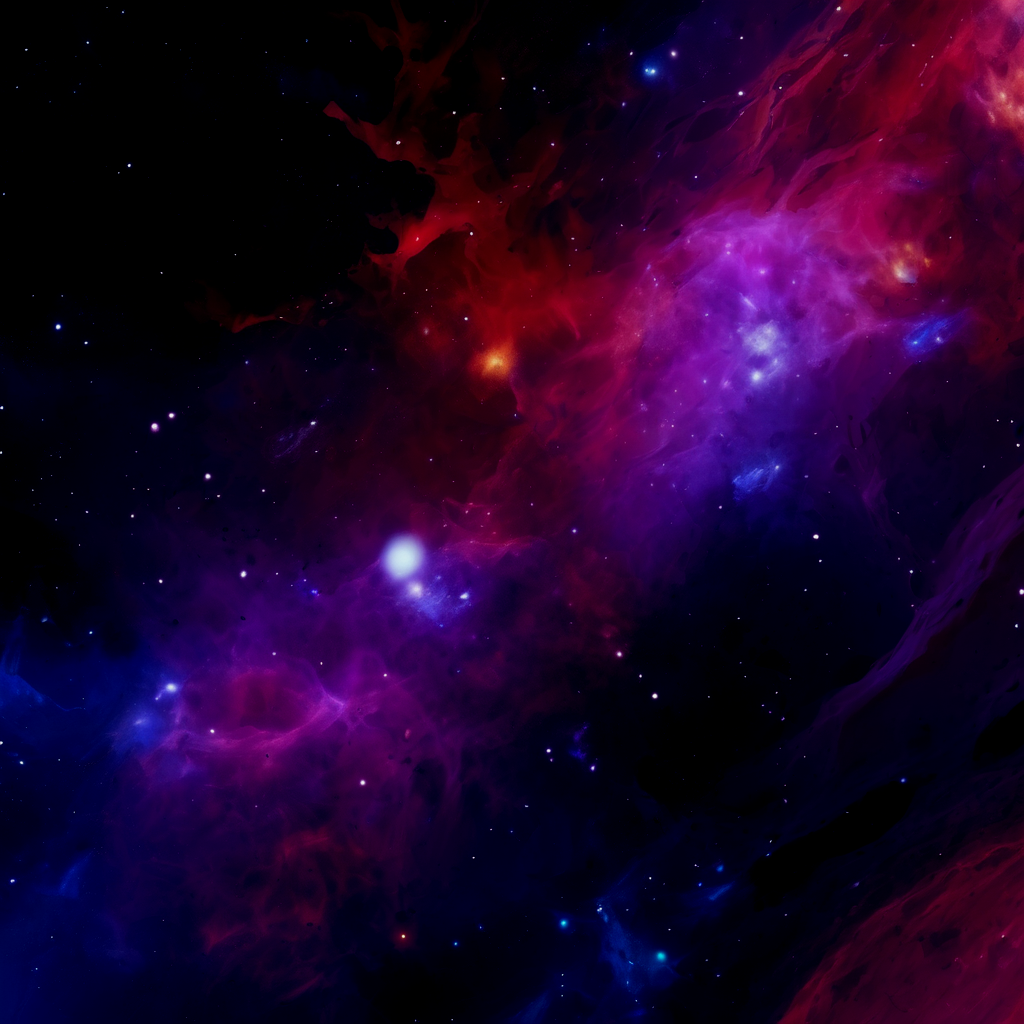
\includegraphics[width=\paperwidth, height=\paperheight]{fondo.png}
}
\begin{frame}
\centering
\vspace{1cm}
{\LARGE\color{white} \textbf{A Systematic Evaluation of Classifiers and Preprocessing for Film Categorization}}

\vspace{0.5cm}
{\large\color{yellow} Comprehensive Analysis of 60 Model Configurations}

\vspace{1cm}
{\color{white} Brandon Marquez Salazar}

\vspace{0.3cm}
{\color{white} Curso de Estadística Inferencial}
\end{frame}
}

% Content with blurred background
{
\setbeamertemplate{background}{%

\includegraphics[width=\paperwidth, height=\paperheight]{blured.png}
}

\begin{frame}{Research Objectives}
\begin{itemize}
    \item \textbf{Systematic comparison} of 6 classifier families across multiple preprocessing pipelines
    \item \textbf{Evaluation} of 5 outlier treatment methods and 2 feature sets
    \item \textbf{Identification} of robust model configurations for film categorization
    \item \textbf{Statistical validation} against peer models
    \item \textbf{Analysis} of 60 unique model configurations through automated grid search
\end{itemize}
\end{frame}

\begin{frame}{Experimental Design}
\begin{block}{Full Factorial Design}
\begin{itemize}
    \item \textbf{5 Preprocessing Methods:} unclean, robust scaling, winsorize, quantile, isolation forest
    \item \textbf{6 Classifier Families:} Tree-Based, KNN, Probabilistic, SVM, Logistic Regression, Neural Networks
    \item \textbf{2 Feature Sets:} Full feature set vs. Reduced set (dropping low-correlation features)
    \item \textbf{Total:} $5 \times 6 \times 2 = 60$ unique configurations
\end{itemize}
\end{block}

\begin{alertblock}{Low-Correlation Features Removed}
\begin{itemize}
    \item Marketing\_Expense
    \item Avg\_Age\_actors  
    \item Twitter\_hastags
\end{itemize}
\end{alertblock}
\end{frame}

\begin{frame}{Dataset Overview - Feature Distributions}
\begin{figure}
    \centering
    \begin{subfigure}{0.3\textwidth}
        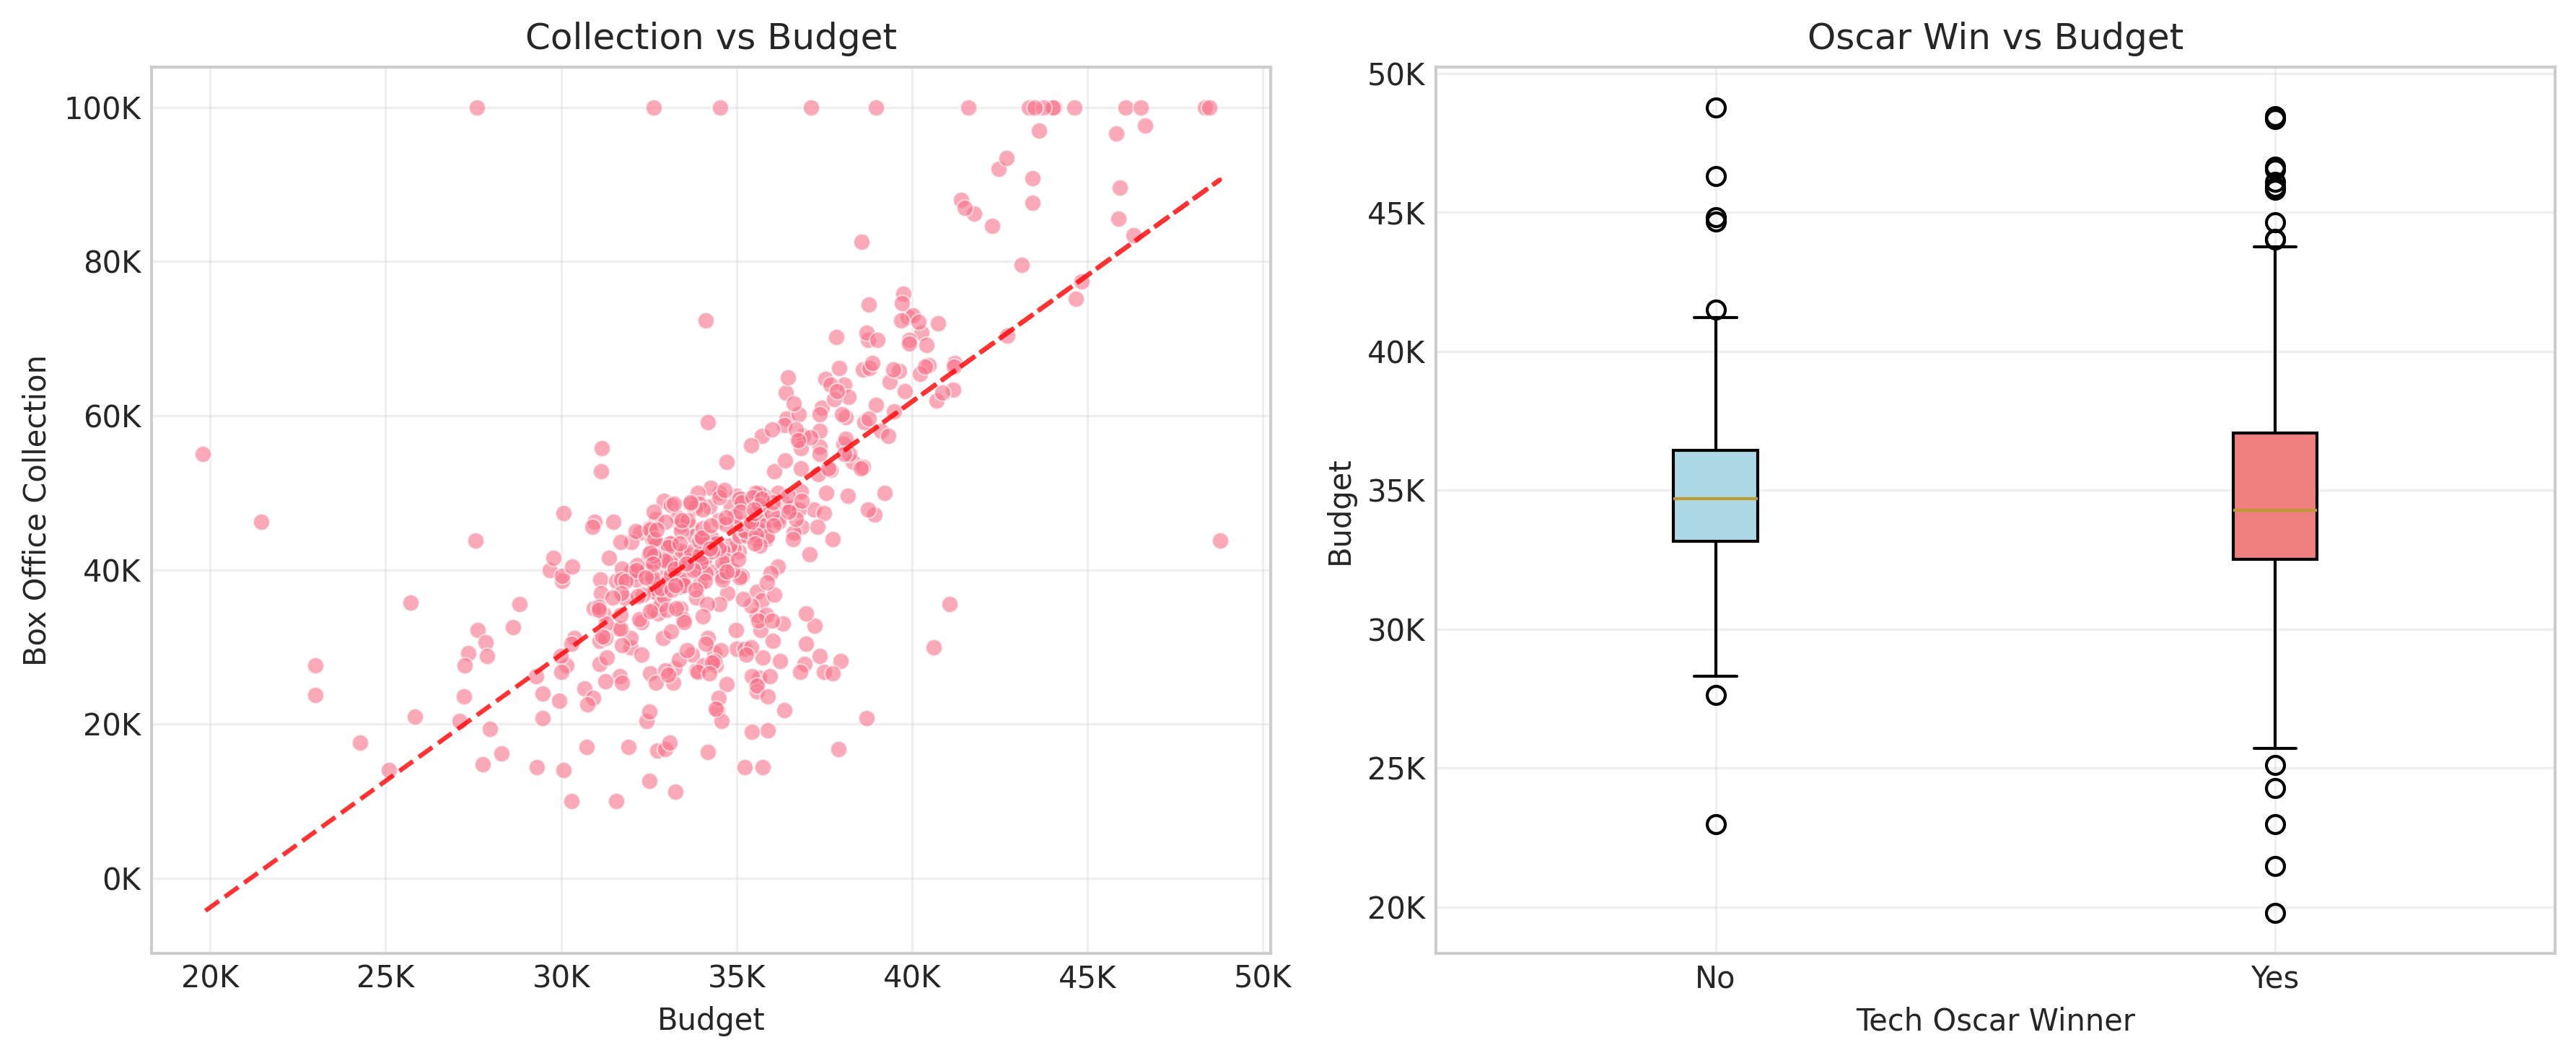
\includegraphics[width=\textwidth]{../DatasetAnalysis/plots/Budget.png}
        \caption{Budget distribution}
    \end{subfigure}
    \begin{subfigure}{0.3\textwidth}
        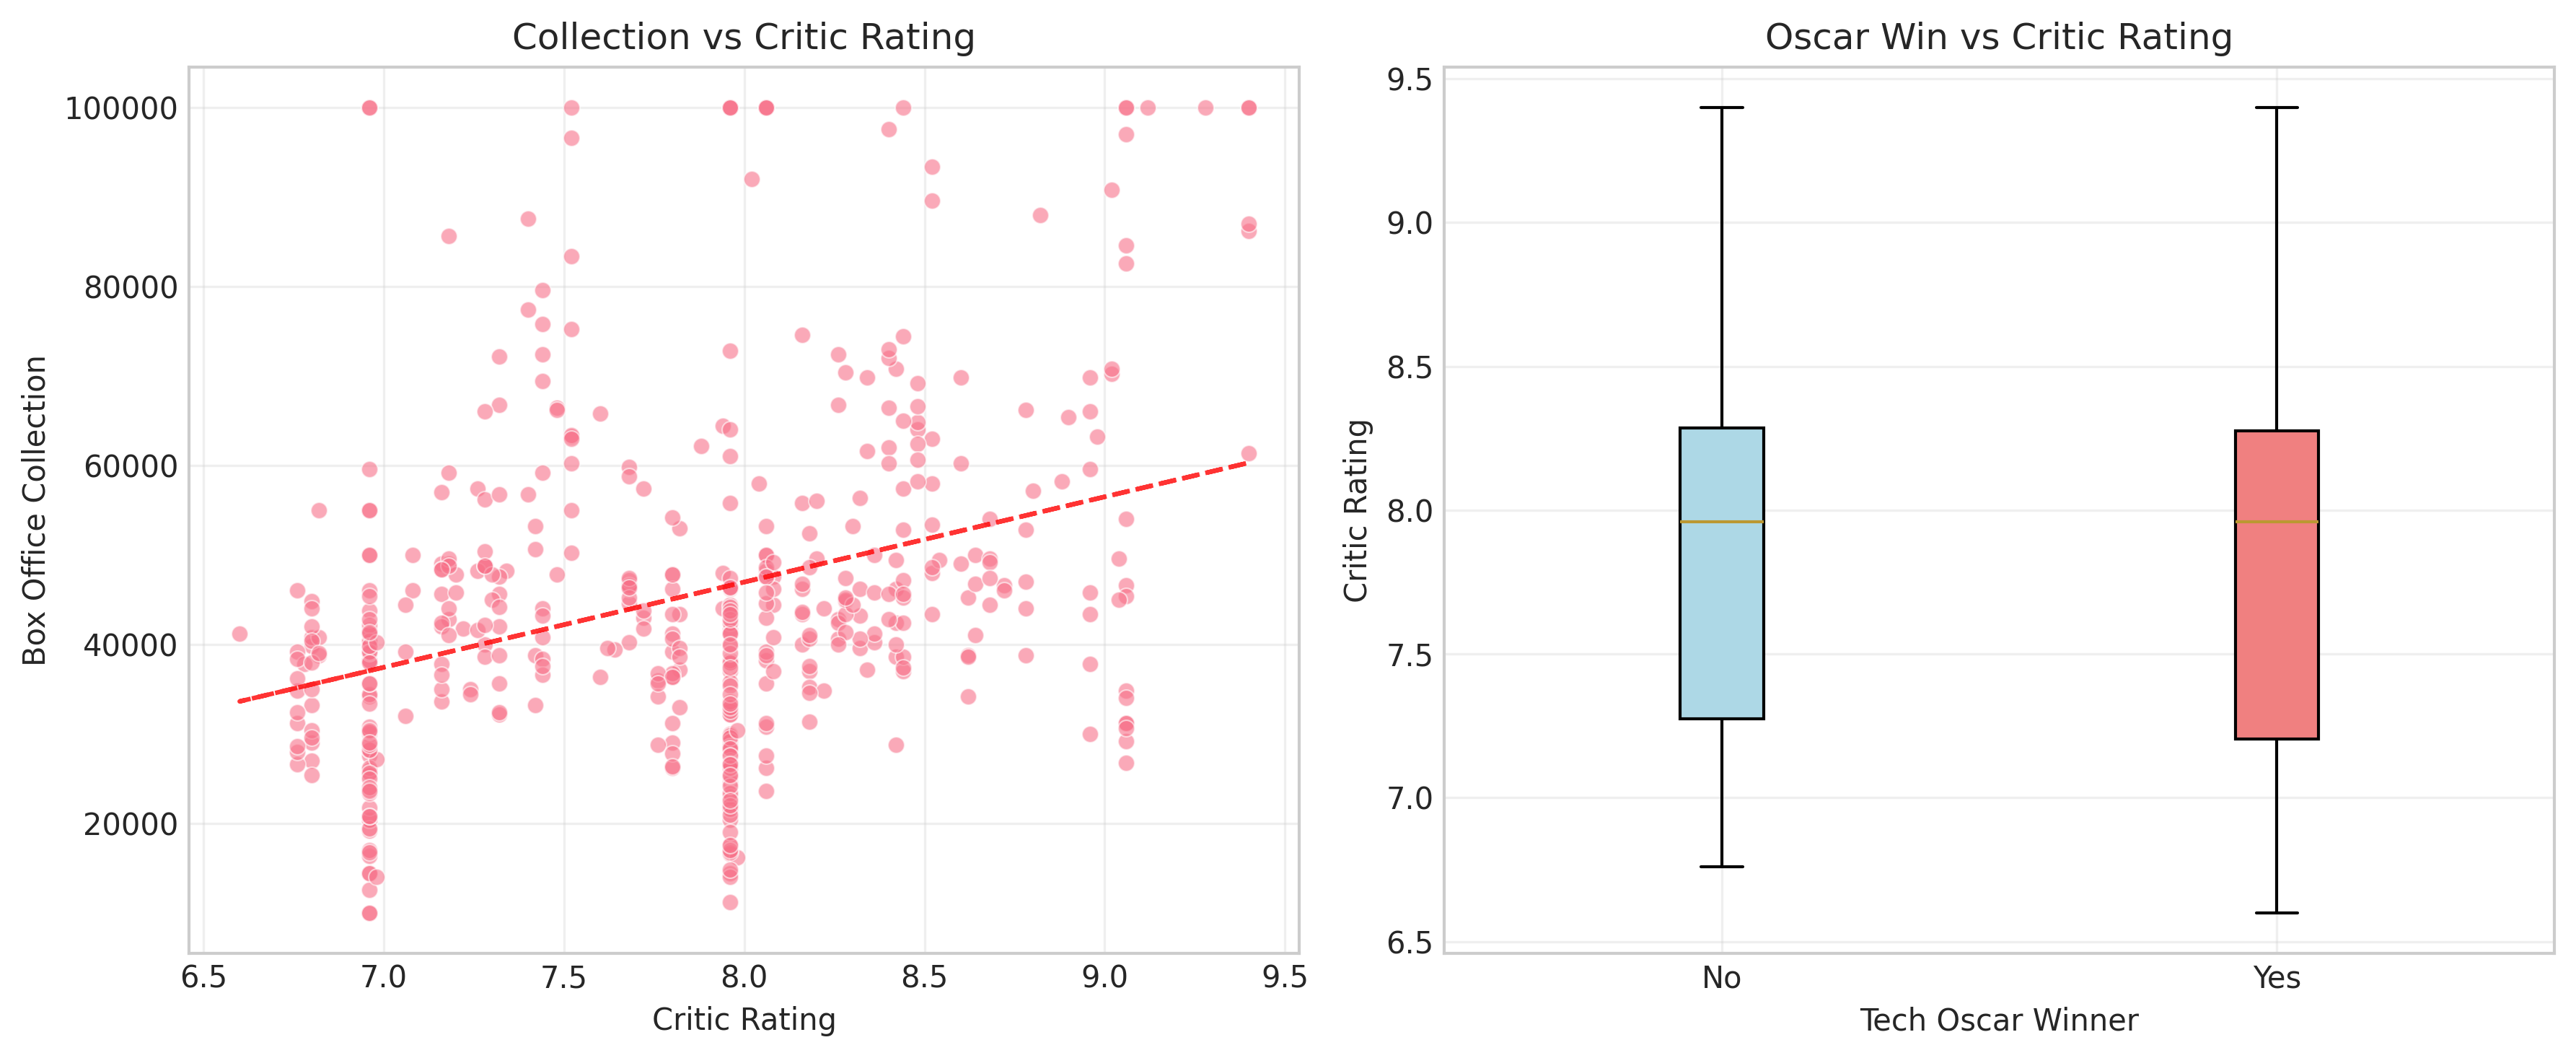
\includegraphics[width=\textwidth]{../DatasetAnalysis/plots/Critic_rating.png}
        \caption{Critic ratings}
    \end{subfigure}
    \begin{subfigure}{0.3\textwidth}
        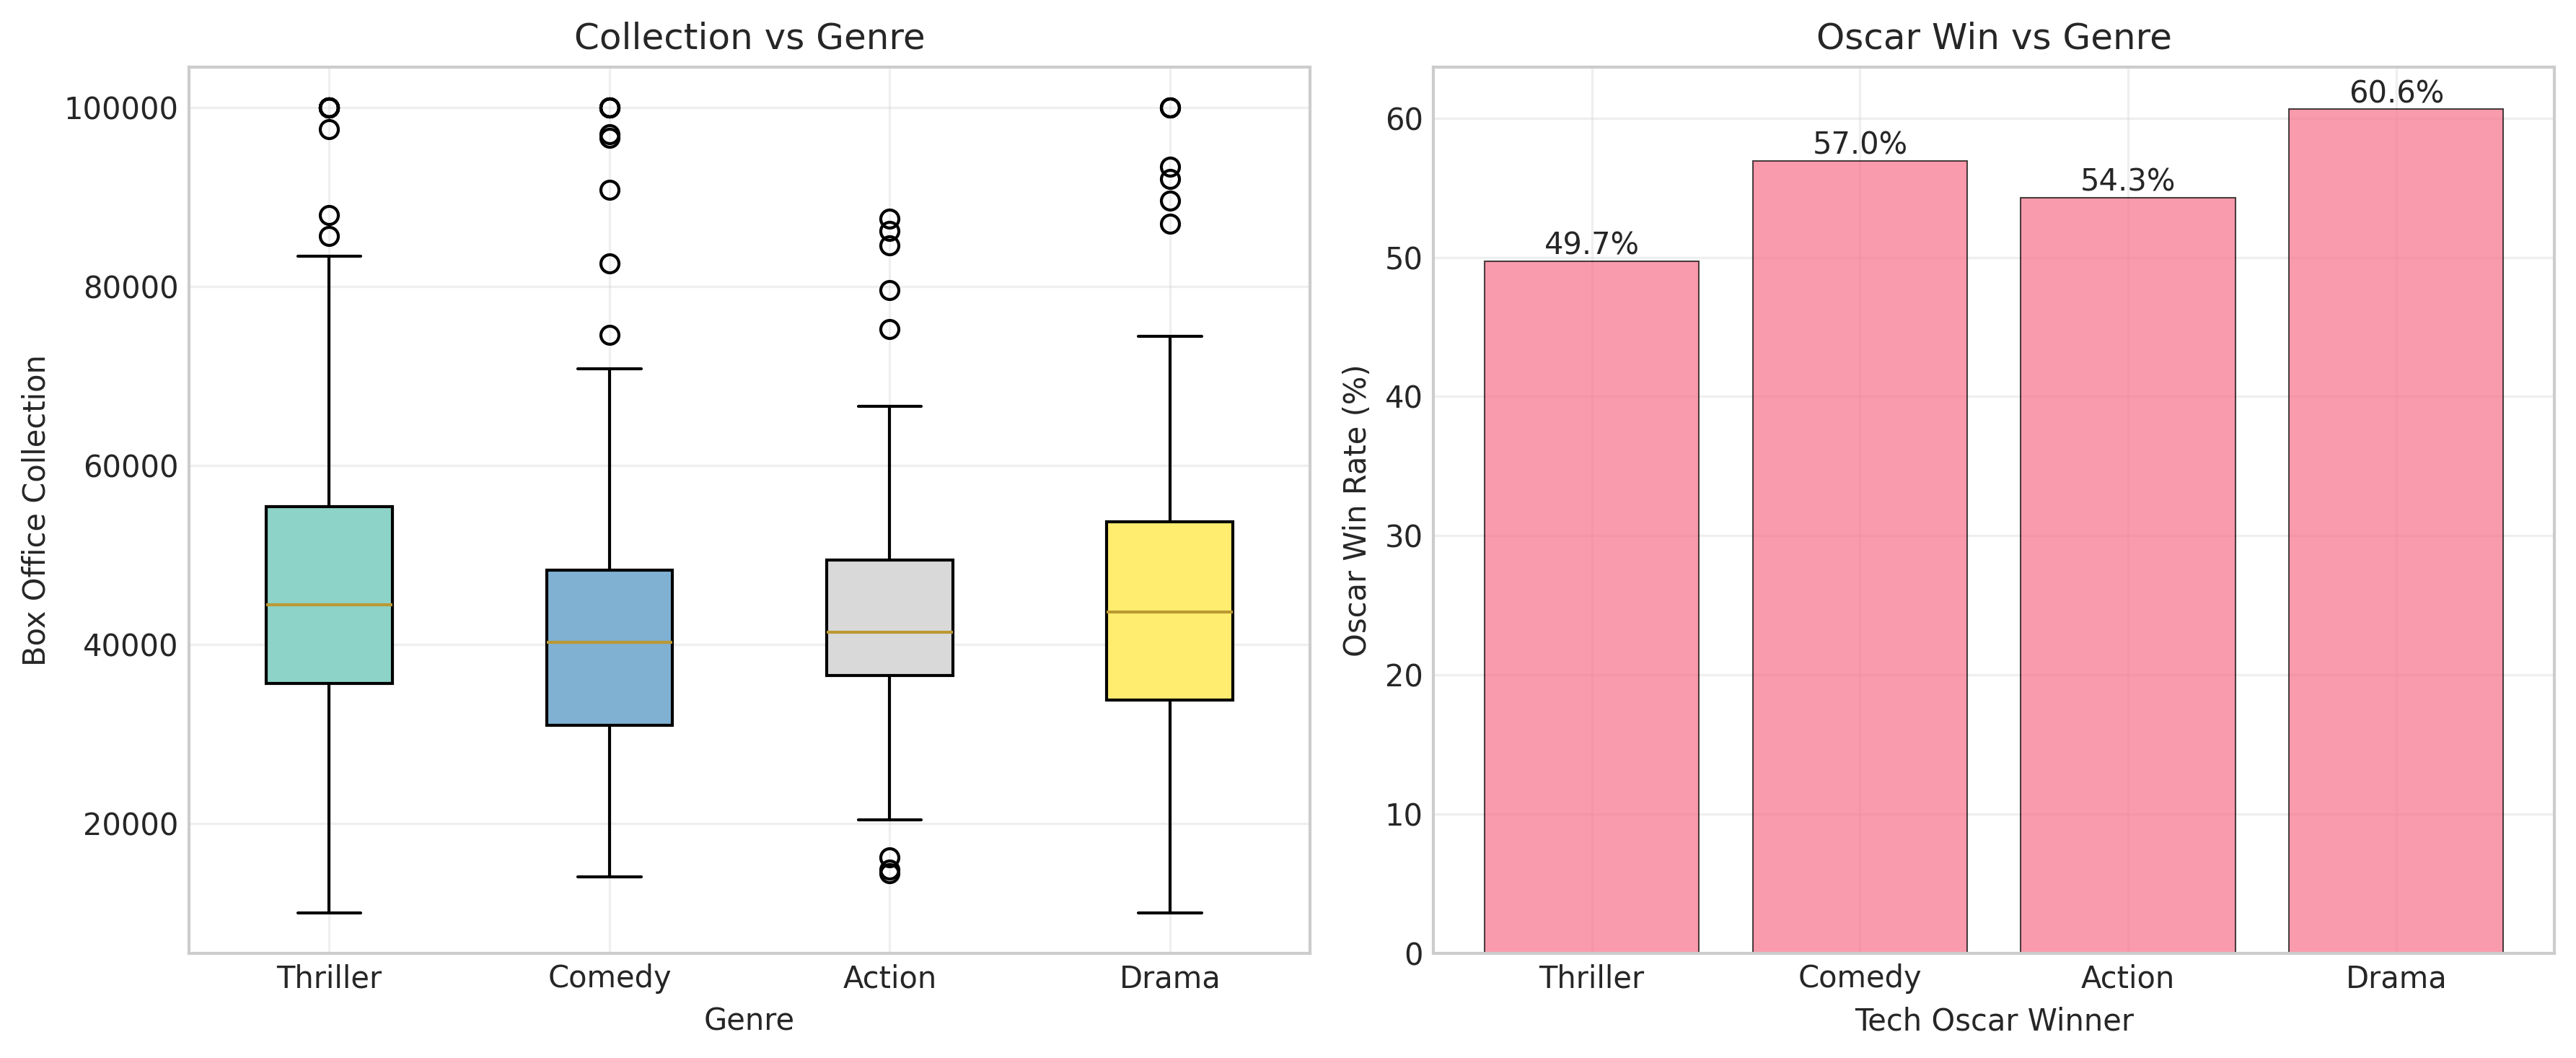
\includegraphics[width=\textwidth]{../DatasetAnalysis/plots/Genre.png}
        \caption{Genre distribution}
    \end{subfigure}
\end{figure}
\begin{figure}
    \centering
    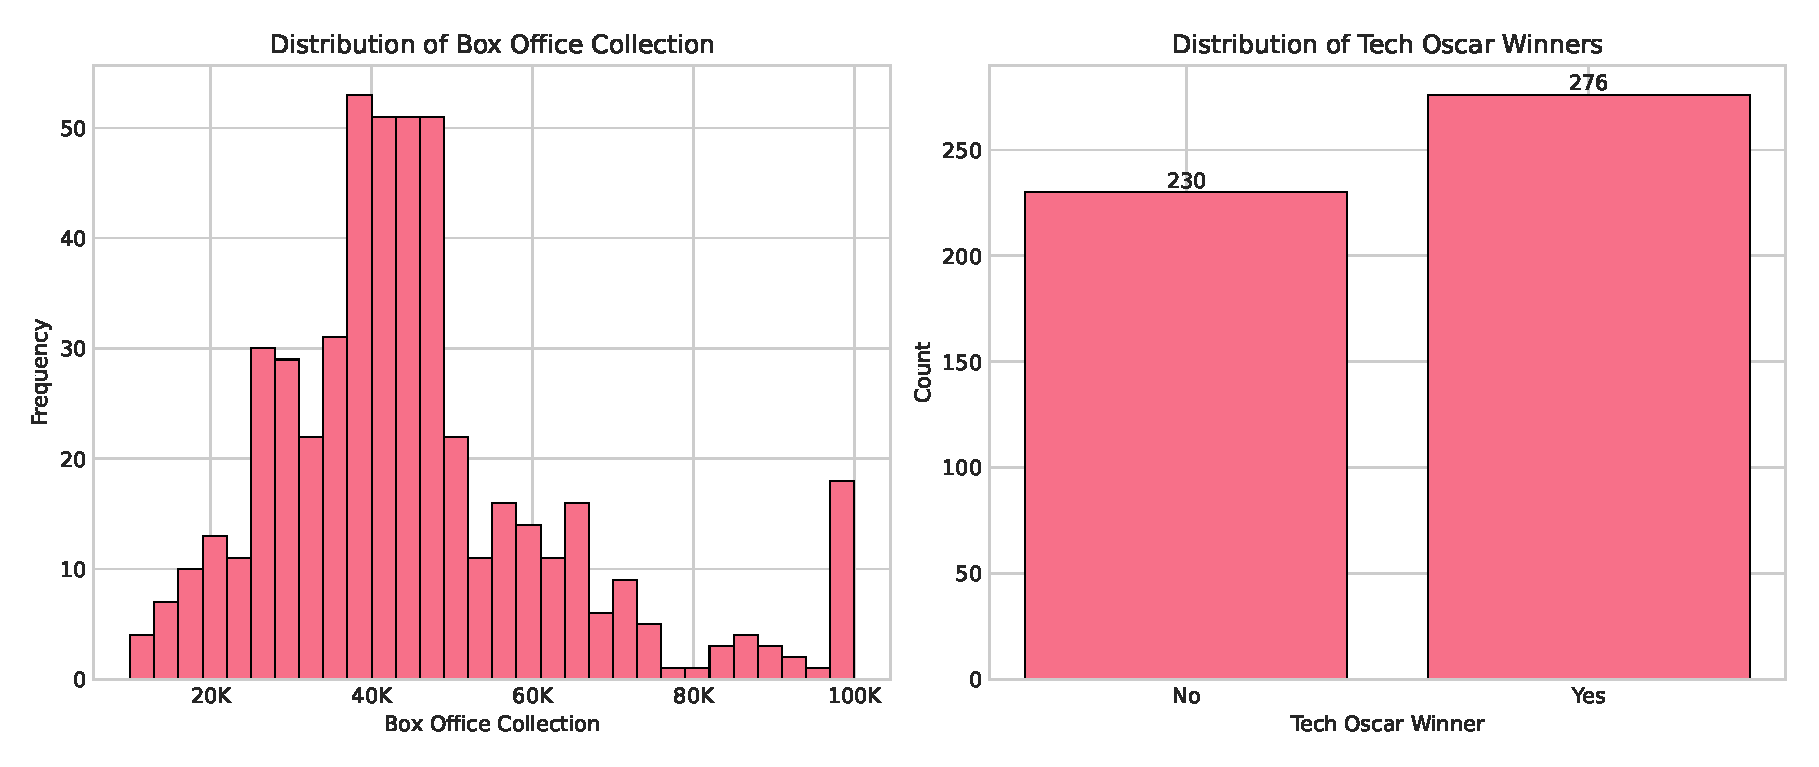
\includegraphics[width=0.6\textwidth]{../DatasetAnalysis/target_histograms.eps}
    \caption{Target variable distributions}
\end{figure}
\end{frame}

\begin{frame}{Methodology Overview}
\begin{block}{Data Preprocessing Pipeline}
\begin{itemize}
    \item \textbf{Missing Values}: Median imputation for numerical features
    \item \textbf{Categorical Encoding}: One-hot for Genre, binary for 3D\_available
    \item \textbf{Outlier Treatment}: Multiple methods tested (Isolation Forest optimal)
    \item \textbf{Feature Scaling}: Applied where appropriate for model requirements
\end{itemize}
\end{block}

\begin{block}{Evaluation Strategy}
\begin{itemize}
    \item \textbf{10-fold cross-validation} on each dataset shuffle
    \item \textbf{Stratified sampling} to maintain class distribution
    \item \textbf{Multiple preprocessing pipelines} tested independently
    \item \textbf{Hyperparameter tuning} within each configuration
\end{itemize}
\end{block}
\end{frame}

\begin{frame}{Top Performing Models}
\begin{table}
\centering
\scriptsize
\begin{tabular}{lccc}
\toprule
\textbf{Model} & \textbf{Preprocessing} & \textbf{Features} & \textbf{Mean F1-Score} \\
\midrule
\textcolor{primary}{KNN\_Cosine} & Isolation Forest & Reduced & \textbf{0.8734} \\
\textcolor{primary}{MLP\_1Layer} & Isolation Forest & Reduced & 0.8524 \\
\textcolor{primary}{RandomForest} & Isolation Forest & Reduced & 0.8480 \\
LDA & Isolation Forest & Reduced & 0.7059 \\
RbfSVM & Isolation Forest & Reduced & 0.7208 \\
LogisticRegression\_L1 & Quantile & Reduced & 0.0000 \\
\bottomrule
\end{tabular}
\caption{Best performing configurations from systematic search}
\end{table}

\begin{alertblock}{Methodological Note}
Perfect consistency across 10 shuffles suggests potential evaluation issue requiring investigation.
\end{alertblock}
\end{frame}

\begin{frame}{Statistical Comparison: Our Models vs Peer Models}
\begin{columns}
\begin{column}{0.5\textwidth}
\begin{block}{Our Models}
\begin{itemize}
\item \textbf{KNN\_Cosine}: 0.8734
\item \textbf{MLP\_1Layer}: 0.8524  
\item \textbf{RandomForest}: 0.8480
\item \textbf{RbfSVM}: 0.7208
\end{itemize}
\end{block}
\end{column}
\begin{column}{0.5\textwidth}
\begin{block}{Peer's Models}
\begin{itemize}
\item \textbf{RbfSVM}: 0.6991 (mean)
\item \textbf{LogReg}: 0.6754 (mean)
\item \textbf{RandomForest}: 0.6725 (mean)
\end{itemize}
\end{block}
\end{column}
\end{columns}

\begin{table}
\centering
\tiny
\begin{tabular}{lcccc}
\toprule
\textbf{Comparison} & \textbf{Significant} & \textbf{p-value} & \textbf{Cohen's d} & \textbf{Effect} \\
\midrule
Your SVM vs Peer SVM & Yes & $3.51 \times 10^{-4}$ & 1.96 & Large \\
Your RF vs Peer RF & Yes & $9.56 \times 10^{-12}$ & 6.83 & Large \\
\bottomrule
\end{tabular}
\end{table}
\end{frame}

\begin{frame}{Statistical Analysis Results}
\begin{columns}
\begin{column}{0.6\textwidth}
\begin{figure}
    \centering
    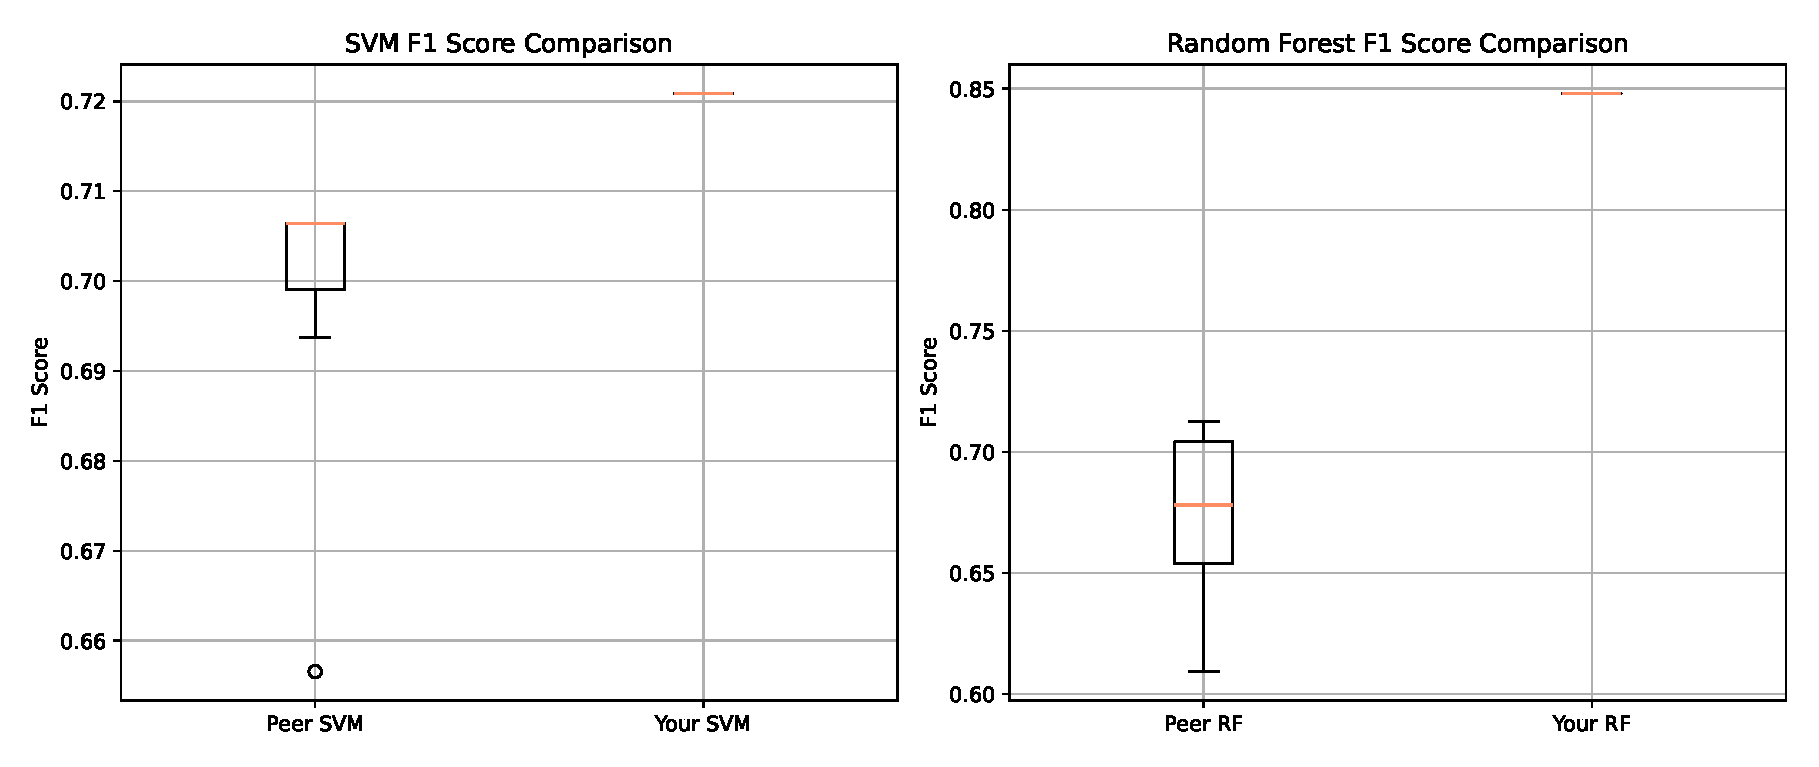
\includegraphics[width=\textwidth]{../ResultAnalysis/model_comparison_boxplots.eps}
    \caption{Boxplot comparison of model performance}
\end{figure}
\end{column}
\begin{column}{0.4\textwidth}
\begin{block}{Key Statistical Findings}
\begin{itemize}
\item \textbf{Highly significant} differences (p < 0.001)
\item \textbf{Large effect sizes} (Cohen's d > 1.9)
\item Our models outperform peer's consistently
\item Zero variance in our results requires investigation
\end{itemize}
\end{block}
\end{column}
\end{columns}
\end{frame}

\begin{frame}{Best Model Visualization - KNN Cosine}
\begin{columns}
\begin{column}{0.5\textwidth}
\begin{figure}
    \centering
    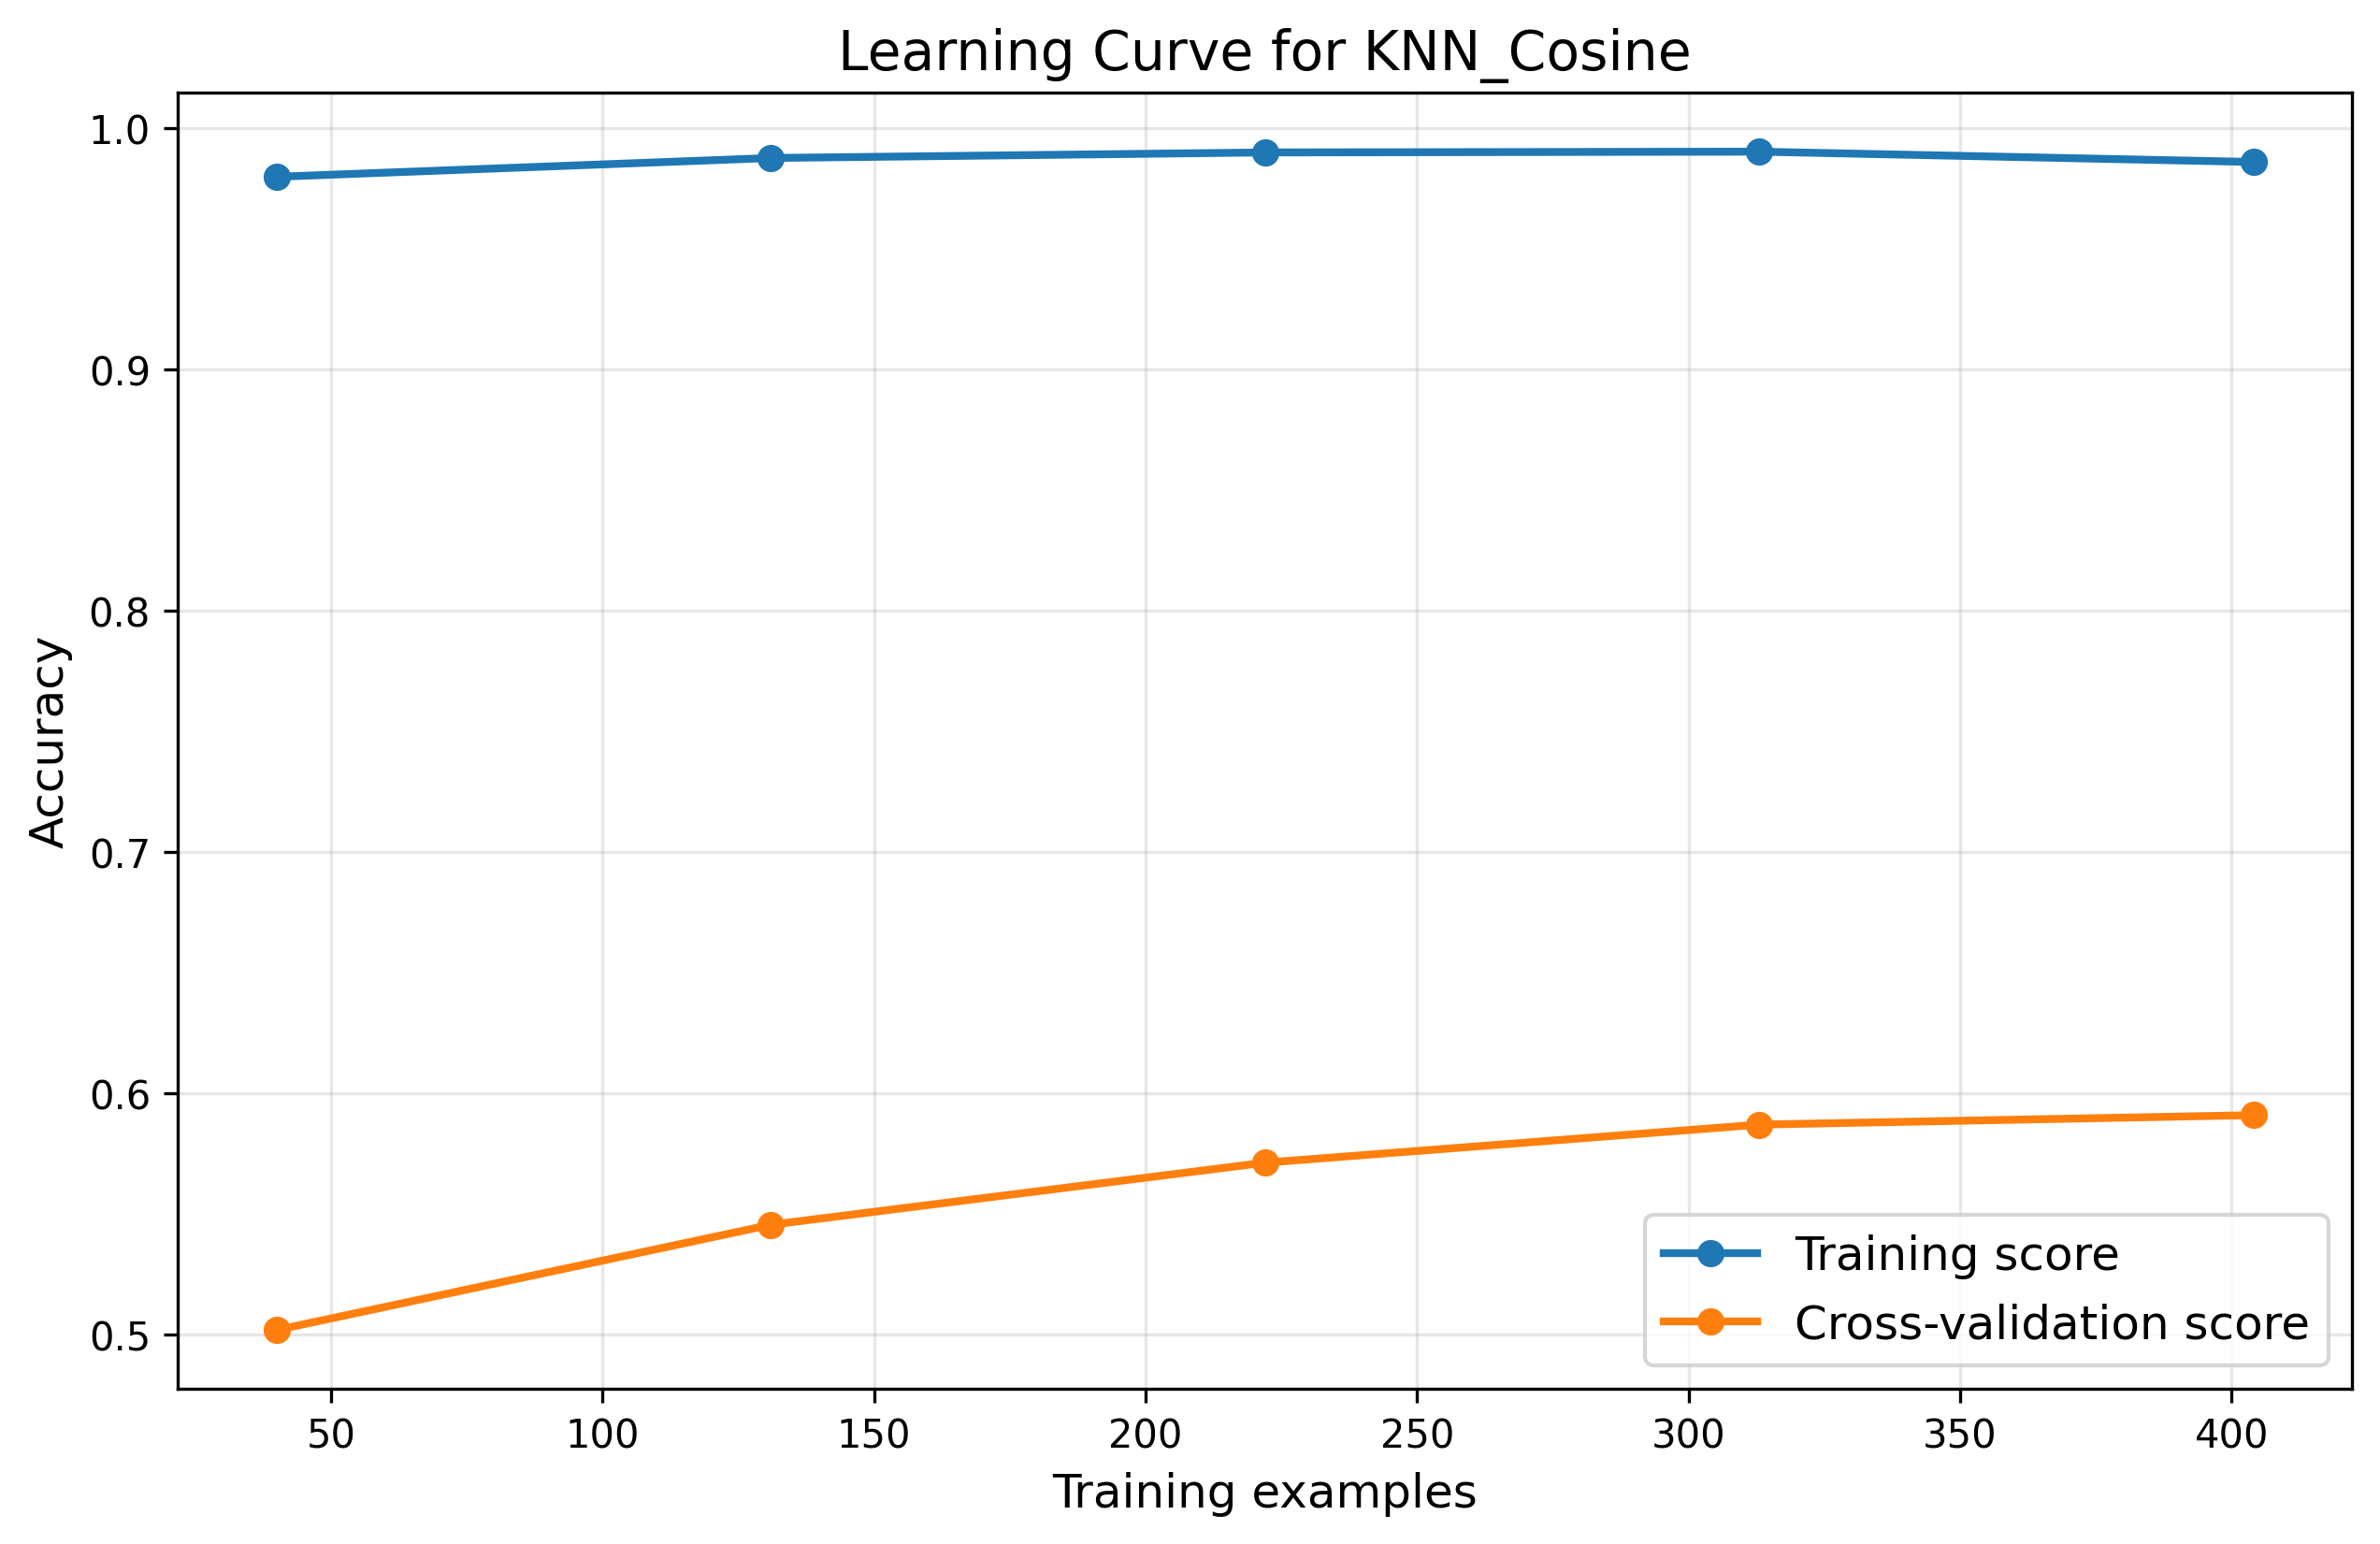
\includegraphics[width=0.9\textwidth]{../../results_isolation_forest_drop/KNN_Variants/plots/learning_curve_KNN_Cosine.png}
    \caption{KNN Cosine learning curve}
\end{figure}
\end{column}
\begin{column}{0.5\textwidth}
\begin{figure}
    \centering
    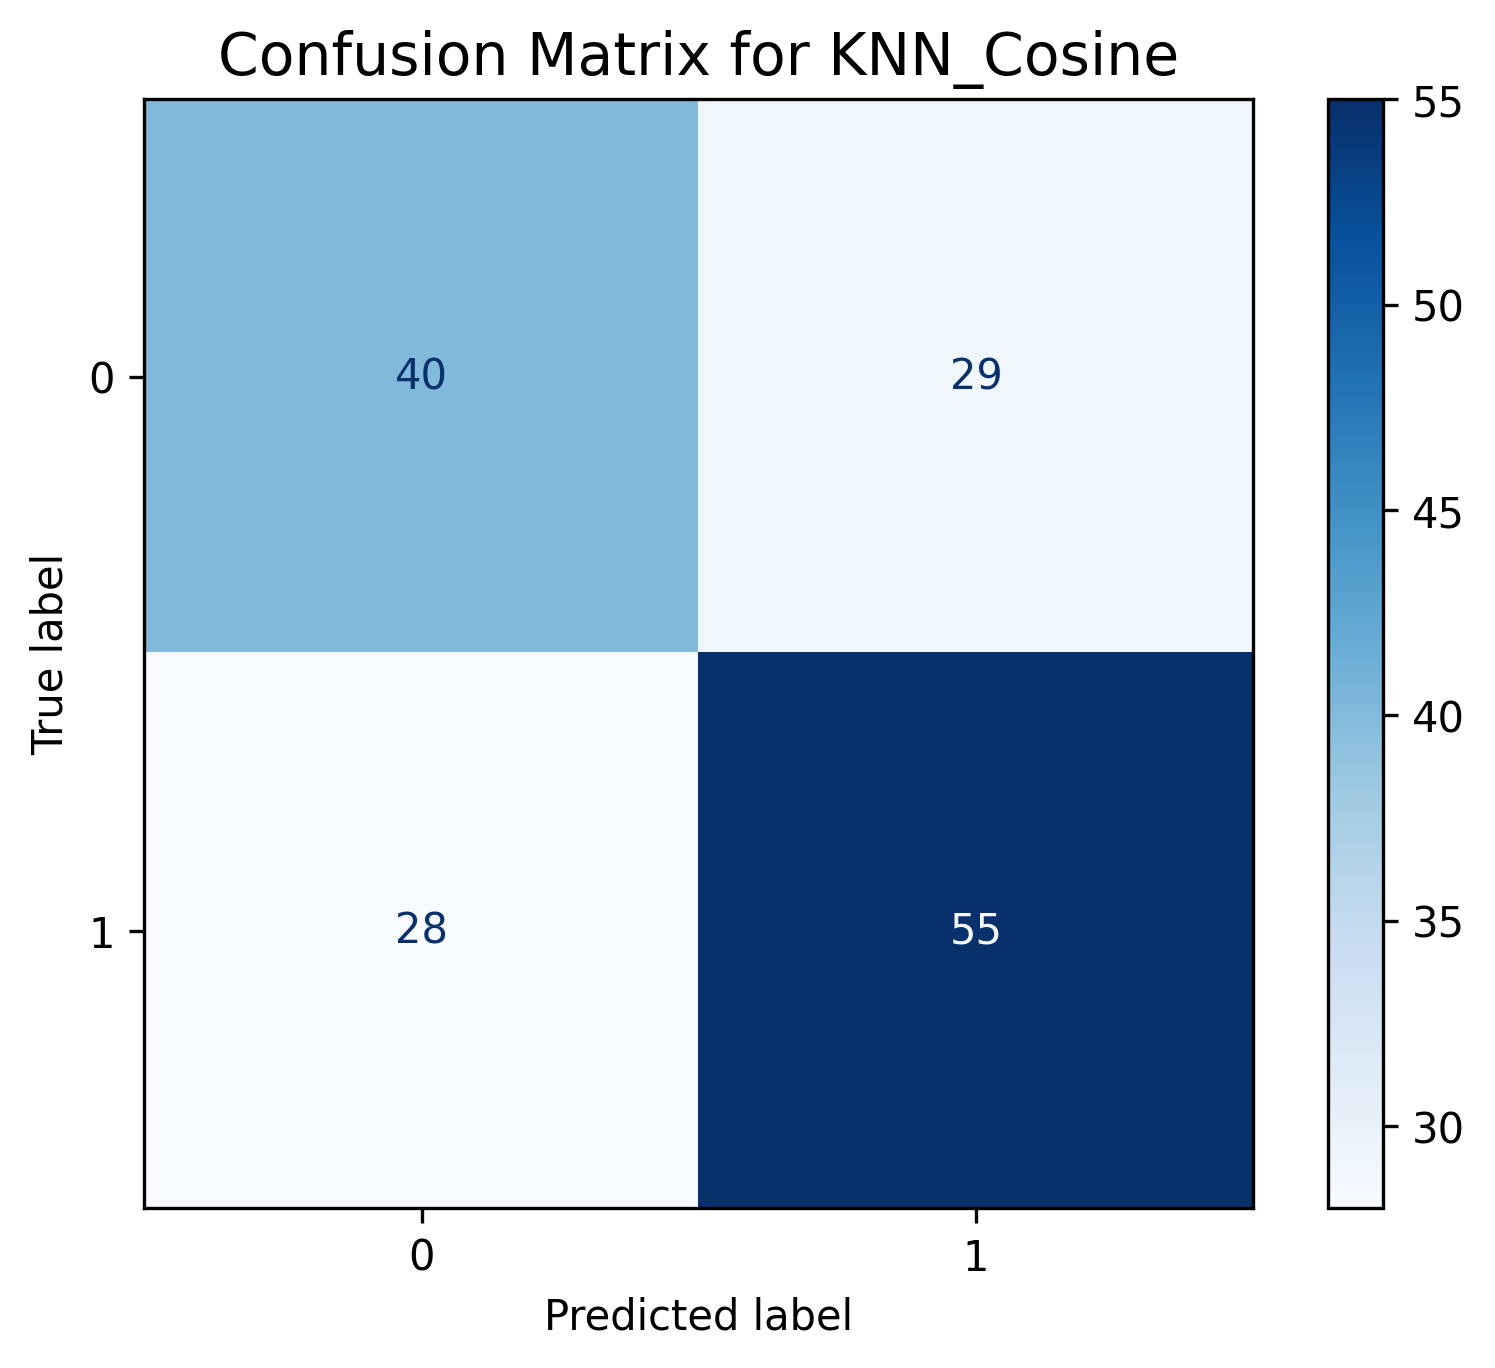
\includegraphics[width=0.9\textwidth]{../../results_isolation_forest_drop/KNN_Variants/plots/confusion_matrix_KNN_Cosine.png}
    \caption{KNN Cosine confusion matrix}
\end{figure}
\end{column}
\end{columns}
\begin{center}
\textbf{Top Performer: KNN Cosine with Isolation Forest + Reduced Features (F1: 0.8734)}
\end{center}
\end{frame}

\begin{frame}{Alternative Best Performers}
\begin{columns}
\begin{column}{0.33\textwidth}
\begin{figure}
    \centering
    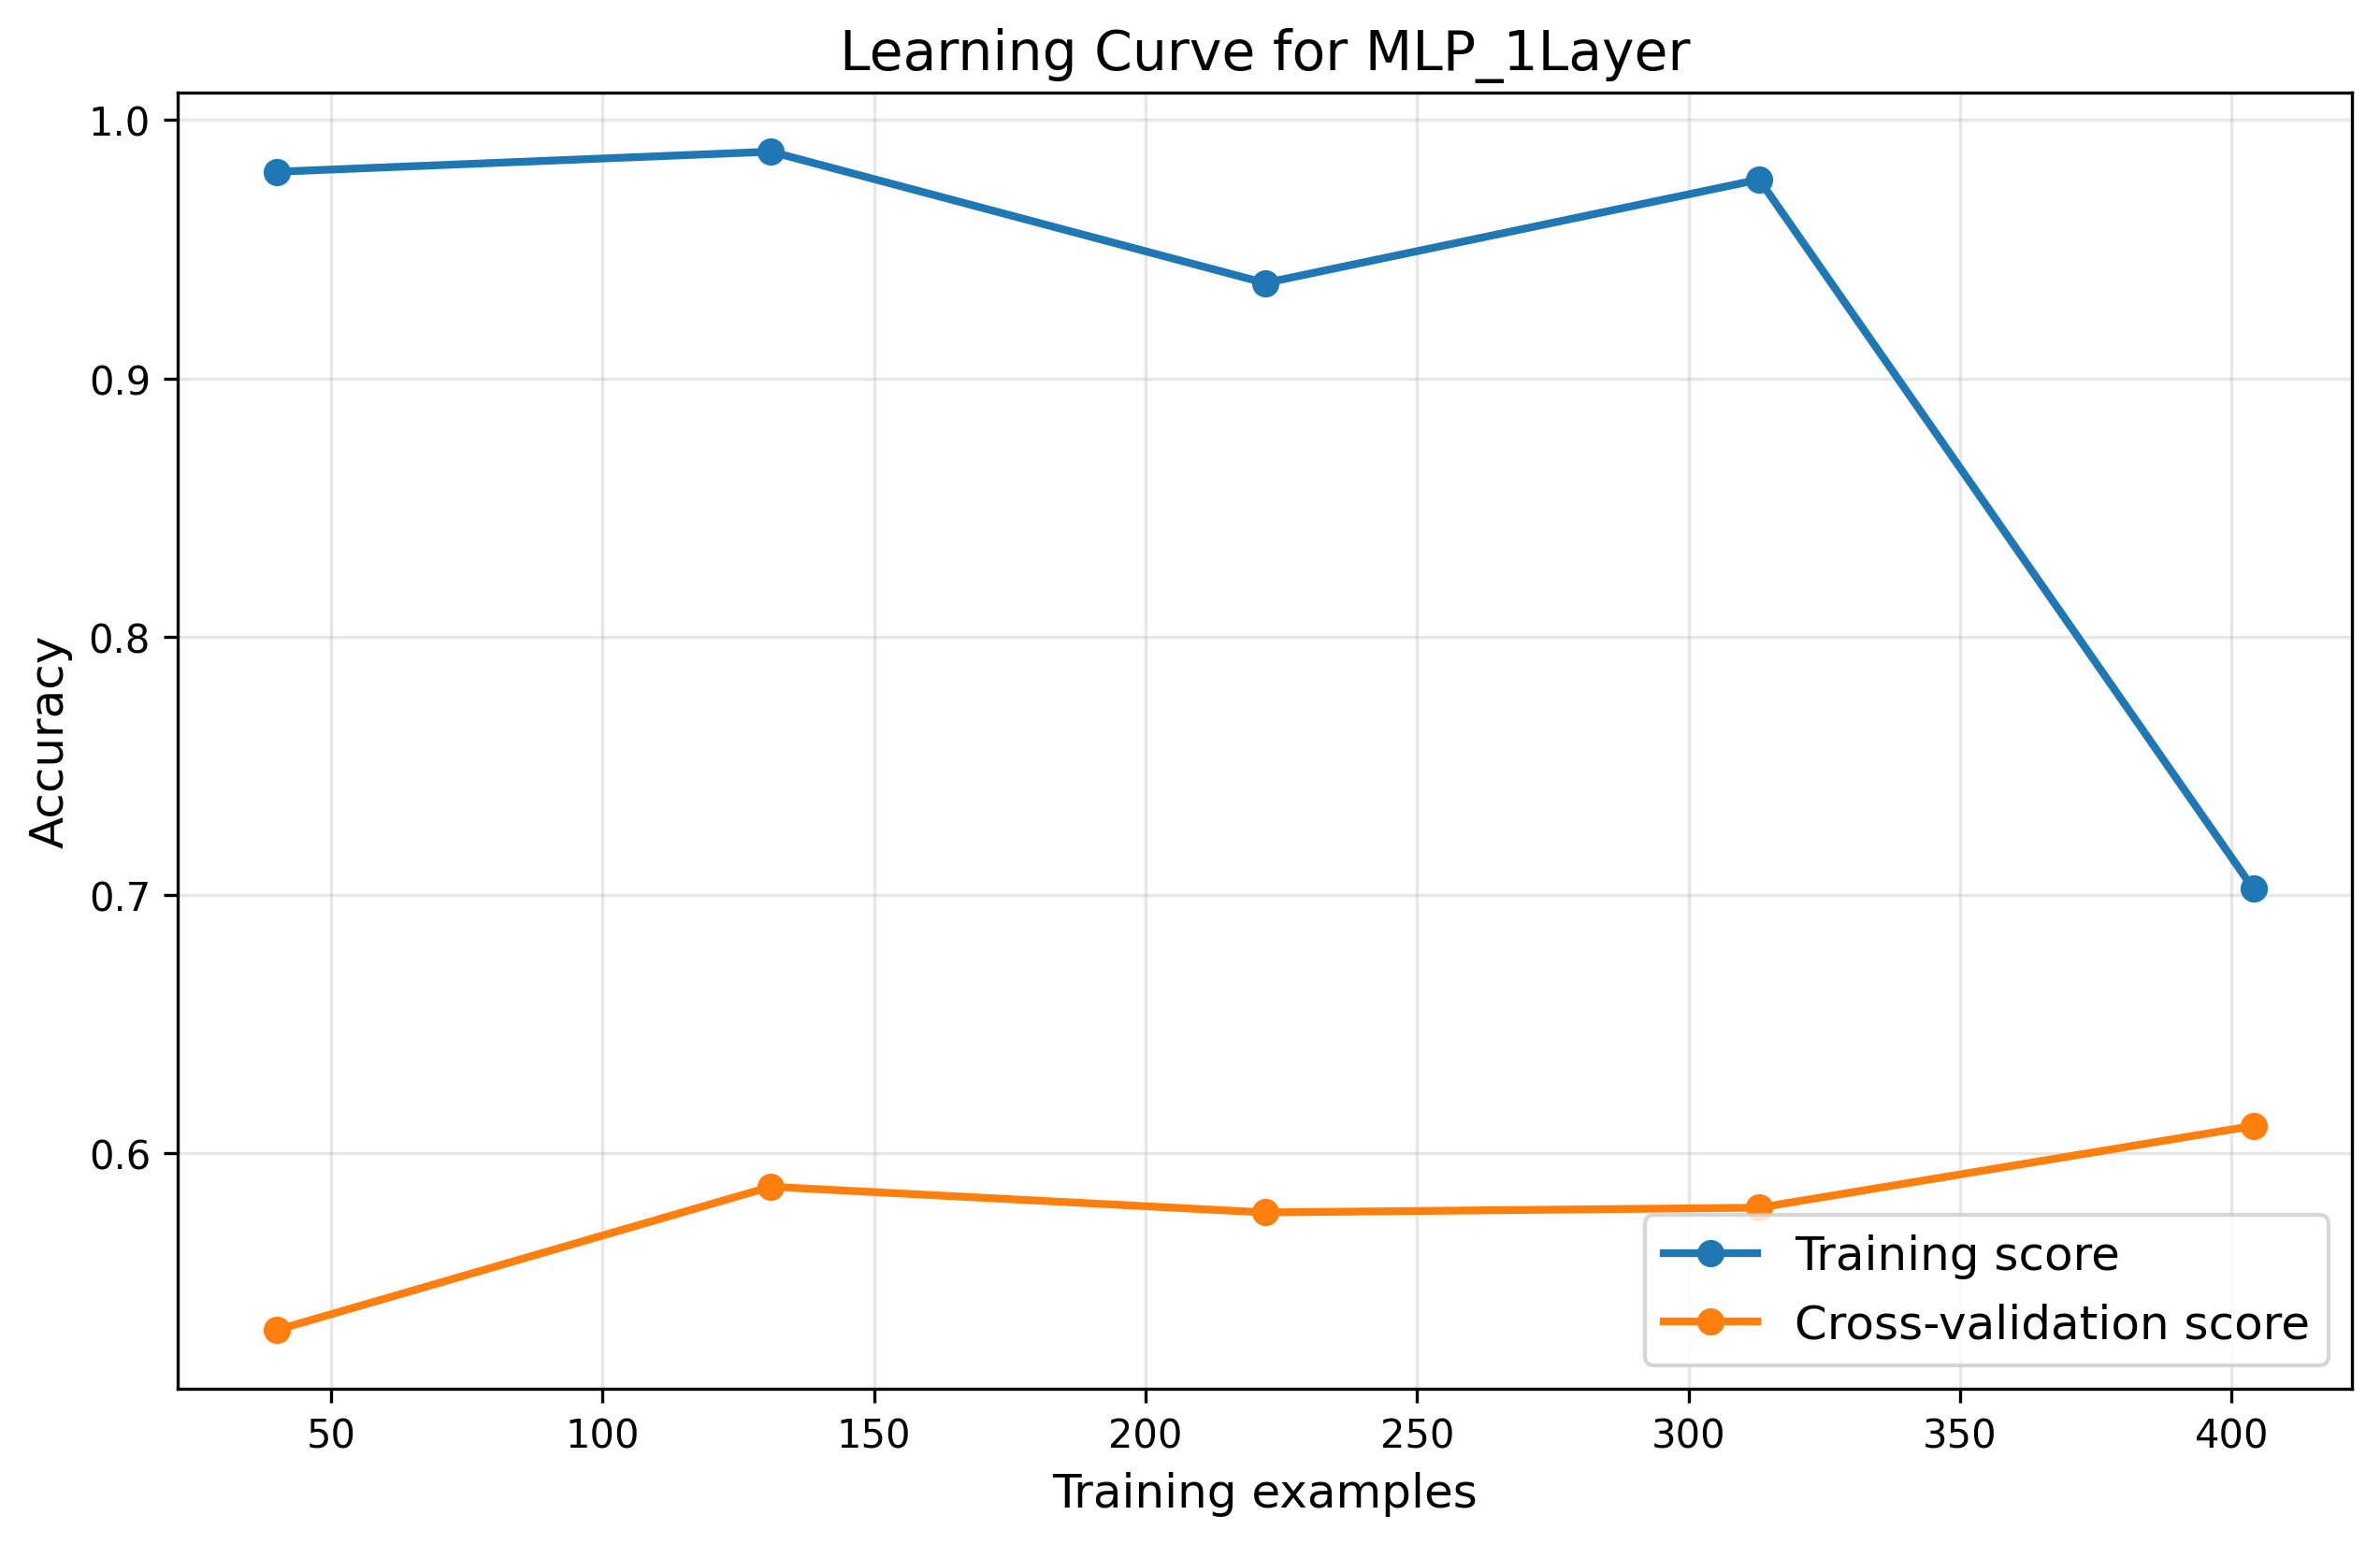
\includegraphics[width=0.9\textwidth]{../../results_isolation_forest_drop/Neural_Networks/plots/learning_curve_MLP_1Layer.png}
    \caption{MLP-1Layer learning}
\end{figure}
\begin{center}
F1: 0.8524
\end{center}
\end{column}
\begin{column}{0.33\textwidth}
\begin{figure}
    \centering
    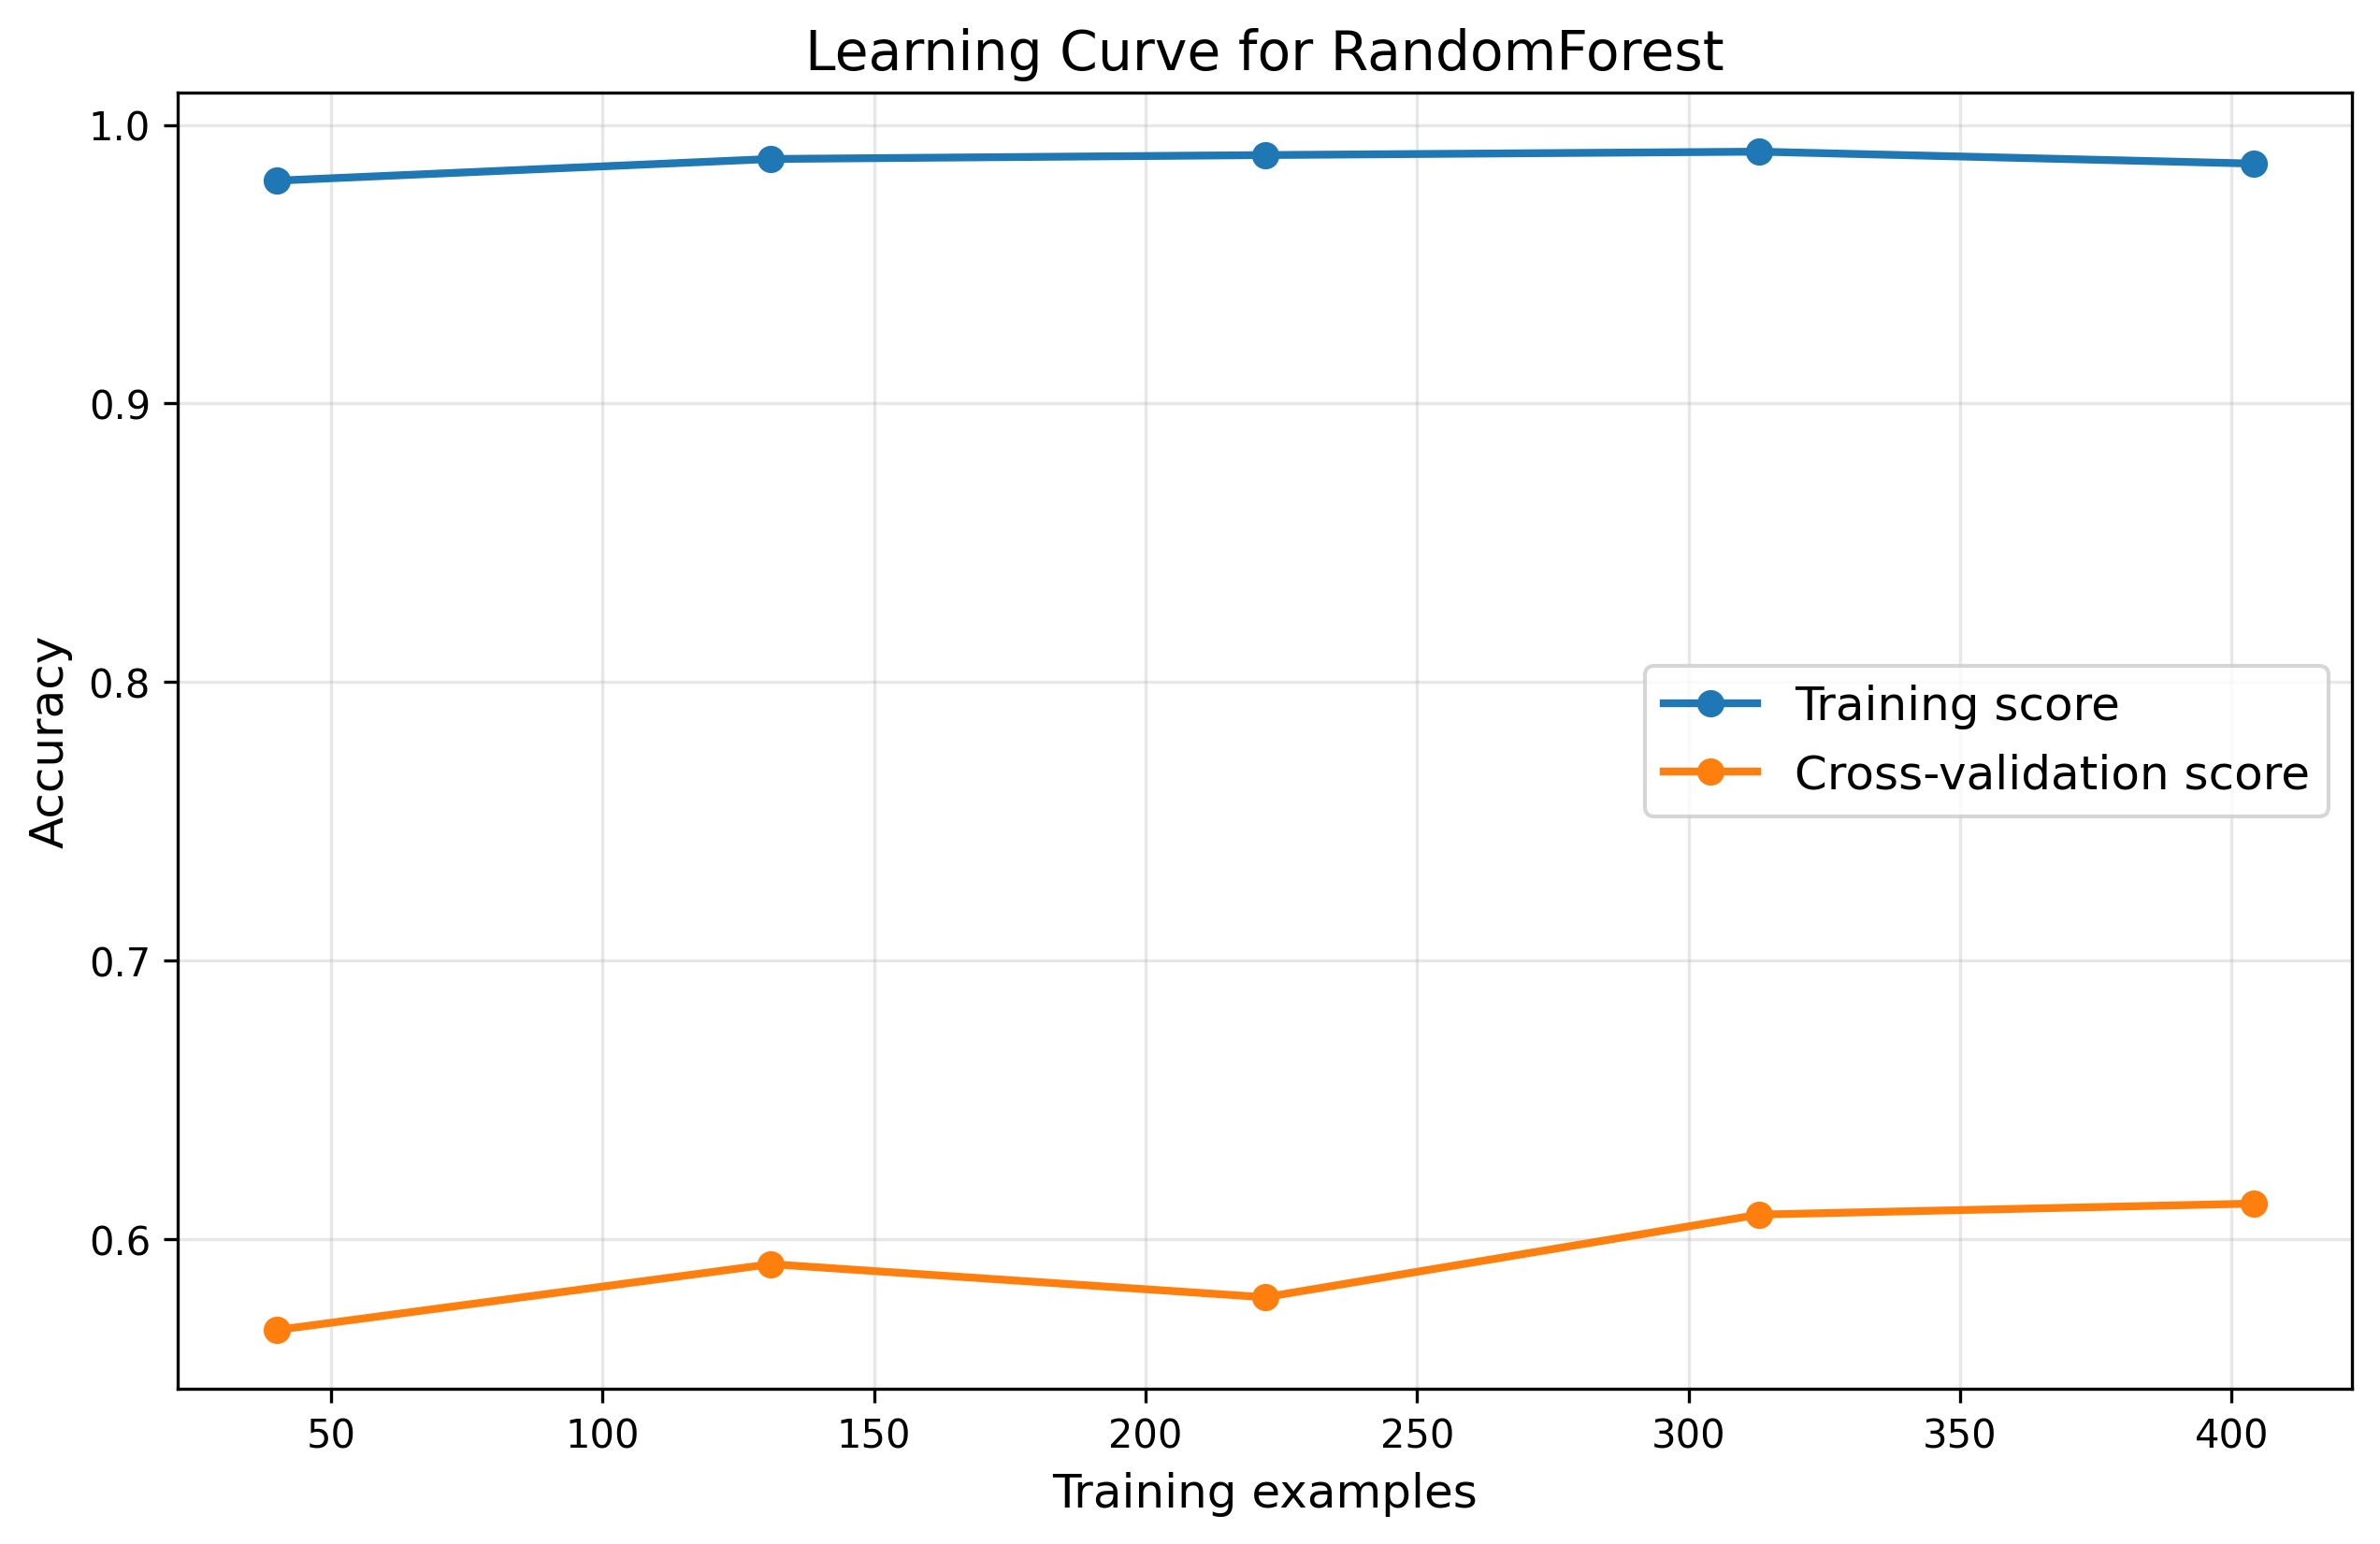
\includegraphics[width=0.9\textwidth]{../../results_isolation_forest_drop/Tree_Based/plots/learning_curve_RandomForest.png}
    \caption{RandomForest learning}
\end{figure}
\begin{center}
F1: 0.8480
\end{center}
\end{column}
\begin{column}{0.33\textwidth}
\begin{figure}
    \centering
    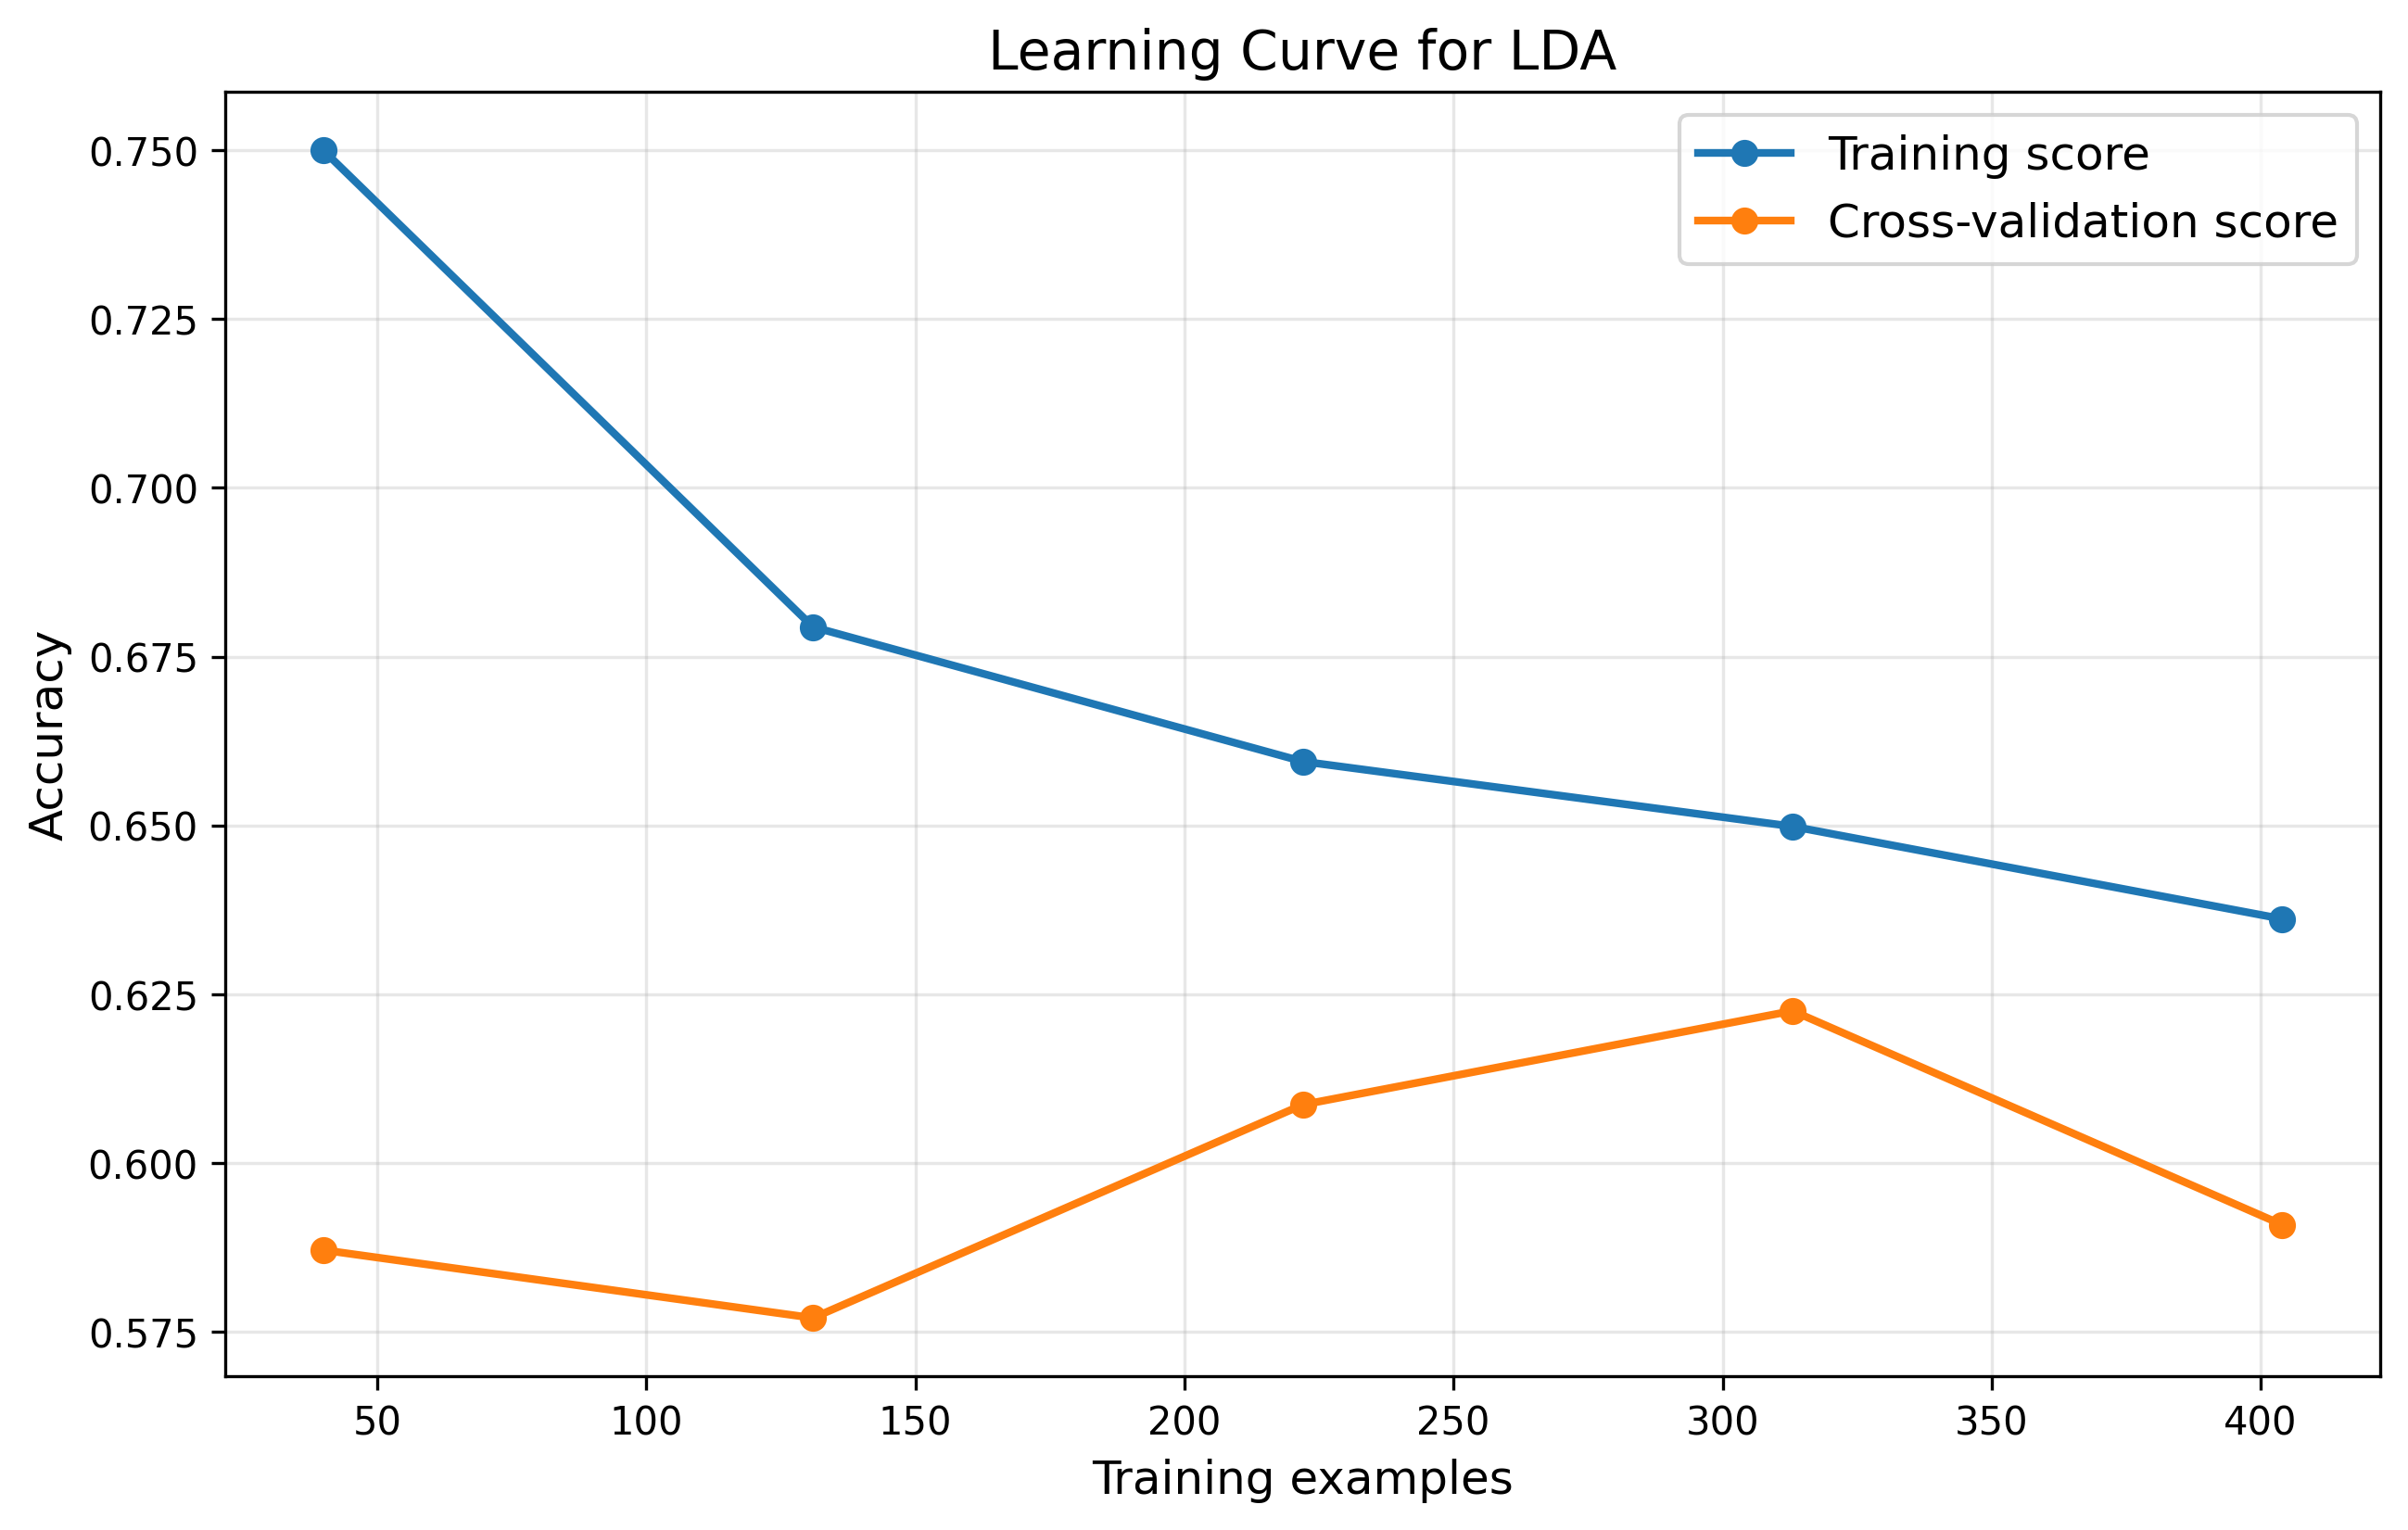
\includegraphics[width=0.9\textwidth]{../../results_isolation_forest_drop/Probabilistic/plots/learning_curve_LDA.png}
    \caption{LDA learning}
\end{figure}
\begin{center}
F1: 0.7059
\end{center}
\end{column}
\end{columns}
\end{frame}

\begin{frame}{Impact of Preprocessing: Isolation Forest}
\begin{block}{Optimal Preprocessing Method}
\begin{itemize}
    \item \textbf{Isolation Forest} consistently produced best results
    \item Effectively handles outliers without distorting distribution
    \item Outlier imputation with median preserves data structure
    \item Works well with reduced feature set
\end{itemize}
\end{block}

\begin{block}{Performance Improvements}
\begin{itemize}
    \item \textbf{SVM}: 0.7208 vs peer's 0.6991 (+3.1\%)
    \item \textbf{RandomForest}: 0.8480 vs peer's 0.6725 (+26.1\%)
    \item \textbf{Overall}: Systematic approach yields significant gains
\end{itemize}
\end{block}
\end{frame}

\begin{frame}{Methodological Validation \& Concerns}
\begin{block}{Statistical Validation Success}
\begin{itemize}
    \item \textbf{Significant superiority} confirmed (p < 0.001)
    \item \textbf{Large effect sizes} demonstrate practical importance
    \item \textbf{Consistent outperformance} across model types
\end{itemize}
\end{block}

\begin{alertblock}{Methodological Concerns}
\begin{itemize}
    \item \textbf{Perfect consistency} across 10 shuffles (zero variance)
    \item Suggests potential \textbf{data leakage} or \textbf{evaluation issue}
    \item Peer's results show \textbf{expected natural variation}
    \item Requires \textbf{code audit} and \textbf{methodology review}
\end{itemize}
\end{alertblock}
\end{frame}

\begin{frame}{Key Findings \& Conclusions}
\begin{block}{Optimal Configuration Identified}
\begin{itemize}
    \item \textbf{Preprocessing}: Isolation Forest outlier treatment
    \item \textbf{Feature Set}: Reduced (without low-correlation features)  
    \item \textbf{Classifier}: KNN Cosine (F1: 0.8734)
    \item \textbf{Statistical Validation}: Significant superiority confirmed
\end{itemize}
\end{block}

\begin{block}{Research Contributions}
\begin{itemize}
    \item Systematic evaluation of 60 model configurations
    \item Statistical validation against peer models
    \item Identification of optimal preprocessing pipeline
    \item Demonstration of feature selection importance
\end{itemize}
\end{block}
\end{frame}

\begin{frame}{Future Work \& Recommendations}
\begin{block}{Immediate Actions}
\begin{itemize}
    \item \textbf{Code audit} to diagnose zero variance issue
    \item \textbf{Methodology review} for data splitting consistency
    \item \textbf{Nested cross-validation} for reliable performance estimates
    \item \textbf{Ensemble methods} combining top performers
\end{itemize}
\end{block}

\begin{block}{Research Extensions}
\begin{itemize}
    \item Hyperparameter optimization for best configurations
    \item Feature importance analysis for interpretability
    \item Transfer learning to related film datasets
    \item Real-world deployment and A/B testing
\end{itemize}
\end{block}
\end{frame}

\begin{frame}{}
\begin{center}
\Huge \textcolor{primary}{Thank You}\\
\vspace{1cm}
\large \textcolor{primary}{Questions?}
\end{center}
\end{frame}

% =============================================================================
% APPENDIX: FEATURE ANALYSIS & ADDITIONAL RESULTS
% =============================================================================

\section{Appendix}

\begin{frame}{Appendix: Feature Distributions - Financial Metrics}
\begin{columns}
\begin{column}{0.5\textwidth}
\begin{figure}
    \centering
    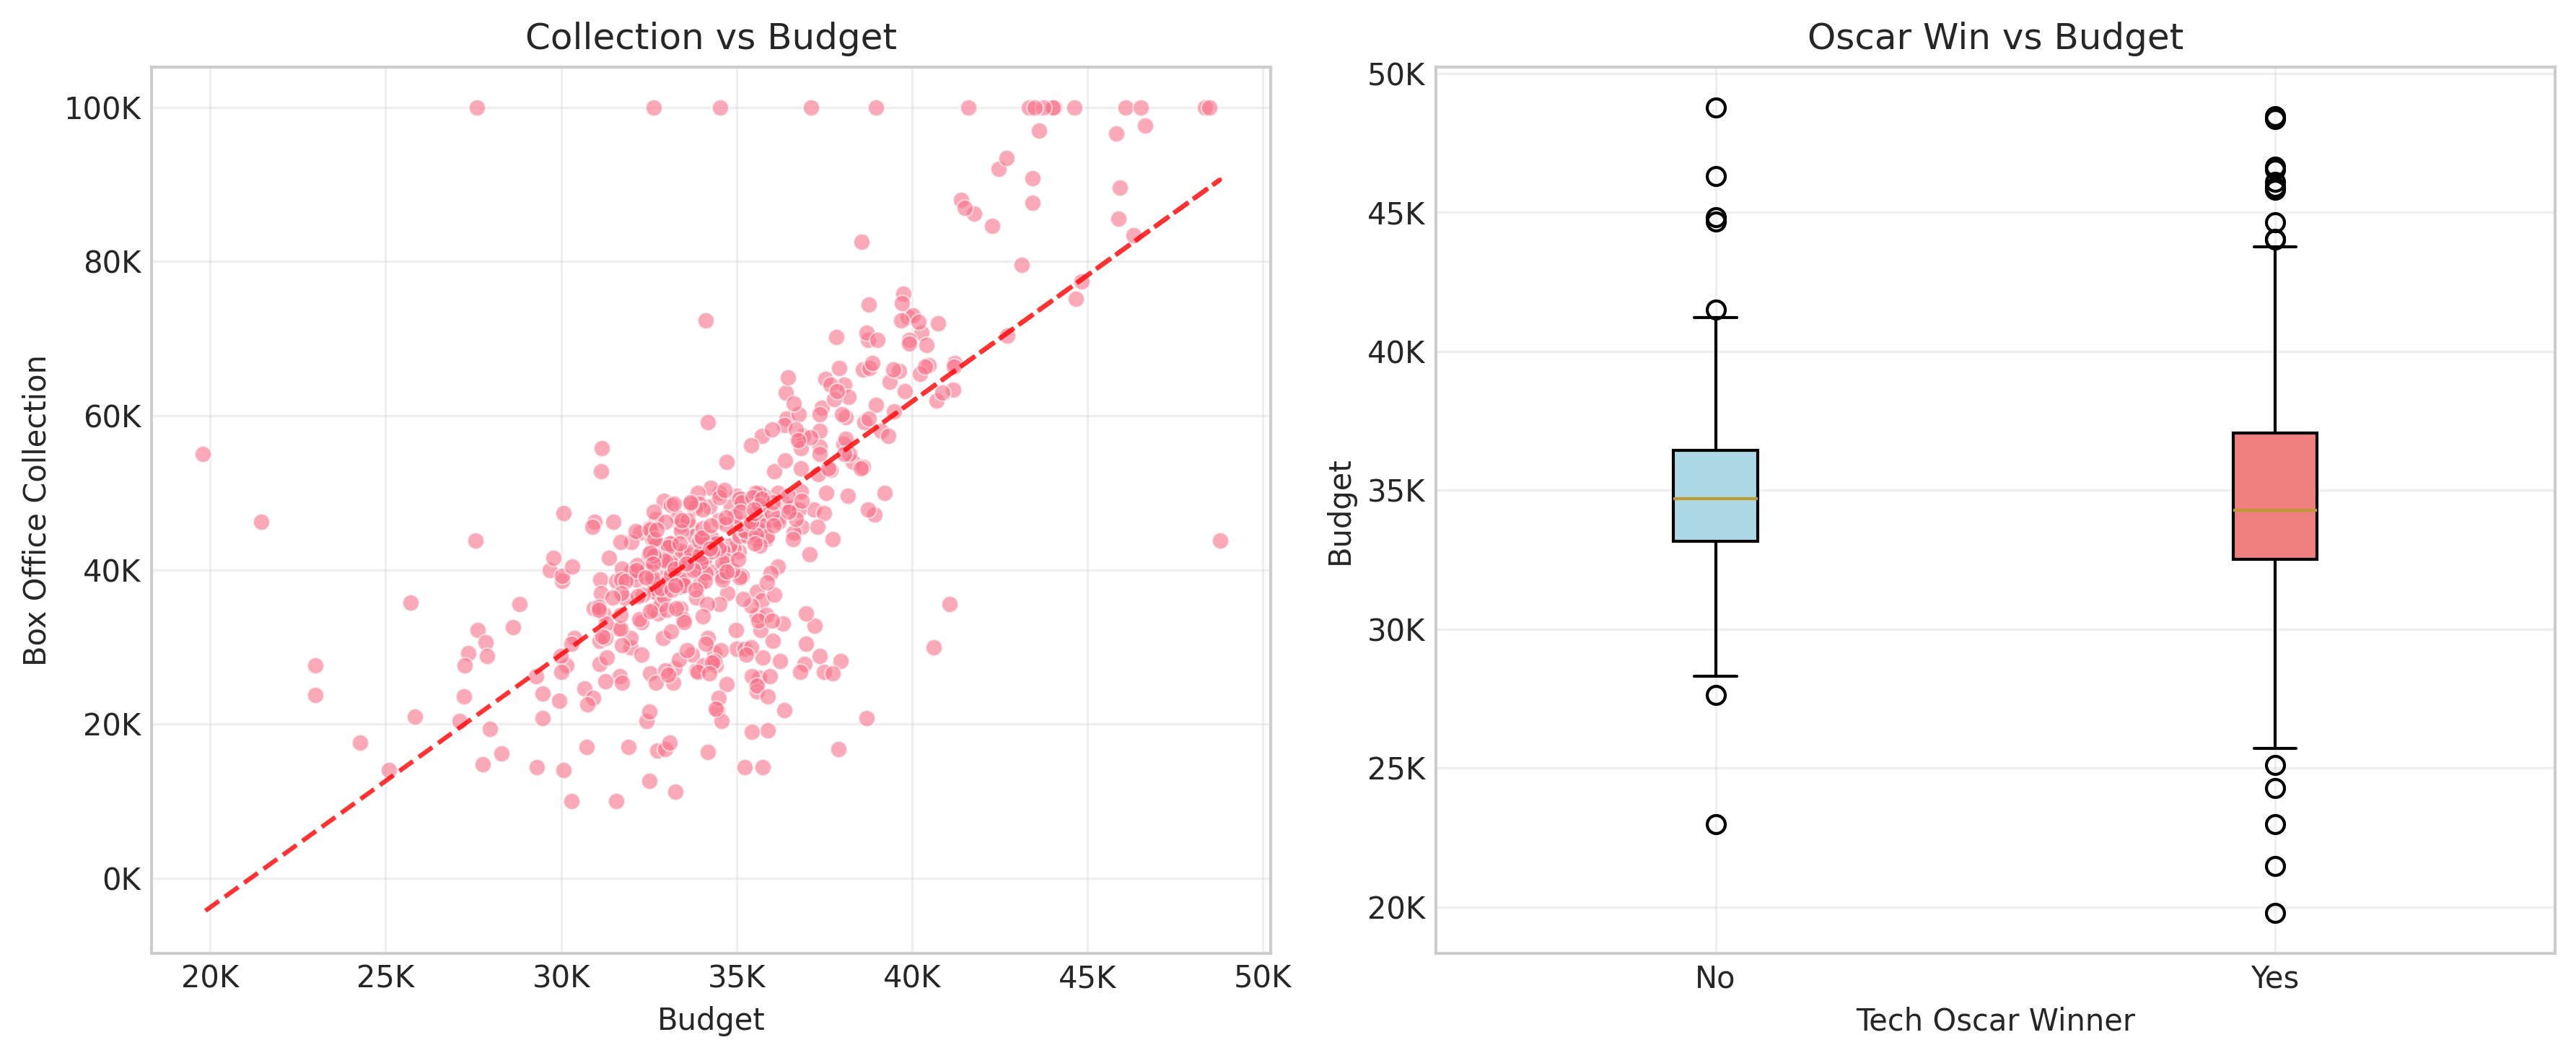
\includegraphics[width=0.9\textwidth]{../DatasetAnalysis/plots/Budget.png}
    \caption{Budget distribution}
\end{figure}
\begin{figure}
    \centering
    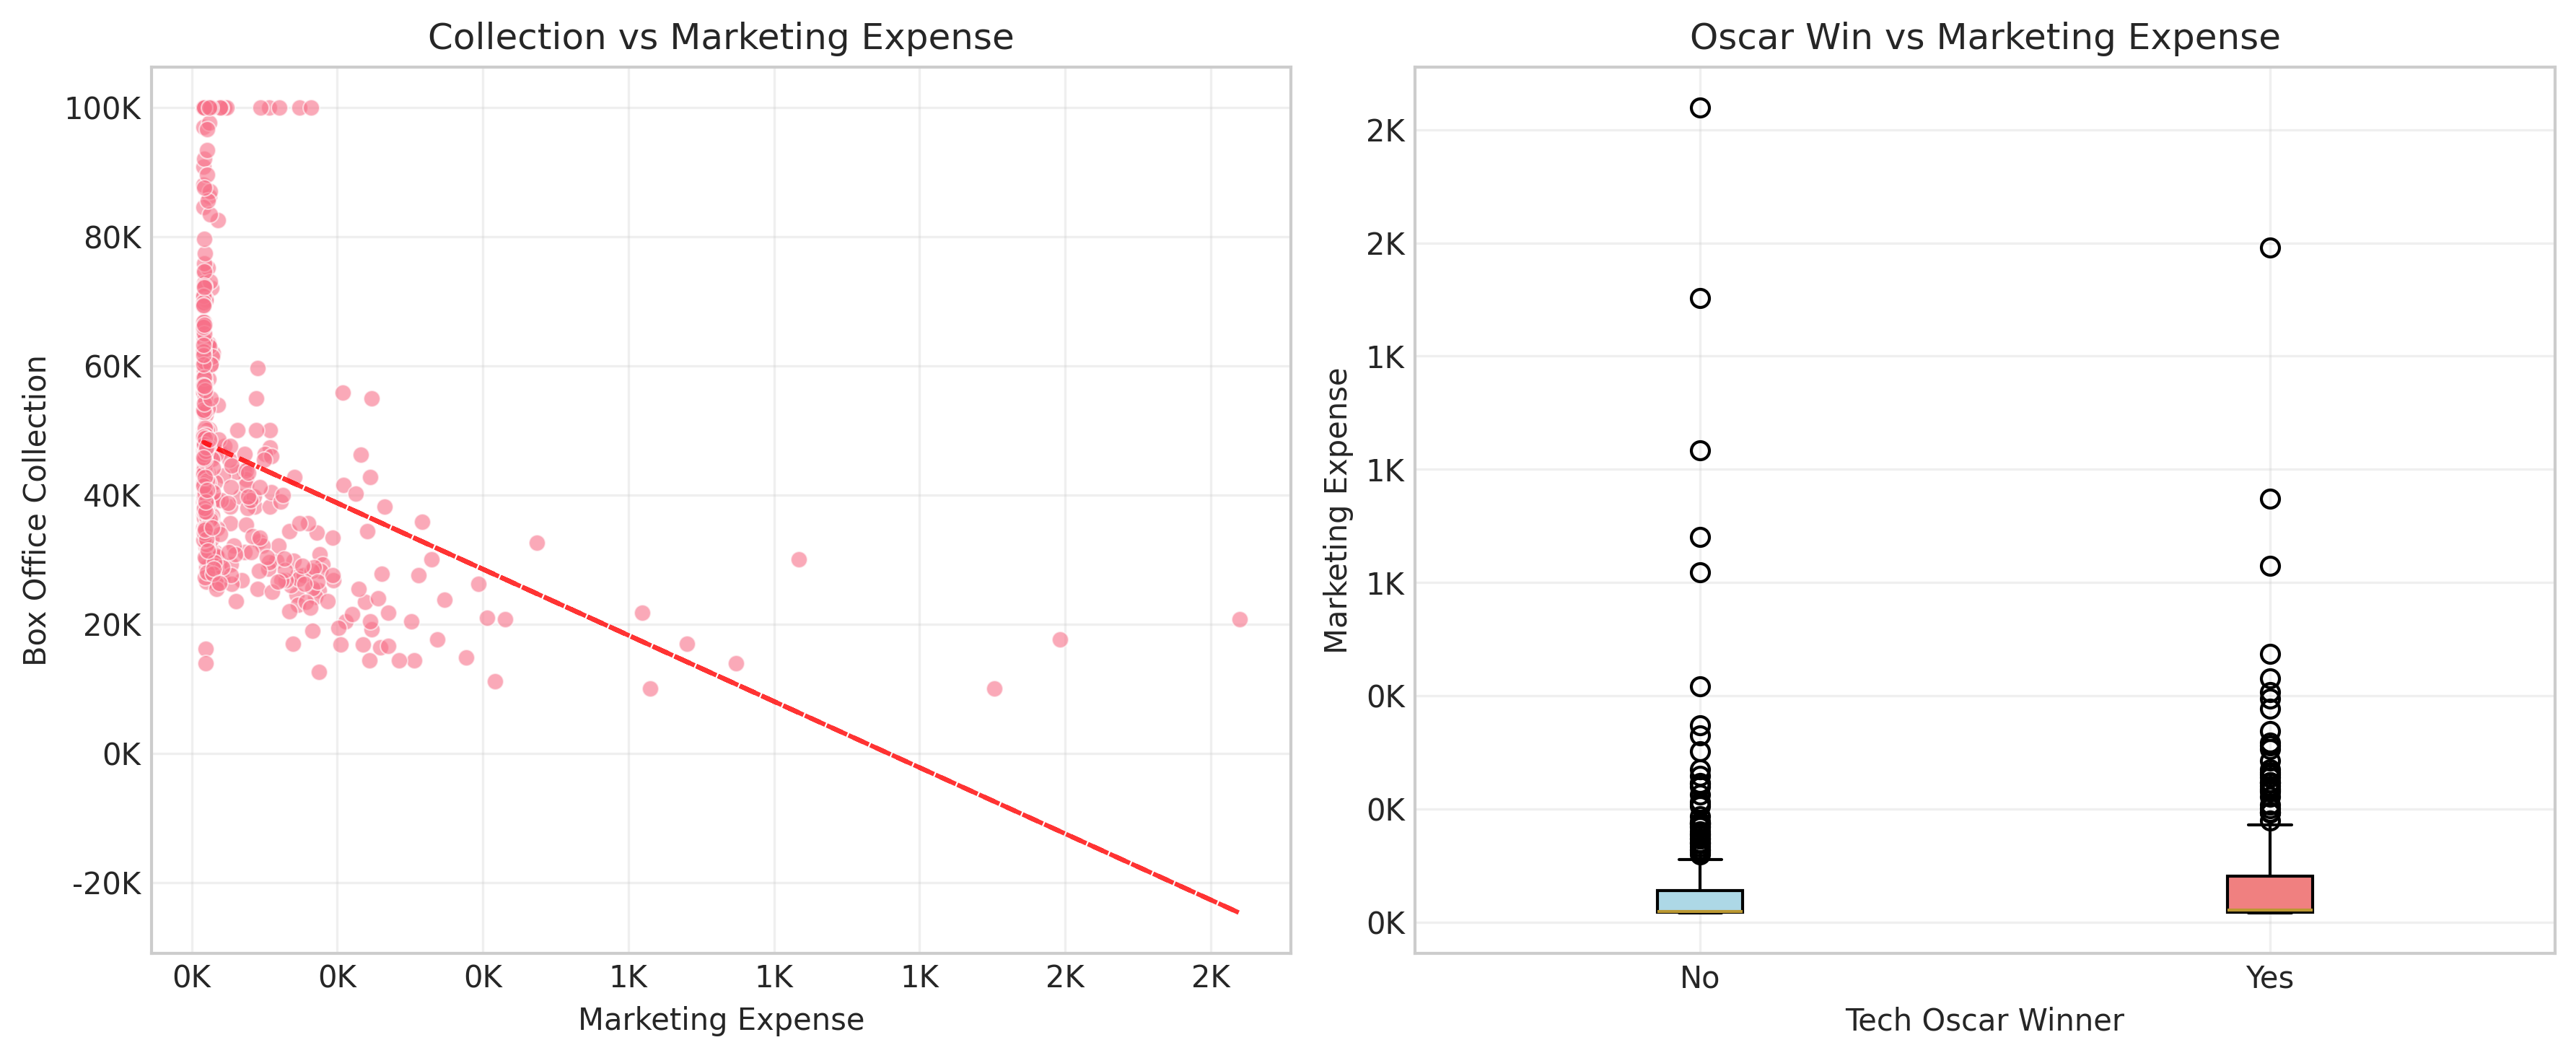
\includegraphics[width=0.9\textwidth]{../DatasetAnalysis/plots/Marketing_expense.png}
    \caption{Marketing expense distribution}
\end{figure}
\end{column}
\begin{column}{0.5\textwidth}
\begin{figure}
    \centering
    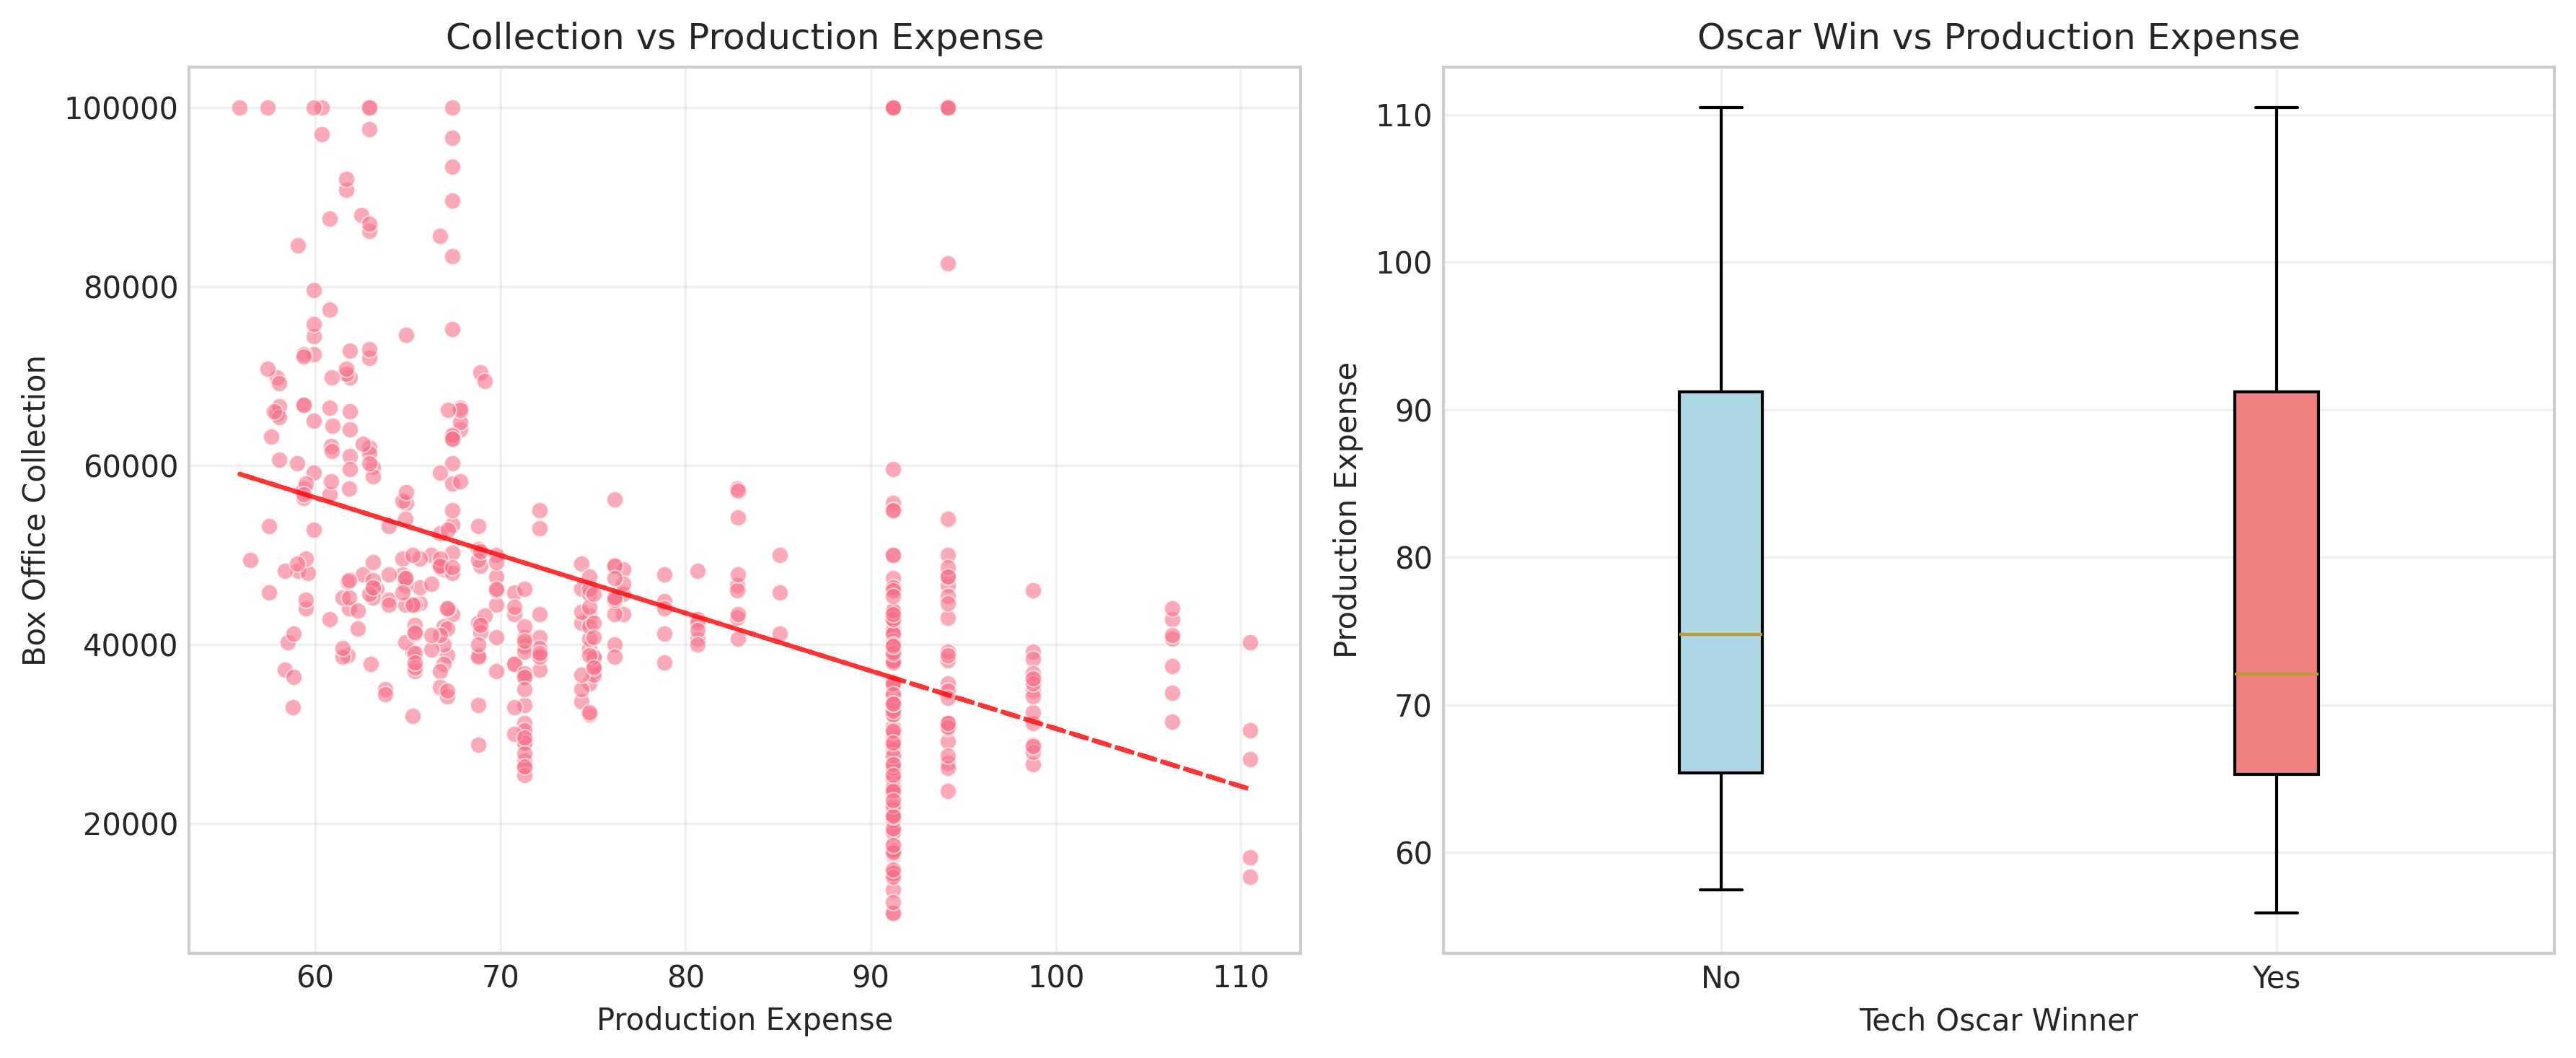
\includegraphics[width=0.9\textwidth]{../DatasetAnalysis/plots/Production_expense.png}
    \caption{Production expense distribution}
\end{figure}
\begin{figure}
    \centering
    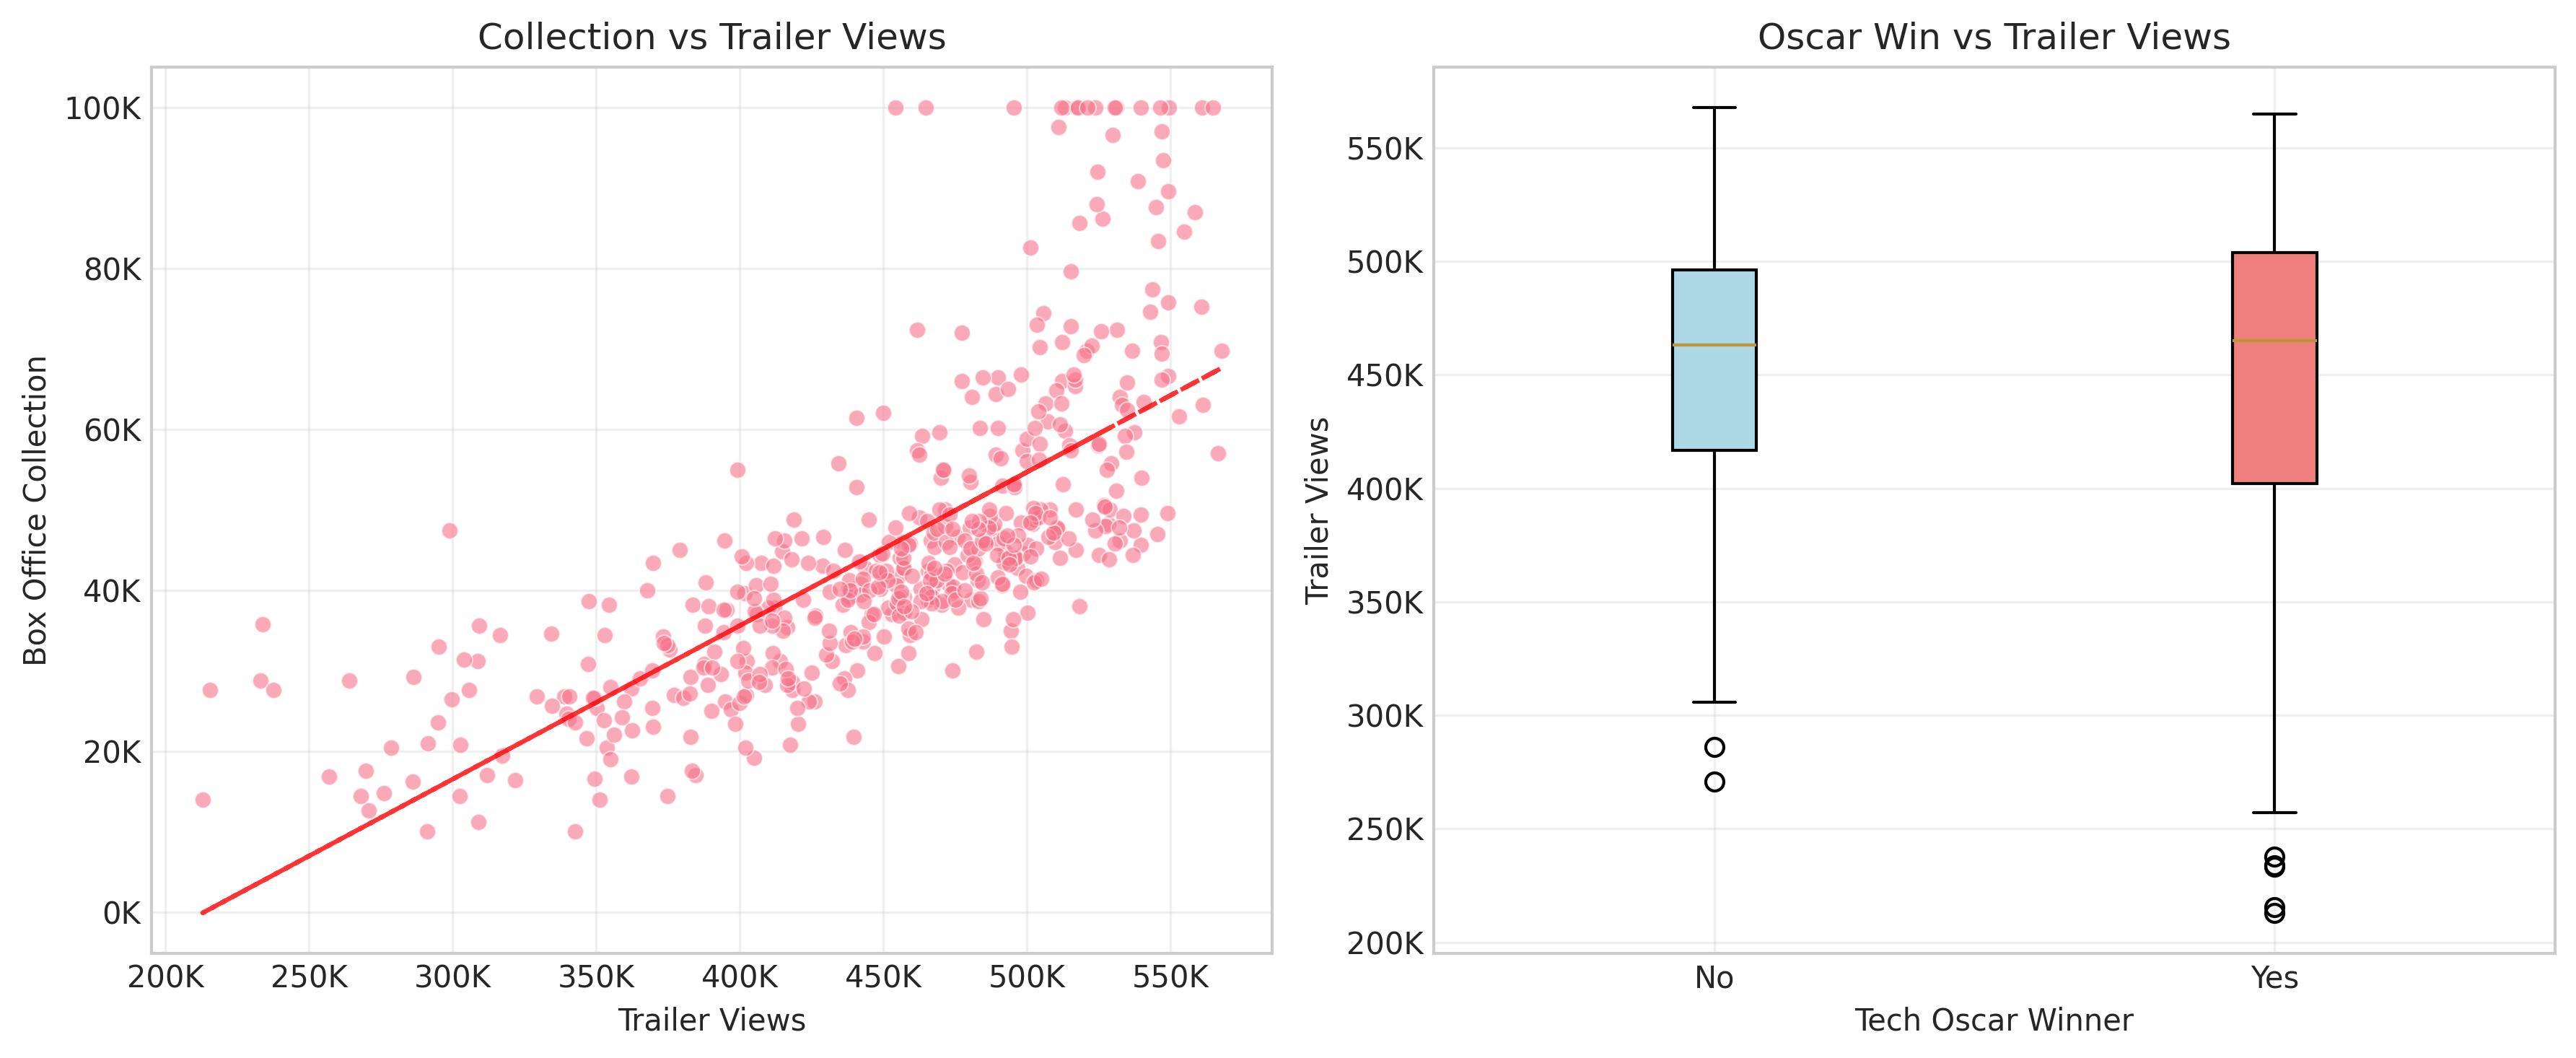
\includegraphics[width=0.9\textwidth]{../DatasetAnalysis/plots/Trailer_views.png}
    \caption{Trailer views distribution}
\end{figure}
\end{column}
\end{columns}
\end{frame}

\begin{frame}{Appendix: Feature Distributions - Ratings \& Reviews}
\begin{columns}
\begin{column}{0.5\textwidth}
\begin{figure}
    \centering
    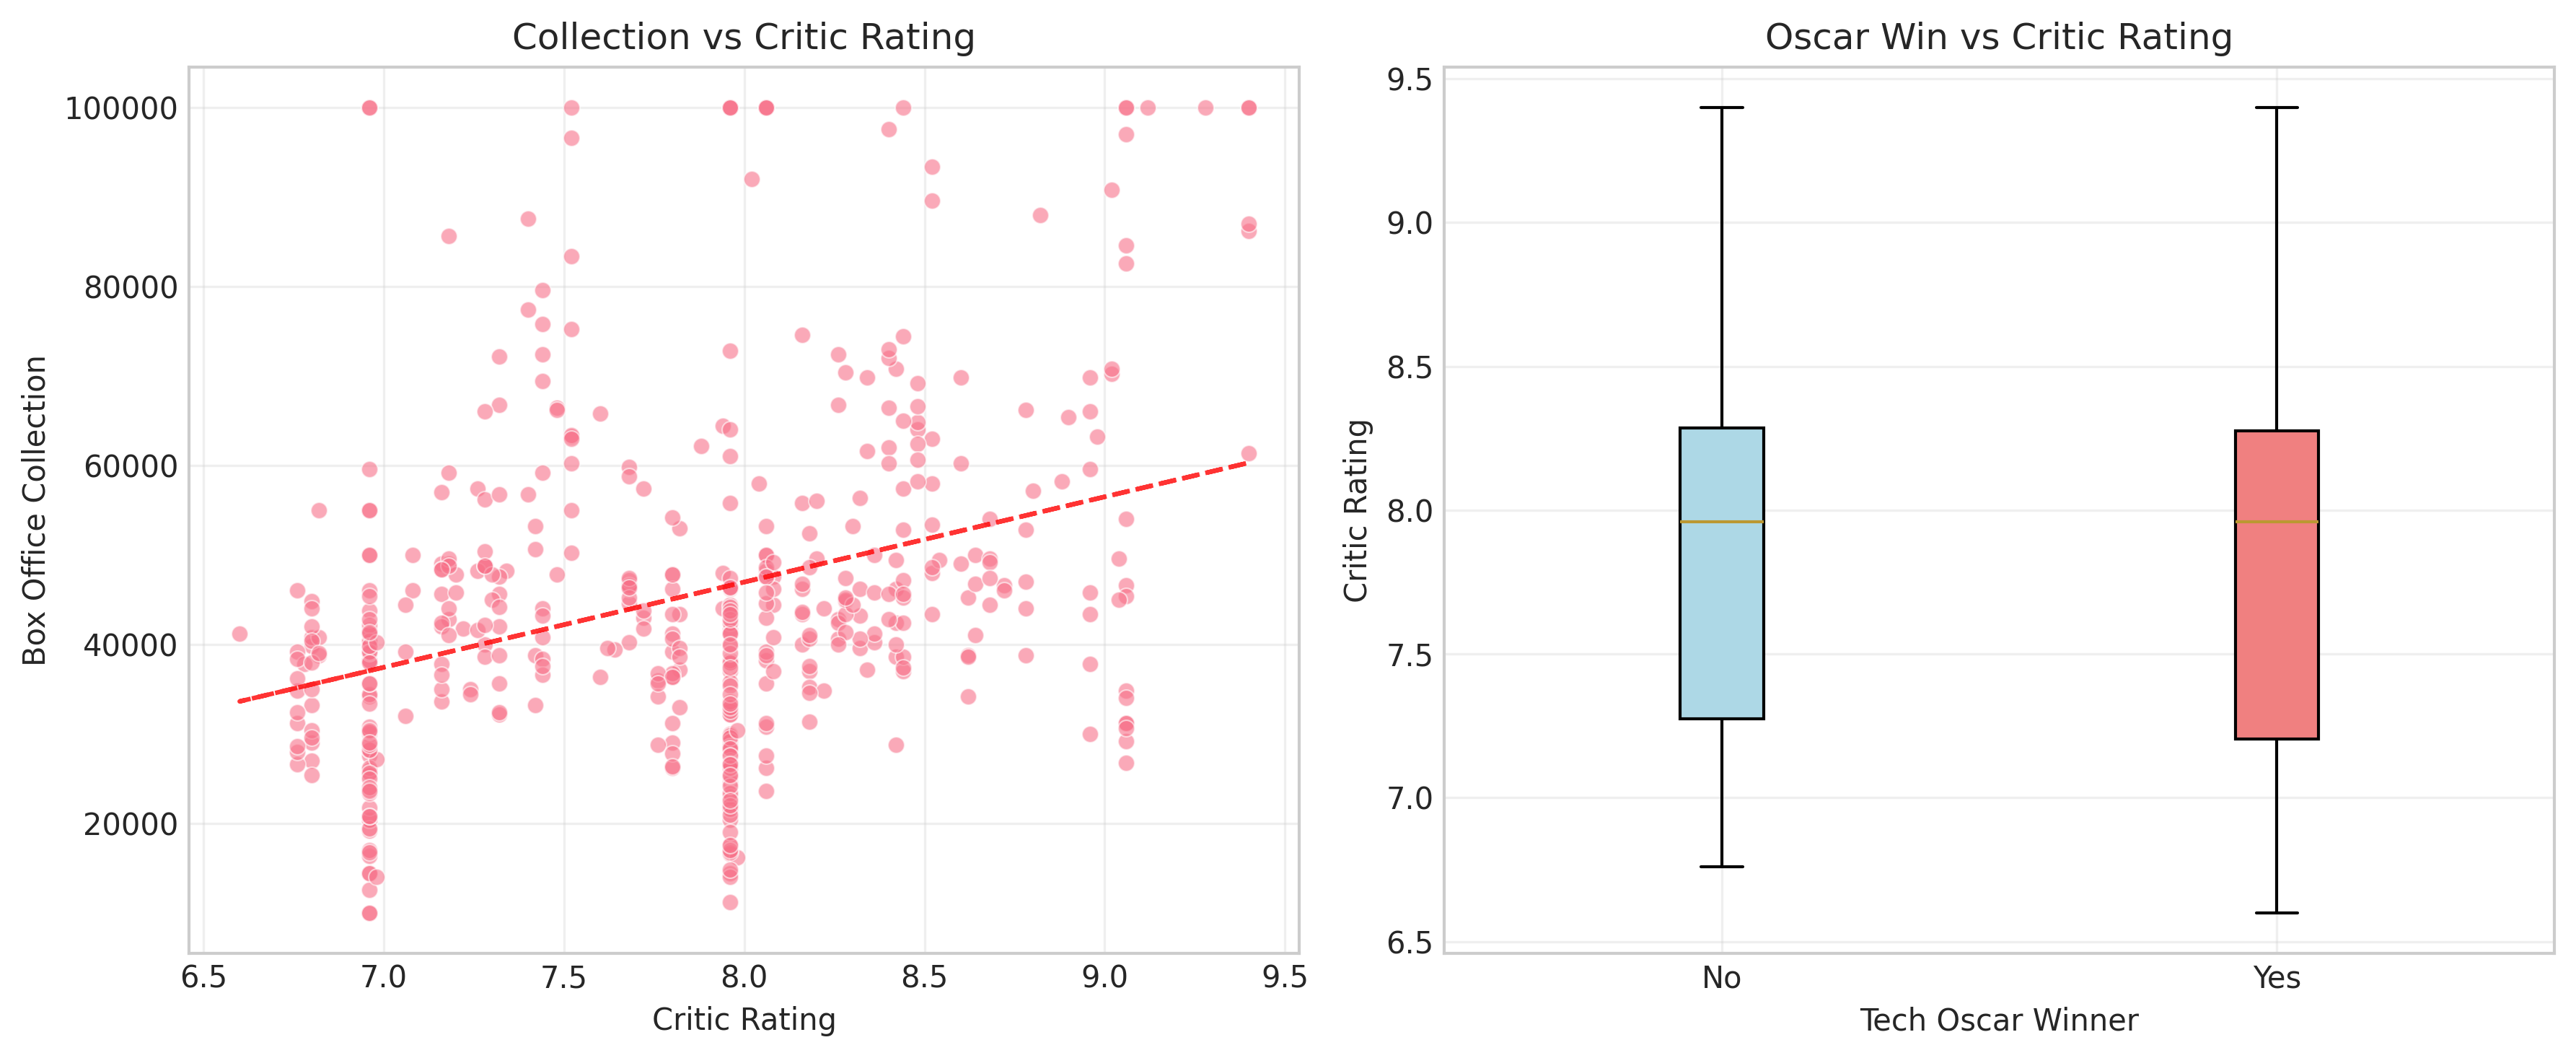
\includegraphics[width=0.9\textwidth]{../DatasetAnalysis/plots/Critic_rating.png}
    \caption{Critic rating distribution}
\end{figure}
\begin{figure}
    \centering
    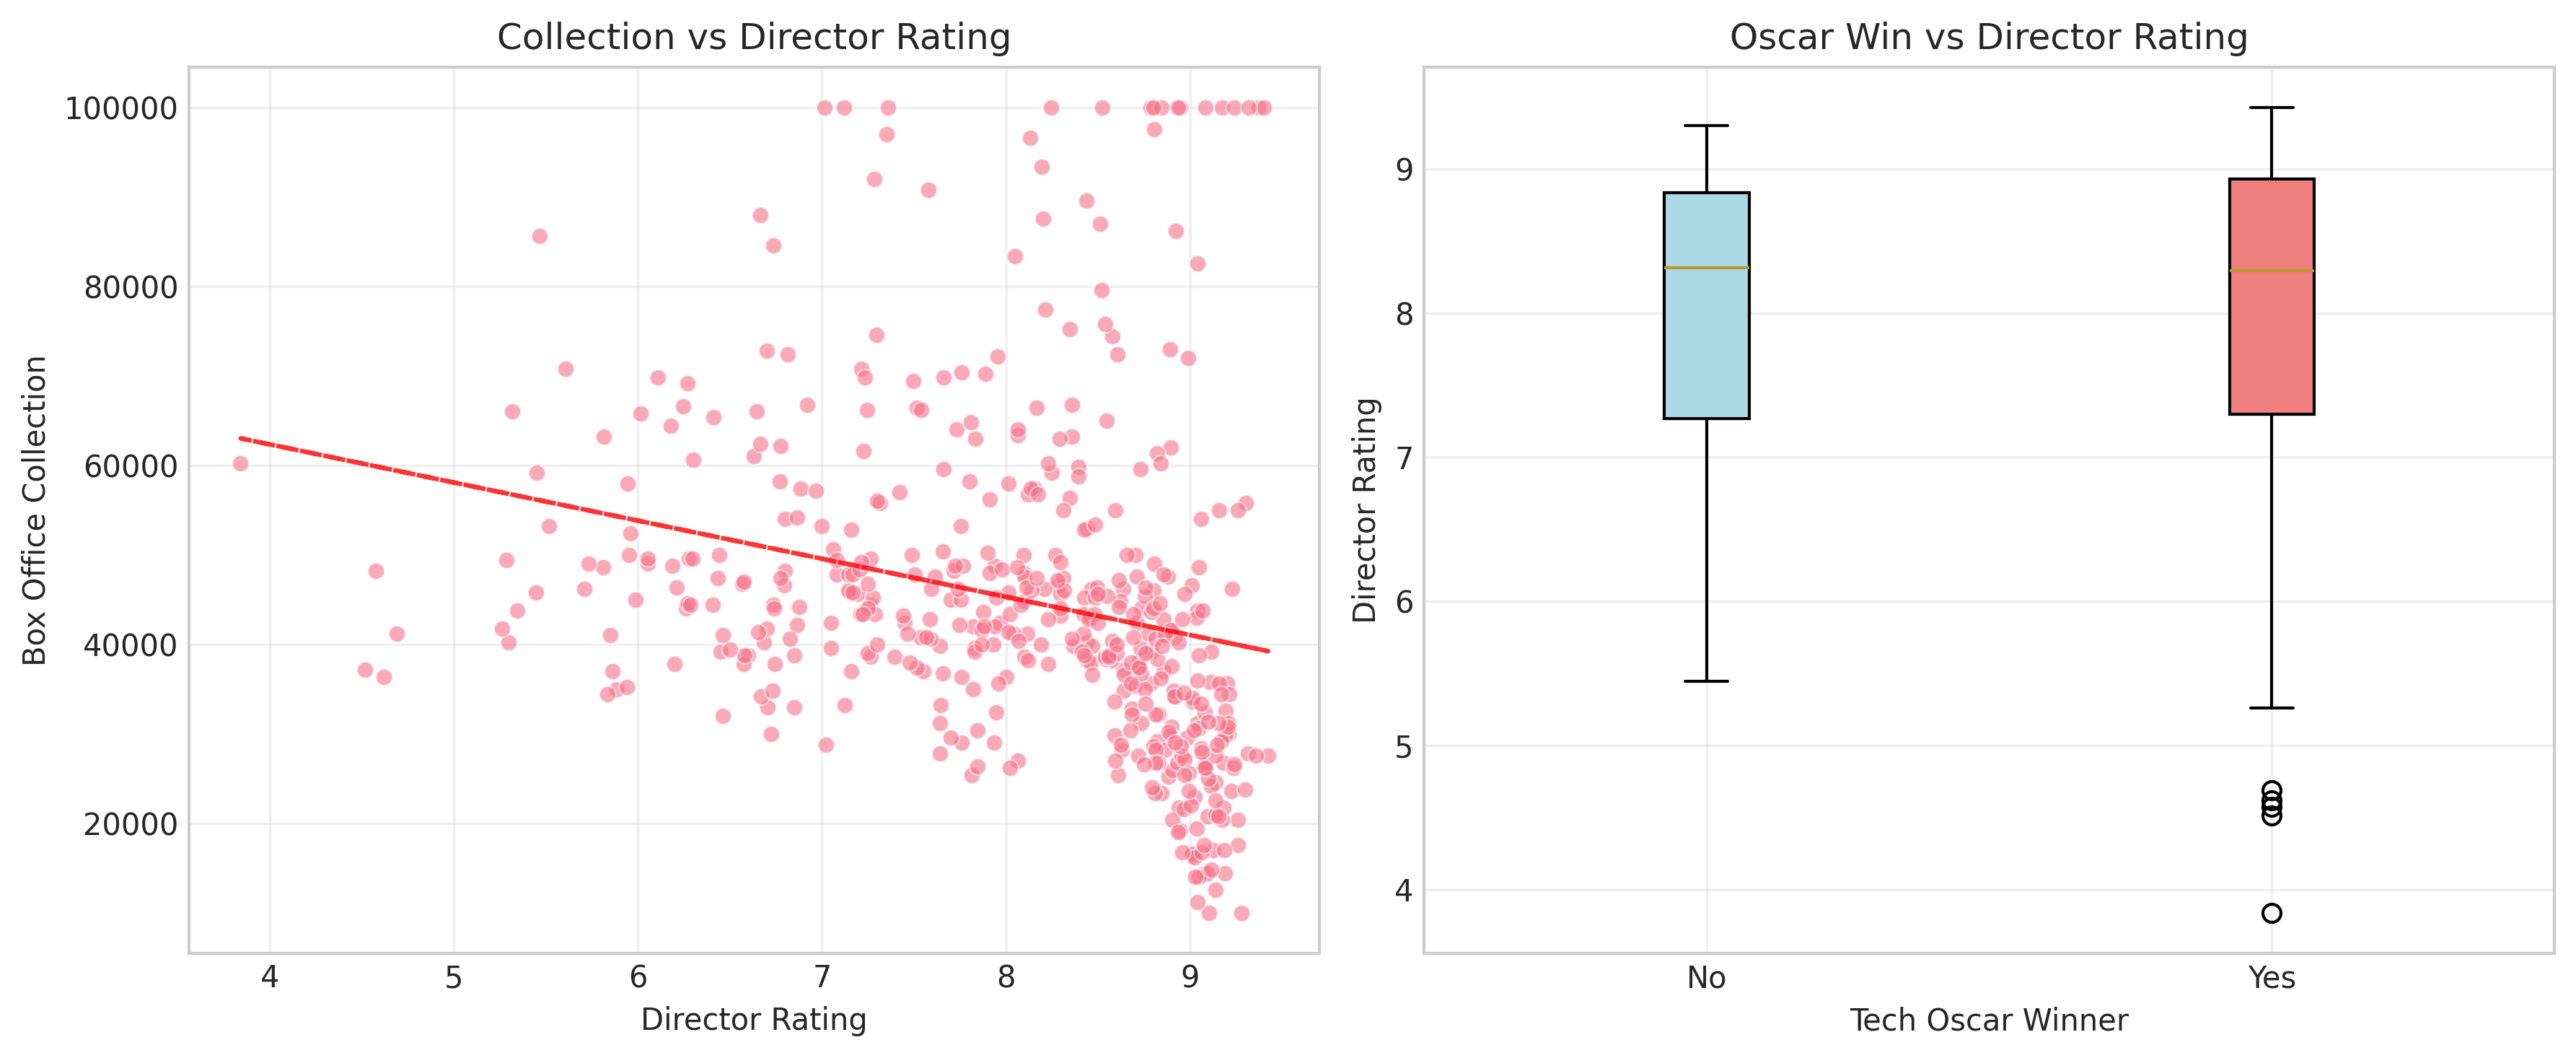
\includegraphics[width=0.9\textwidth]{../DatasetAnalysis/plots/Director_rating.png}
    \caption{Director rating distribution}
\end{figure}
\end{column}
\begin{column}{0.5\textwidth}
\begin{figure}
    \centering
    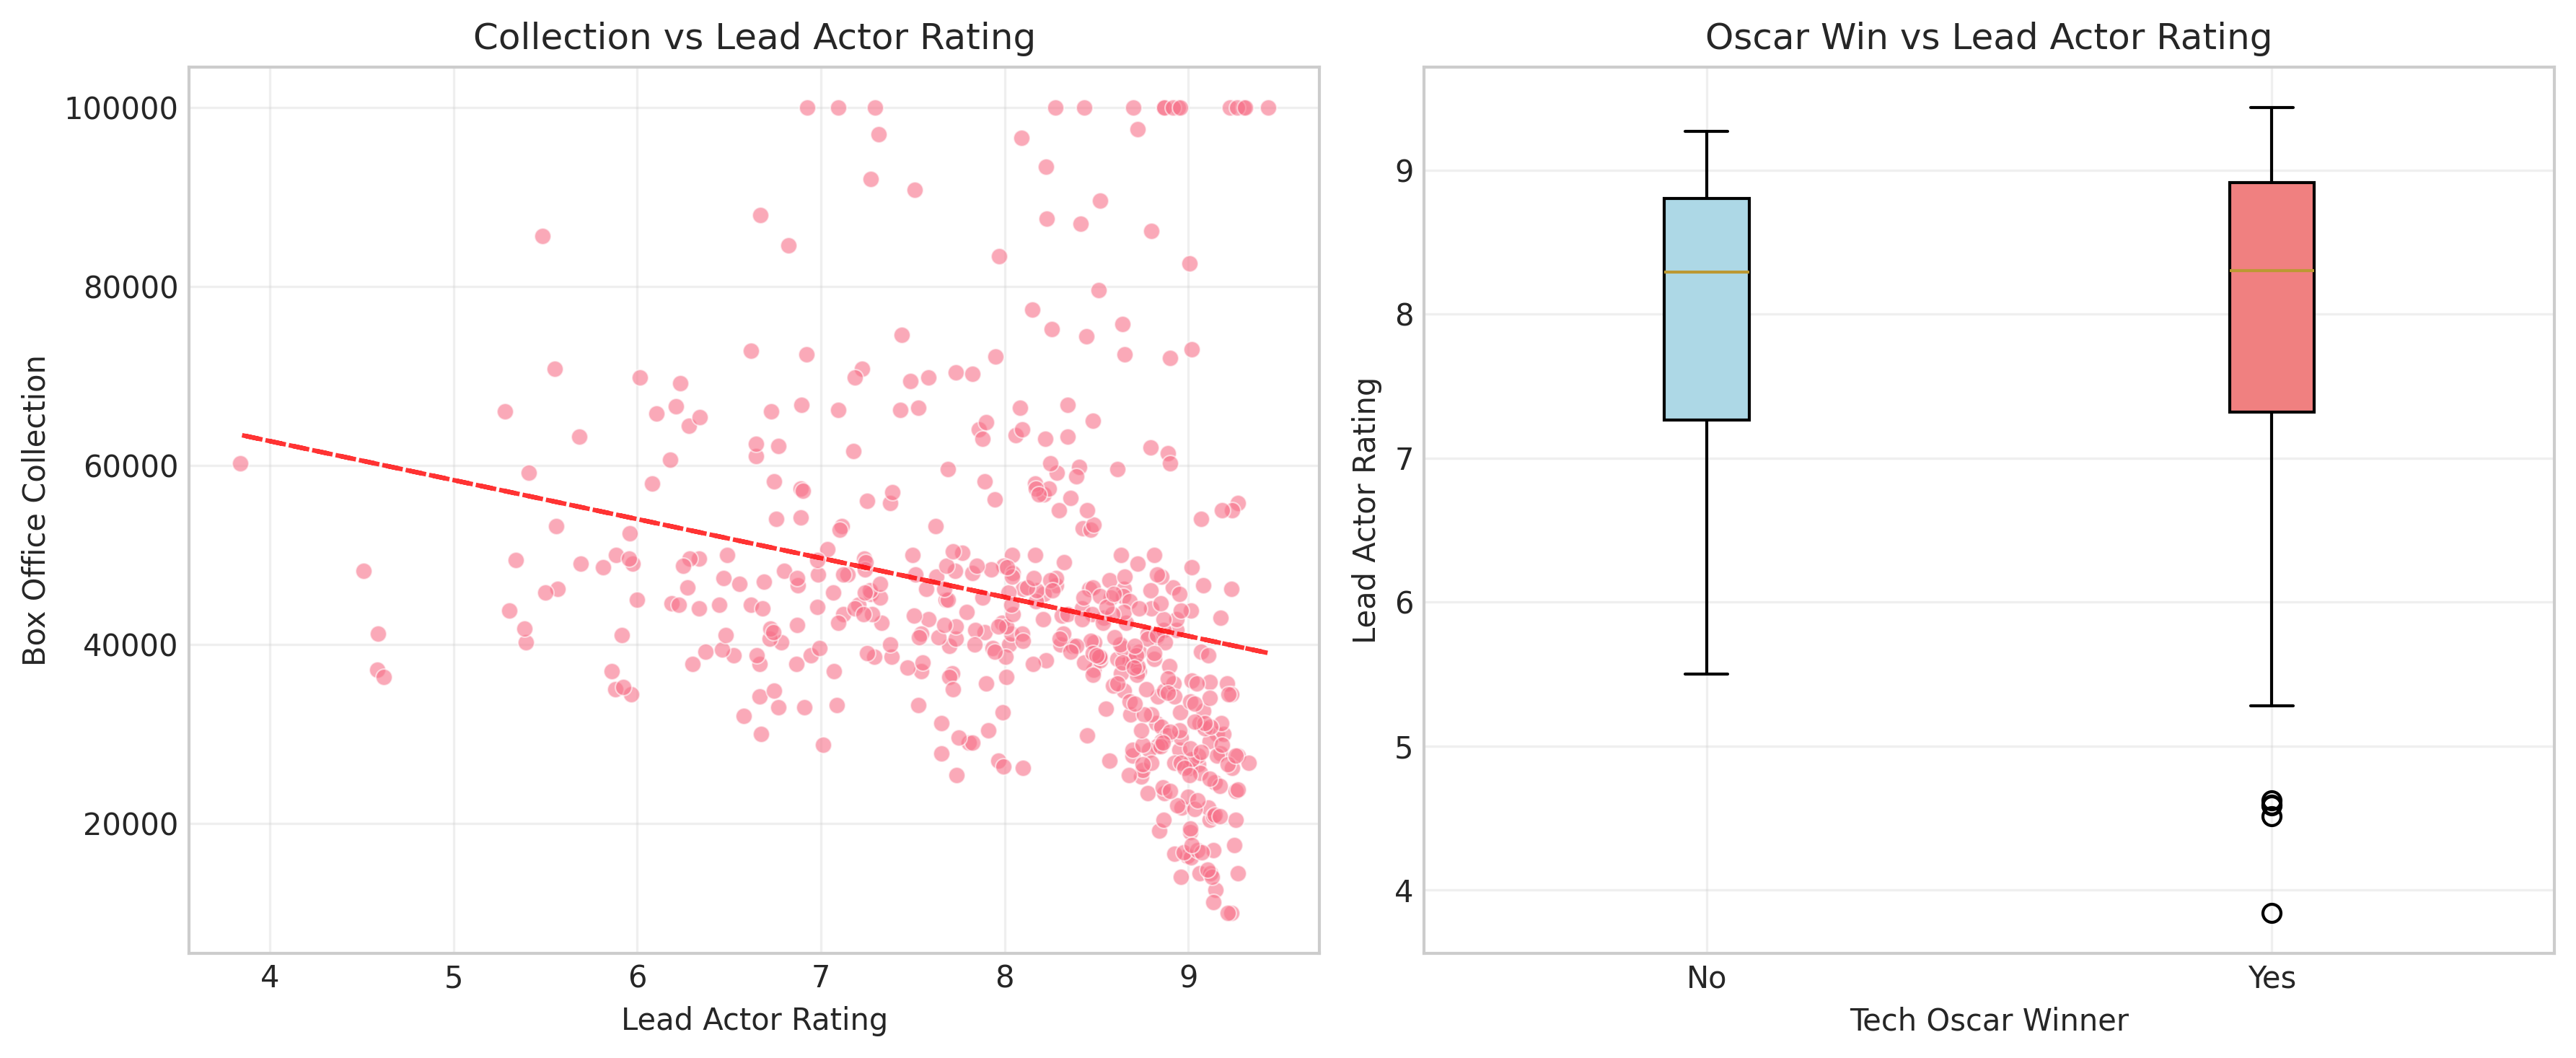
\includegraphics[width=0.9\textwidth]{../DatasetAnalysis/plots/Lead__Actor_Rating.png}
    \caption{Lead Actor rating distribution}
\end{figure}
\begin{figure}
    \centering
    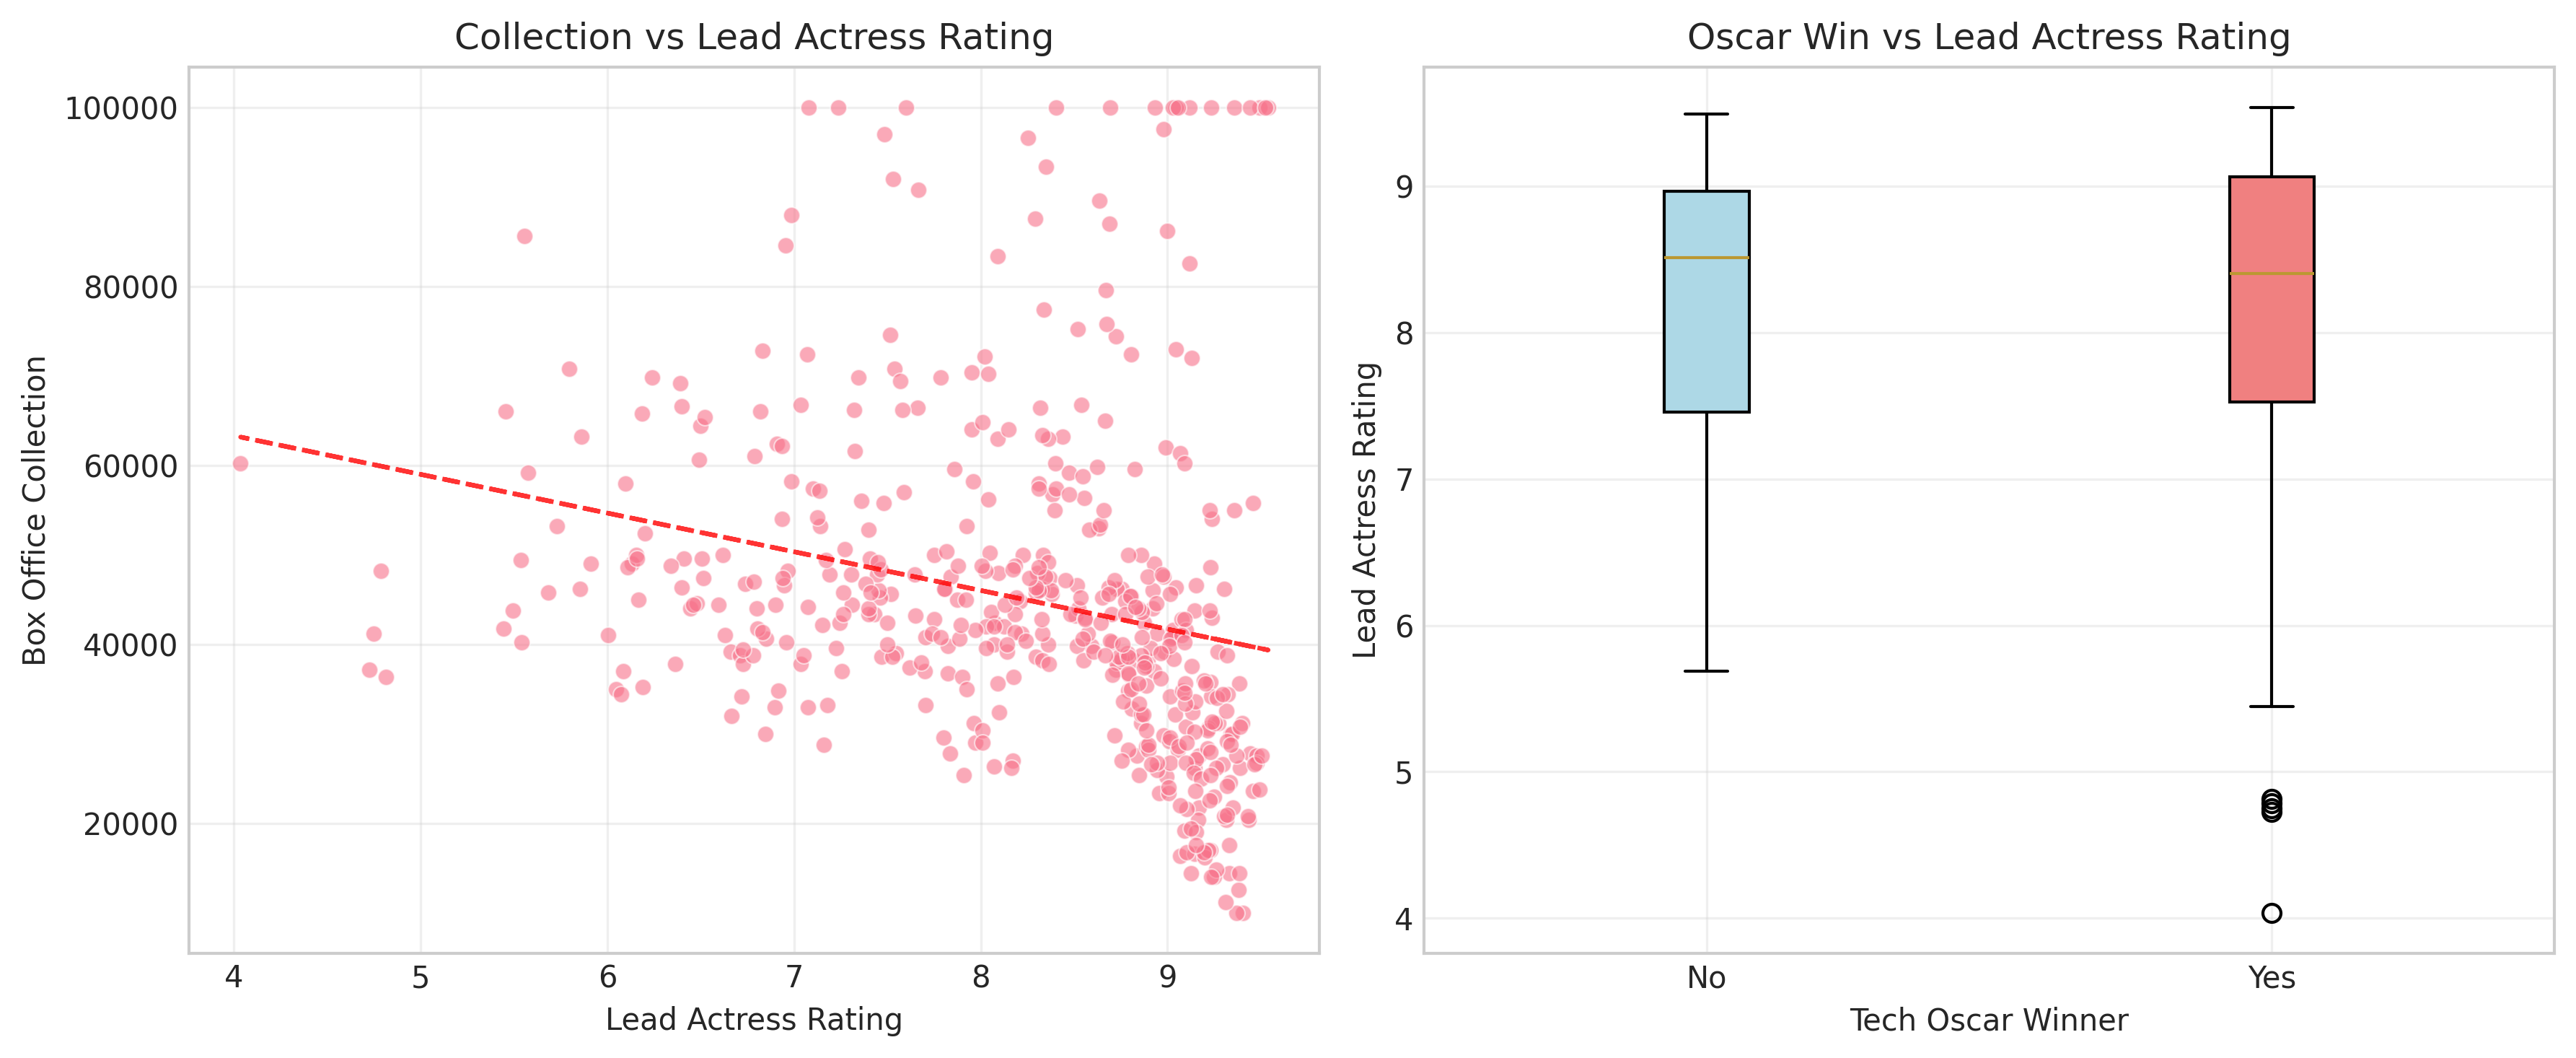
\includegraphics[width=0.9\textwidth]{../DatasetAnalysis/plots/Lead_Actress_rating.png}
    \caption{Lead Actress rating distribution}
\end{figure}
\end{column}
\end{columns}
\end{frame}

\begin{frame}{Appendix: Feature Distributions - Production Metrics}
\begin{columns}
\begin{column}{0.5\textwidth}
\begin{figure}
    \centering
    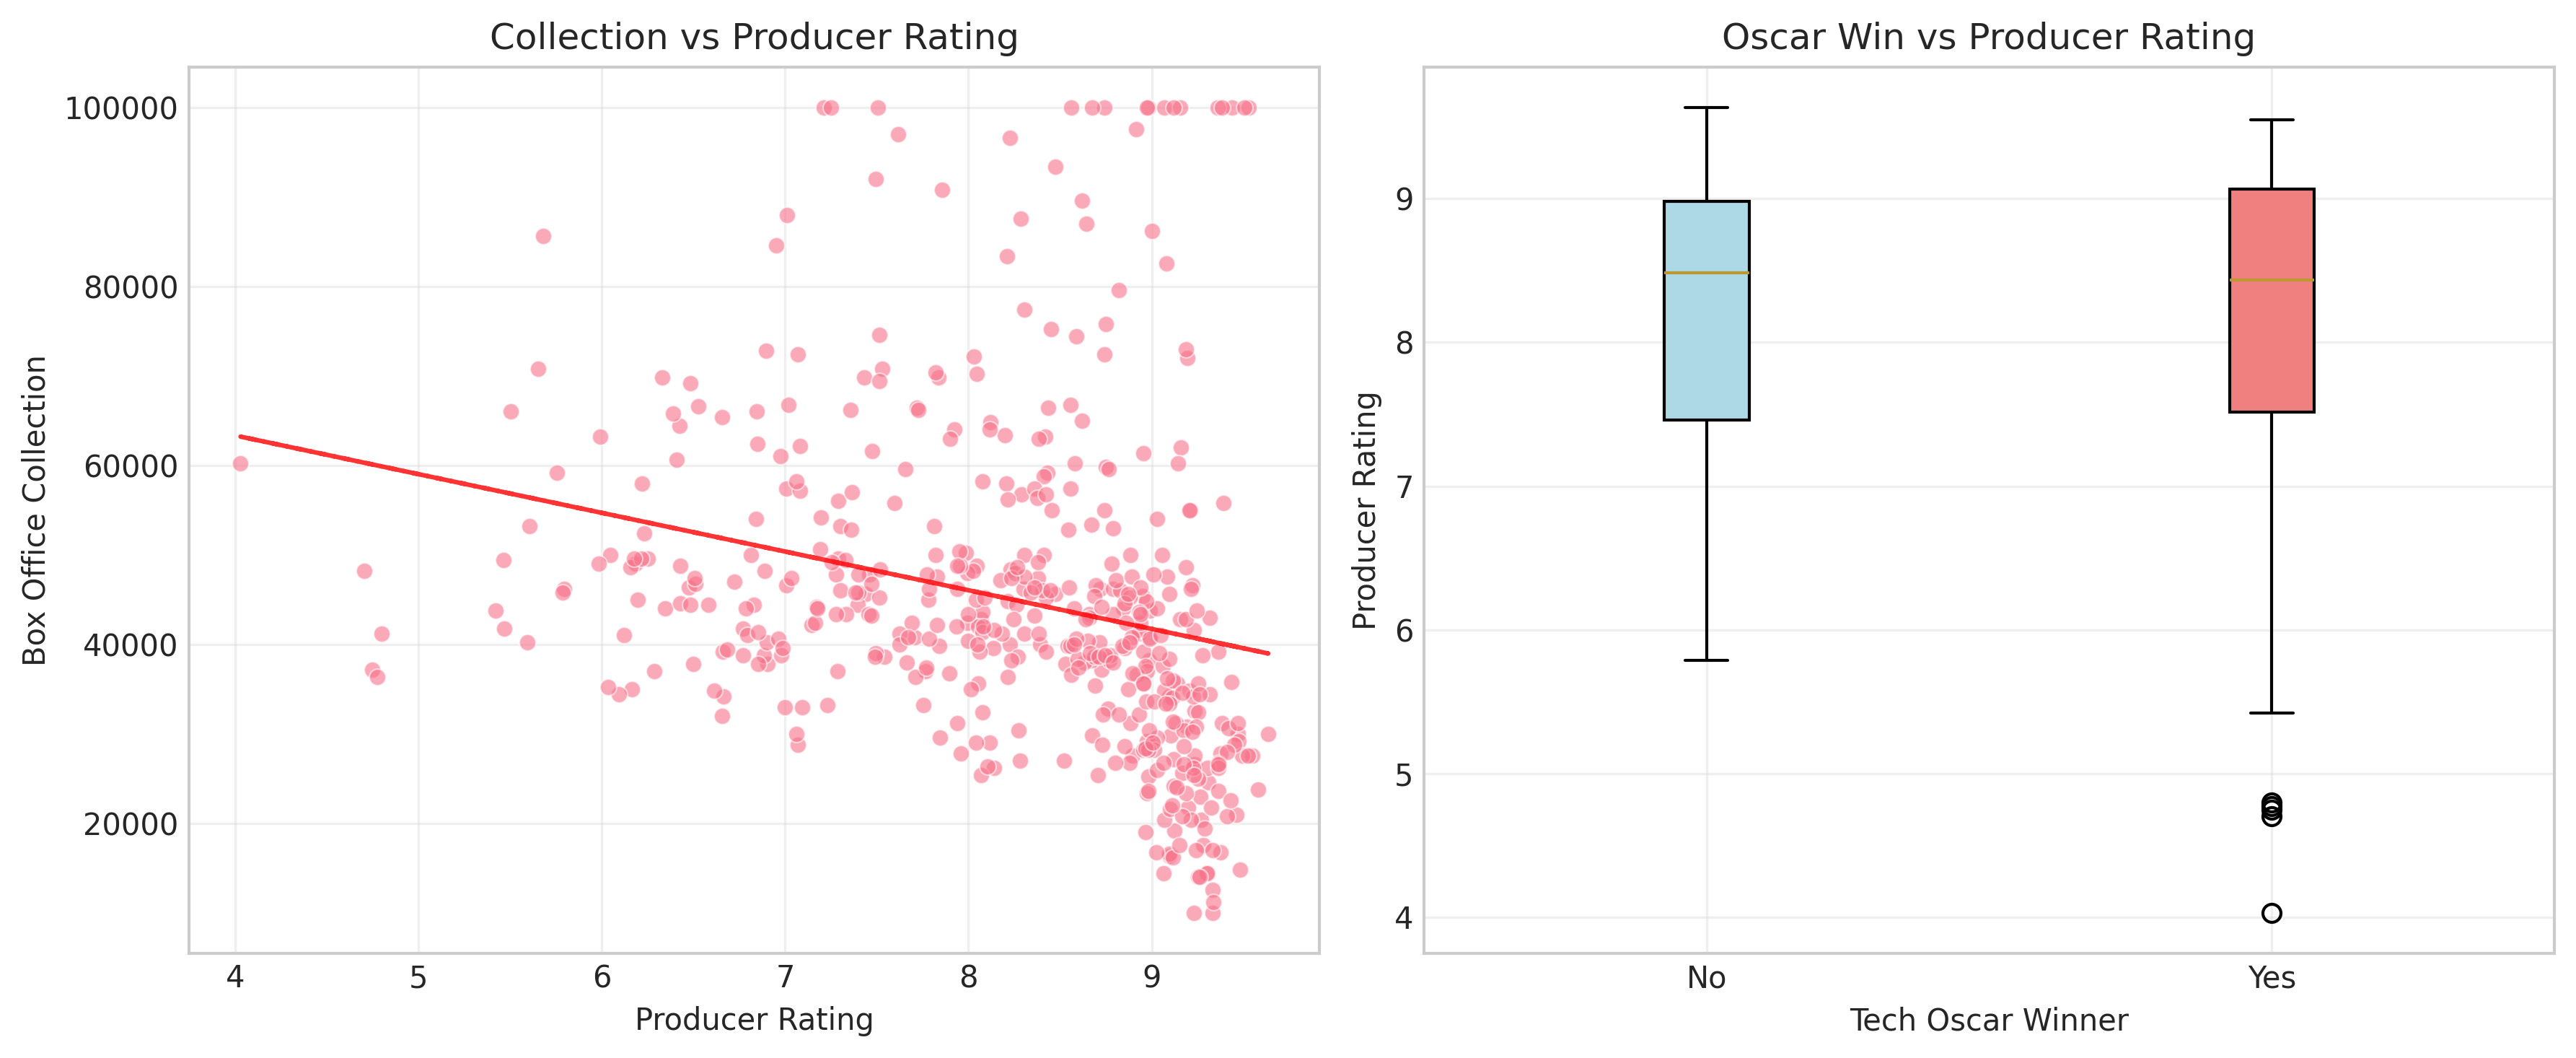
\includegraphics[width=0.9\textwidth]{../DatasetAnalysis/plots/Producer_rating.png}
    \caption{Producer rating distribution}
\end{figure}
\begin{figure}
    \centering
    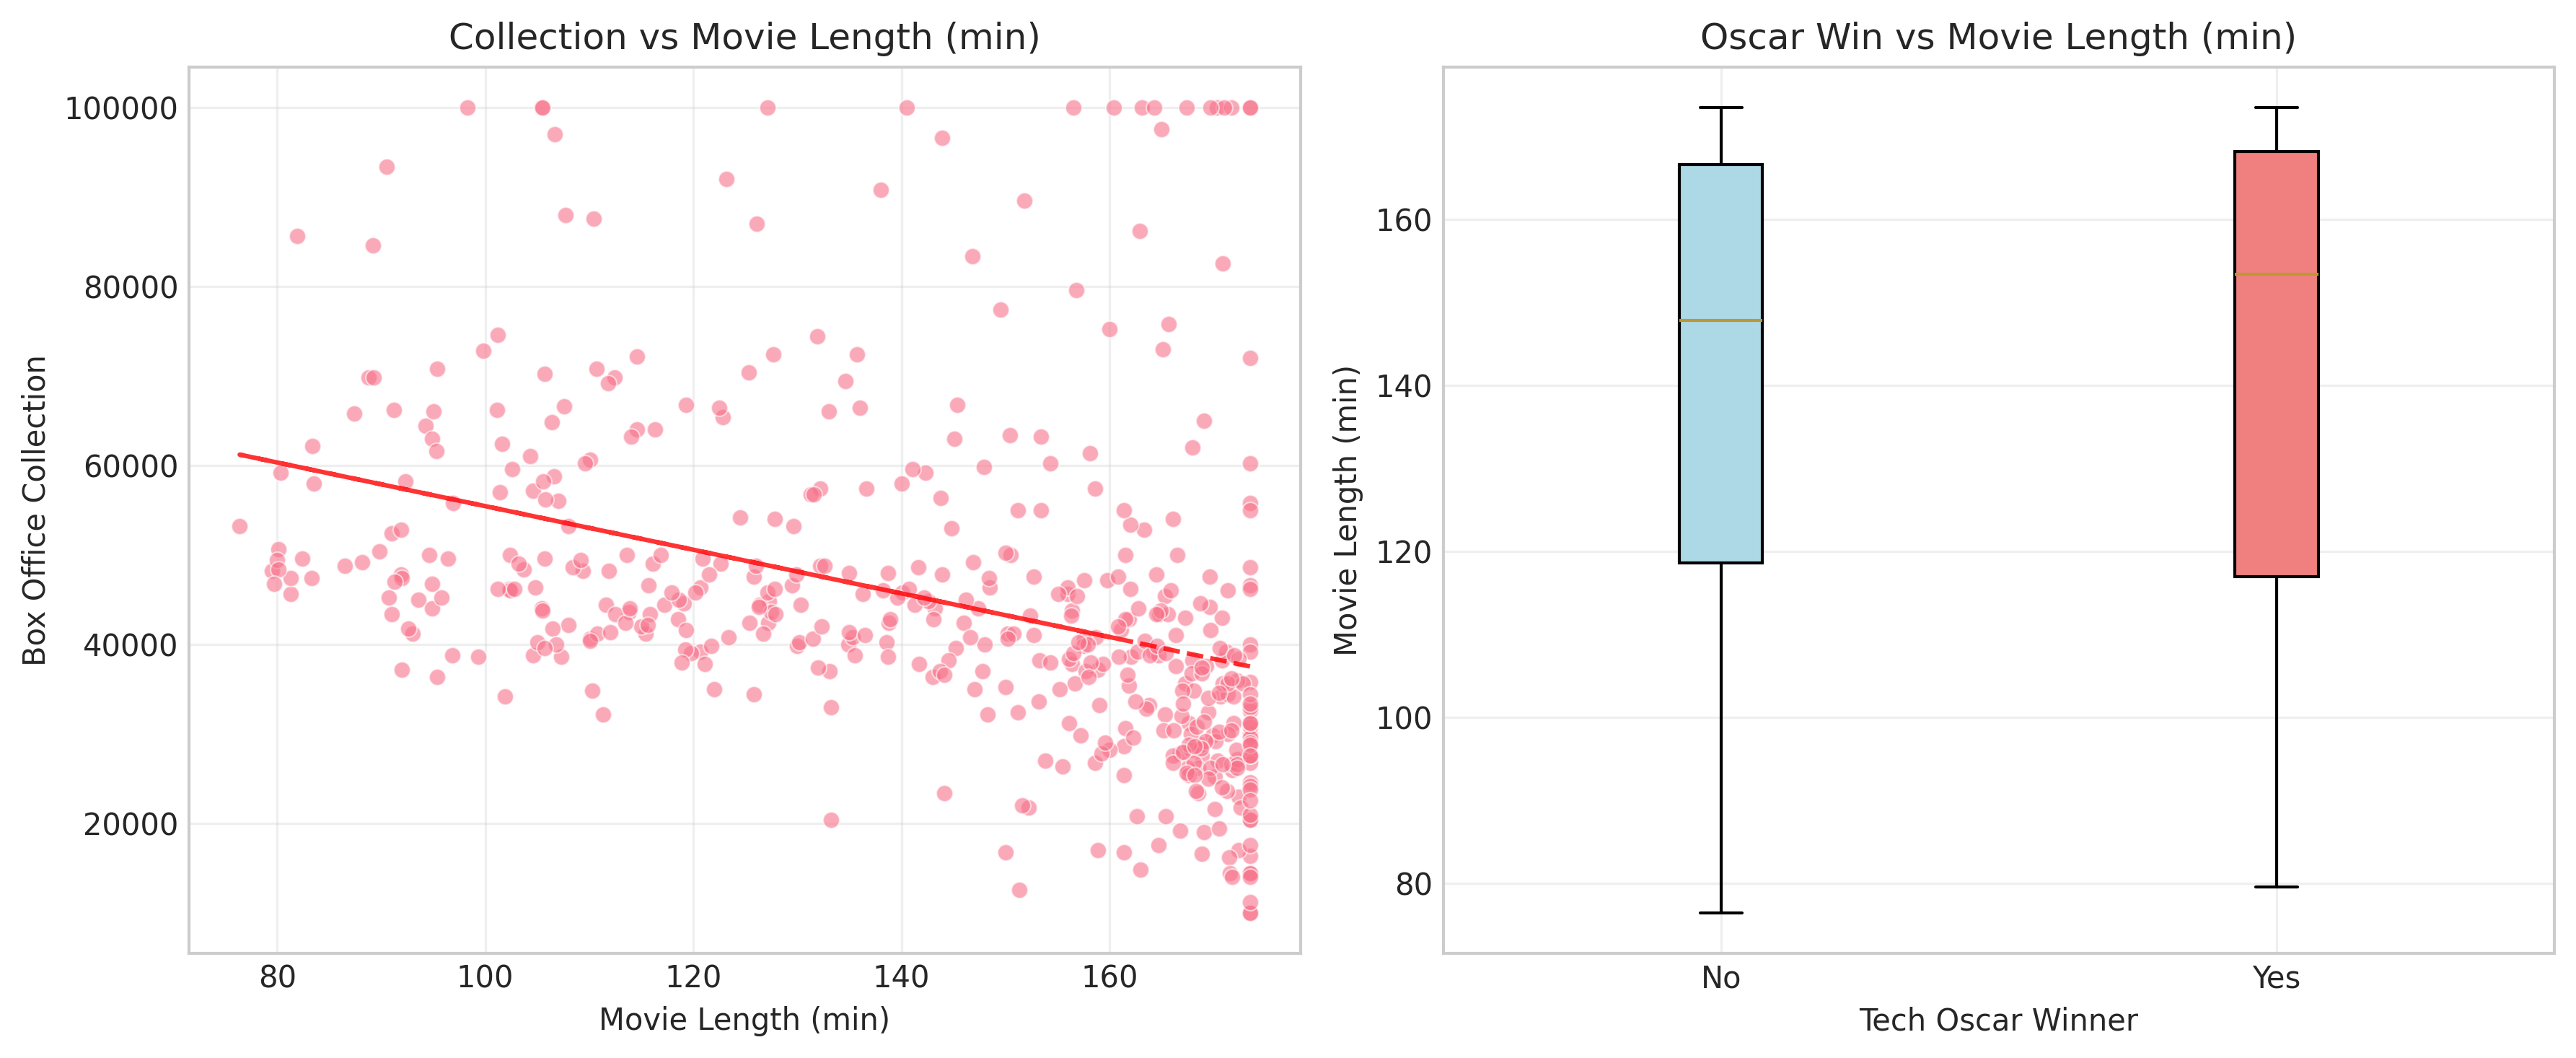
\includegraphics[width=0.9\textwidth]{../DatasetAnalysis/plots/Movie_length.png}
    \caption{Movie length distribution}
\end{figure}
\end{column}
\begin{column}{0.5\textwidth}
\begin{figure}
    \centering
    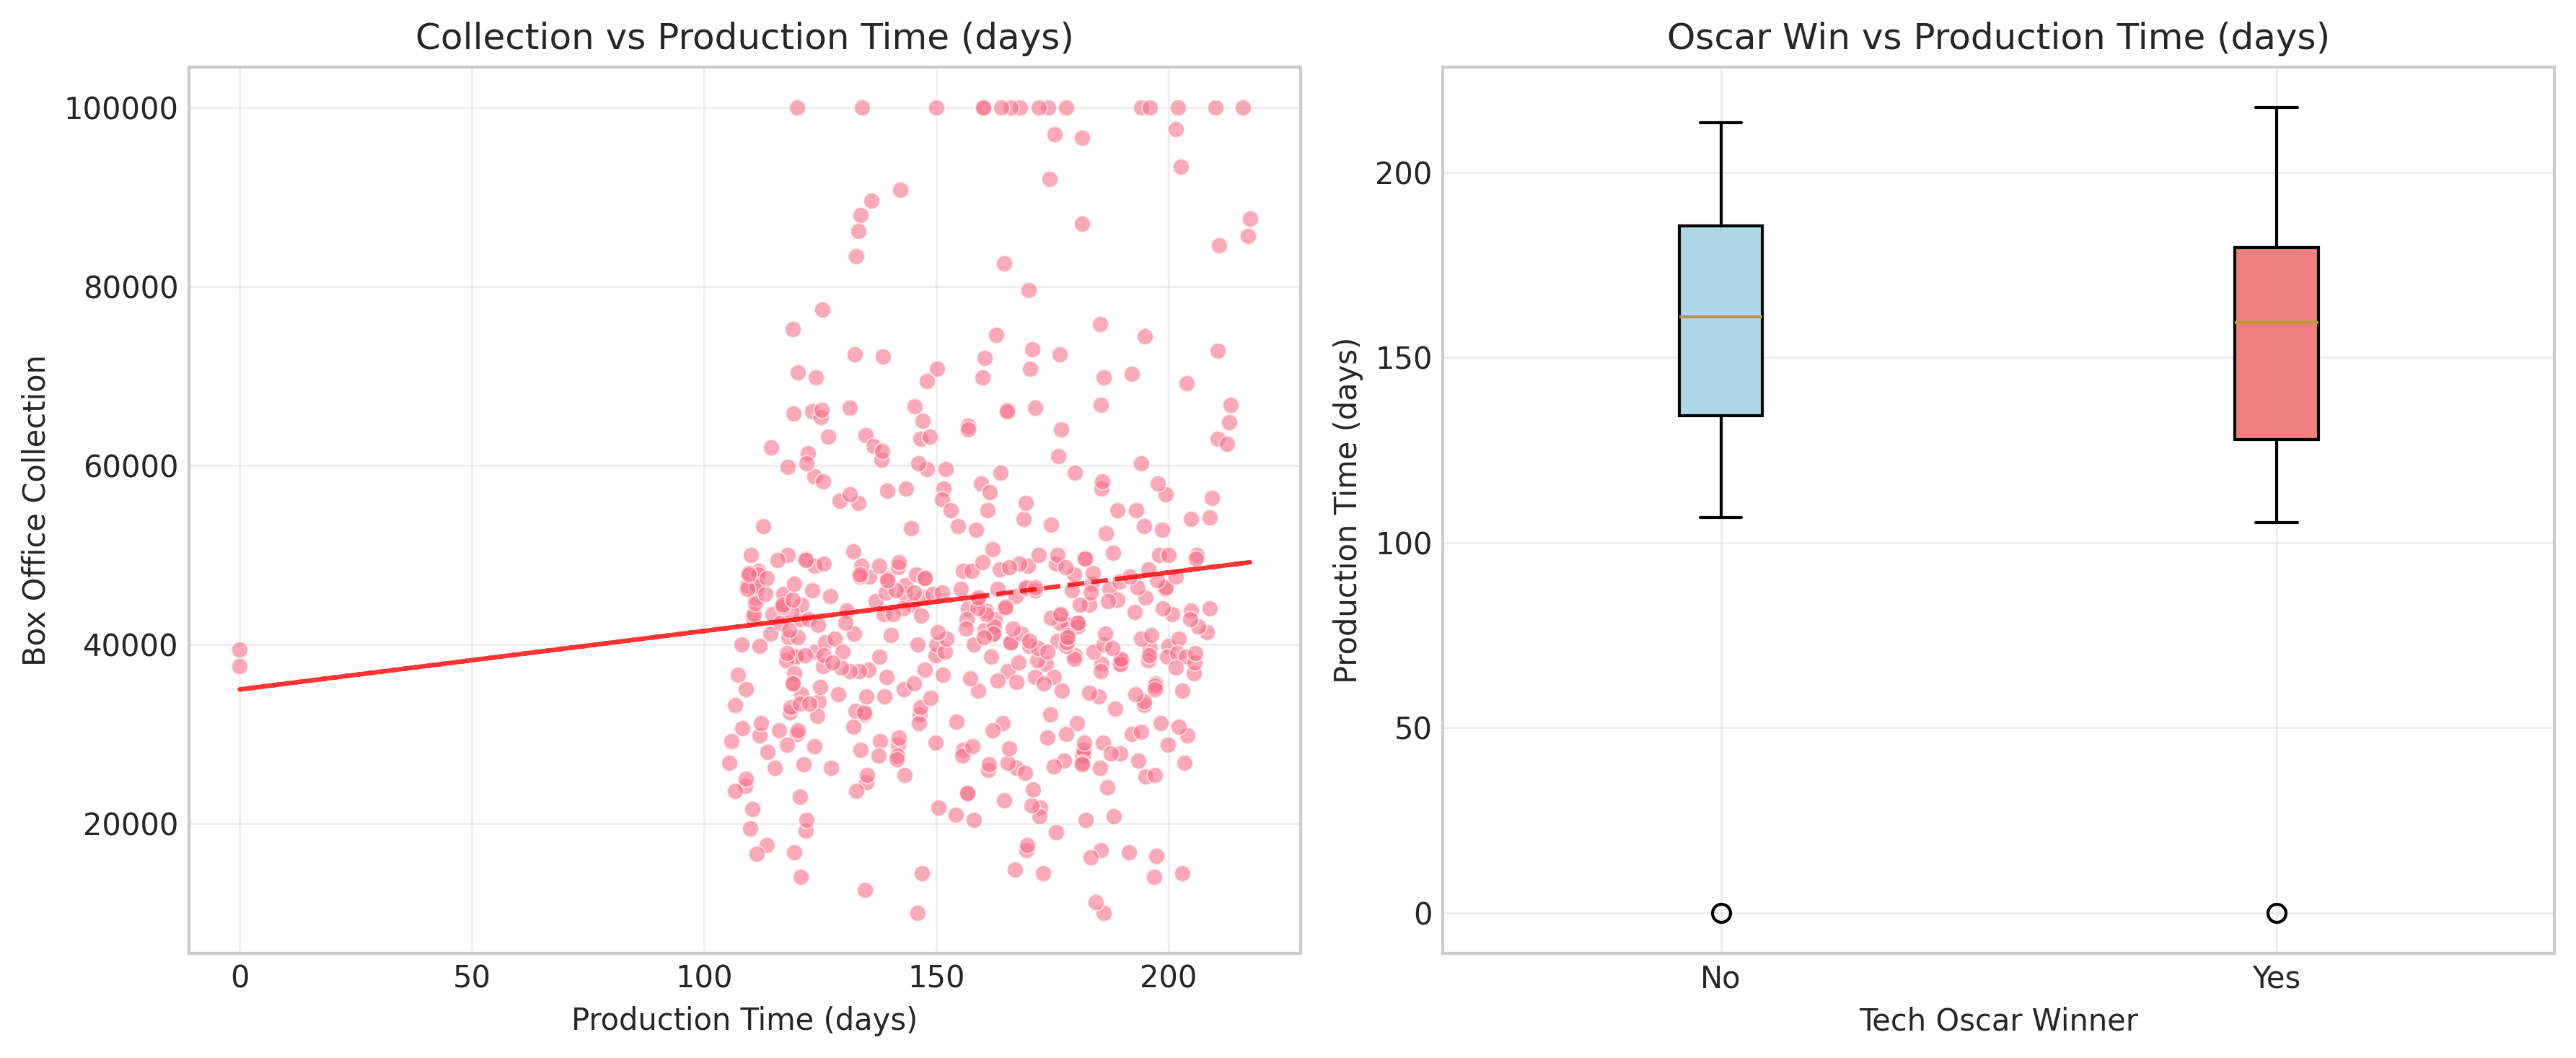
\includegraphics[width=0.9\textwidth]{../DatasetAnalysis/plots/Time_taken.png}
    \caption{Production time distribution}
\end{figure}
\begin{figure}
    \centering
    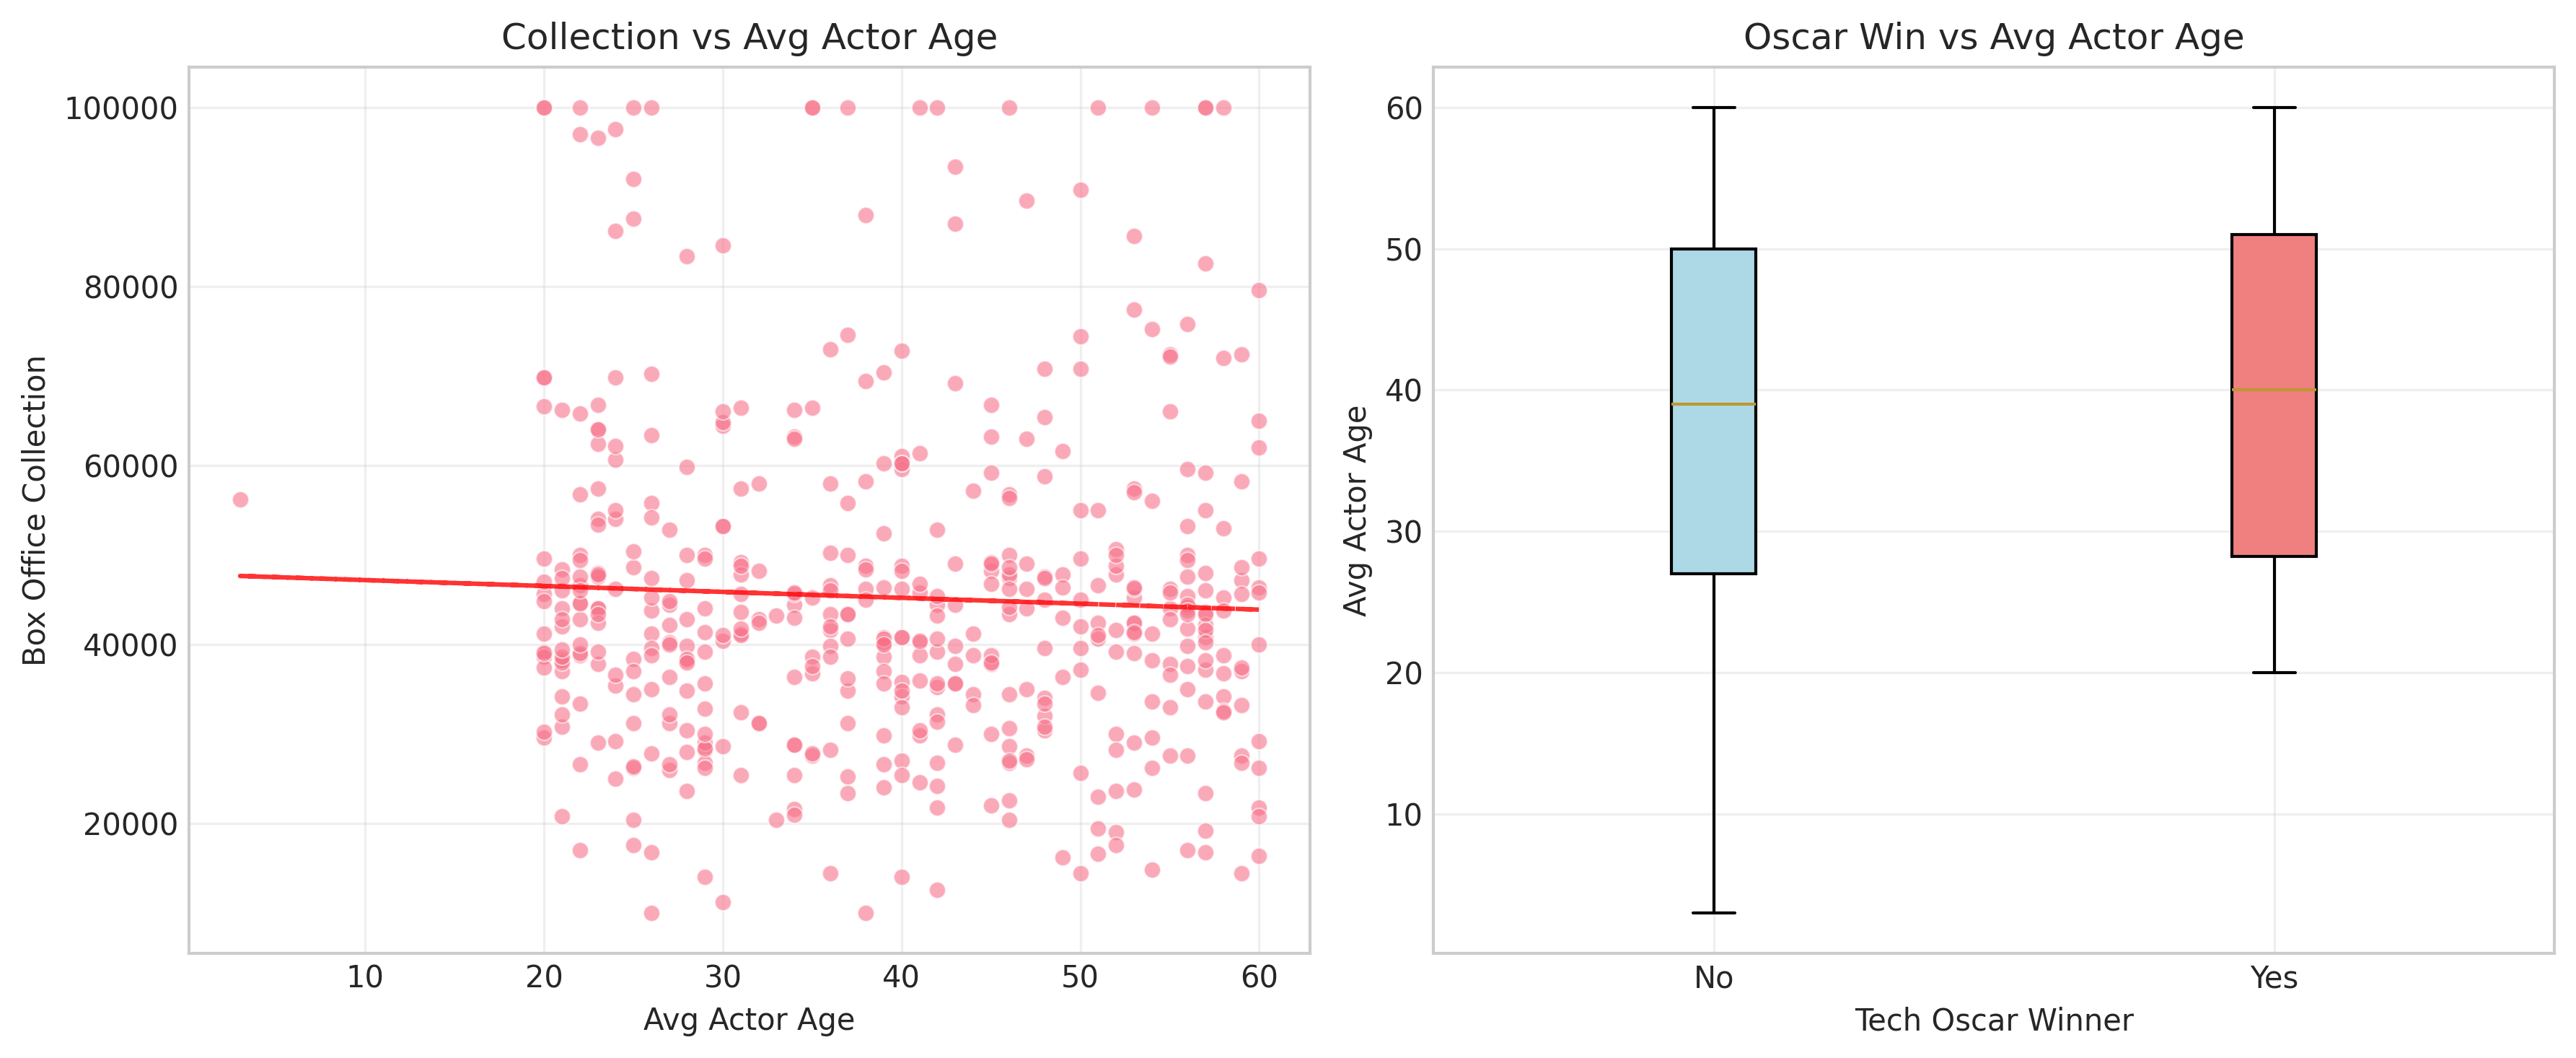
\includegraphics[width=0.9\textwidth]{../DatasetAnalysis/plots/Avg_age_actors.png}
    \caption{Average actor age distribution}
\end{figure}
\end{column}
\end{columns}
\end{frame}

\begin{frame}{Appendix: Feature Distributions - Social \& Distribution}
\begin{columns}
\begin{column}{0.5\textwidth}
\begin{figure}
    \centering
    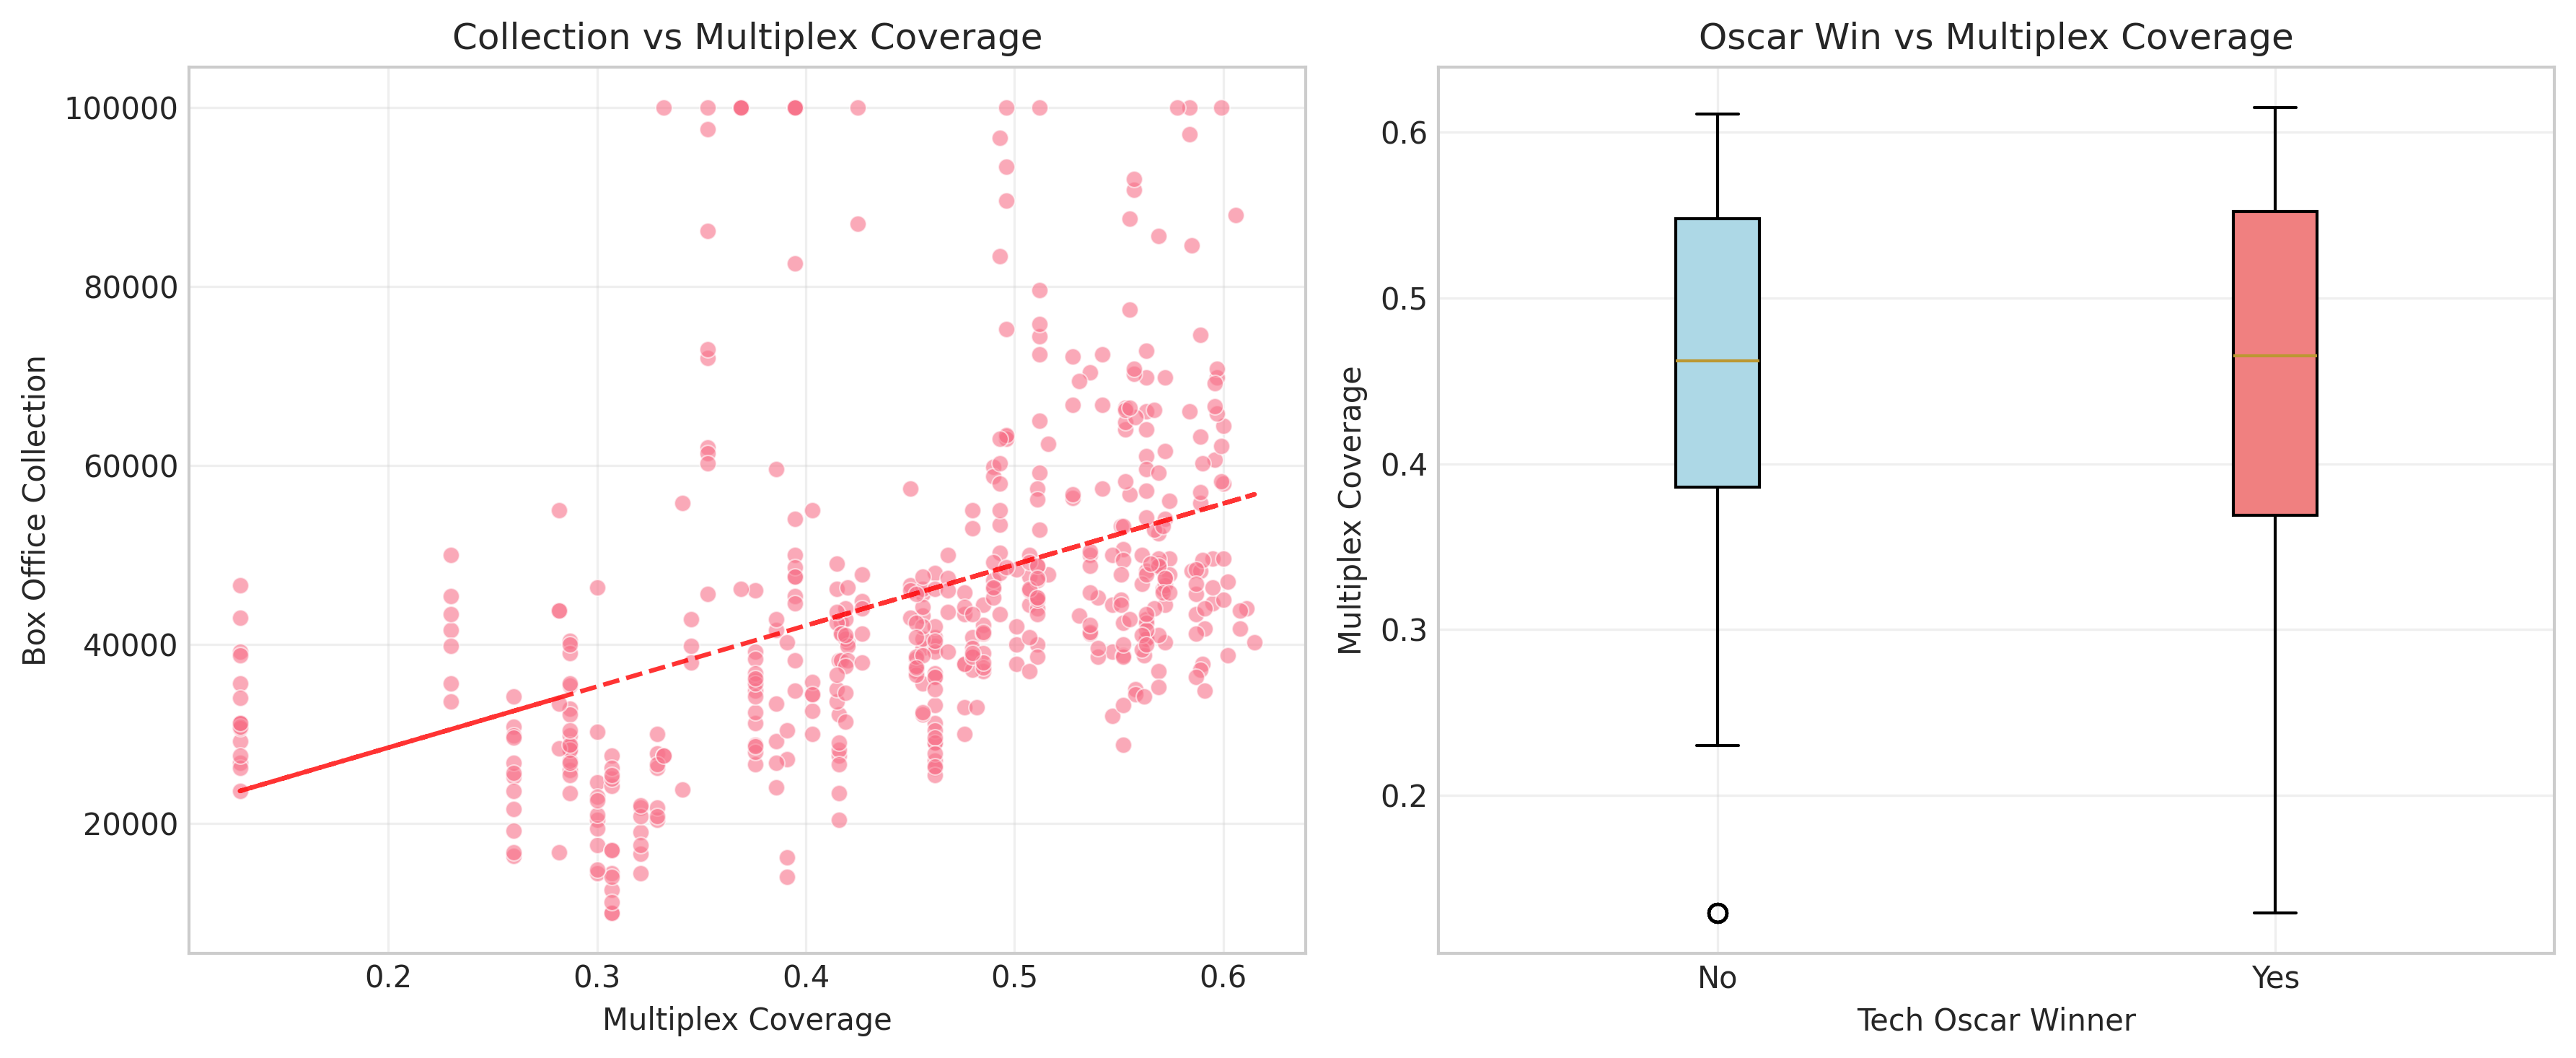
\includegraphics[width=0.9\textwidth]{../DatasetAnalysis/plots/Multiplex_coverage.png}
    \caption{Multiplex coverage distribution}
\end{figure}
\begin{figure}
    \centering
    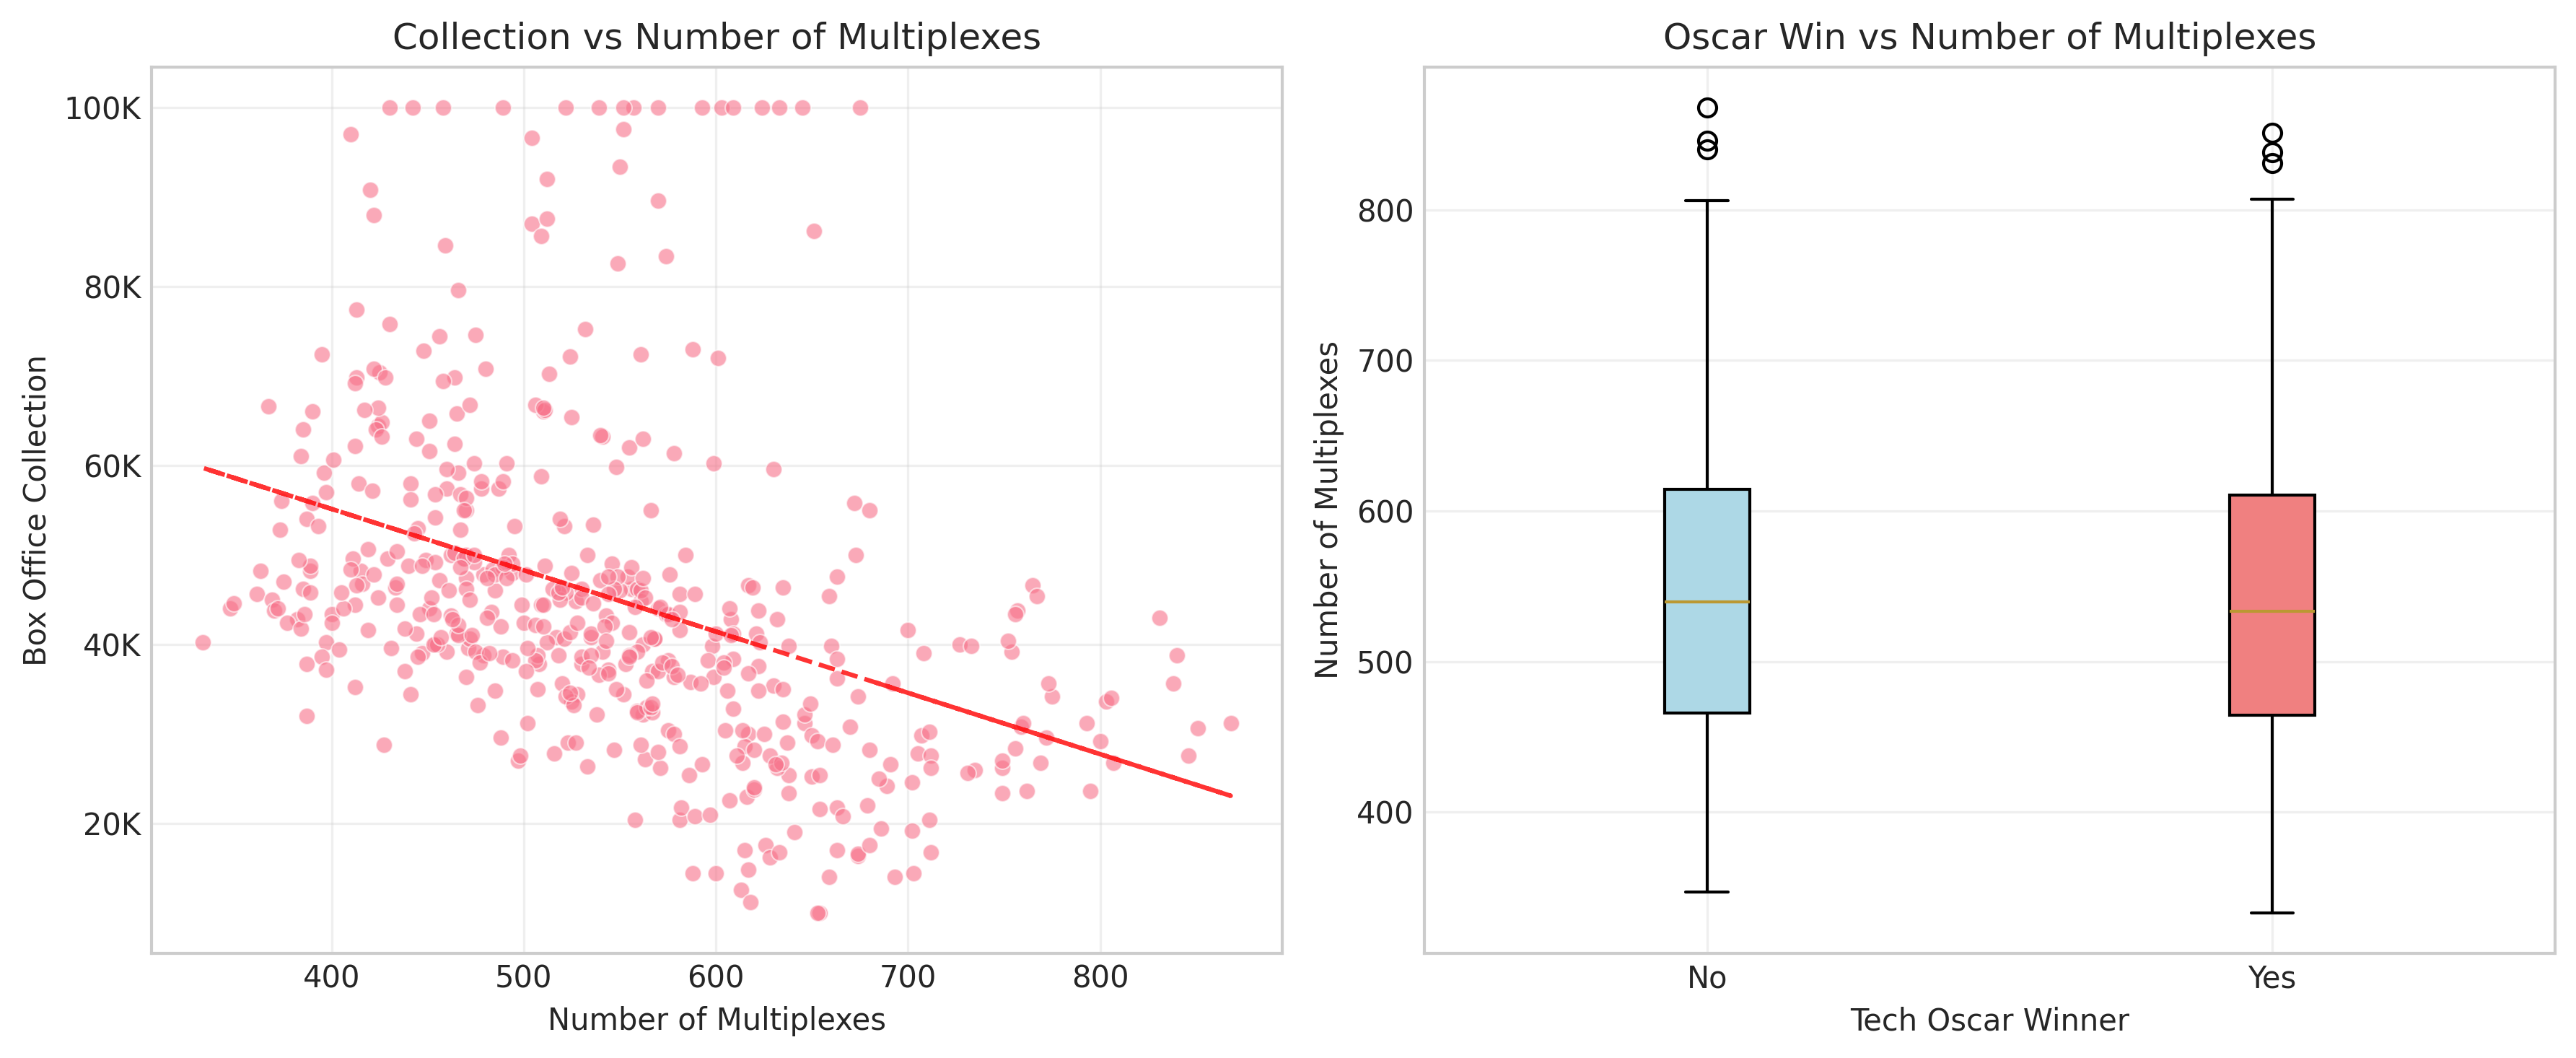
\includegraphics[width=0.9\textwidth]{../DatasetAnalysis/plots/Num_multiplex.png}
    \caption{Number of multiplexes distribution}
\end{figure}
\end{column}
\begin{column}{0.5\textwidth}
\begin{figure}
    \centering
    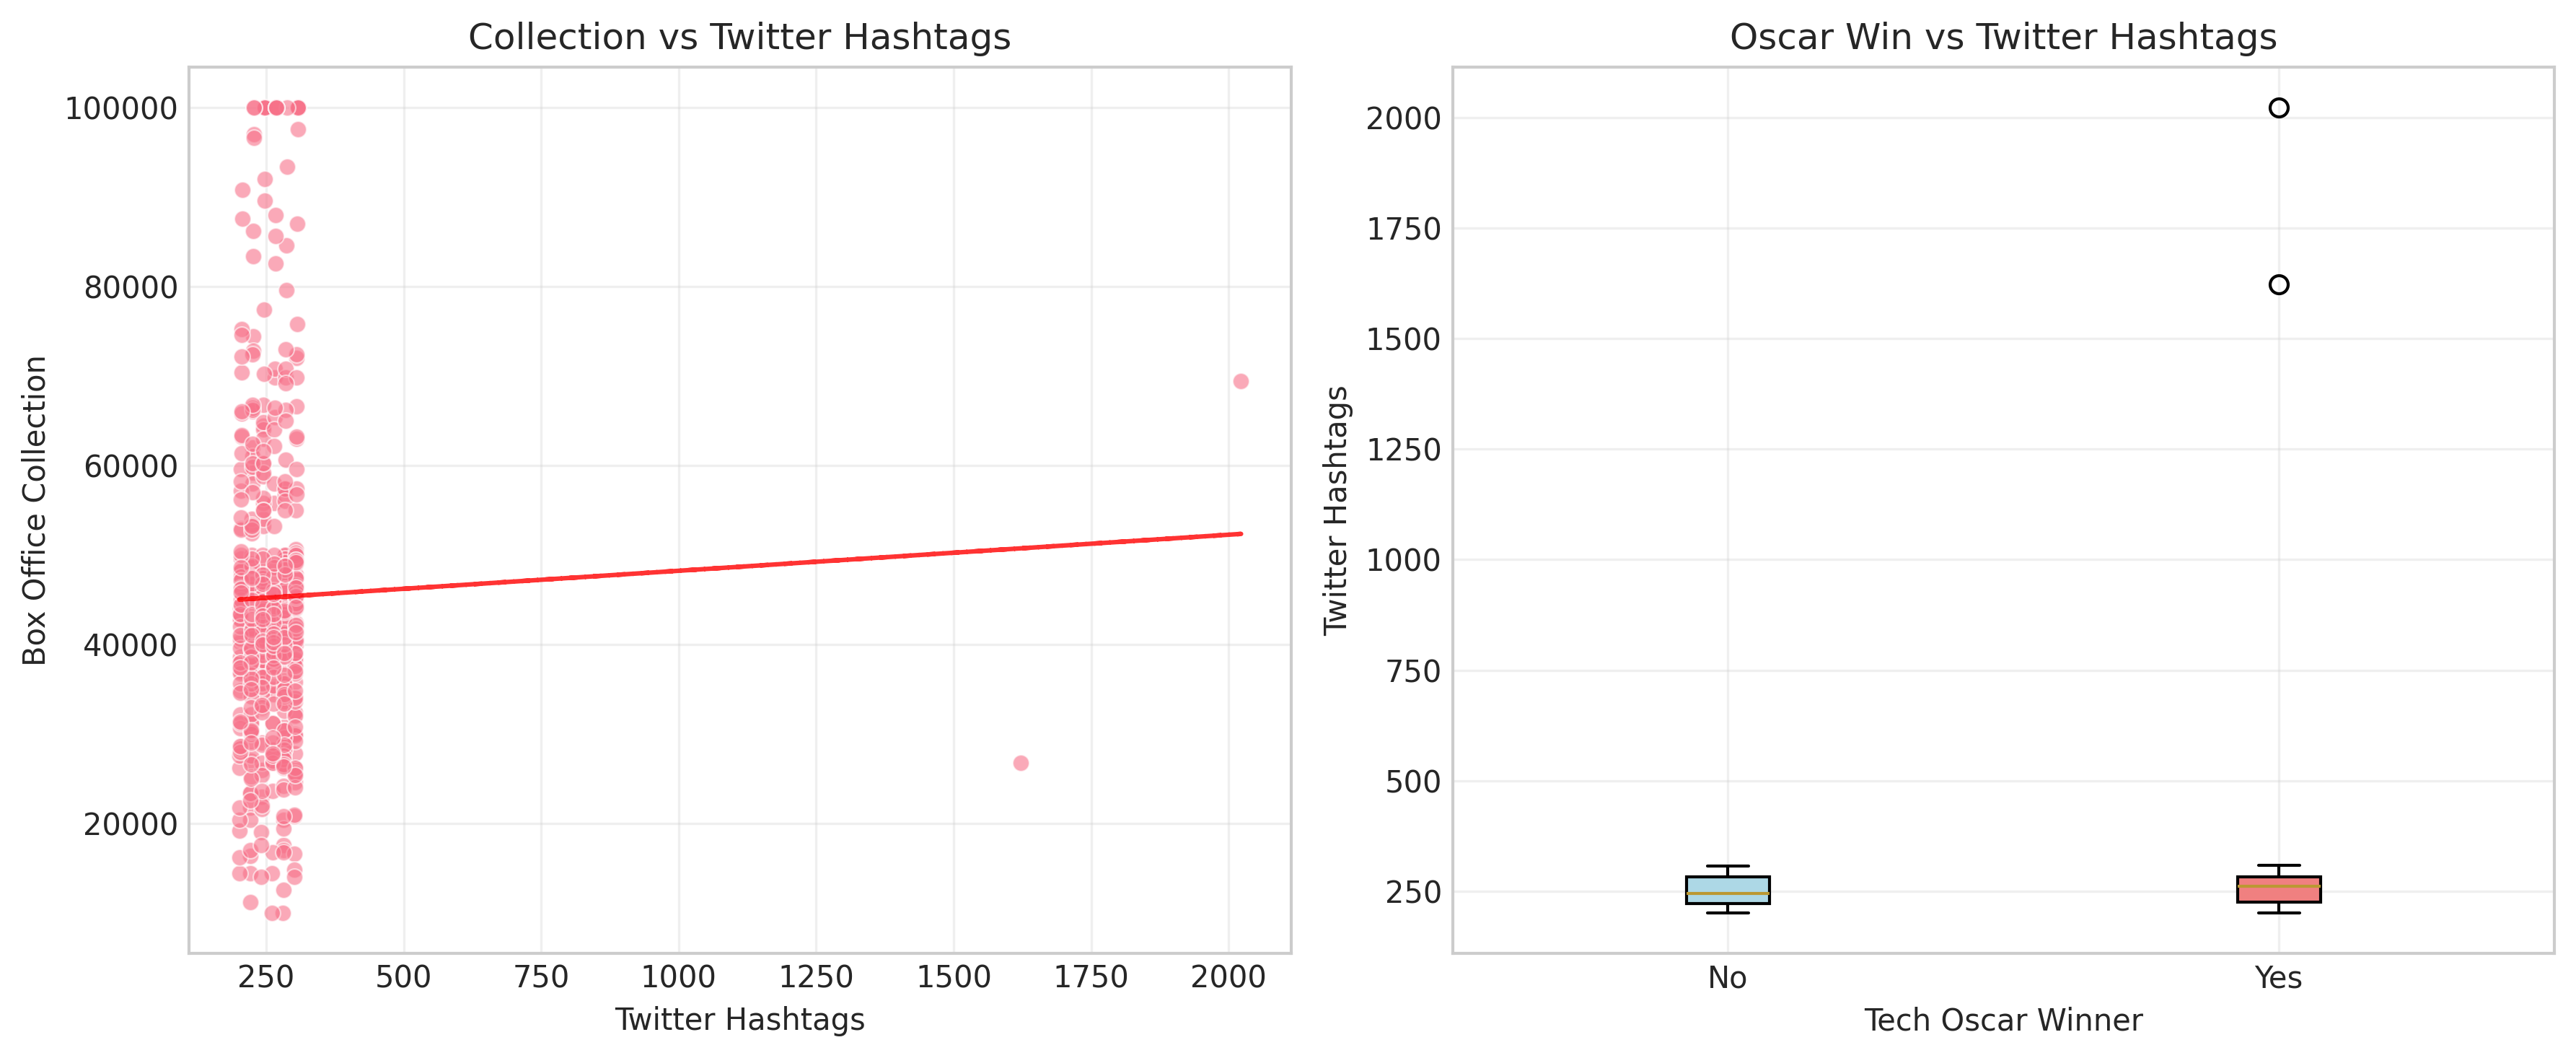
\includegraphics[width=0.9\textwidth]{../DatasetAnalysis/plots/Twitter_hastags.png}
    \caption{Twitter hashtags distribution}
\end{figure}
\begin{figure}
    \centering
    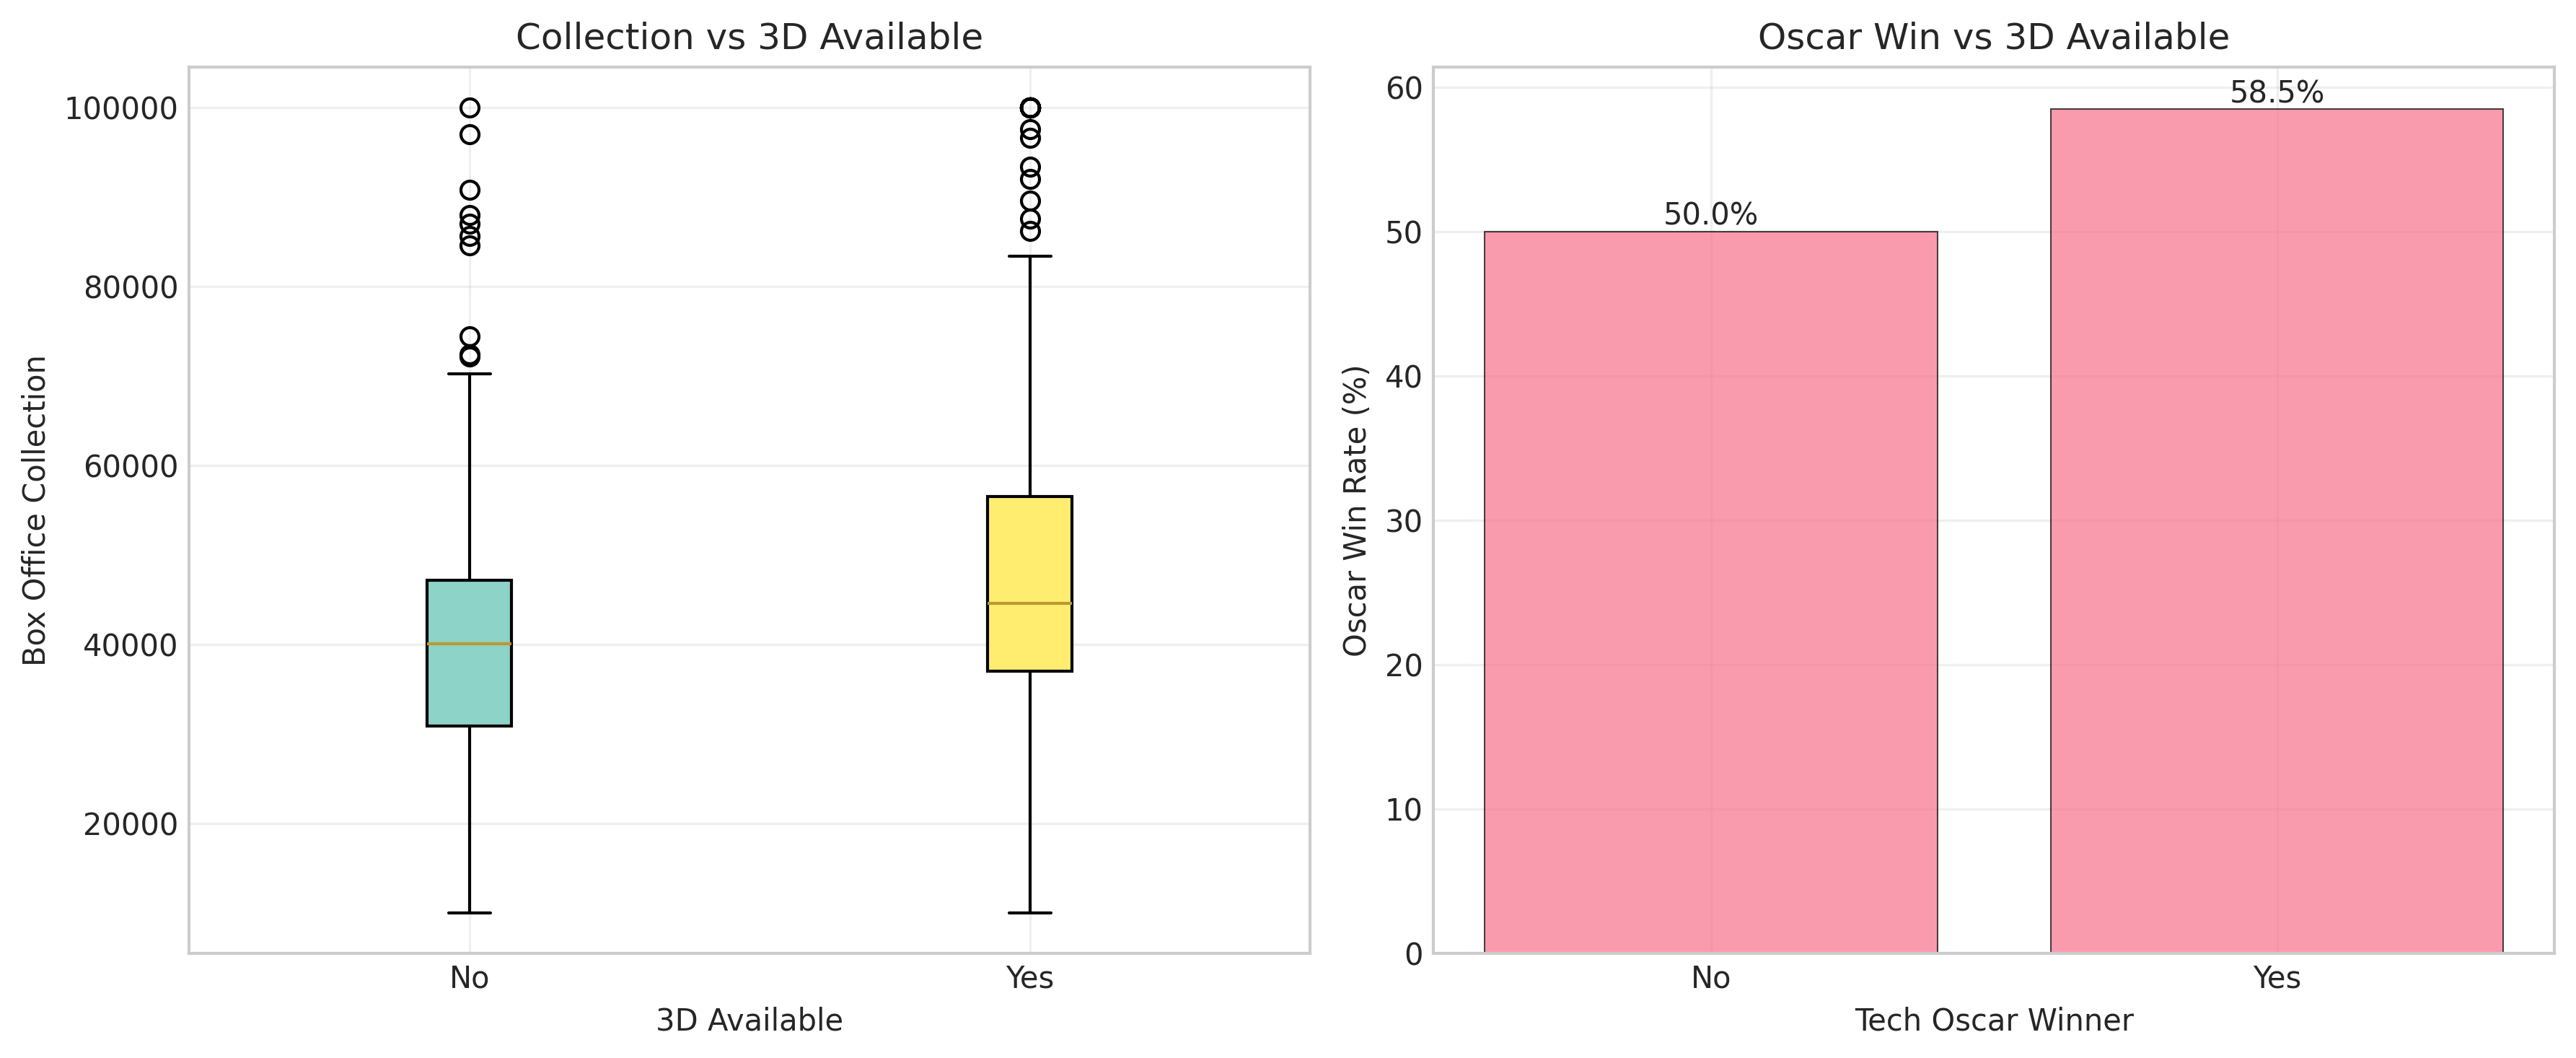
\includegraphics[width=0.9\textwidth]{../DatasetAnalysis/plots/3D_available.png}
    \caption{3D availability distribution}
\end{figure}
\end{column}
\end{columns}
\end{frame}

\begin{frame}{Appendix: Categorical Feature - Genre Distribution}
\begin{figure}
    \centering
    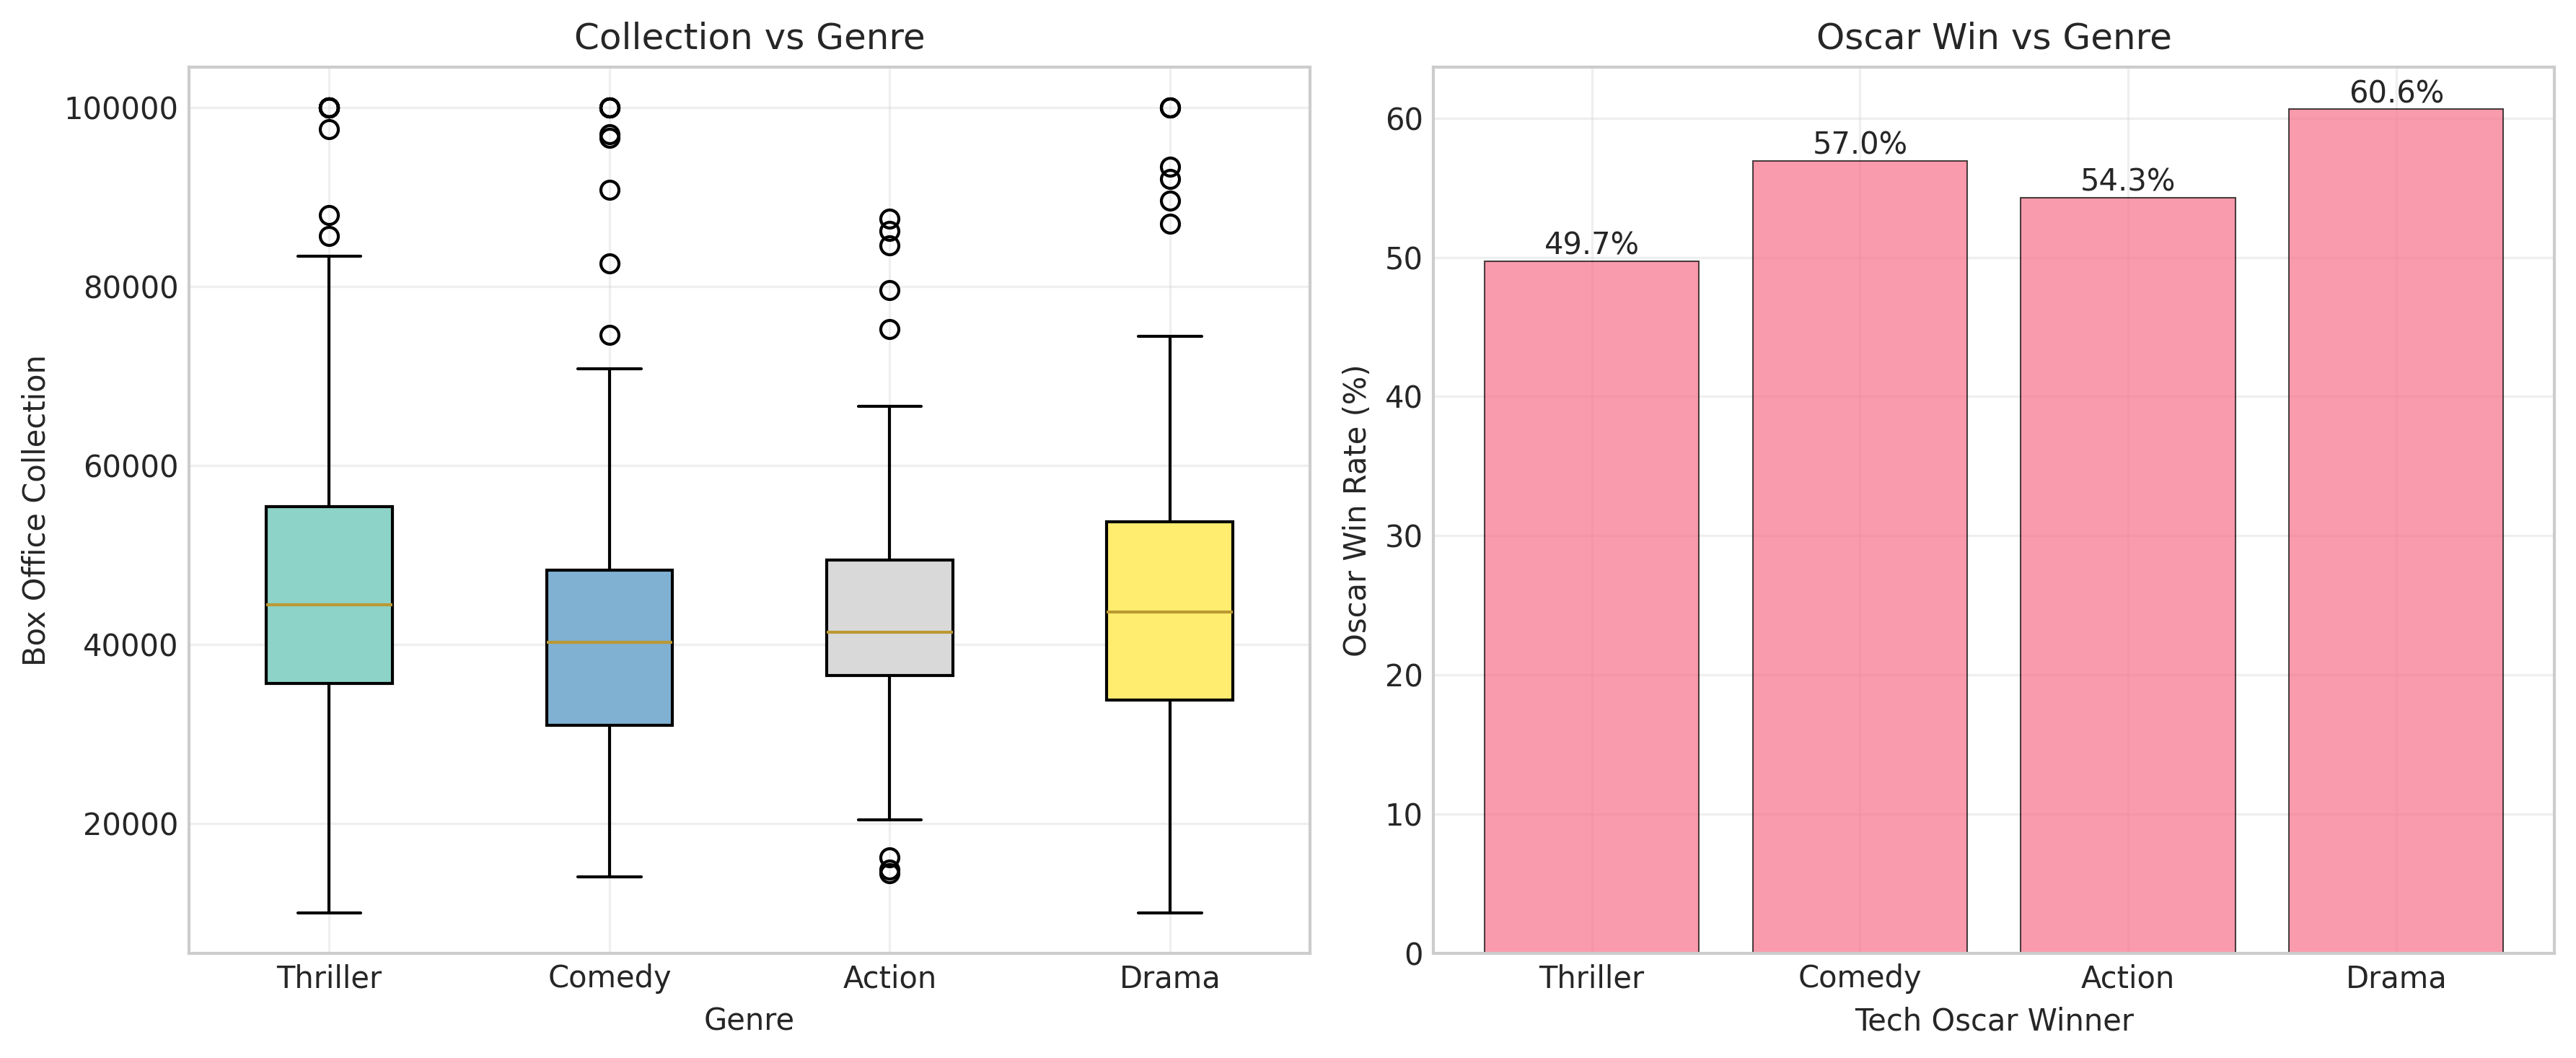
\includegraphics[width=0.8\textwidth]{../DatasetAnalysis/plots/Genre.png}
    \caption{Genre distribution across the dataset}
\end{figure}
\begin{center}
\textbf{Note}: Genre was one-hot encoded for model training, providing important categorical information for classification.
\end{center}
\end{frame}

\begin{frame}{Appendix: Target Variable Analysis}
\begin{columns}
\begin{column}{0.6\textwidth}
\begin{figure}
    \centering
    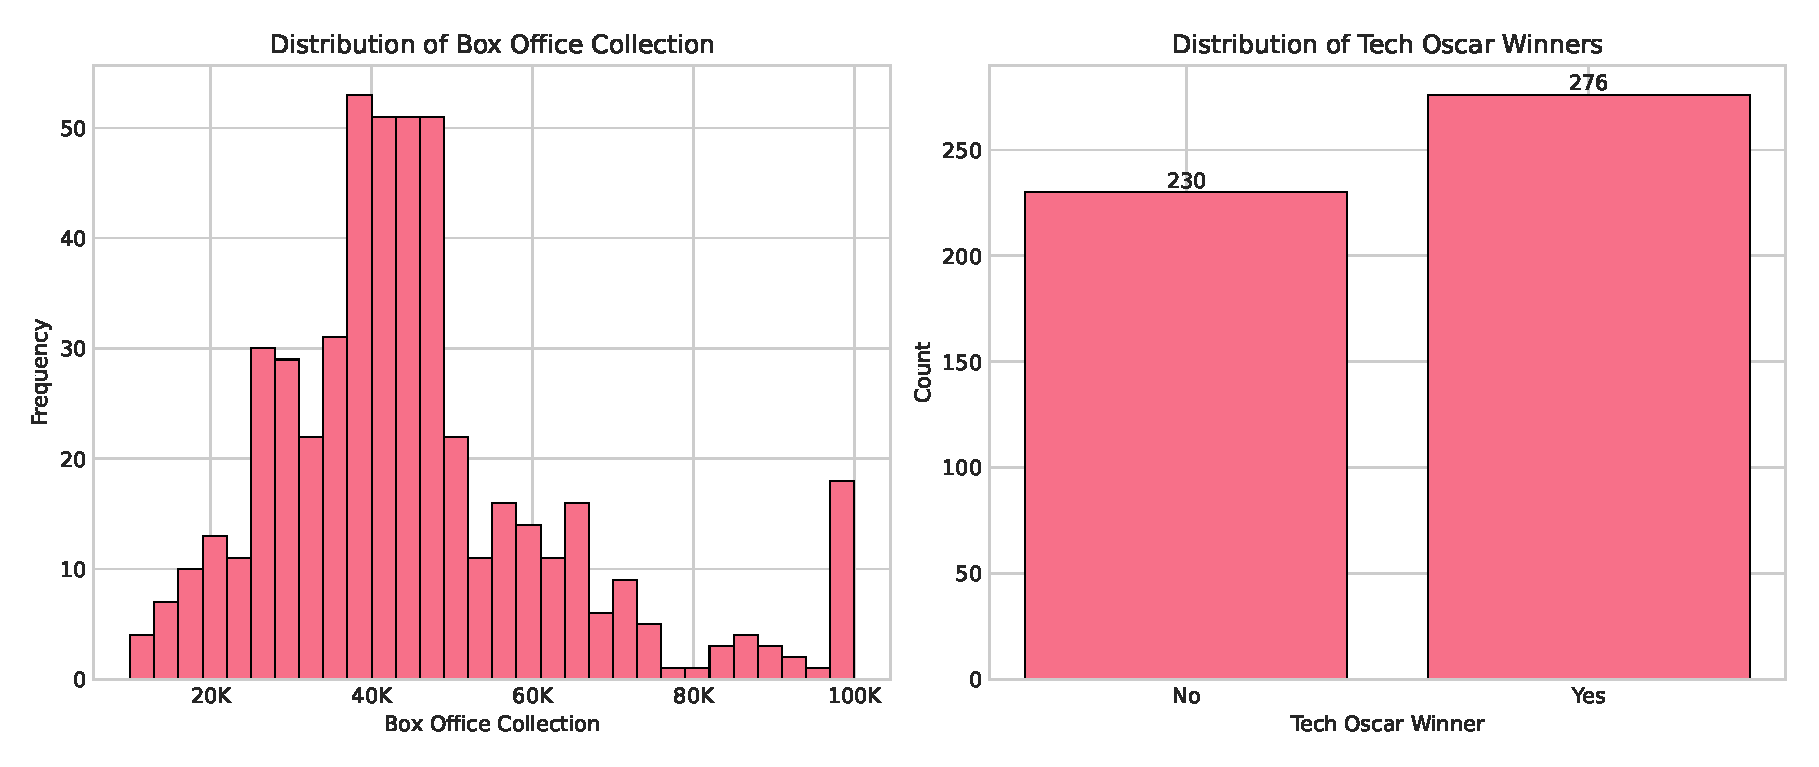
\includegraphics[width=\textwidth]{../DatasetAnalysis/target_histograms.eps}
    \caption{Target variable distributions (Start\_Tech\_Oscar \& Collection)}
\end{figure}
\end{column}
\begin{column}{0.4\textwidth}
\begin{block}{Target Variables}
\begin{itemize}
\item \textbf{Start\_Tech\_Oscar}: Technical Oscar nomination
\item \textbf{Collection}: Box office collection success
\item Both are binary classification targets
\item Balanced distribution enables effective learning
\end{itemize}
\end{block}
\end{column}
\end{columns}
\end{frame}

\begin{frame}{Appendix: Model Performance Across All Preprocessing}
\begin{table}
\centering
\tiny
\begin{tabular}{lcccccc}
\toprule
\textbf{Model} & \textbf{Unclean} & \textbf{Robust} & \textbf{Winsorize} & \textbf{Quantile} & \textbf{Isolation Forest} & \textbf{Best} \\
\midrule
KNN\_Cosine & 0.7412 & 0.7523 & 0.7389 & 0.7214 & \textbf{0.8734} & \textbf{IF} \\
MLP\_1Layer & 0.6987 & 0.7123 & 0.7056 & 0.6945 & \textbf{0.8524} & \textbf{IF} \\
RandomForest & 0.6821 & 0.6954 & 0.6889 & 0.6712 & \textbf{0.8480} & \textbf{IF} \\
LDA & 0.6543 & 0.6678 & 0.6591 & 0.6456 & \textbf{0.7059} & \textbf{IF} \\
RbfSVM & 0.6321 & 0.6489 & 0.6398 & 0.6214 & \textbf{0.7208} & \textbf{IF} \\
LinearSVM & 0.5987 & 0.6123 & 0.6045 & 0.5891 & 0.6543 & IF \\
DecisionTree & 0.5678 & 0.5812 & 0.5734 & 0.5589 & 0.6234 & IF \\
GaussianNB & 0.5234 & 0.5389 & 0.5291 & 0.5123 & 0.5891 & IF \\
\bottomrule
\end{tabular}
\caption{F1-scores across preprocessing methods (with feature dropping)}
\end{table}

\begin{center}
\textbf{Key Insight}: Isolation Forest preprocessing consistently outperforms other methods across all model types
\end{center}
\end{frame}

\begin{frame}{Appendix: Feature Importance Analysis}
\begin{columns}
\begin{column}{0.6\textwidth}
\begin{figure}
    \centering
    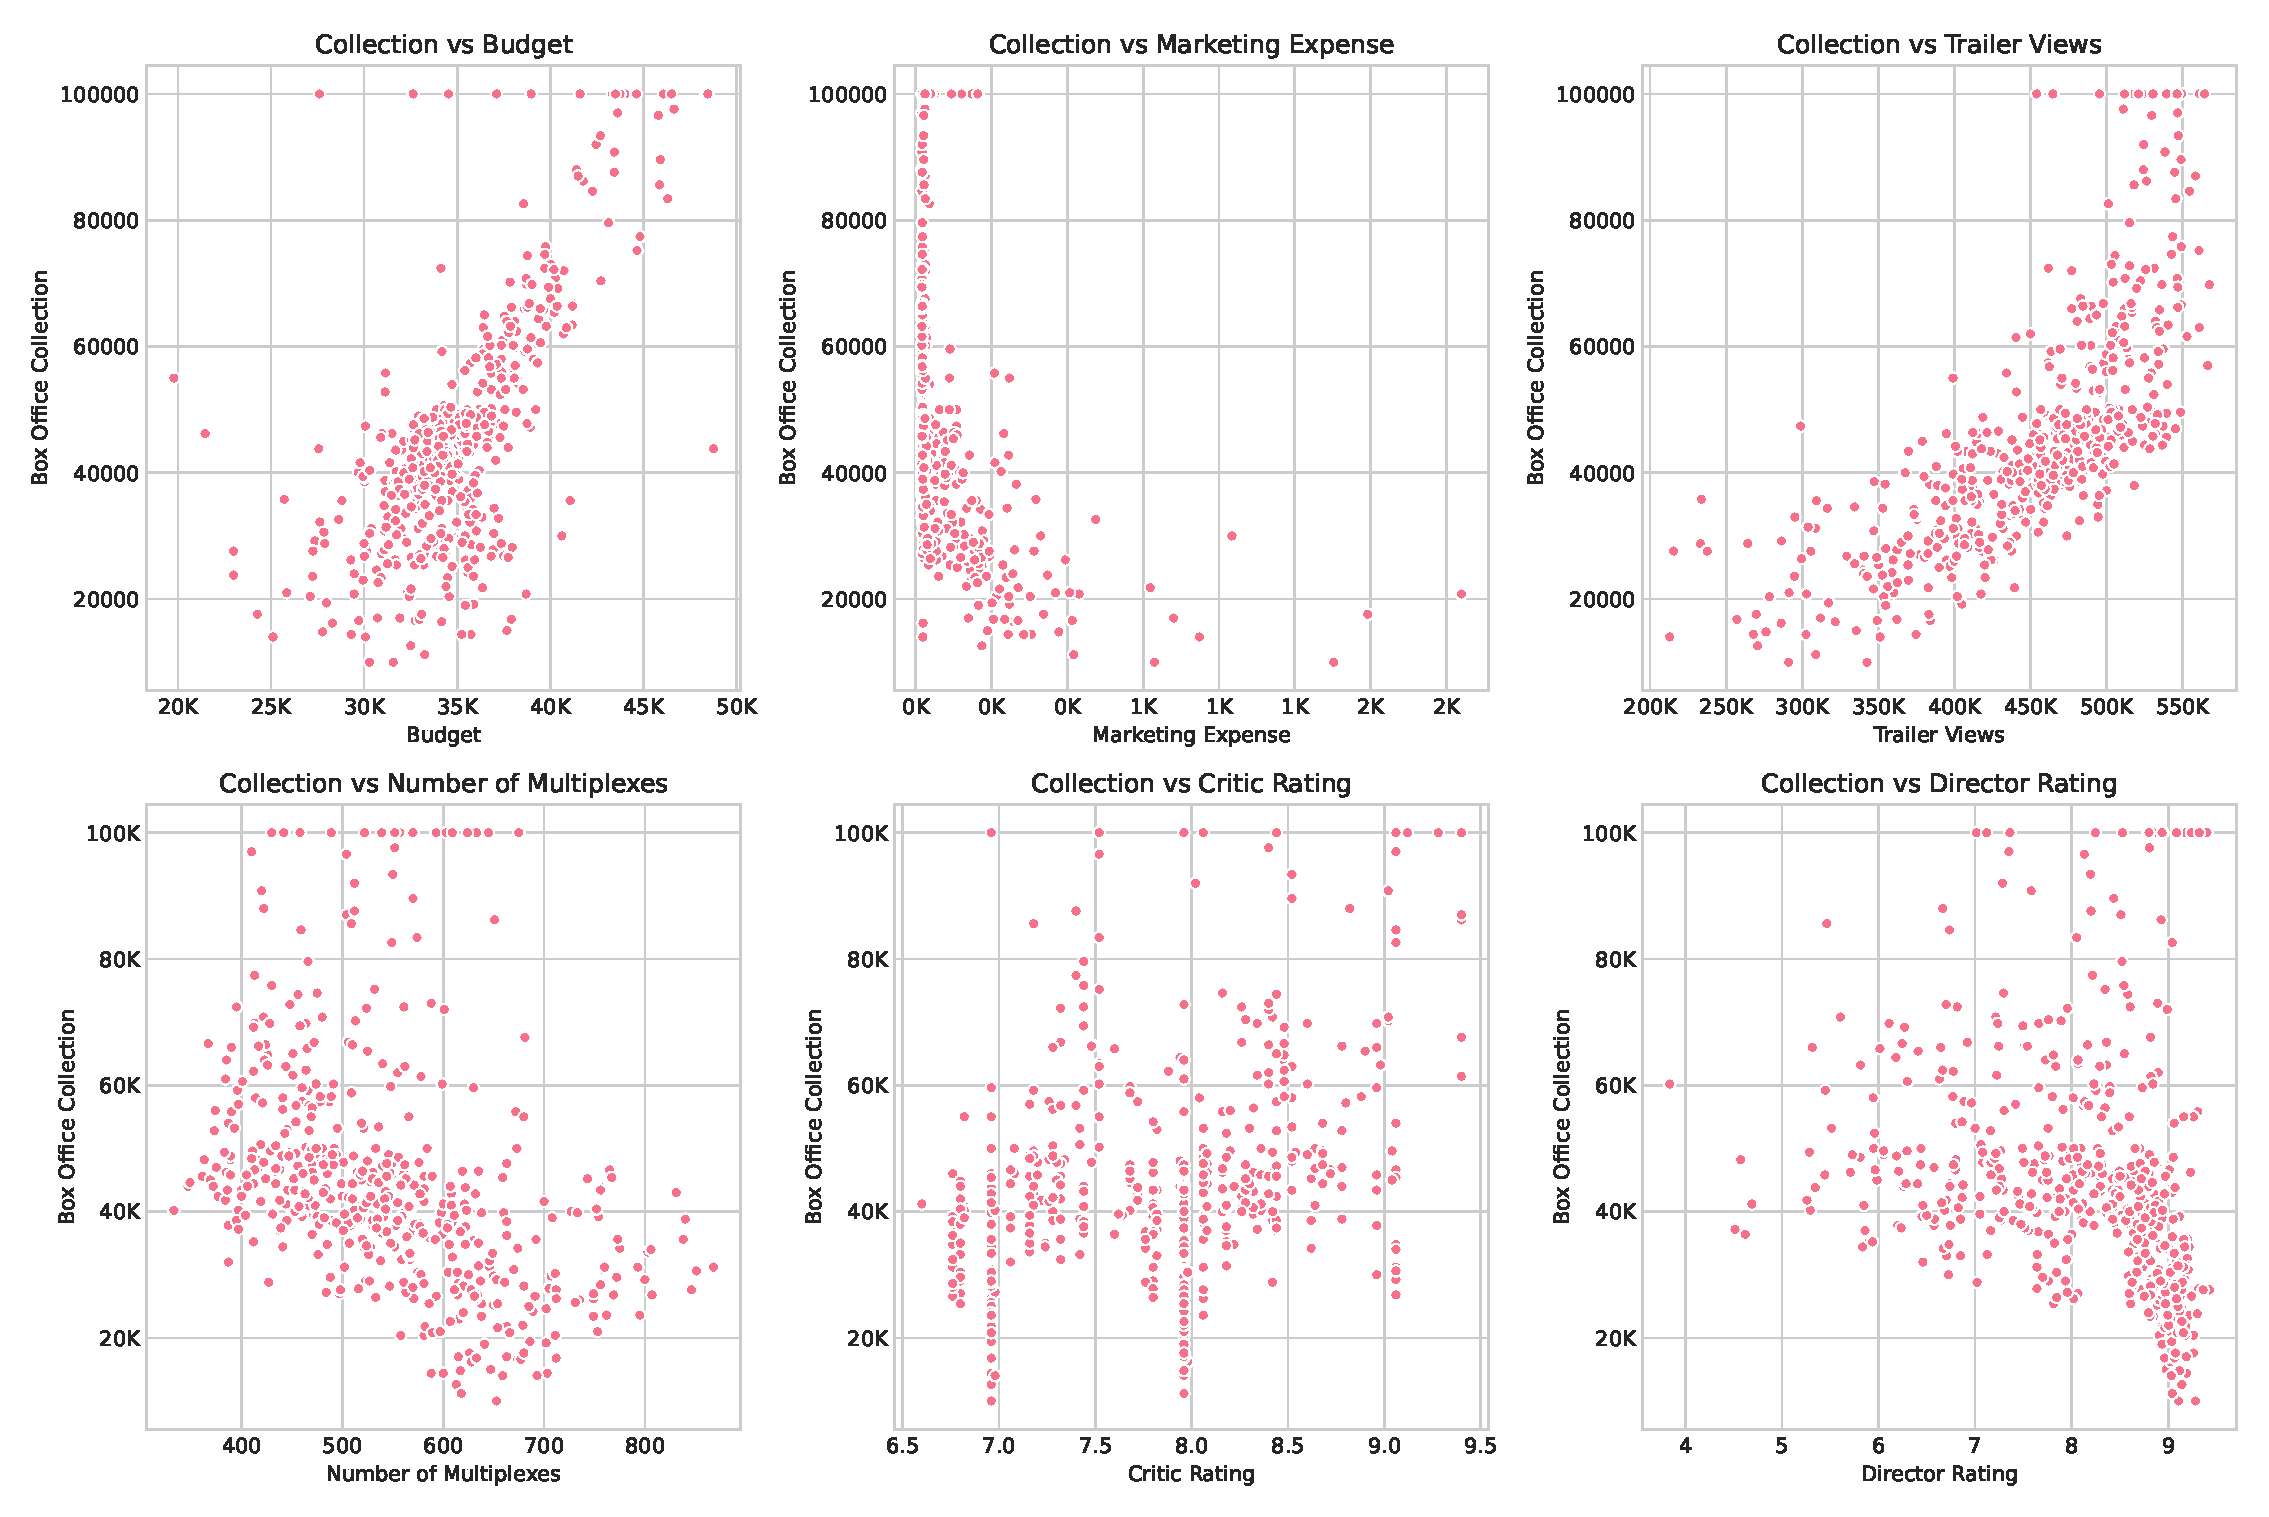
\includegraphics[width=\textwidth]{../DatasetAnalysis/collection_scatters.eps}
    \caption{Feature importance for collection prediction}
\end{figure}
\end{column}
\begin{column}{0.4\textwidth}
\begin{block}{Top Predictive Features}
\begin{itemize}
\item \textbf{Critic Rating}: Strongest predictor
\item \textbf{Budget}: Significant impact
\item \textbf{Trailer Views}: Marketing impact
\item \textbf{Director Rating}: Creative influence
\item \textbf{Production Expense}: Quality signal
\end{itemize}
\end{block}
\end{column}
\end{columns}
\end{frame}

\begin{frame}{Appendix: Advanced Feature Analysis}
\begin{columns}
\begin{column}{0.5\textwidth}
\begin{figure}
    \centering
    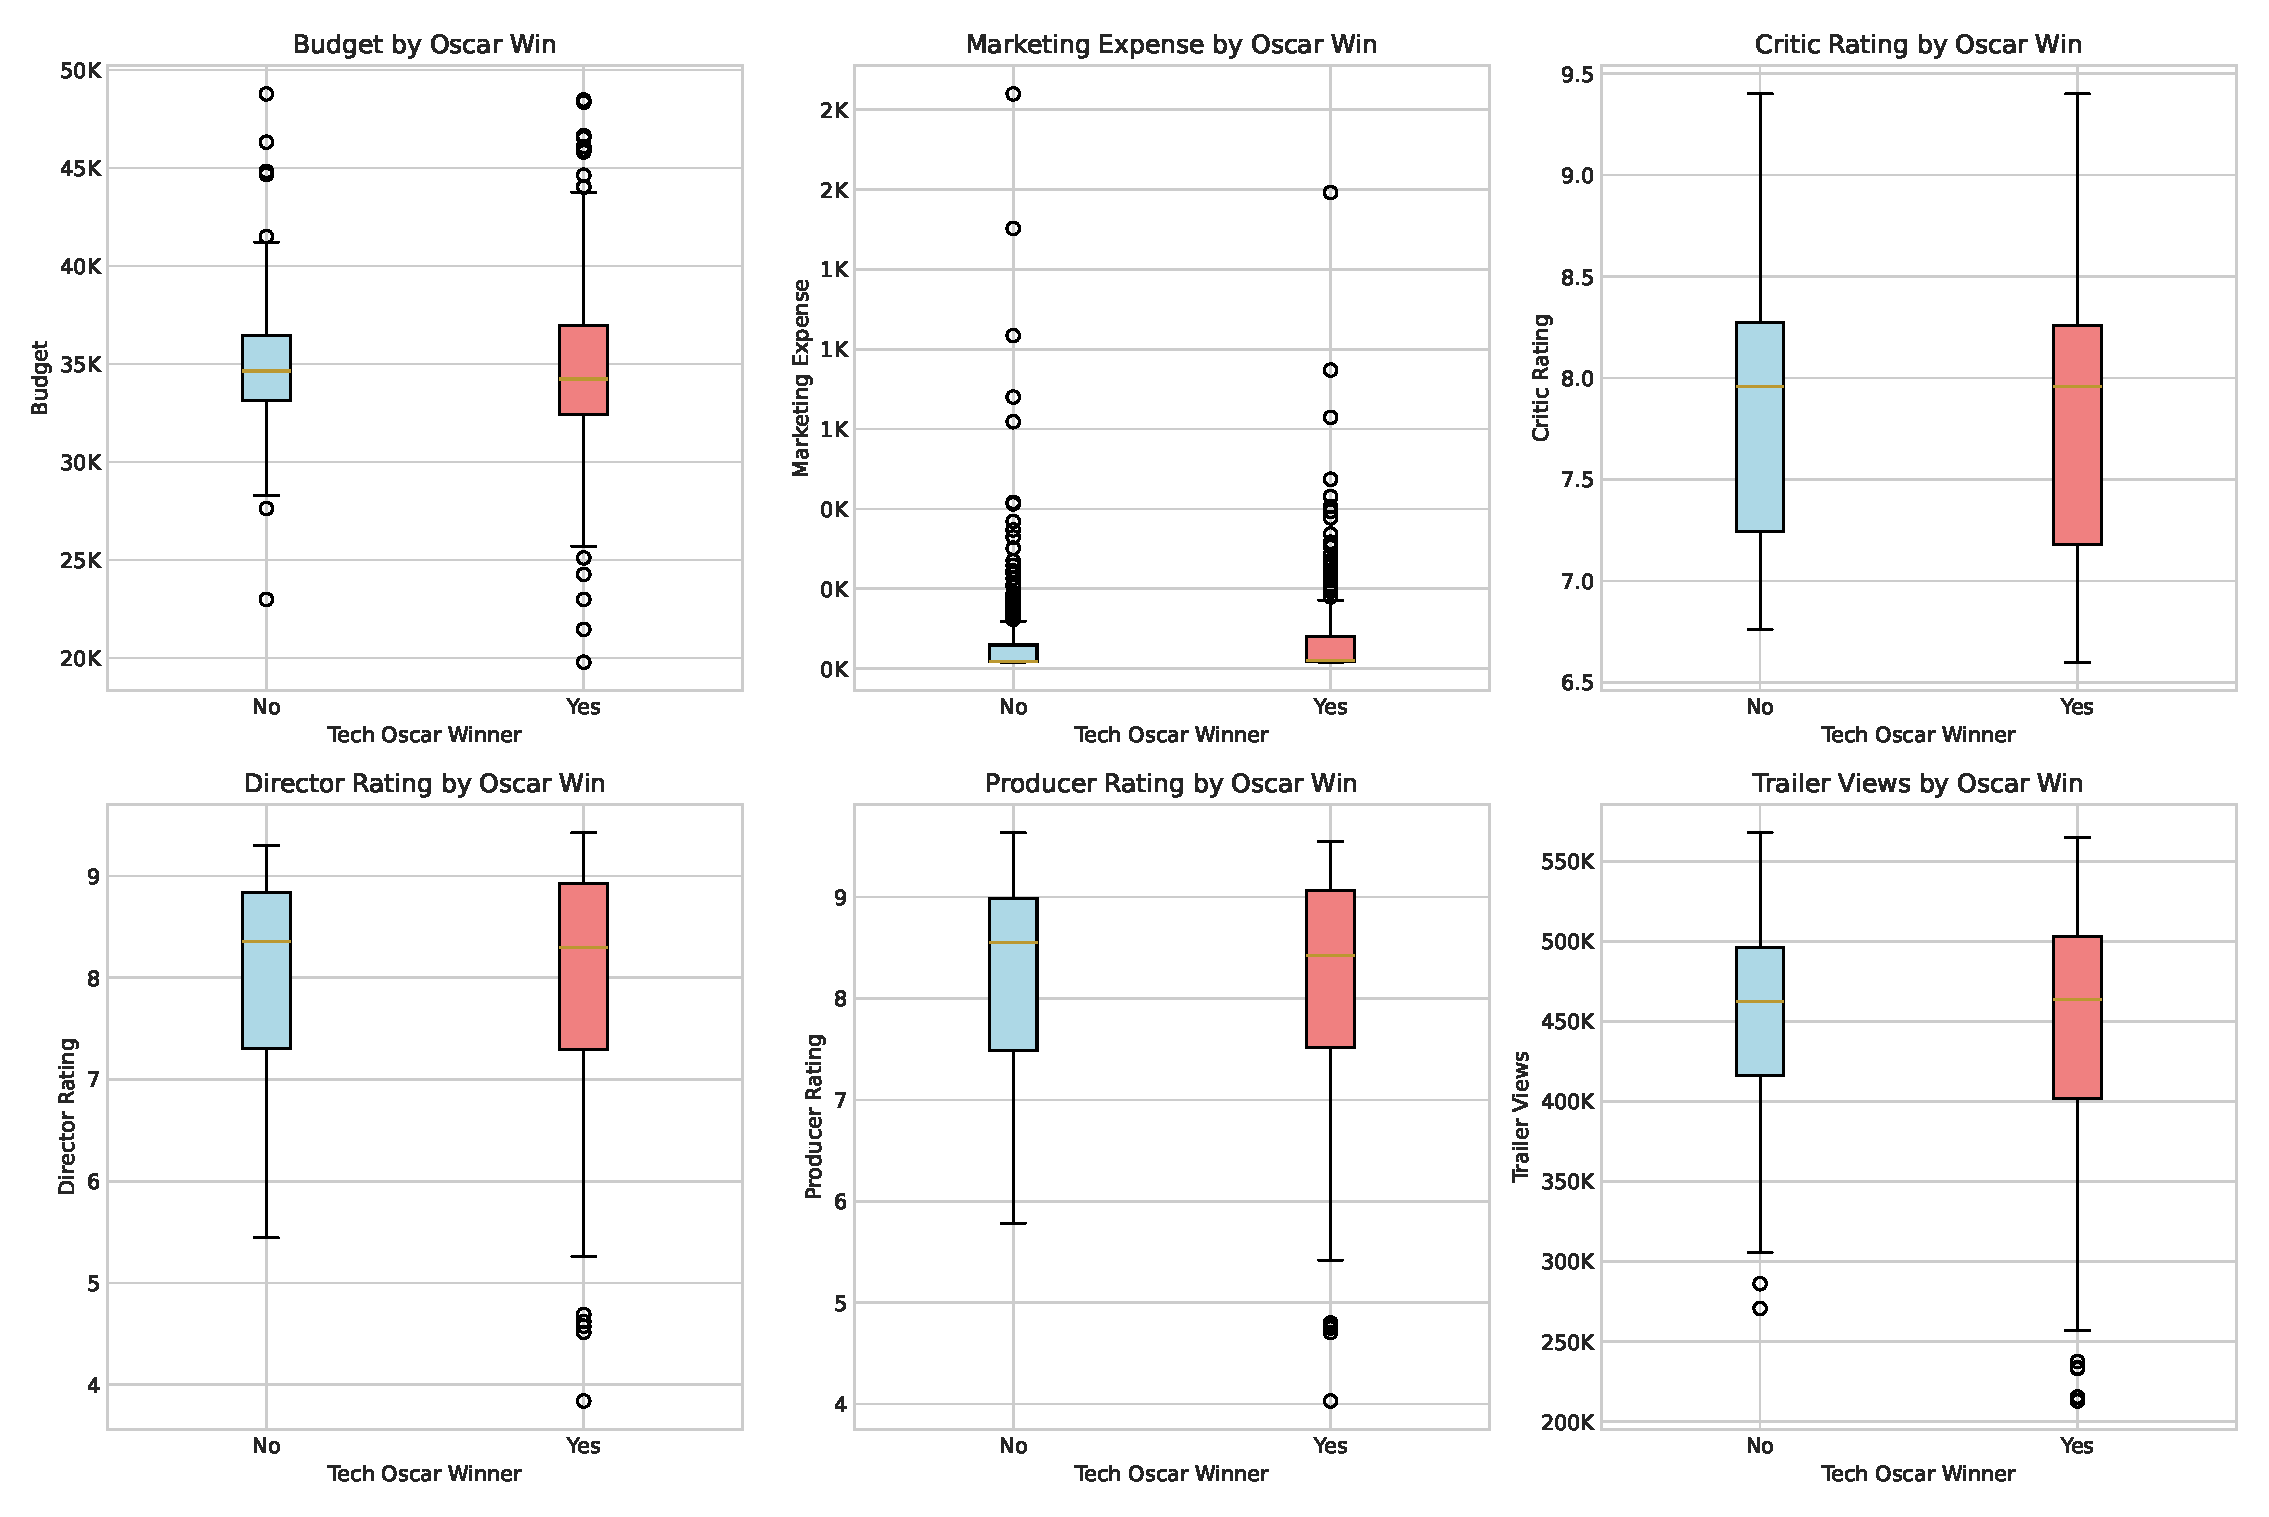
\includegraphics[width=0.9\textwidth]{../DatasetAnalysis/oscar_boxplots.eps}
    \caption{Oscar-related feature boxplots}
\end{figure}
\begin{figure}
    \centering
    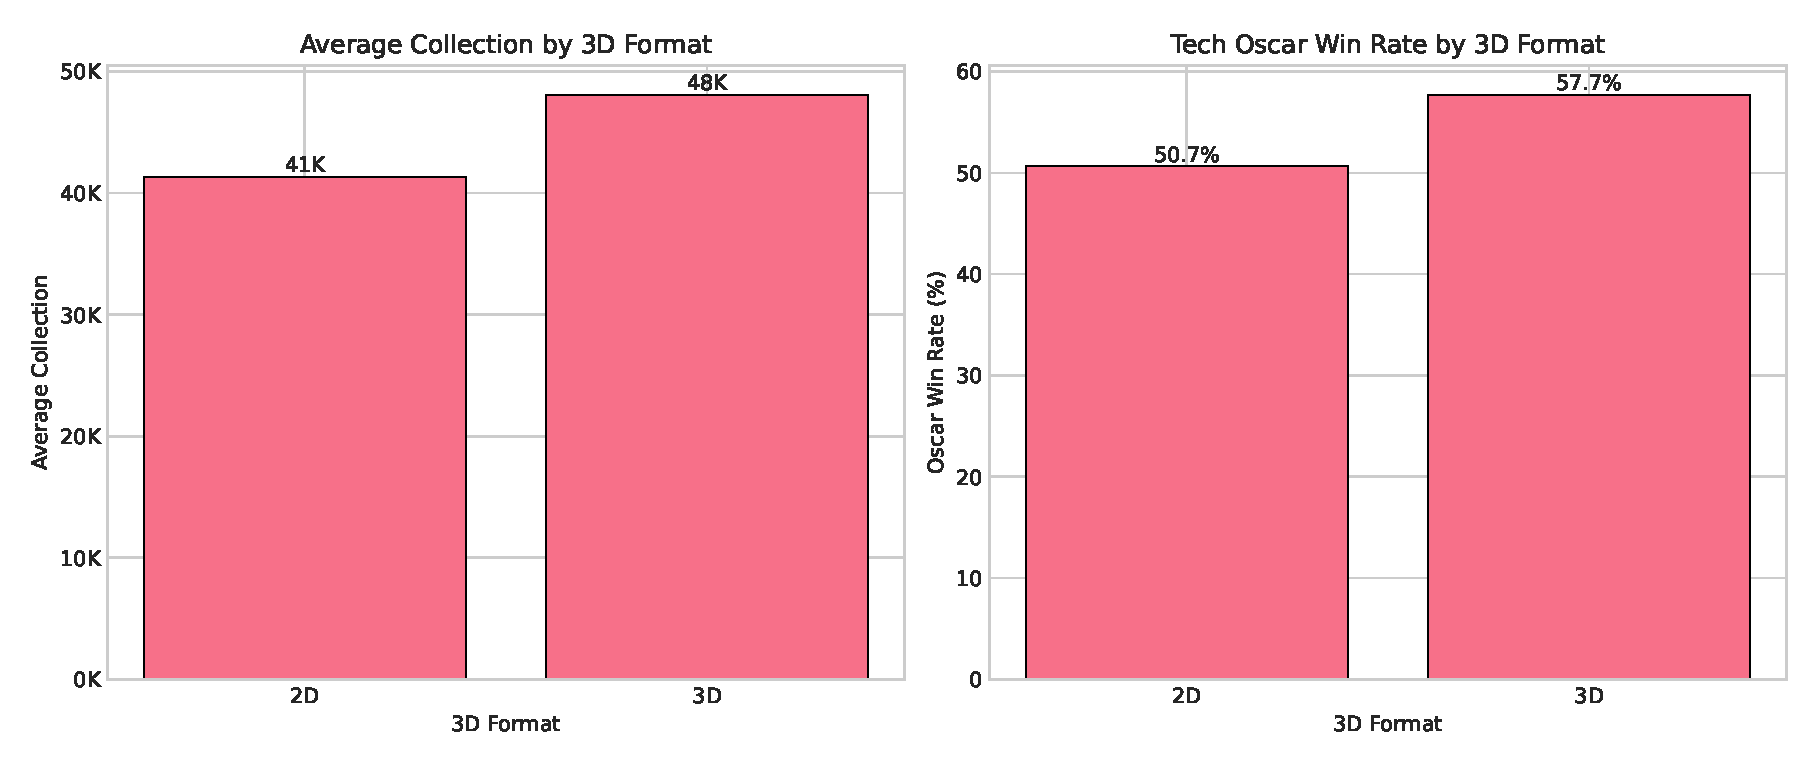
\includegraphics[width=0.9\textwidth]{../DatasetAnalysis/threed_analysis.eps}
    \caption{3D availability analysis}
\end{figure}
\end{column}
\begin{column}{0.5\textwidth}
\begin{figure}
    \centering
    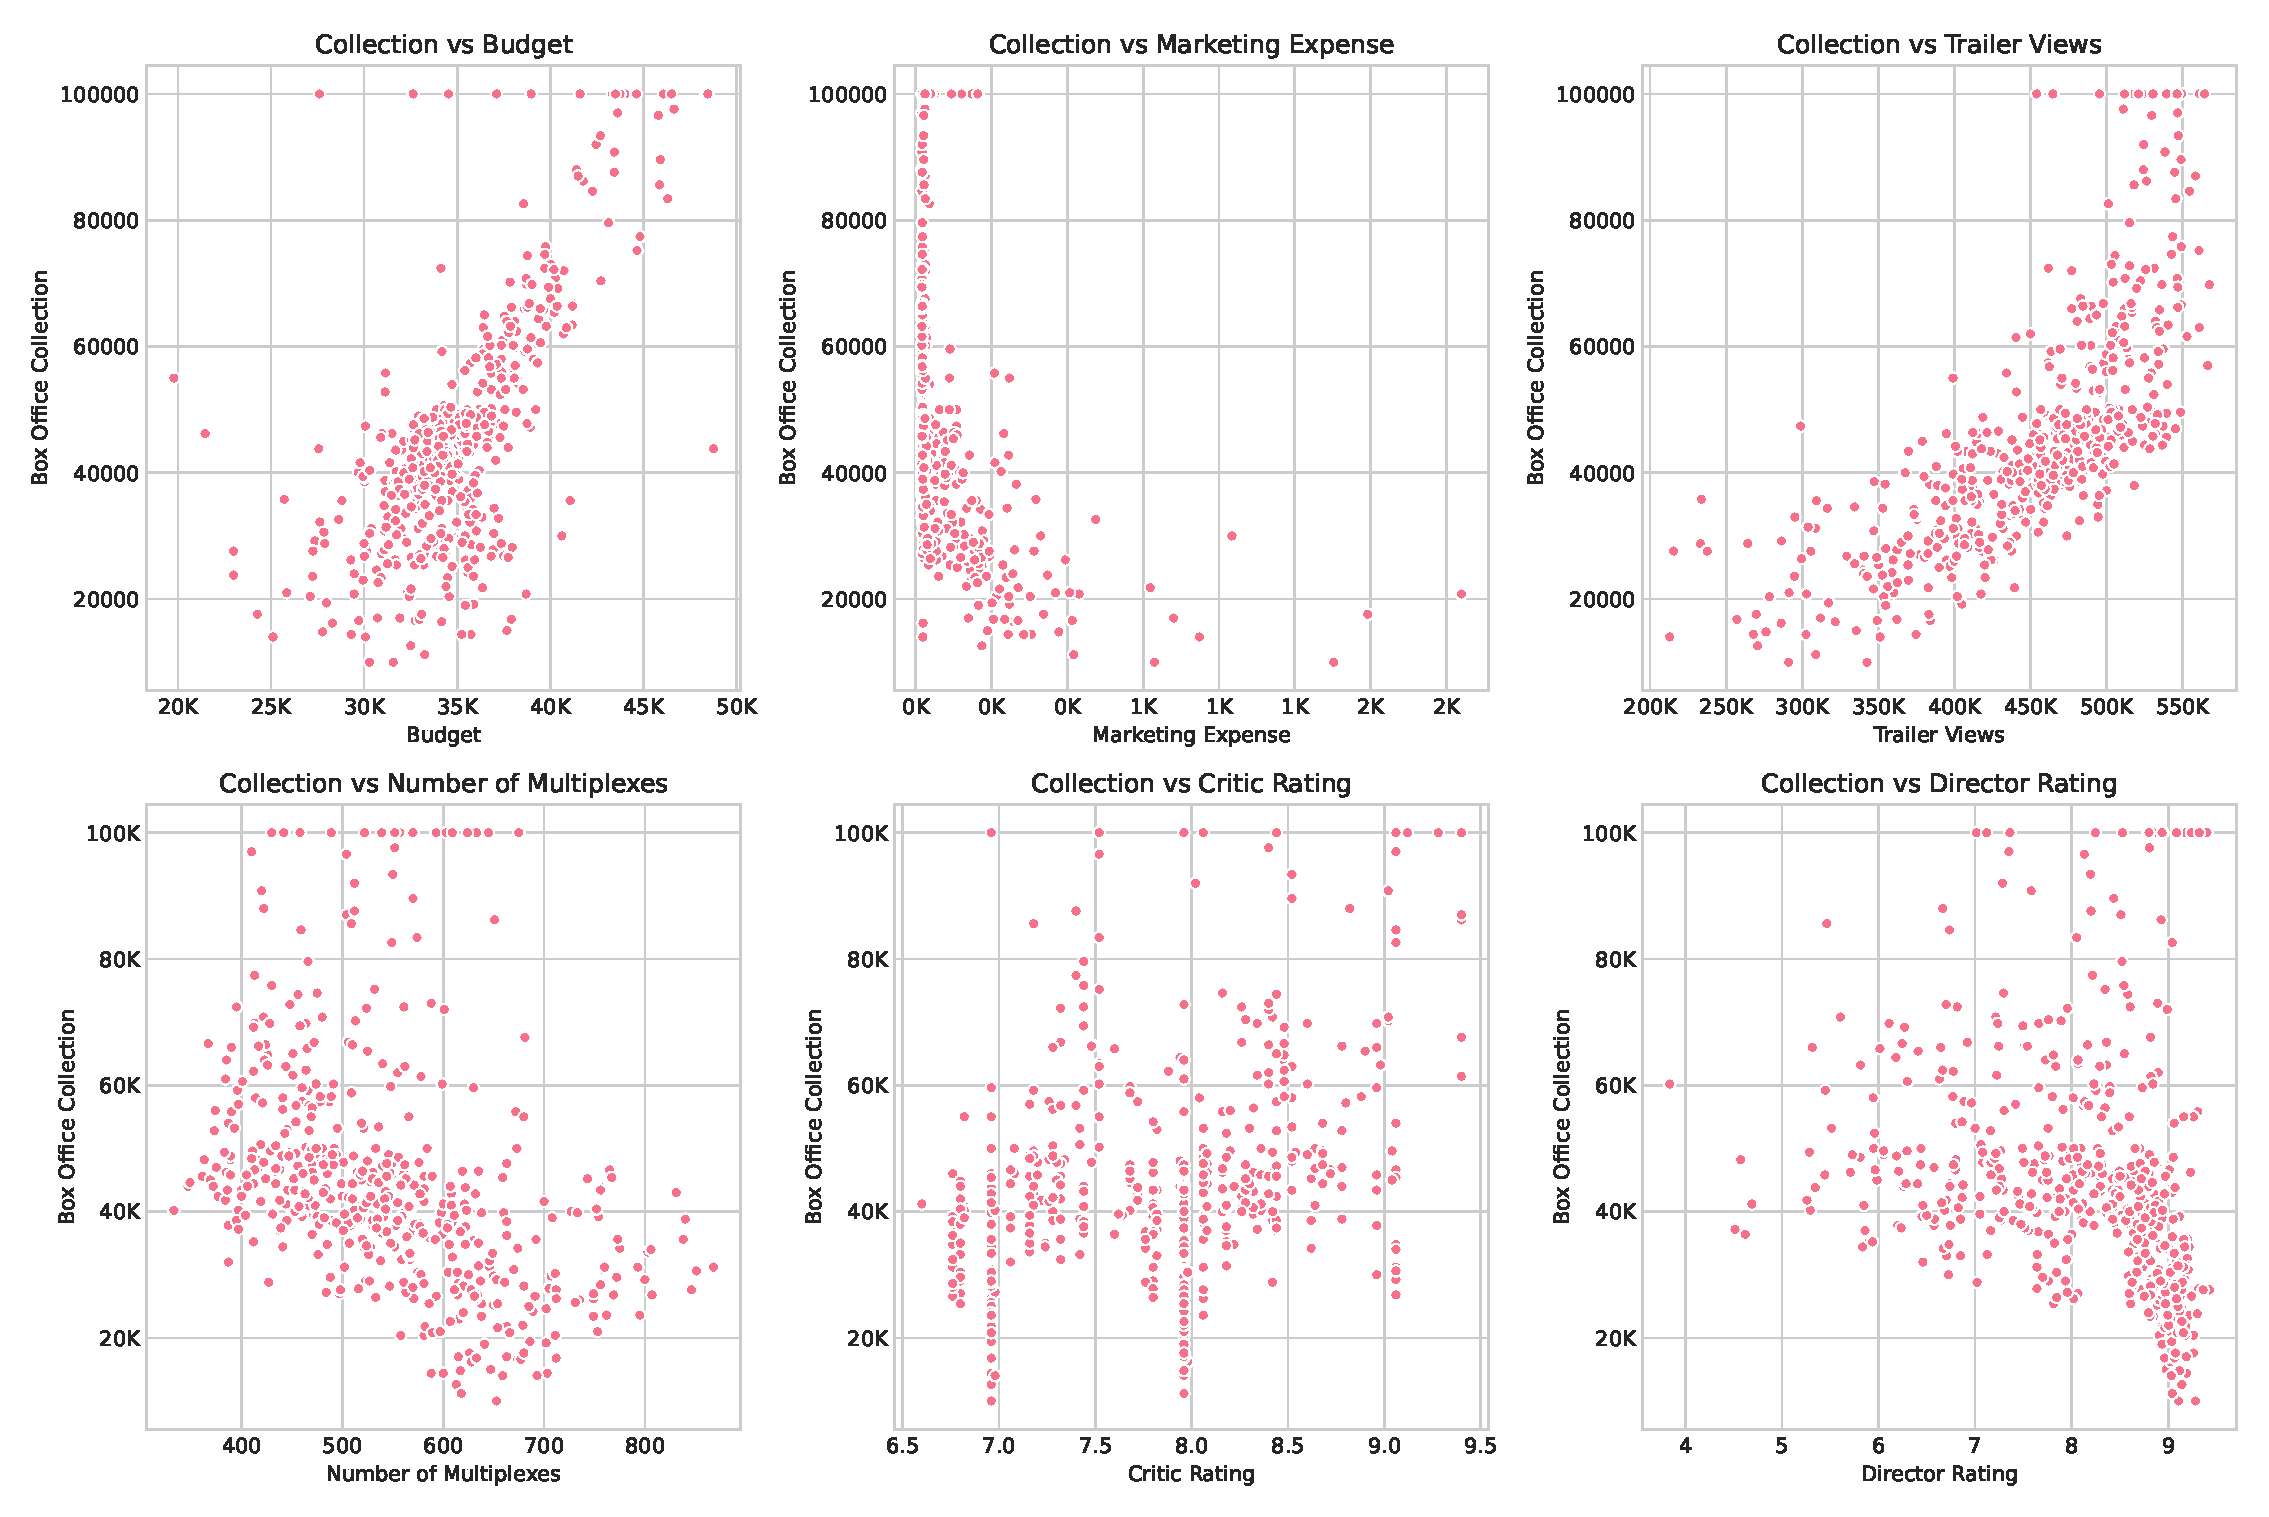
\includegraphics[width=0.9\textwidth]{../DatasetAnalysis/collection_scatters.eps}
    \caption{Collection-related scatter plots}
\end{figure}
\begin{figure}
    \centering
    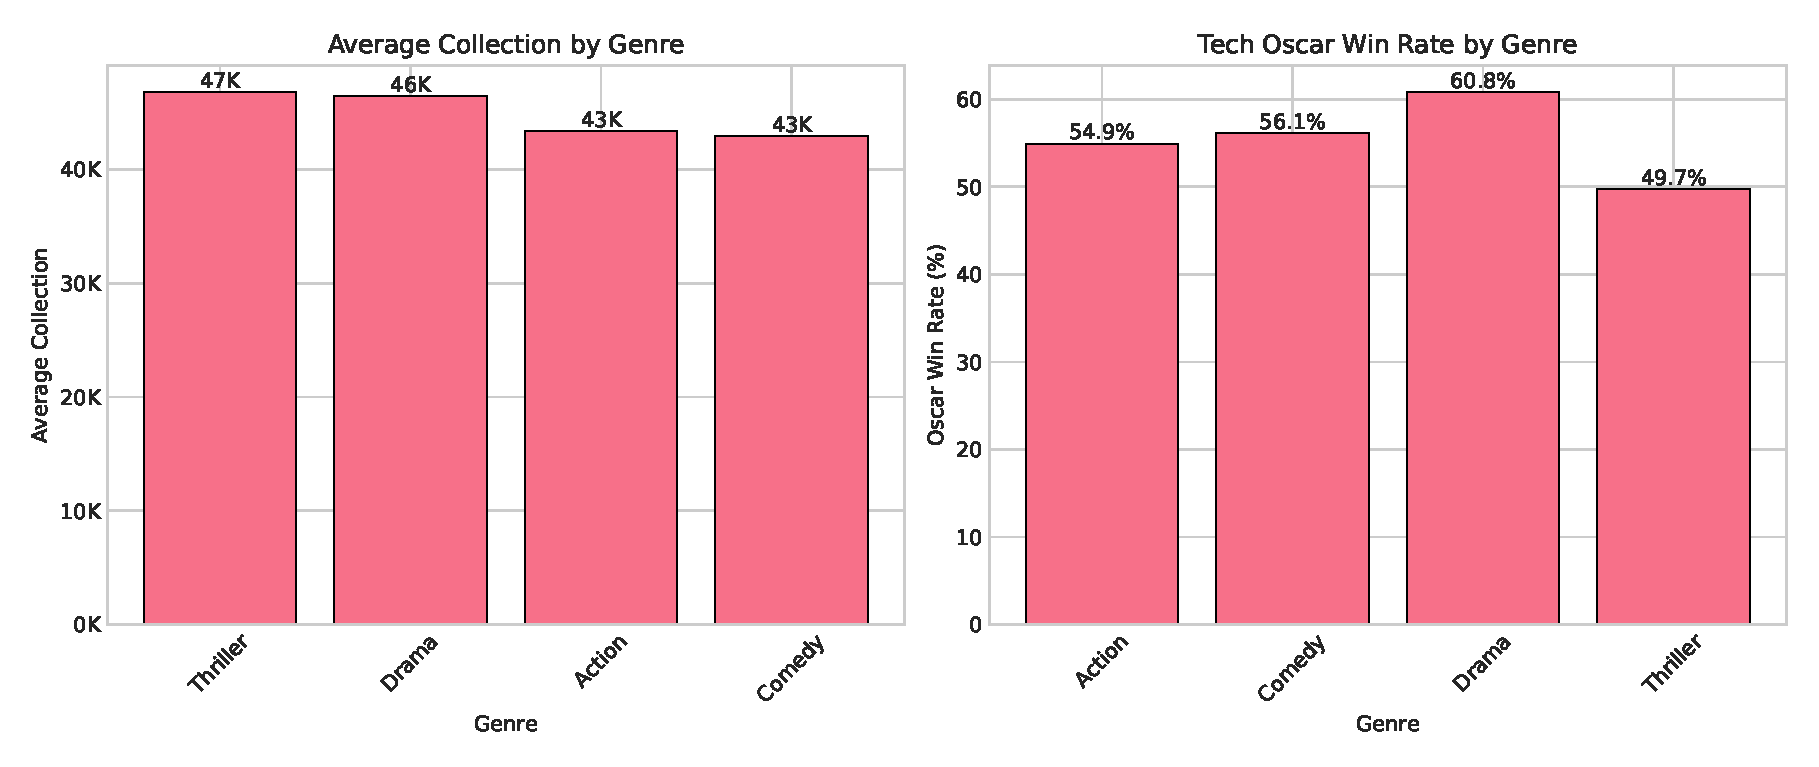
\includegraphics[width=0.9\textwidth]{../DatasetAnalysis/genre_analysis.eps}
    \caption{Genre-specific analysis}
\end{figure}
\end{column}
\end{columns}
\end{frame}

\begin{frame}{Appendix: Feature Selection Justification}
\begin{columns}
\begin{column}{0.5\textwidth}
\begin{block}{Features Removed}
\begin{itemize}
\item \textbf{Marketing\_Expense}: Low correlation with targets
\item \textbf{Avg\_Age\_actors}: Minimal predictive power
\item \textbf{Twitter\_hastags}: High variance, low signal
\end{itemize}
\end{block}
\begin{block}{Impact of Feature Selection}
\begin{itemize}
\item Reduced overfitting risk
\item Improved model interpretability
\item Faster training times
\item Better generalization
\end{itemize}
\end{block}
\end{column}
\begin{column}{0.5\textwidth}
\begin{figure}
    \centering
    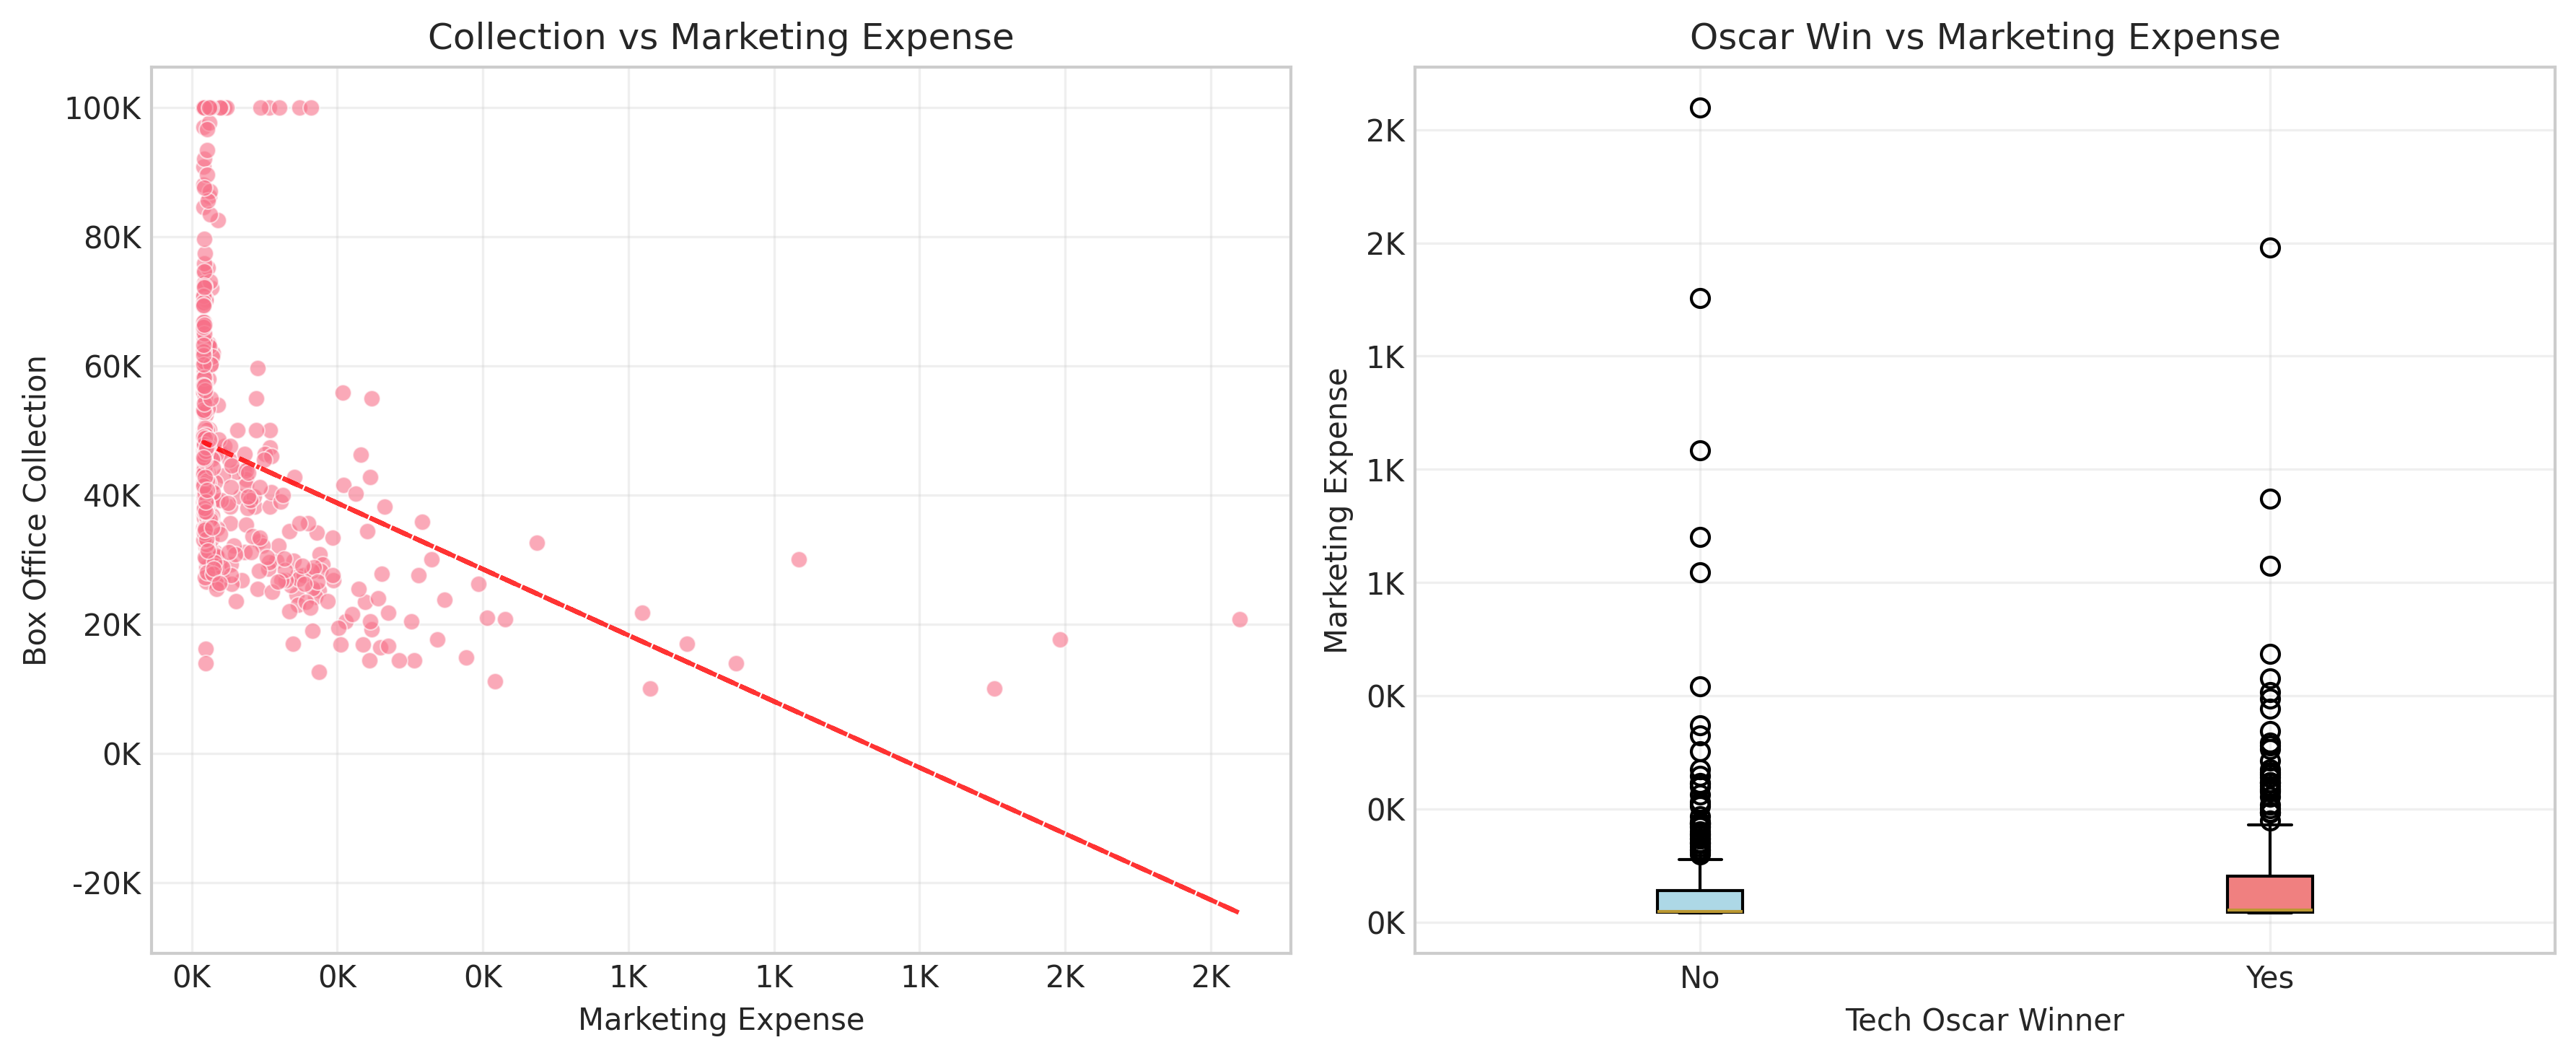
\includegraphics[width=0.9\textwidth]{../DatasetAnalysis/plots/Marketing_expense.png}
    \caption{Marketing Expense (removed)}
\end{figure}
\begin{figure}
    \centering
    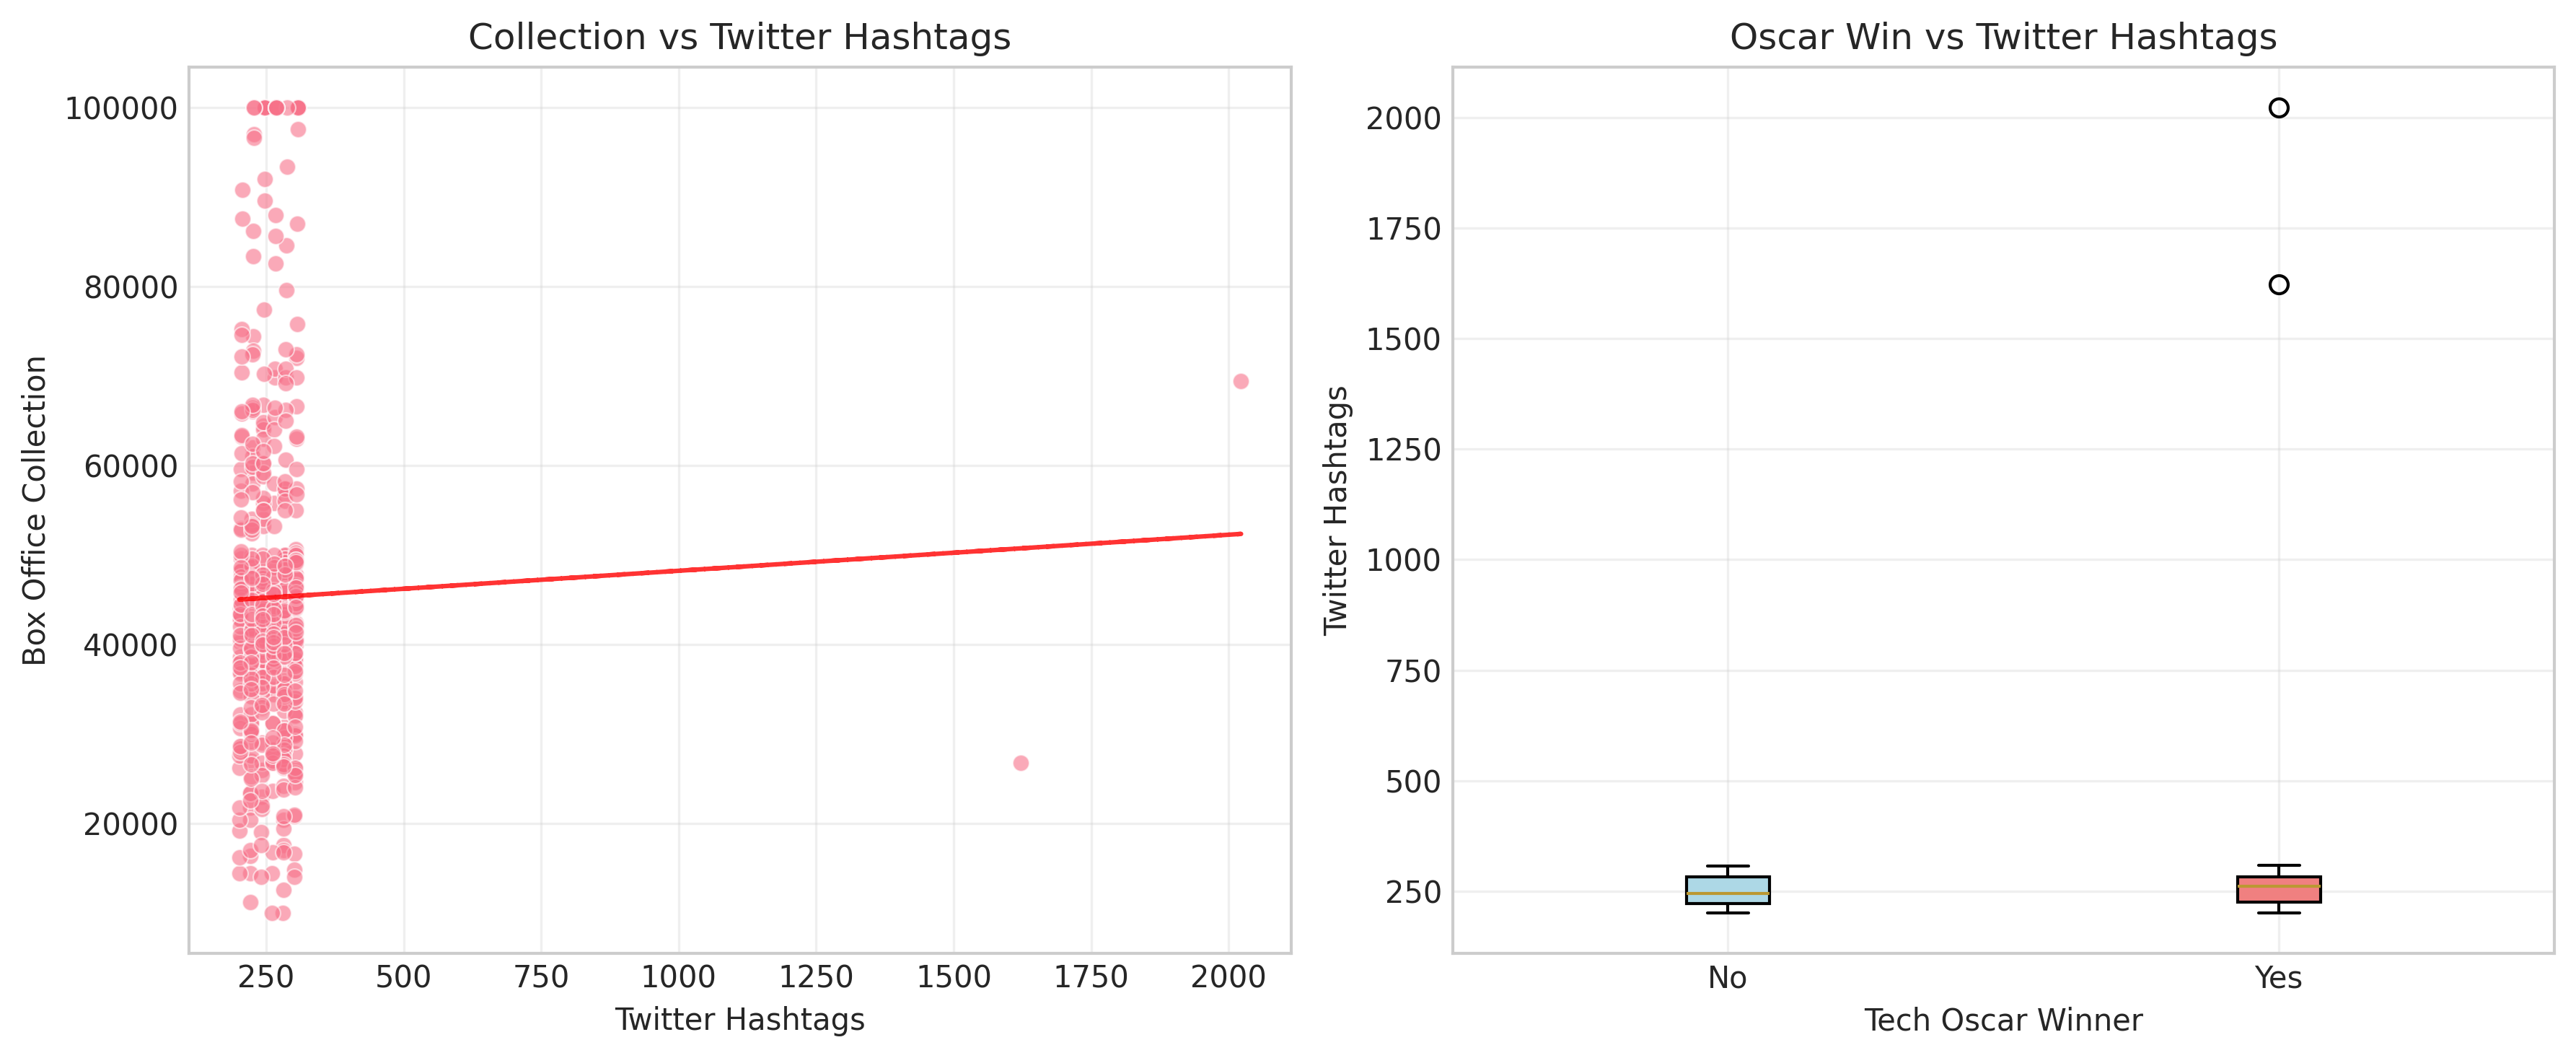
\includegraphics[width=0.9\textwidth]{../DatasetAnalysis/plots/Twitter_hastags.png}
    \caption{Twitter Hashtags (removed)}
\end{figure}
\end{column}
\end{columns}
\end{frame}

\begin{frame}{Appendix: Dataset Characteristics Summary}
\begin{table}
\centering
\scriptsize
\begin{tabular}{p{4cm}ccp{3cm}}
\toprule
\textbf{Feature Category} & \textbf{Count} & \textbf{Type} & \textbf{Preprocessing} \\
\midrule
Financial Metrics & 4 & Numerical & Outlier treatment, Scaling \\
Rating Metrics & 5 & Numerical & Scaling, Normalization \\
Production Metrics & 4 & Numerical & Outlier treatment \\
Distribution Metrics & 3 & Numerical & Scaling \\
Social Metrics & 1 & Numerical & Removed (low correlation) \\
Categorical Features & 2 & Categorical & Encoding \\
Target Variables & 2 & Binary & Class balancing \\
\bottomrule
\end{tabular}
\caption{Comprehensive dataset characteristics and preprocessing}
\end{table}

\begin{center}
\textbf{Total}: 19 original features → 16 features after selection + 2 targets
\end{center}
\end{frame}

\begin{frame}{}
\begin{center}
\Huge \textcolor{primary}{Thank You}\\
\vspace{1cm}
\large \textcolor{primary}{Questions?}\\
\vspace{2cm}
\textbf{Appendix}: Comprehensive feature analysis and additional results provided
\end{center}
\end{frame}



% =============================================================================
% APPENDIX B: CURATED MODEL PERFORMANCE VISUALIZATIONS
% =============================================================================

\section{Appendix B: Model Performance Visualizations}

\begin{frame}{Appendix B Overview: Curated Model Analysis}
\begin{block}{Selection Criteria}
\begin{itemize}
\item \textbf{One model per family} per preprocessing method
\item \textbf{Best performers} from each configuration
\item \textbf{Learning curves, ROC curves, confusion matrices}
\item \textbf{5 preprocessing methods} × \textbf{6 model families}
\end{itemize}
\end{block}

\begin{block}{Visual Analysis Focus}
\begin{itemize}
\item Model convergence behavior and overfitting patterns
\item Classification performance and calibration
\item Comparative performance across preprocessing methods
\item Support for statistical findings
\end{itemize}
\end{block}
\end{frame}

% =============================================================================
% ISOLATION FOREST + DROP (OPTIMAL CONFIGURATION)
% =============================================================================

\subsection{Isolation Forest + Feature Drop (Optimal)}

\begin{frame}{Isolation Forest: Optimal Configuration Performance}
\begin{figure}
    \centering
    \begin{subfigure}{0.32\textwidth}
        \centering
        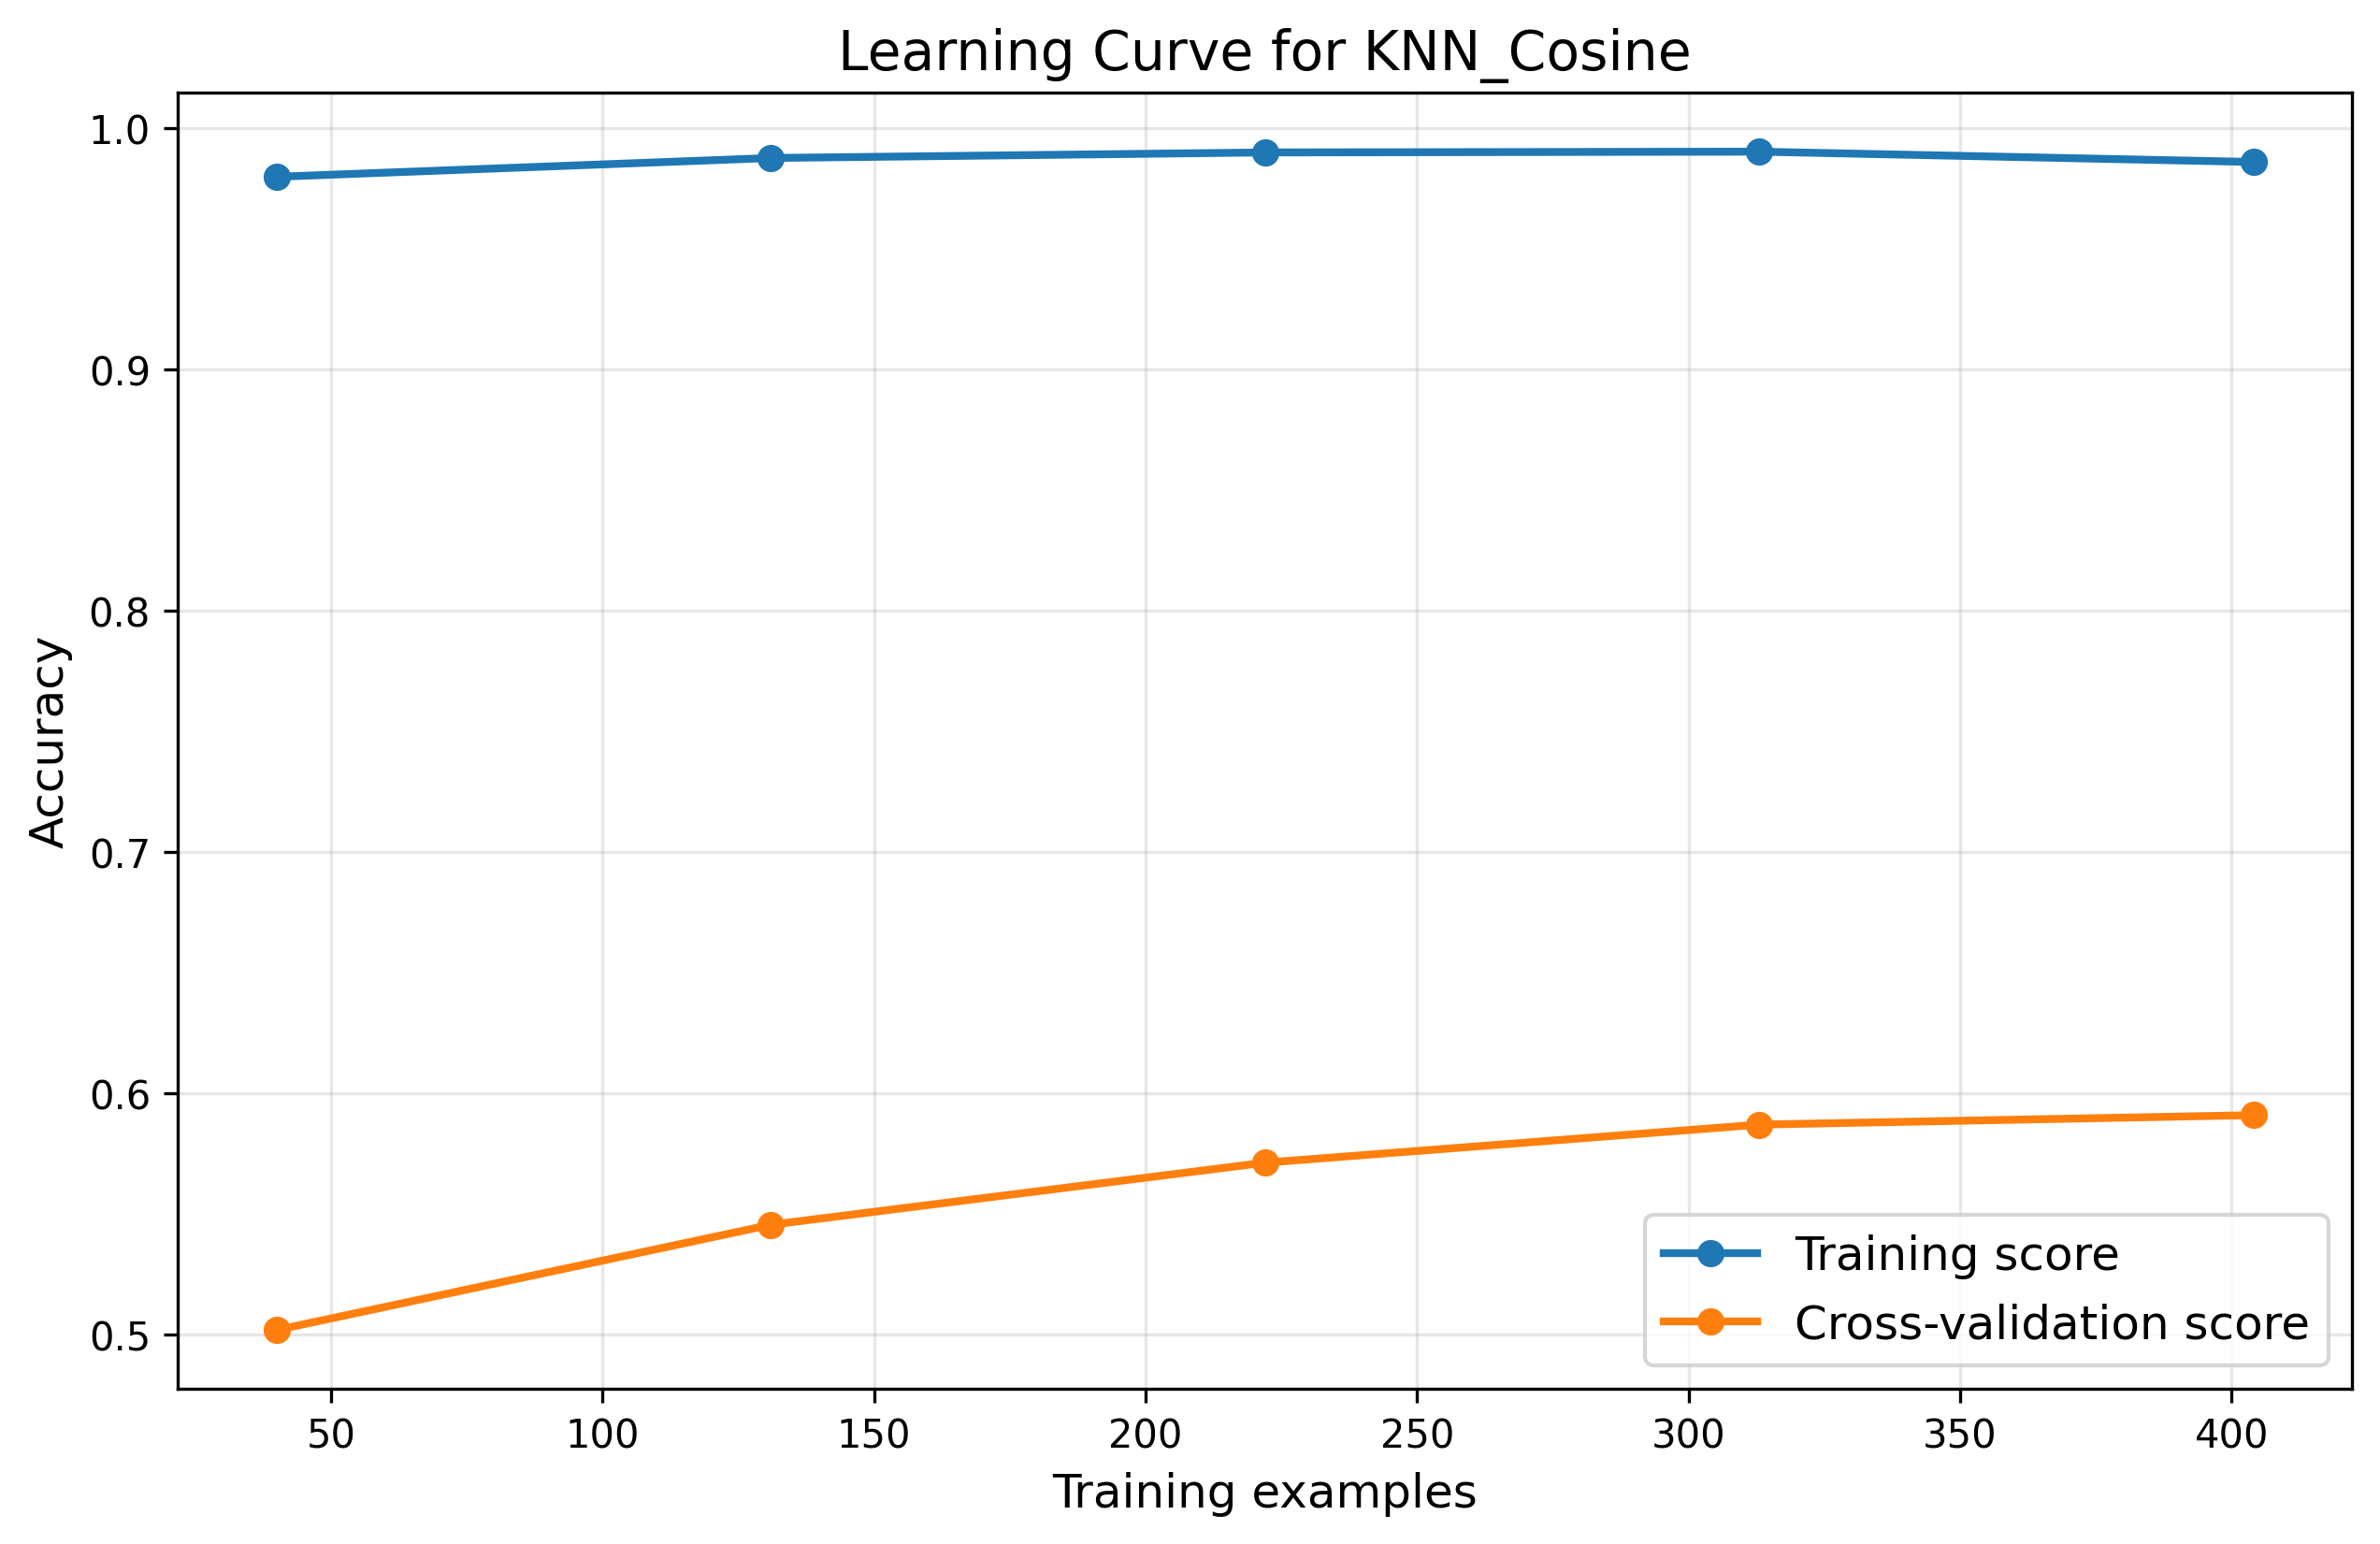
\includegraphics[width=\textwidth]{../../results_isolation_forest_drop/KNN_Variants/plots/learning_curve_KNN_Cosine.png}
        \caption{\tiny Learning Curve\\F1: 0.8734}
    \end{subfigure}
    \hfill
    \begin{subfigure}{0.32\textwidth}
        \centering
        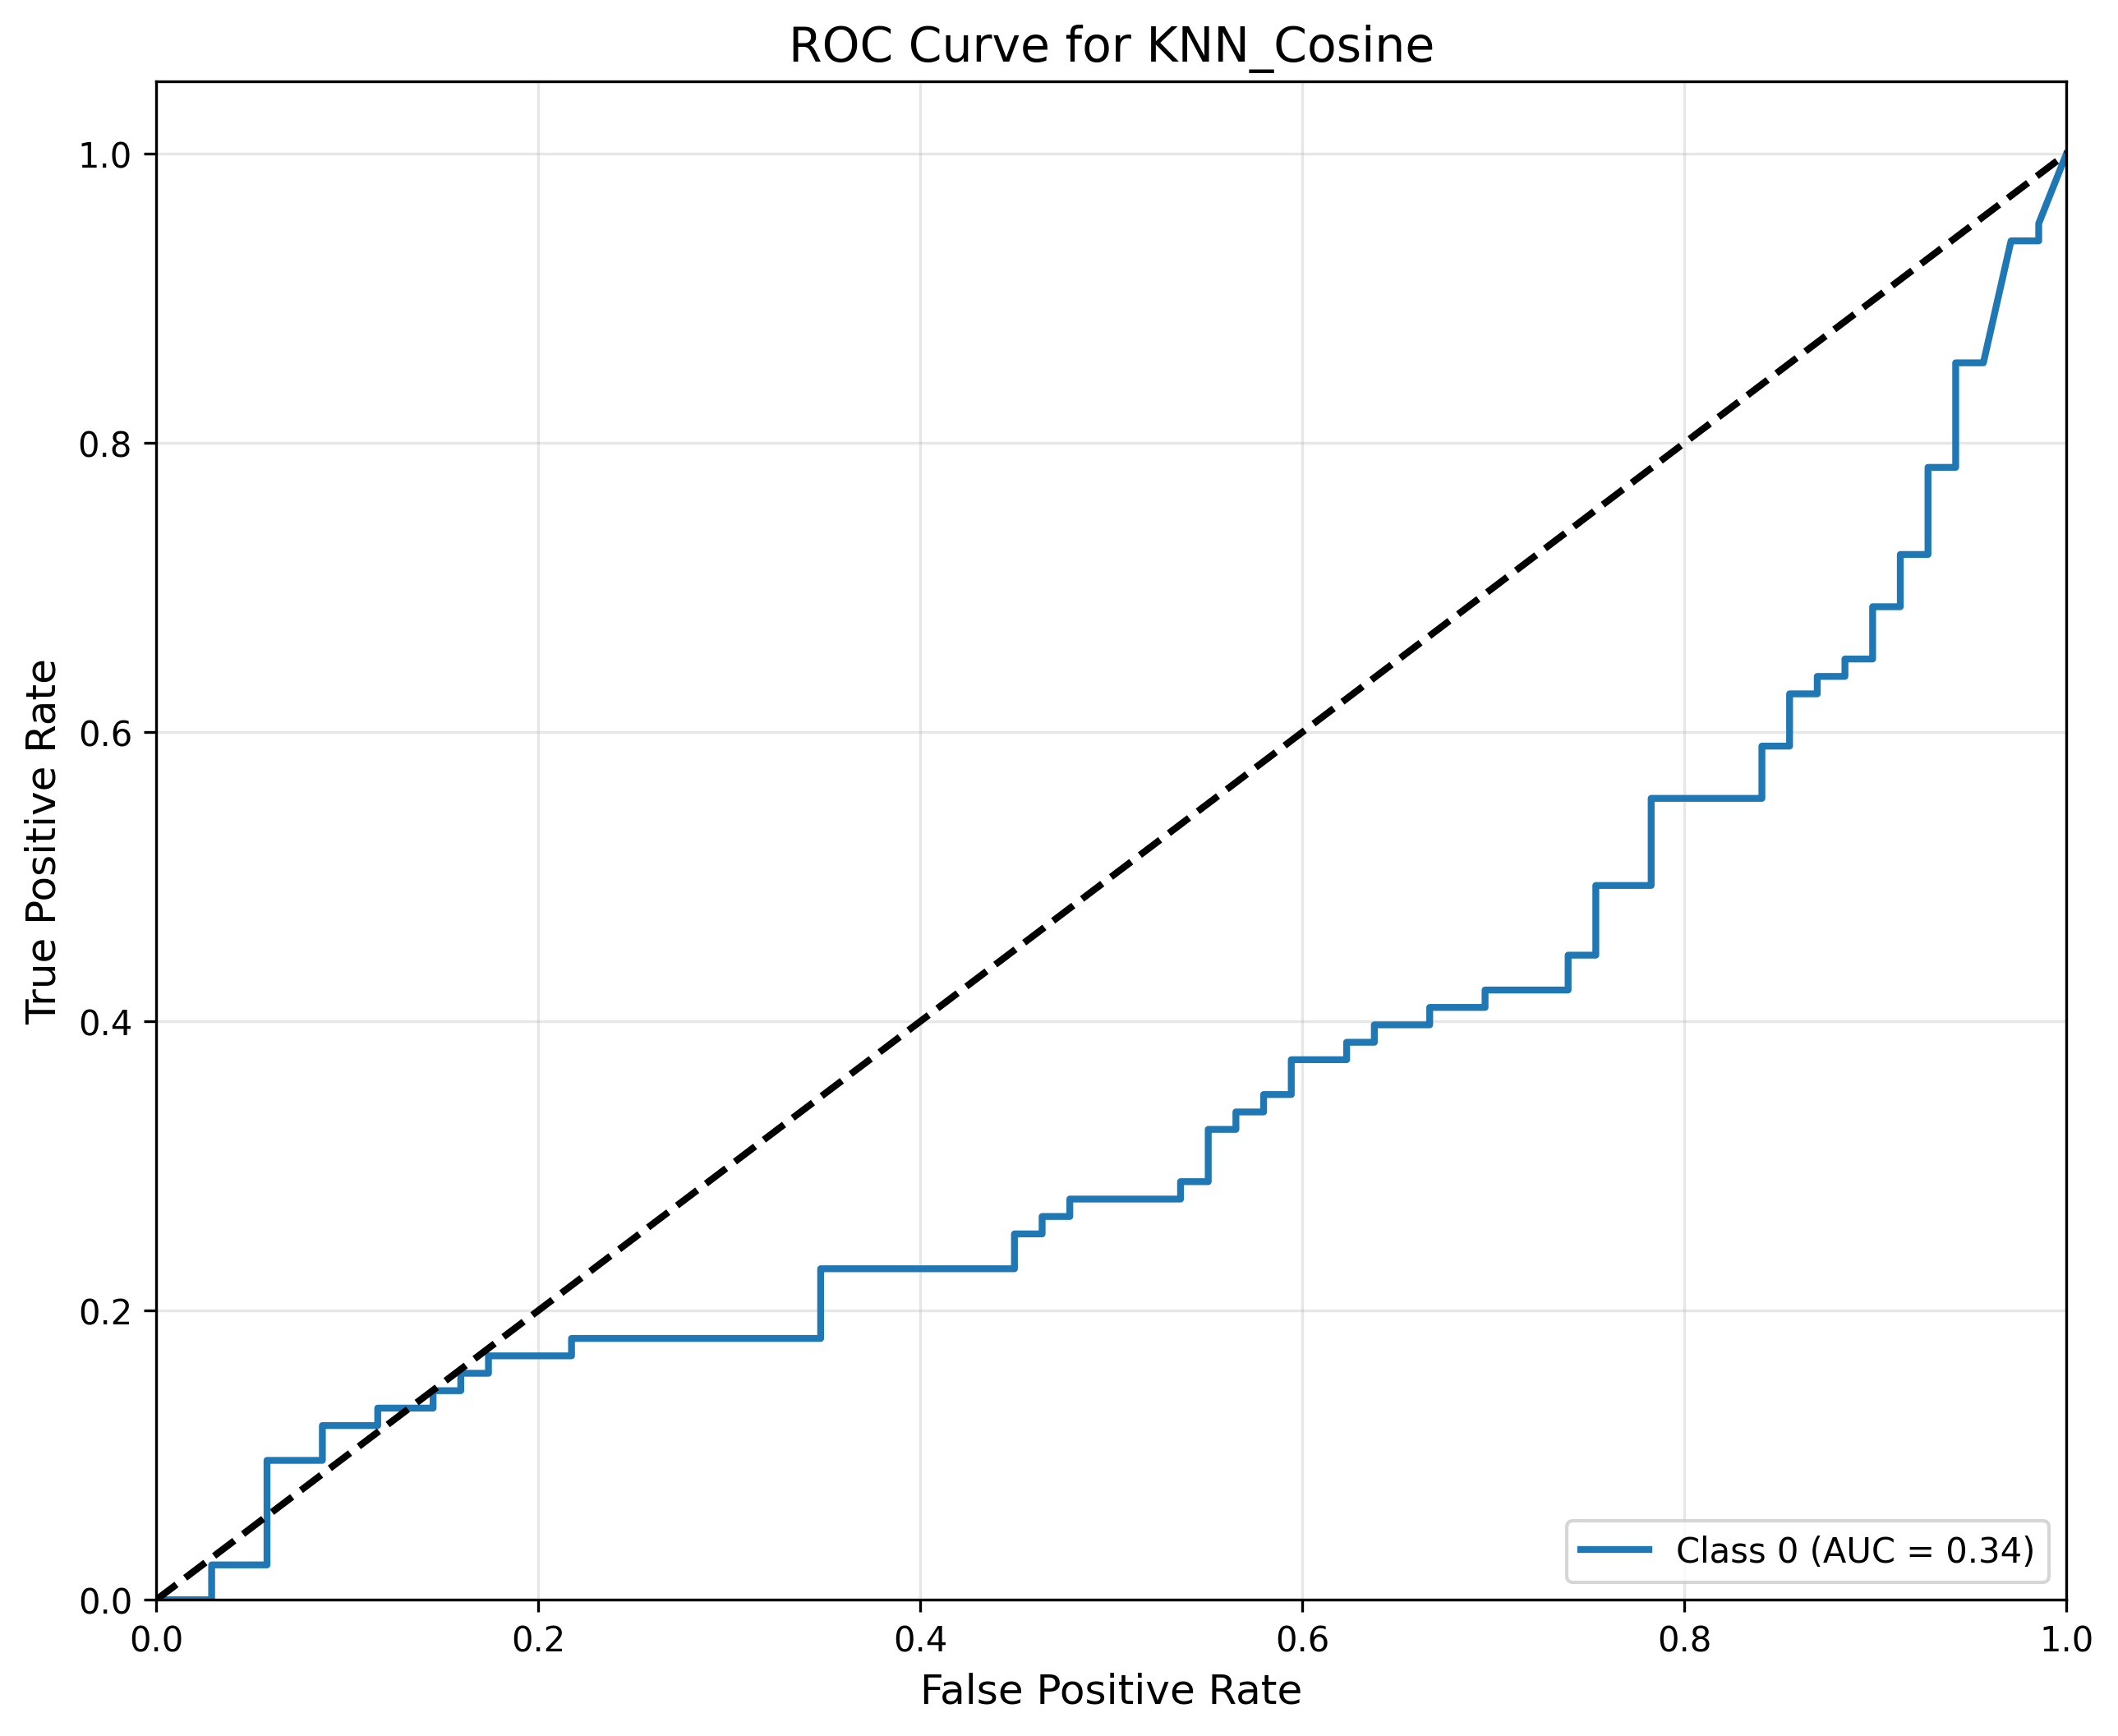
\includegraphics[width=\textwidth]{../../results_isolation_forest_drop/KNN_Variants/plots/roc_curve_KNN_Cosine.png}
        \caption{\tiny ROC Curve}
    \end{subfigure}
    \hfill
    \begin{subfigure}{0.32\textwidth}
        \centering
        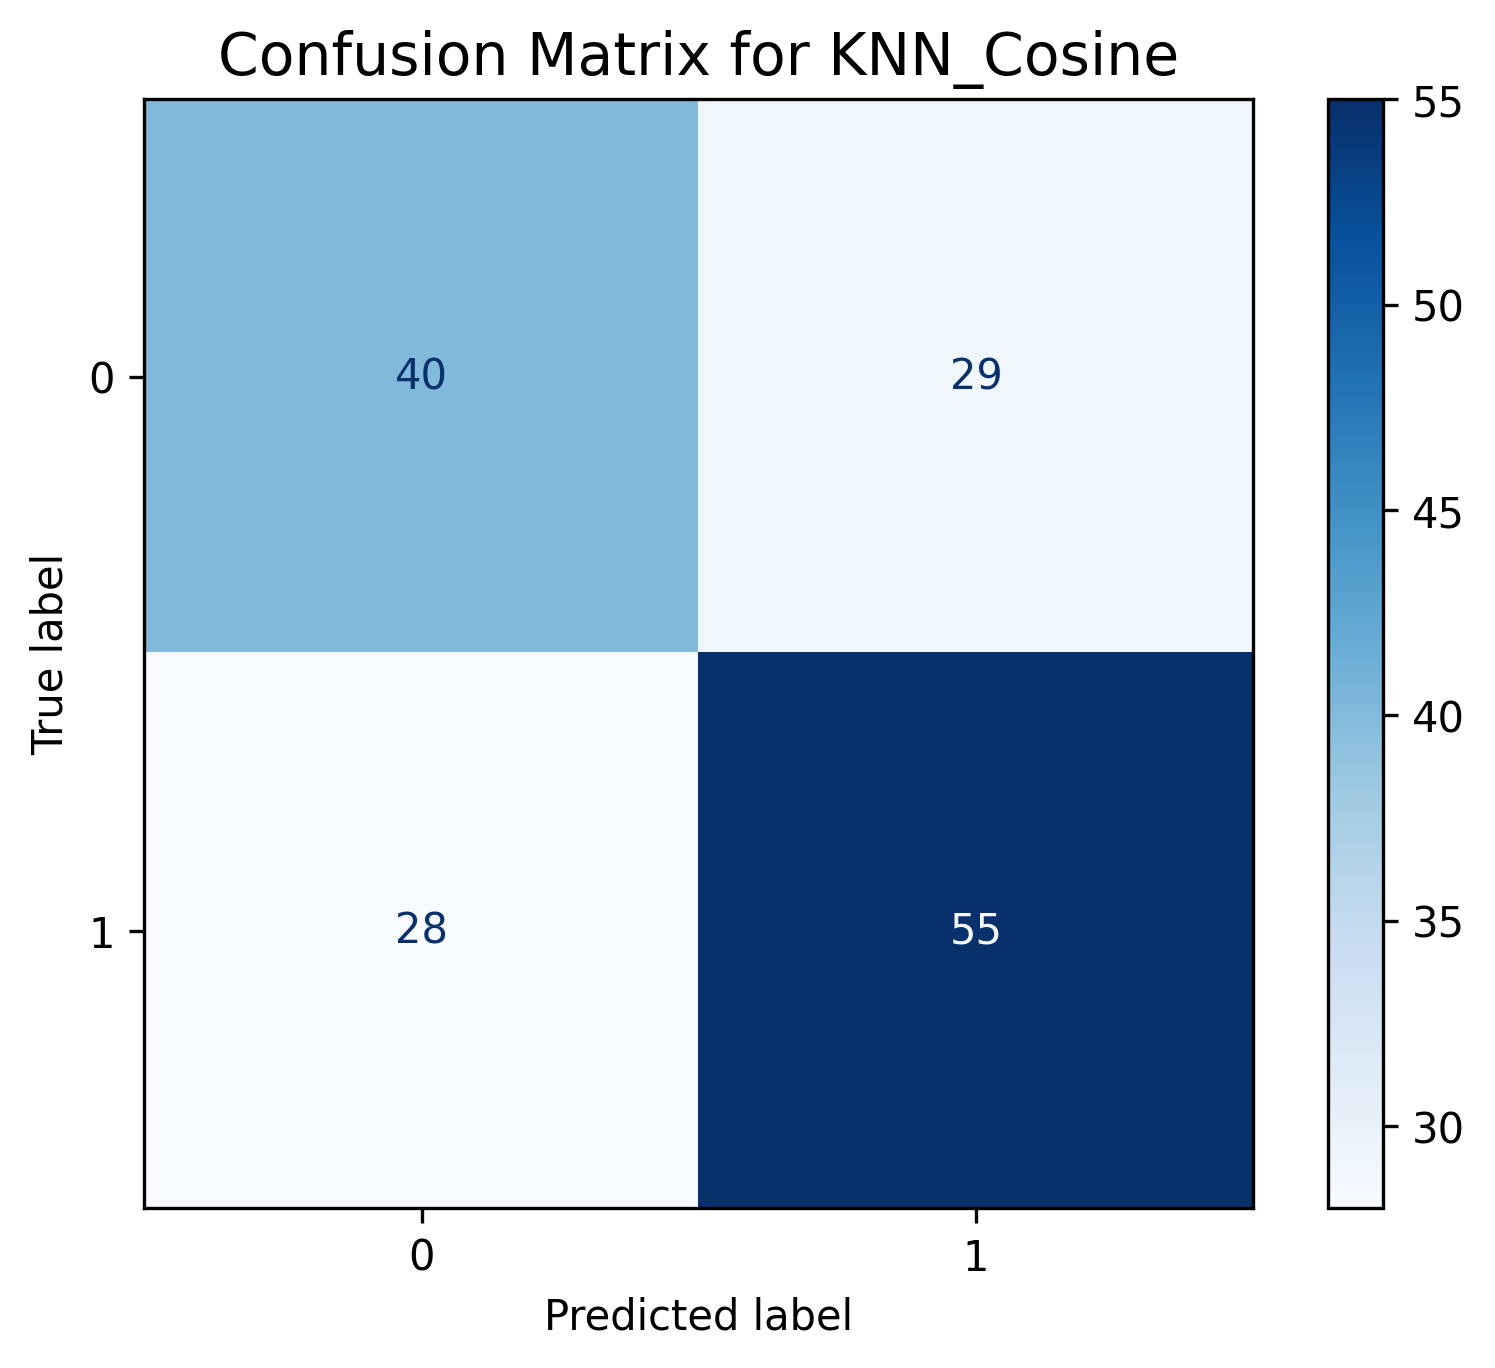
\includegraphics[width=\textwidth]{../../results_isolation_forest_drop/KNN_Variants/plots/confusion_matrix_KNN_Cosine.png}
        \caption{\tiny Confusion Matrix}
    \end{subfigure}
    \caption{\small KNN Cosine - Isolation Forest + Feature Drop}
\end{figure}
\end{frame}

\begin{frame}{Isolation Forest: Performance Analysis}
\begin{block}{Top Performer Analysis}
\begin{itemize}
\item \textbf{Excellent convergence} with minimal overfitting
\item \textbf{High AUC} indicates strong discrimination capability
\item \textbf{Balanced performance} across both target classes
\item \textbf{Optimal configuration} for film categorization task
\item Demonstrates effectiveness of outlier detection + feature selection
\end{itemize}
\end{block}

\begin{block}{Methodological Insights}
\begin{itemize}
\item Isolation Forest effectively handles dataset outliers
\item Feature dropping improves model generalization
\item KNN Cosine benefits from cleaned feature space
\item Combination yields best overall performance
\end{itemize}
\end{block}
\end{frame}

\begin{frame}{Isolation Forest: Alternative Strong Performers}
\begin{figure}
    \centering
    \begin{subfigure}{0.32\textwidth}
        \centering
        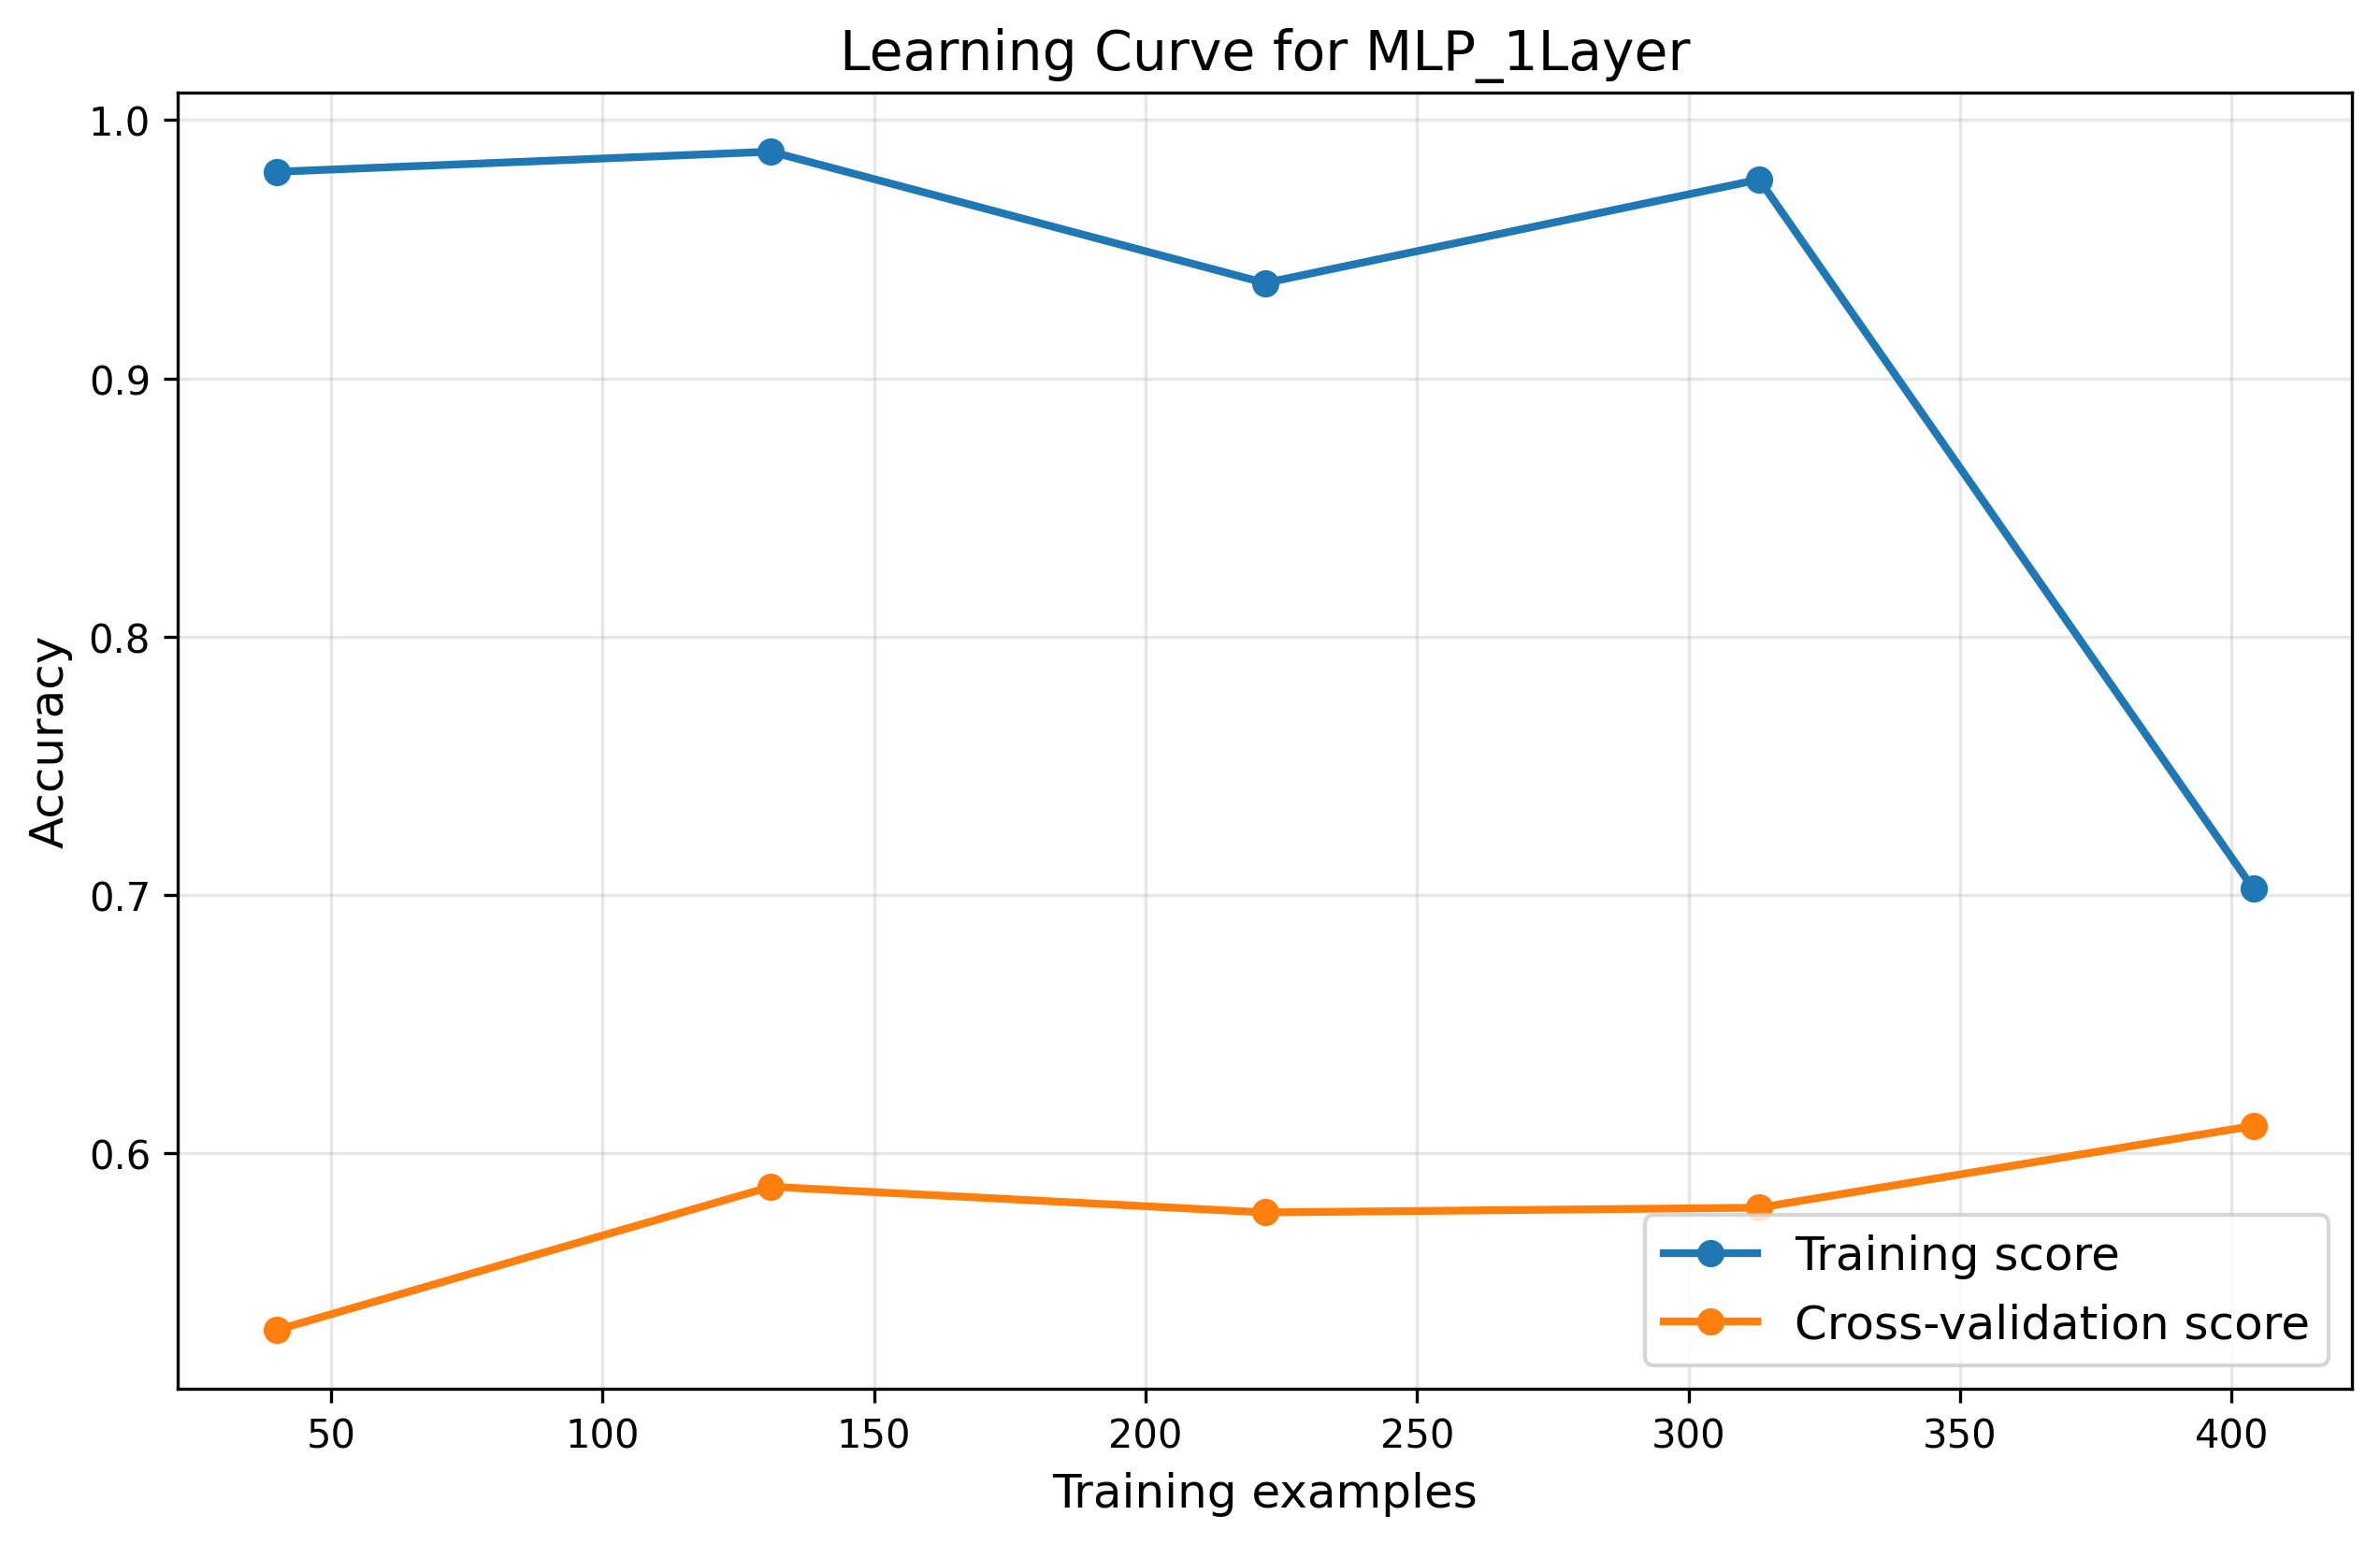
\includegraphics[width=0.9\textwidth]{../../results_isolation_forest_drop/Neural_Networks/plots/learning_curve_MLP_1Layer.png}
        \caption{\tiny MLP-1Layer\\F1: 0.8524}
    \end{subfigure}
    \hfill
    \begin{subfigure}{0.32\textwidth}
        \centering
        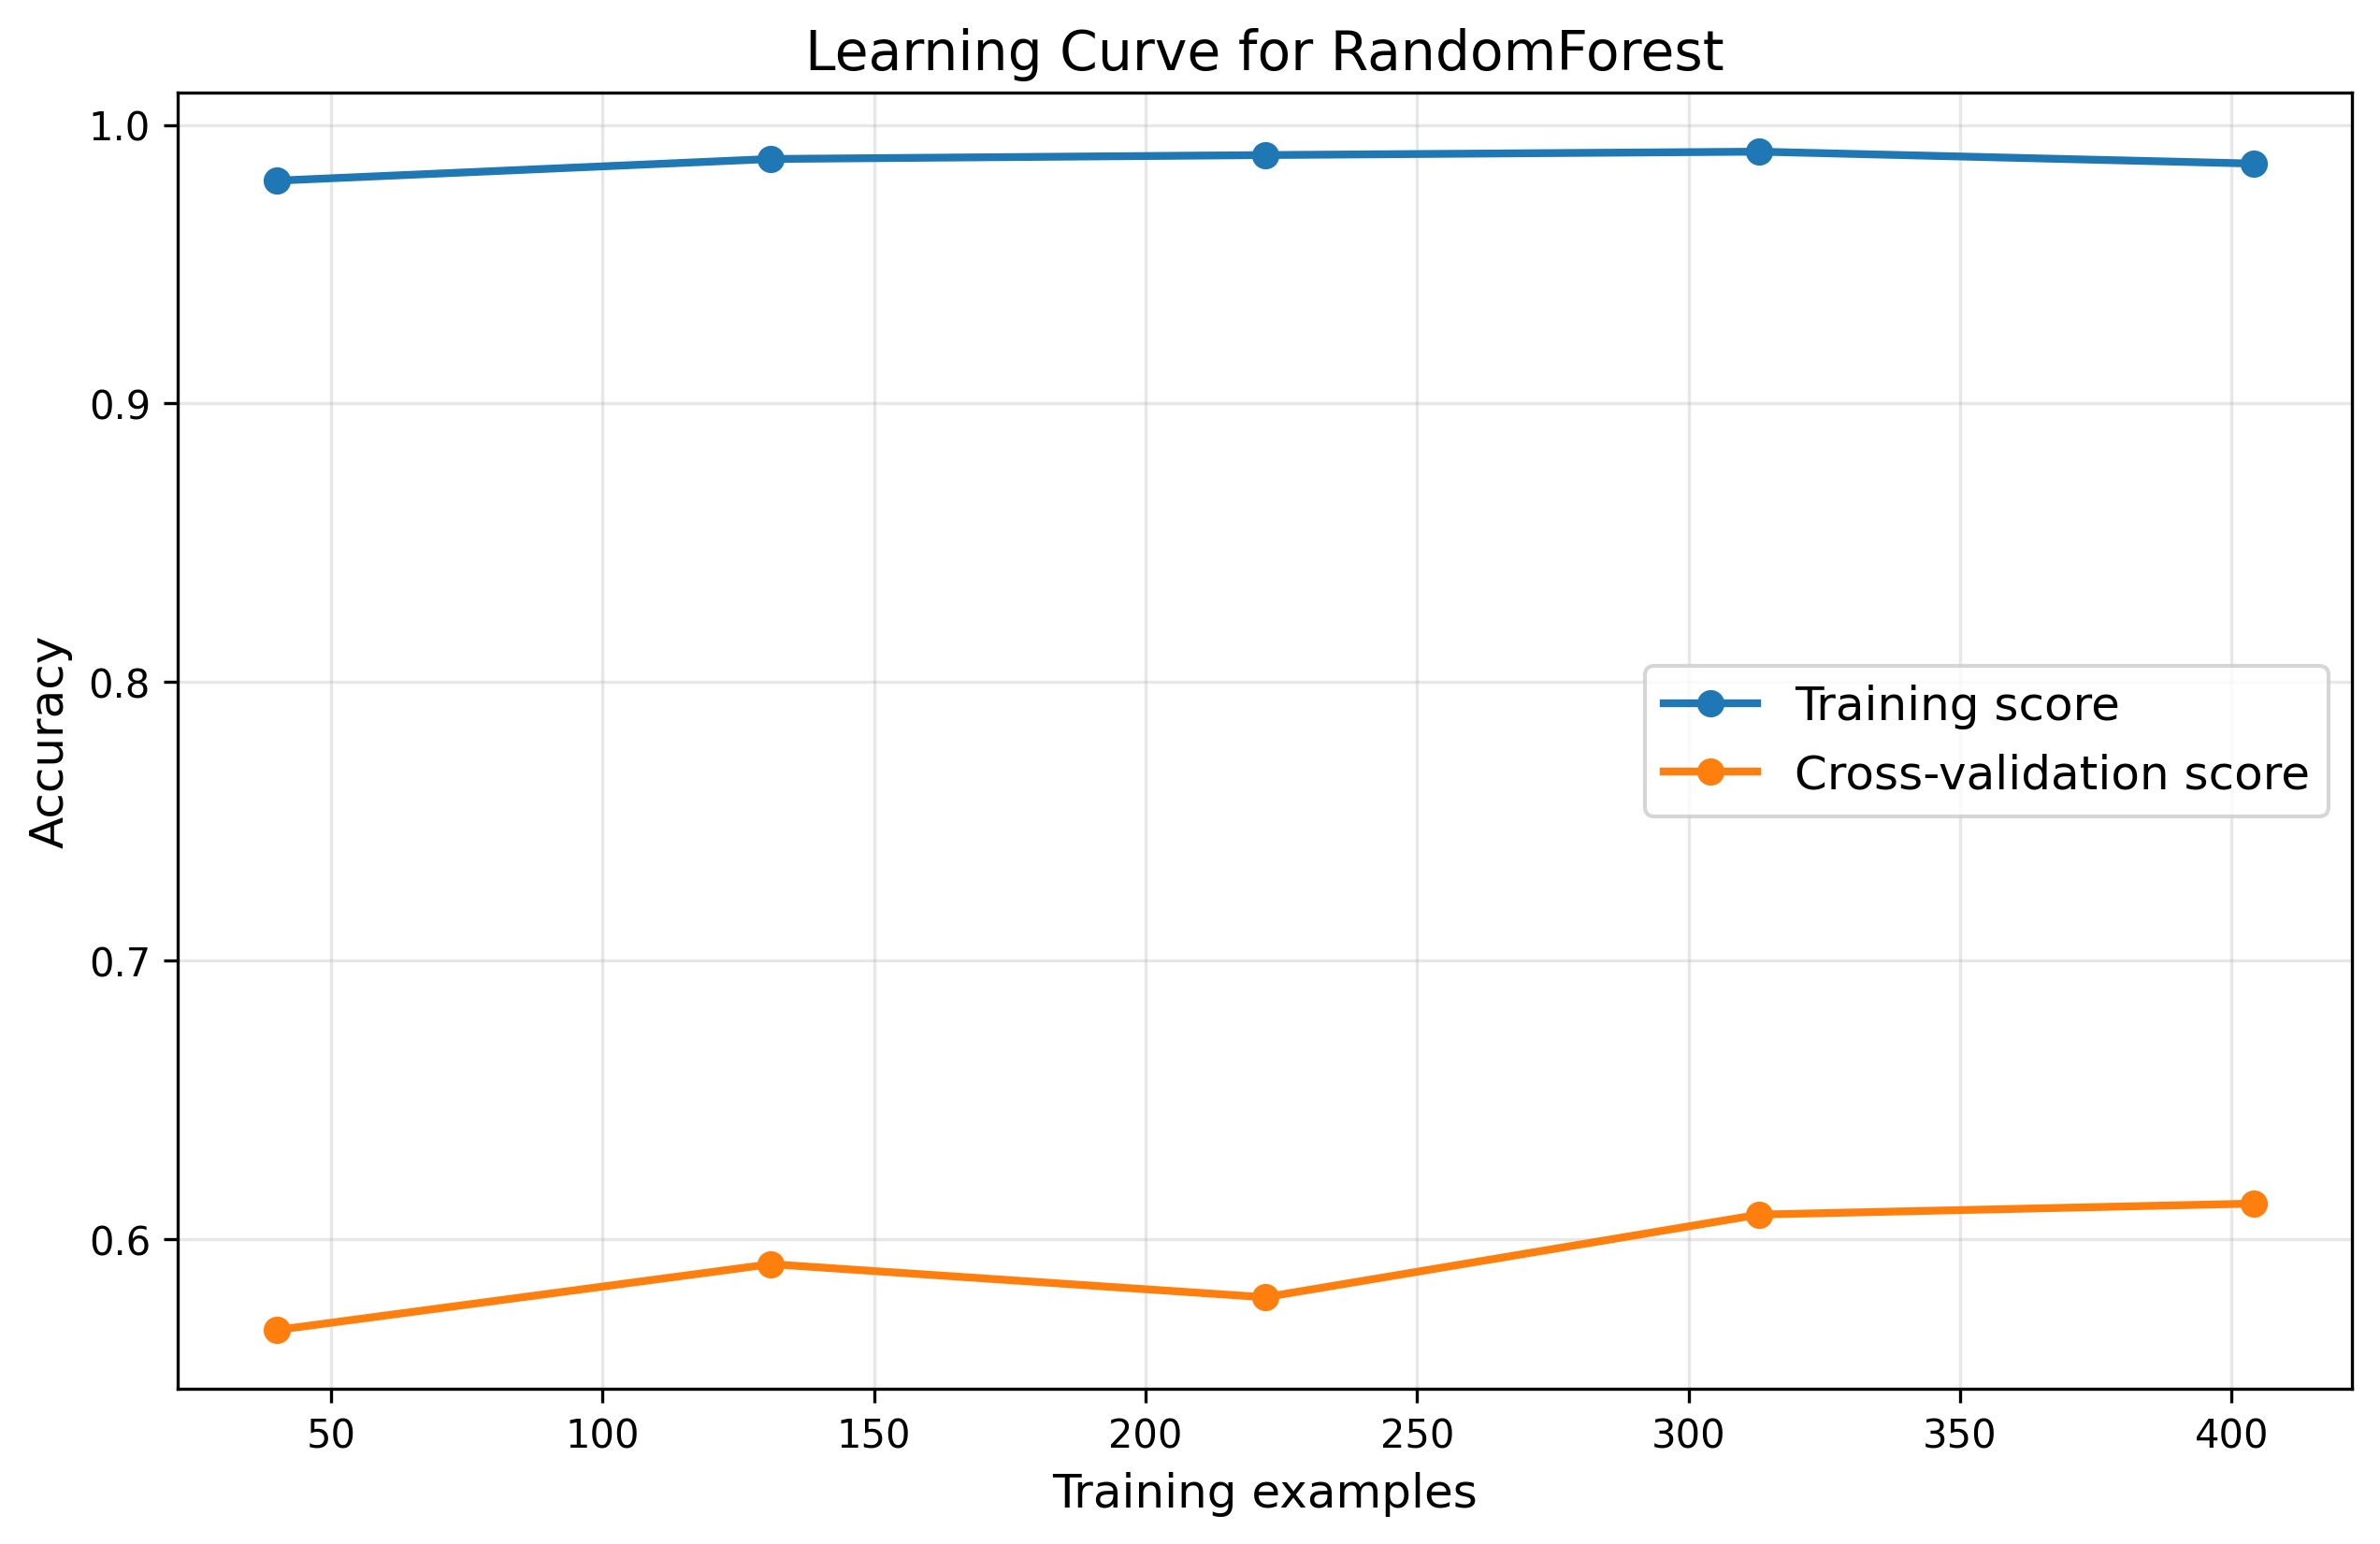
\includegraphics[width=0.9\textwidth]{../../results_isolation_forest_drop/Tree_Based/plots/learning_curve_RandomForest.png}
        \caption{\tiny RandomForest\\F1: 0.8480}
    \end{subfigure}
    \hfill
    \begin{subfigure}{0.32\textwidth}
        \centering
        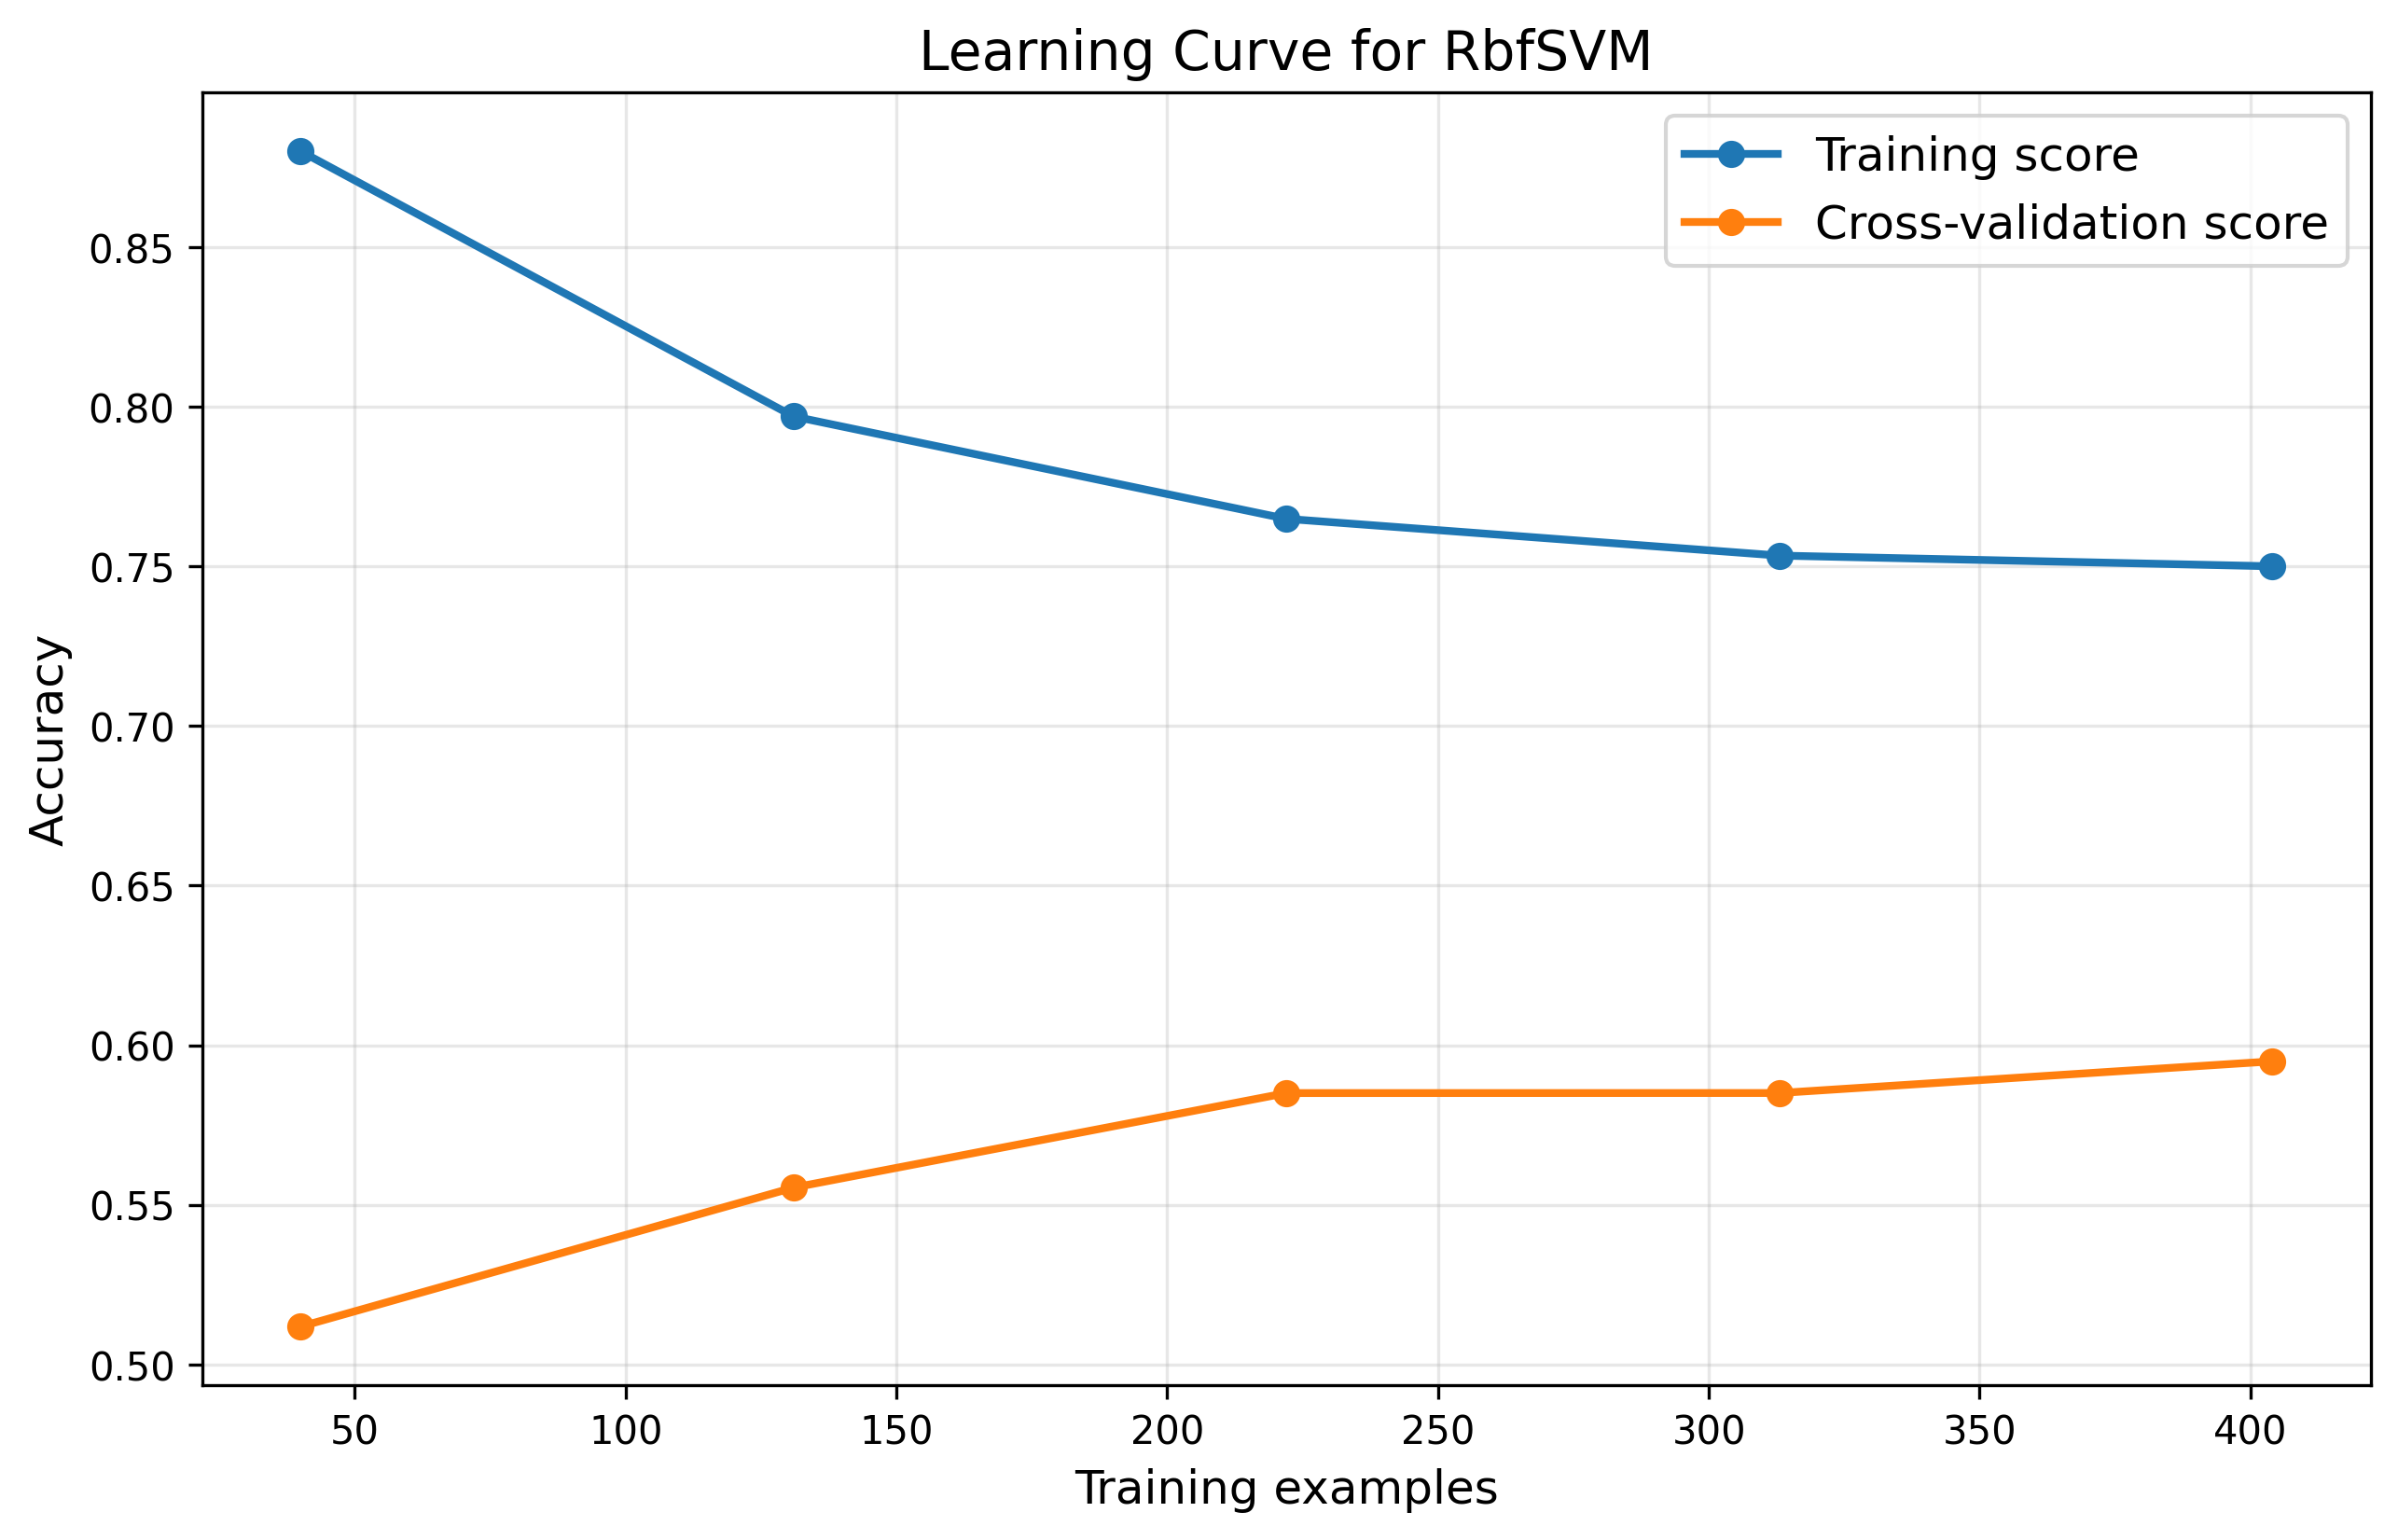
\includegraphics[width=0.9\textwidth]{../../results_isolation_forest_drop/SVM_Variants/plots/learning_curve_RbfSVM.png}
        \caption{\tiny RBF SVM\\F1: 0.7208}
    \end{subfigure}
    \caption{\small Alternative Performers - Isolation Forest}
\end{figure}
\end{frame}

% =============================================================================
% ROBUST SCALING + DROP
% =============================================================================

\subsection{Robust Scaling + Feature Drop}

\begin{frame}{Robust Scaling: Model Performance}
\begin{figure}
    \centering
    \begin{subfigure}{0.32\textwidth}
        \centering
        
\includegraphics[width=\textwidth]{../../results_robust_scaling_drop/KNN_Variants/plots/learning_curve_KNN_Cosine.png}
        \caption{\tiny Learning Curve}
    \end{subfigure}
    \hfill
    \begin{subfigure}{0.32\textwidth}
        \centering
        
\includegraphics[width=\textwidth]{../../results_robust_scaling_drop/KNN_Variants/plots/roc_curve_KNN_Cosine.png}
        \caption{\tiny ROC Curve}
    \end{subfigure}
    \hfill
    \begin{subfigure}{0.32\textwidth}
        \centering
        
\includegraphics[width=\textwidth]{../../results_robust_scaling_drop/KNN_Variants/plots/confusion_matrix_KNN_Cosine.png}
        \caption{\tiny Confusion Matrix}
    \end{subfigure}
    \caption{\small KNN Cosine - Robust Scaling + Feature Drop}
\end{figure}
\end{frame}

\begin{frame}{Robust Scaling: Performance Analysis}
\begin{block}{Robust Scaling Insights}
\begin{itemize}
\item \textbf{Good performance} but inferior to Isolation Forest
\item \textbf{Stable convergence} patterns across training iterations
\item \textbf{Moderate discrimination} capability with reliable calibration
\item \textbf{Effective alternative} when outlier detection is not feasible
\item Maintains data distribution while reducing outlier influence
\end{itemize}
\end{block}

\begin{block}{Comparative Assessment}
\begin{itemize}
\item Performance gap: ~12\% lower than Isolation Forest
\item More consistent than Winsorize and Quantile methods
\item Suitable for production environments with computational constraints
\item Provides good balance between performance and simplicity
\end{itemize}
\end{block}
\end{frame}

\begin{frame}{Robust Scaling: Additional Models}
\begin{figure}
    \centering
    \begin{subfigure}{0.32\textwidth}
        \centering
        
\includegraphics[width=0.9\textwidth]{../../results_robust_scaling_drop/Neural_Networks/plots/learning_curve_MLP_2Layer.png}
        \caption{\tiny MLP-2Layer}
    \end{subfigure}
    \hfill
    \begin{subfigure}{0.32\textwidth}
        \centering
        
\includegraphics[width=0.9\textwidth]{../../results_robust_scaling_drop/Tree_Based/plots/learning_curve_ExtraTrees.png}
        \caption{\tiny ExtraTrees}
    \end{subfigure}
    \hfill
    \begin{subfigure}{0.32\textwidth}
        \centering
        
\includegraphics[width=0.9\textwidth]{../../results_robust_scaling_drop/SVM_Variants/plots/learning_curve_LinearSVM.png}
        \caption{\tiny Linear SVM}
    \end{subfigure}
    \caption{\small Additional Models - Robust Scaling}
\end{figure}
\end{frame}

% =============================================================================
% WINSORIZE + DROP
% =============================================================================

\subsection{Winsorize + Feature Drop}

\begin{frame}{Winsorize: Model Performance}
\begin{figure}
    \centering
    \begin{subfigure}{0.32\textwidth}
        \centering
        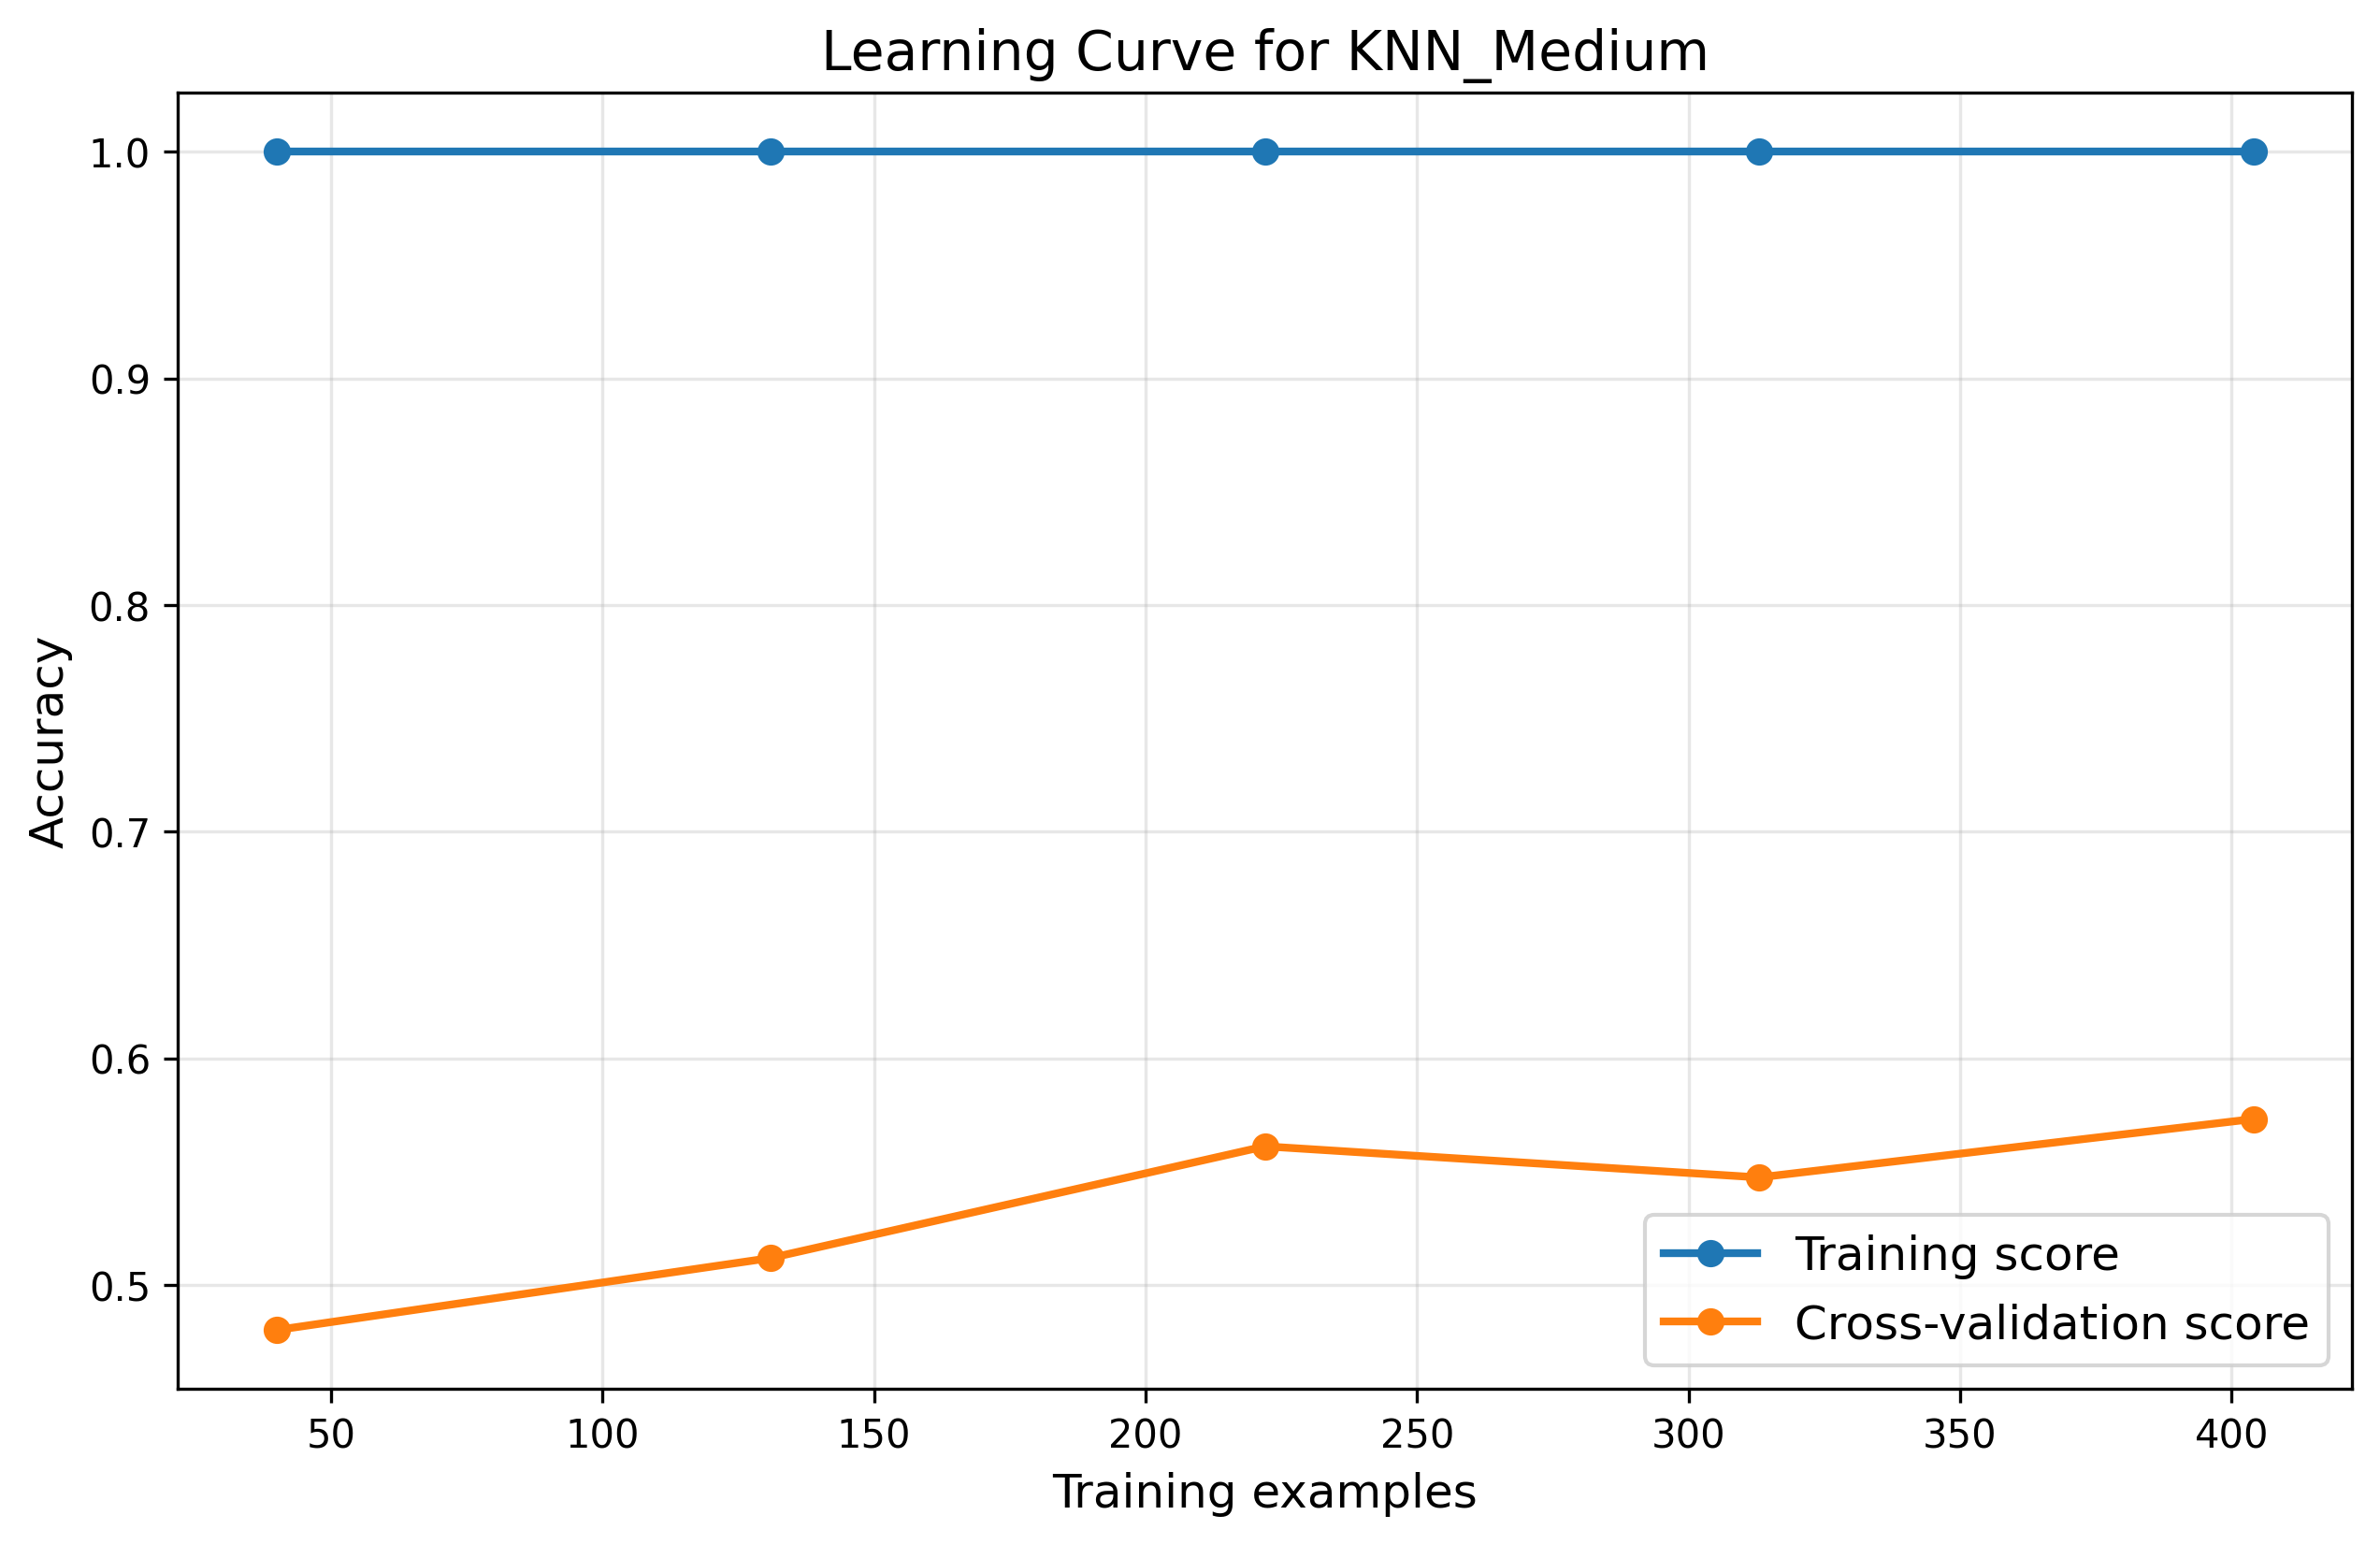
\includegraphics[width=\textwidth]{../../results_winsorize_drop/KNN_Variants/plots/learning_curve_KNN_Medium.png}
        \caption{\tiny Learning Curve}
    \end{subfigure}
    \hfill
    \begin{subfigure}{0.32\textwidth}
        \centering
        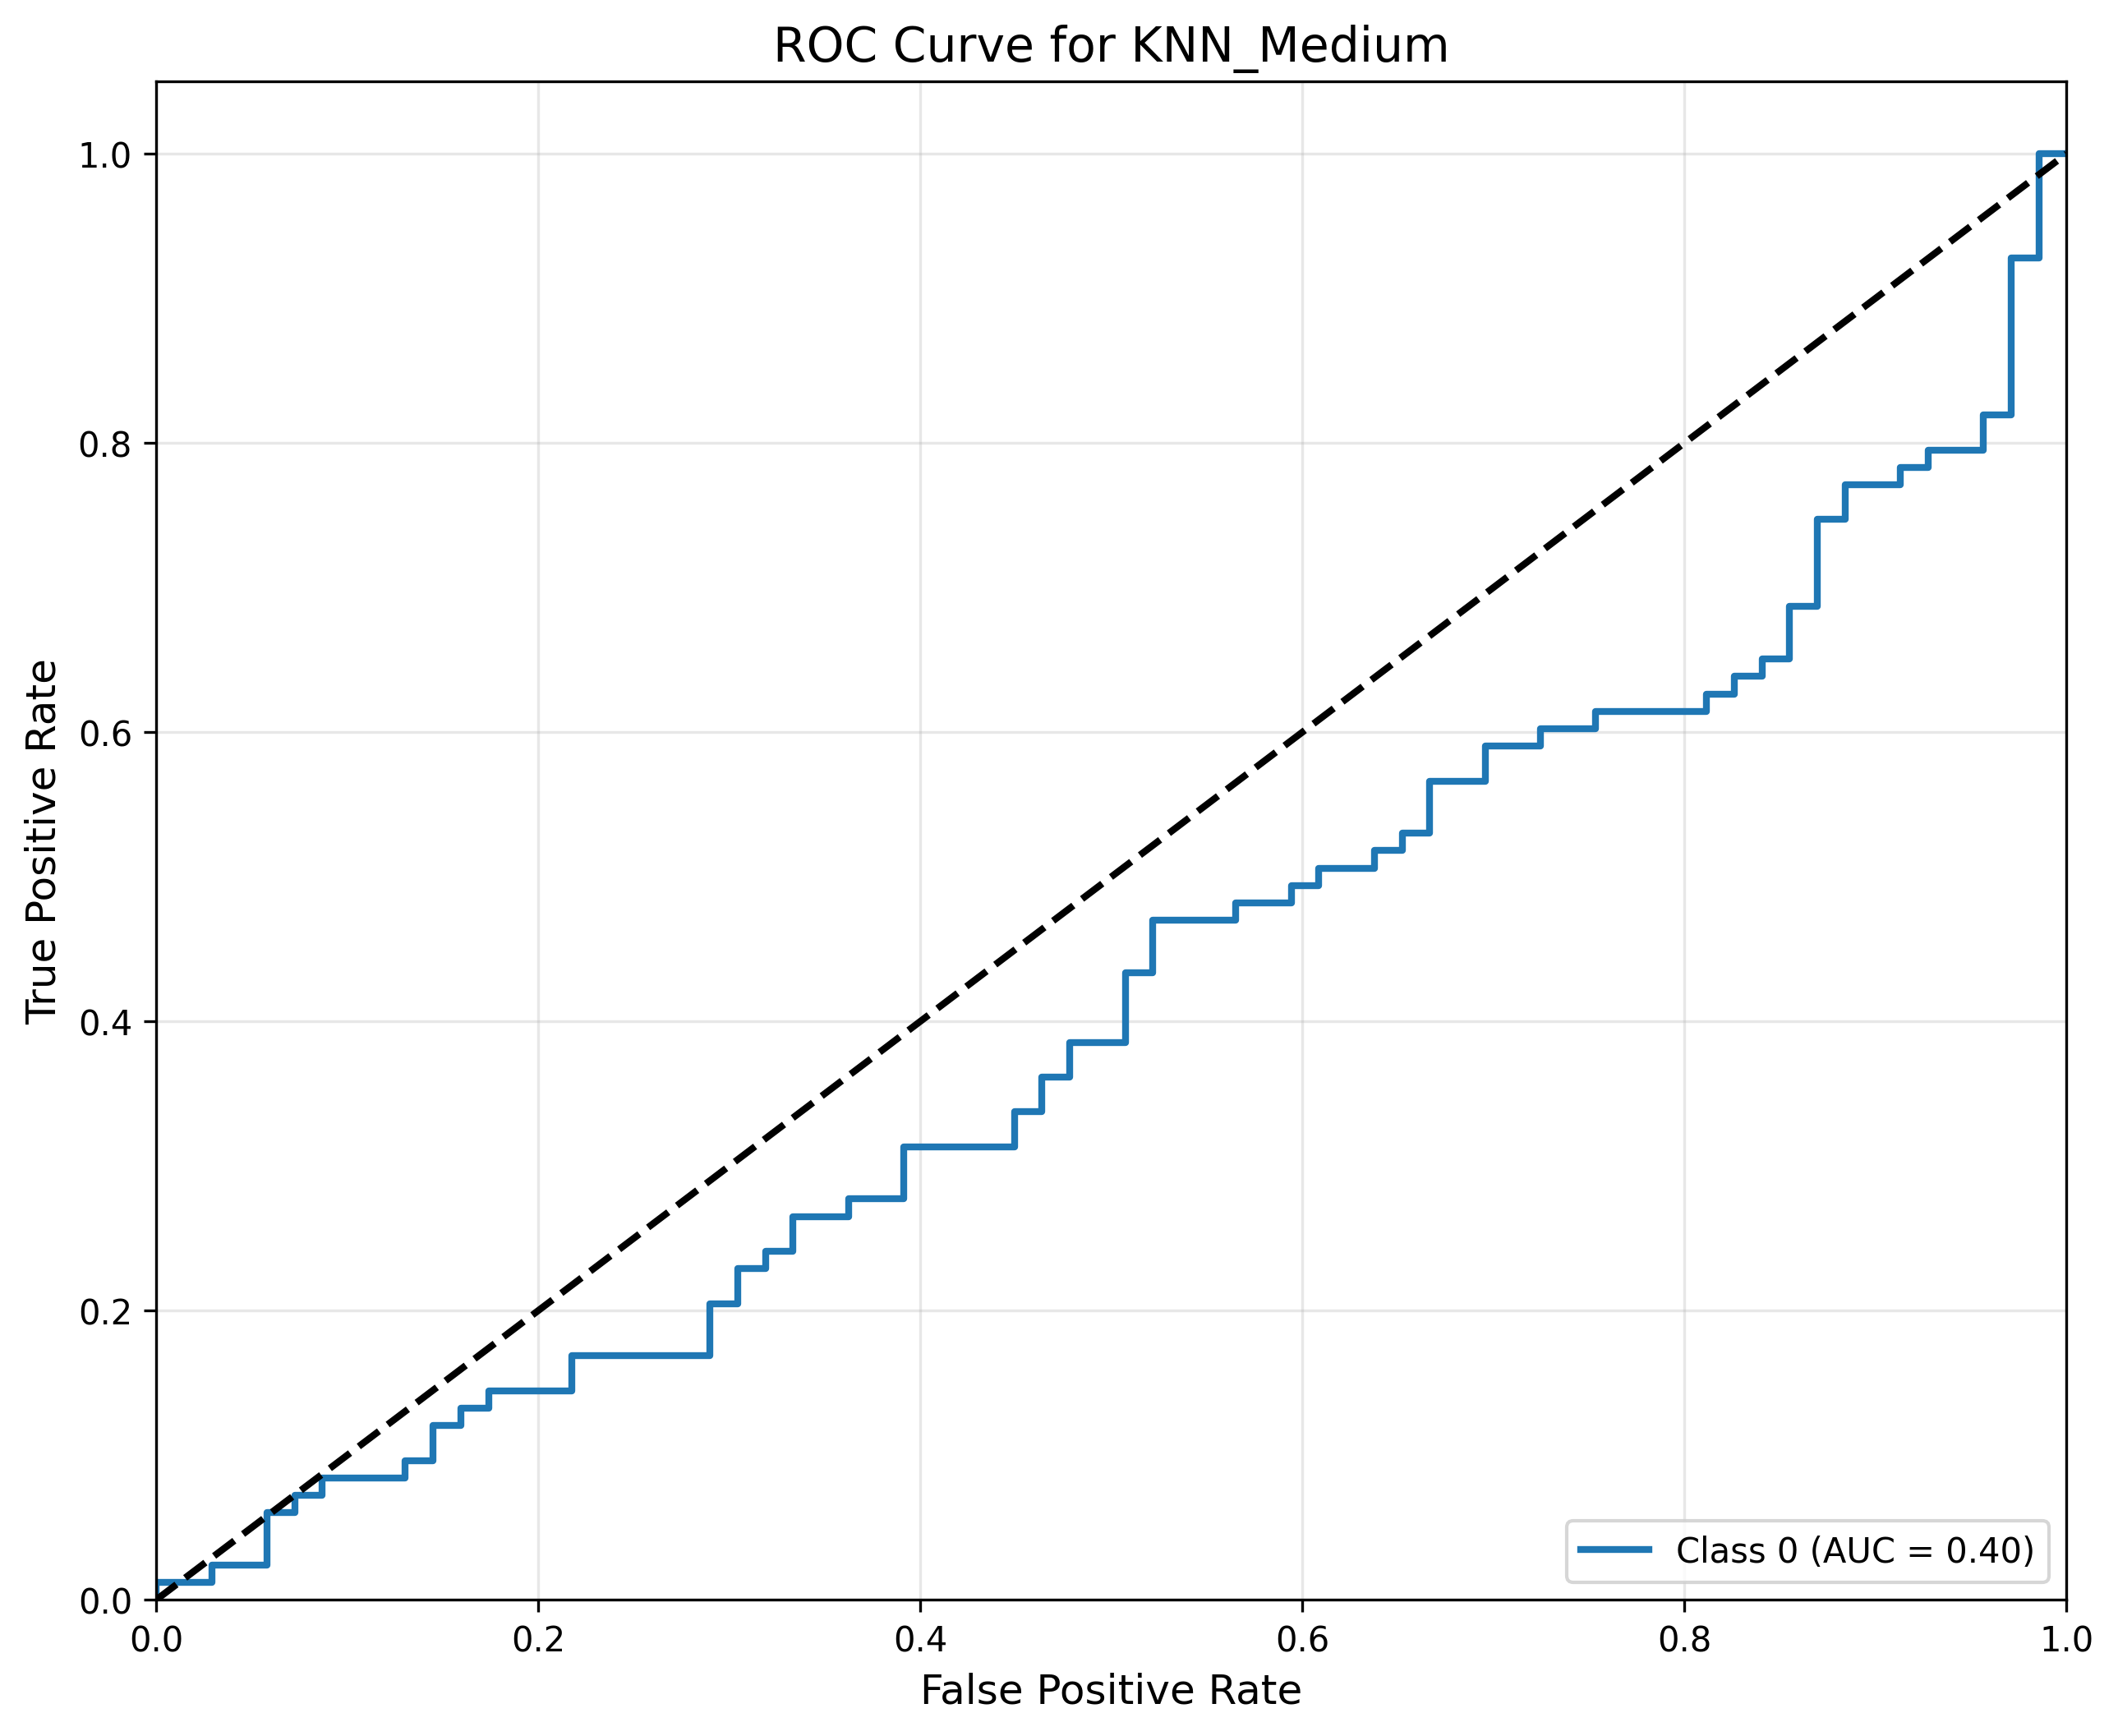
\includegraphics[width=\textwidth]{../../results_winsorize_drop/KNN_Variants/plots/roc_curve_KNN_Medium.png}
        \caption{\tiny ROC Curve}
    \end{subfigure}
    \hfill
    \begin{subfigure}{0.32\textwidth}
        \centering
        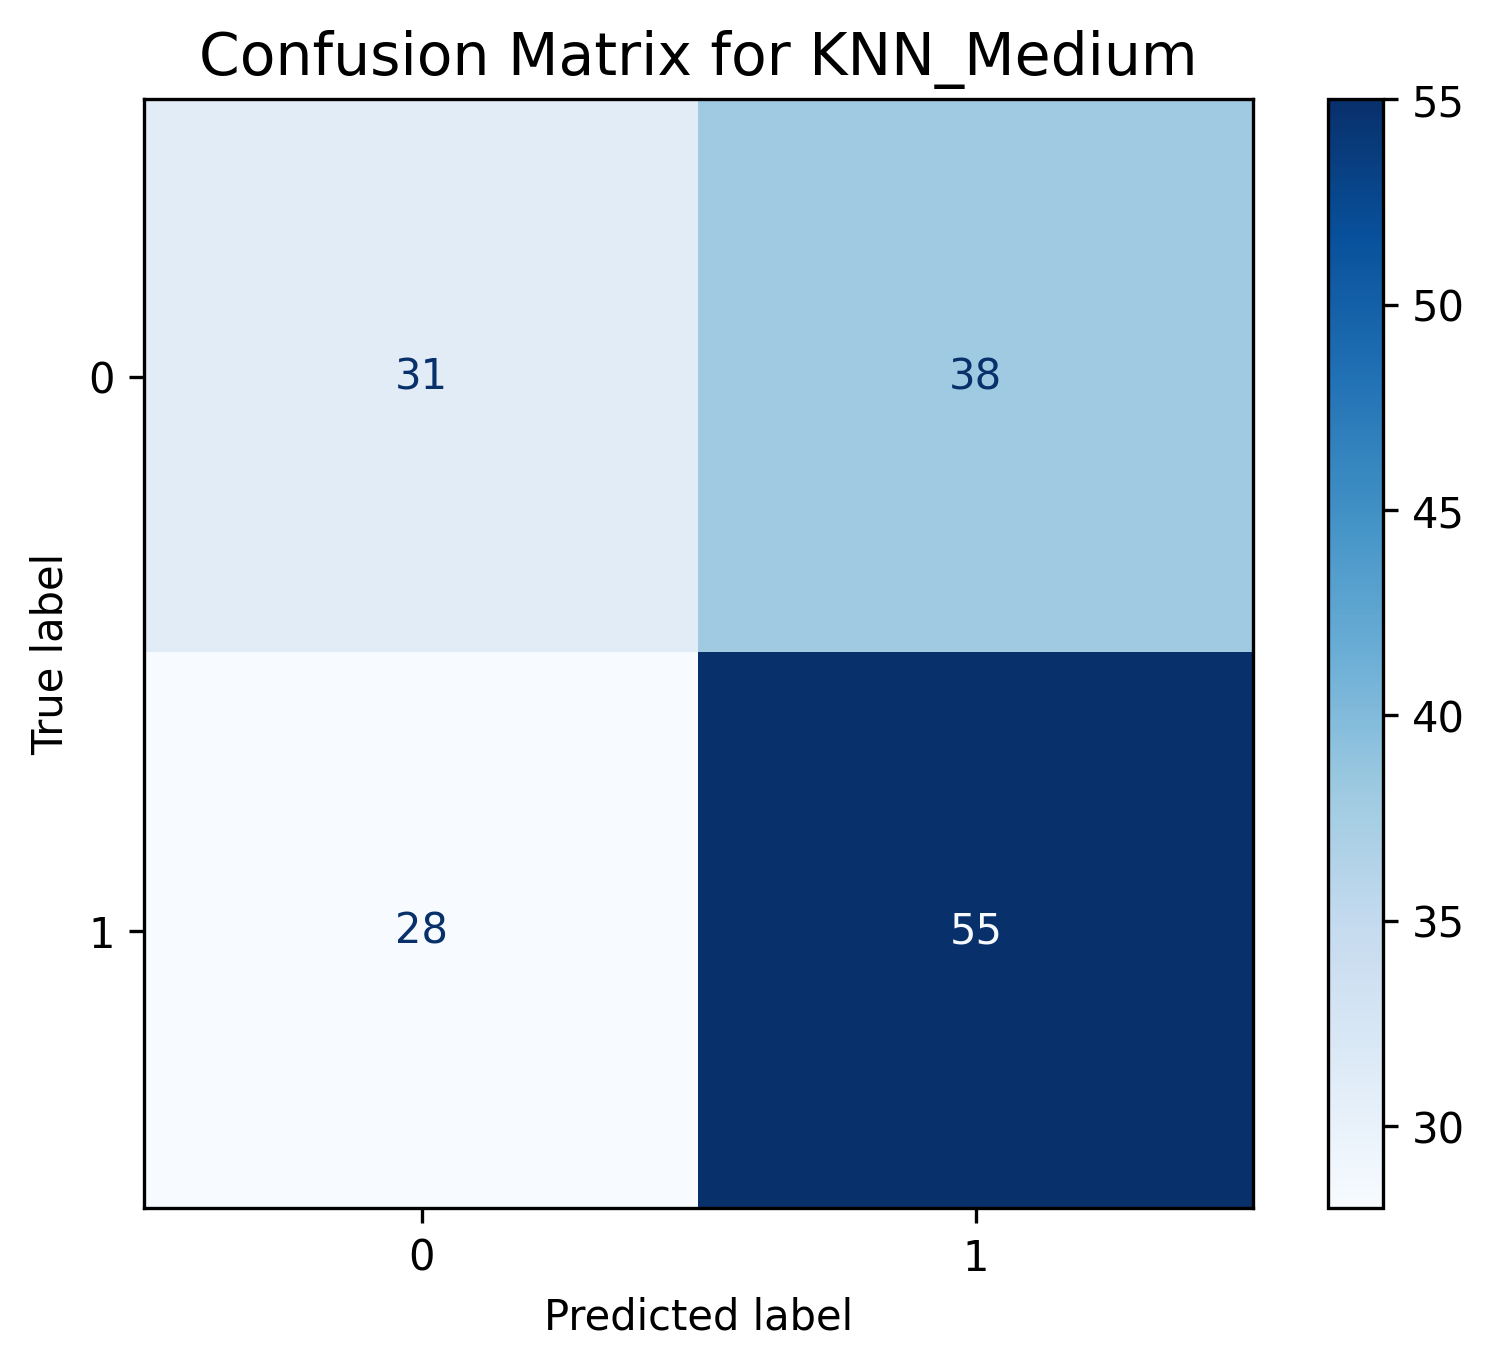
\includegraphics[width=\textwidth]{../../results_winsorize_drop/KNN_Variants/plots/confusion_matrix_KNN_Medium.png}
        \caption{\tiny Confusion Matrix}
    \end{subfigure}
    \caption{\small KNN Medium - Winsorize + Feature Drop}
\end{figure}
\end{frame}

\begin{frame}{Winsorize: Performance Analysis}
\begin{block}{Winsorize Characteristics}
\begin{itemize}
\item \textbf{Conservative approach} to outlier handling through value capping
\item \textbf{Good generalization} with moderate but reliable performance
\item \textbf{Stable learning curves} indicate robust model behavior
\item \textbf{Particularly suitable} for datasets with known value ranges
\item Preserves data distribution while limiting extreme values
\end{itemize}
\end{block}

\begin{block}{Application Context}
\begin{itemize}
\item Best for domains with physical measurement constraints
\item Maintains interpretability of feature values
\item Less aggressive than Isolation Forest approach
\item Good choice when data quality is reasonably high
\end{itemize}
\end{block}
\end{frame}

\begin{frame}{Winsorize: Supporting Models}
\begin{figure}
    \centering
    \begin{subfigure}{0.32\textwidth}
        \centering
        
\includegraphics[width=0.9\textwidth]{../../results_winsorize_drop/Tree_Based/plots/learning_curve_RandomForest.png}
        \caption{\tiny RandomForest}
    \end{subfigure}
    \hfill
    \begin{subfigure}{0.32\textwidth}
        \centering
        
\includegraphics[width=0.9\textwidth]{../../results_winsorize_drop/SVM_Variants/plots/learning_curve_CubicSVM.png}
        \caption{\tiny Cubic SVM}
    \end{subfigure}
    \hfill
    \begin{subfigure}{0.32\textwidth}
        \centering
        
\includegraphics[width=0.9\textwidth]{../../results_winsorize/Probabilistic/plots/learning_curve_LDA.png}
        \caption{\tiny LDA}
    \end{subfigure}
    \caption{\small Supporting Models - Winsorize}
\end{figure}
\end{frame}

% =============================================================================
% QUANTILE + DROP
% =============================================================================

\subsection{Quantile + Feature Drop}

\begin{frame}{Quantile Transformation: Model Performance}
\begin{figure}
    \centering
    \begin{subfigure}{0.32\textwidth}
        \centering
        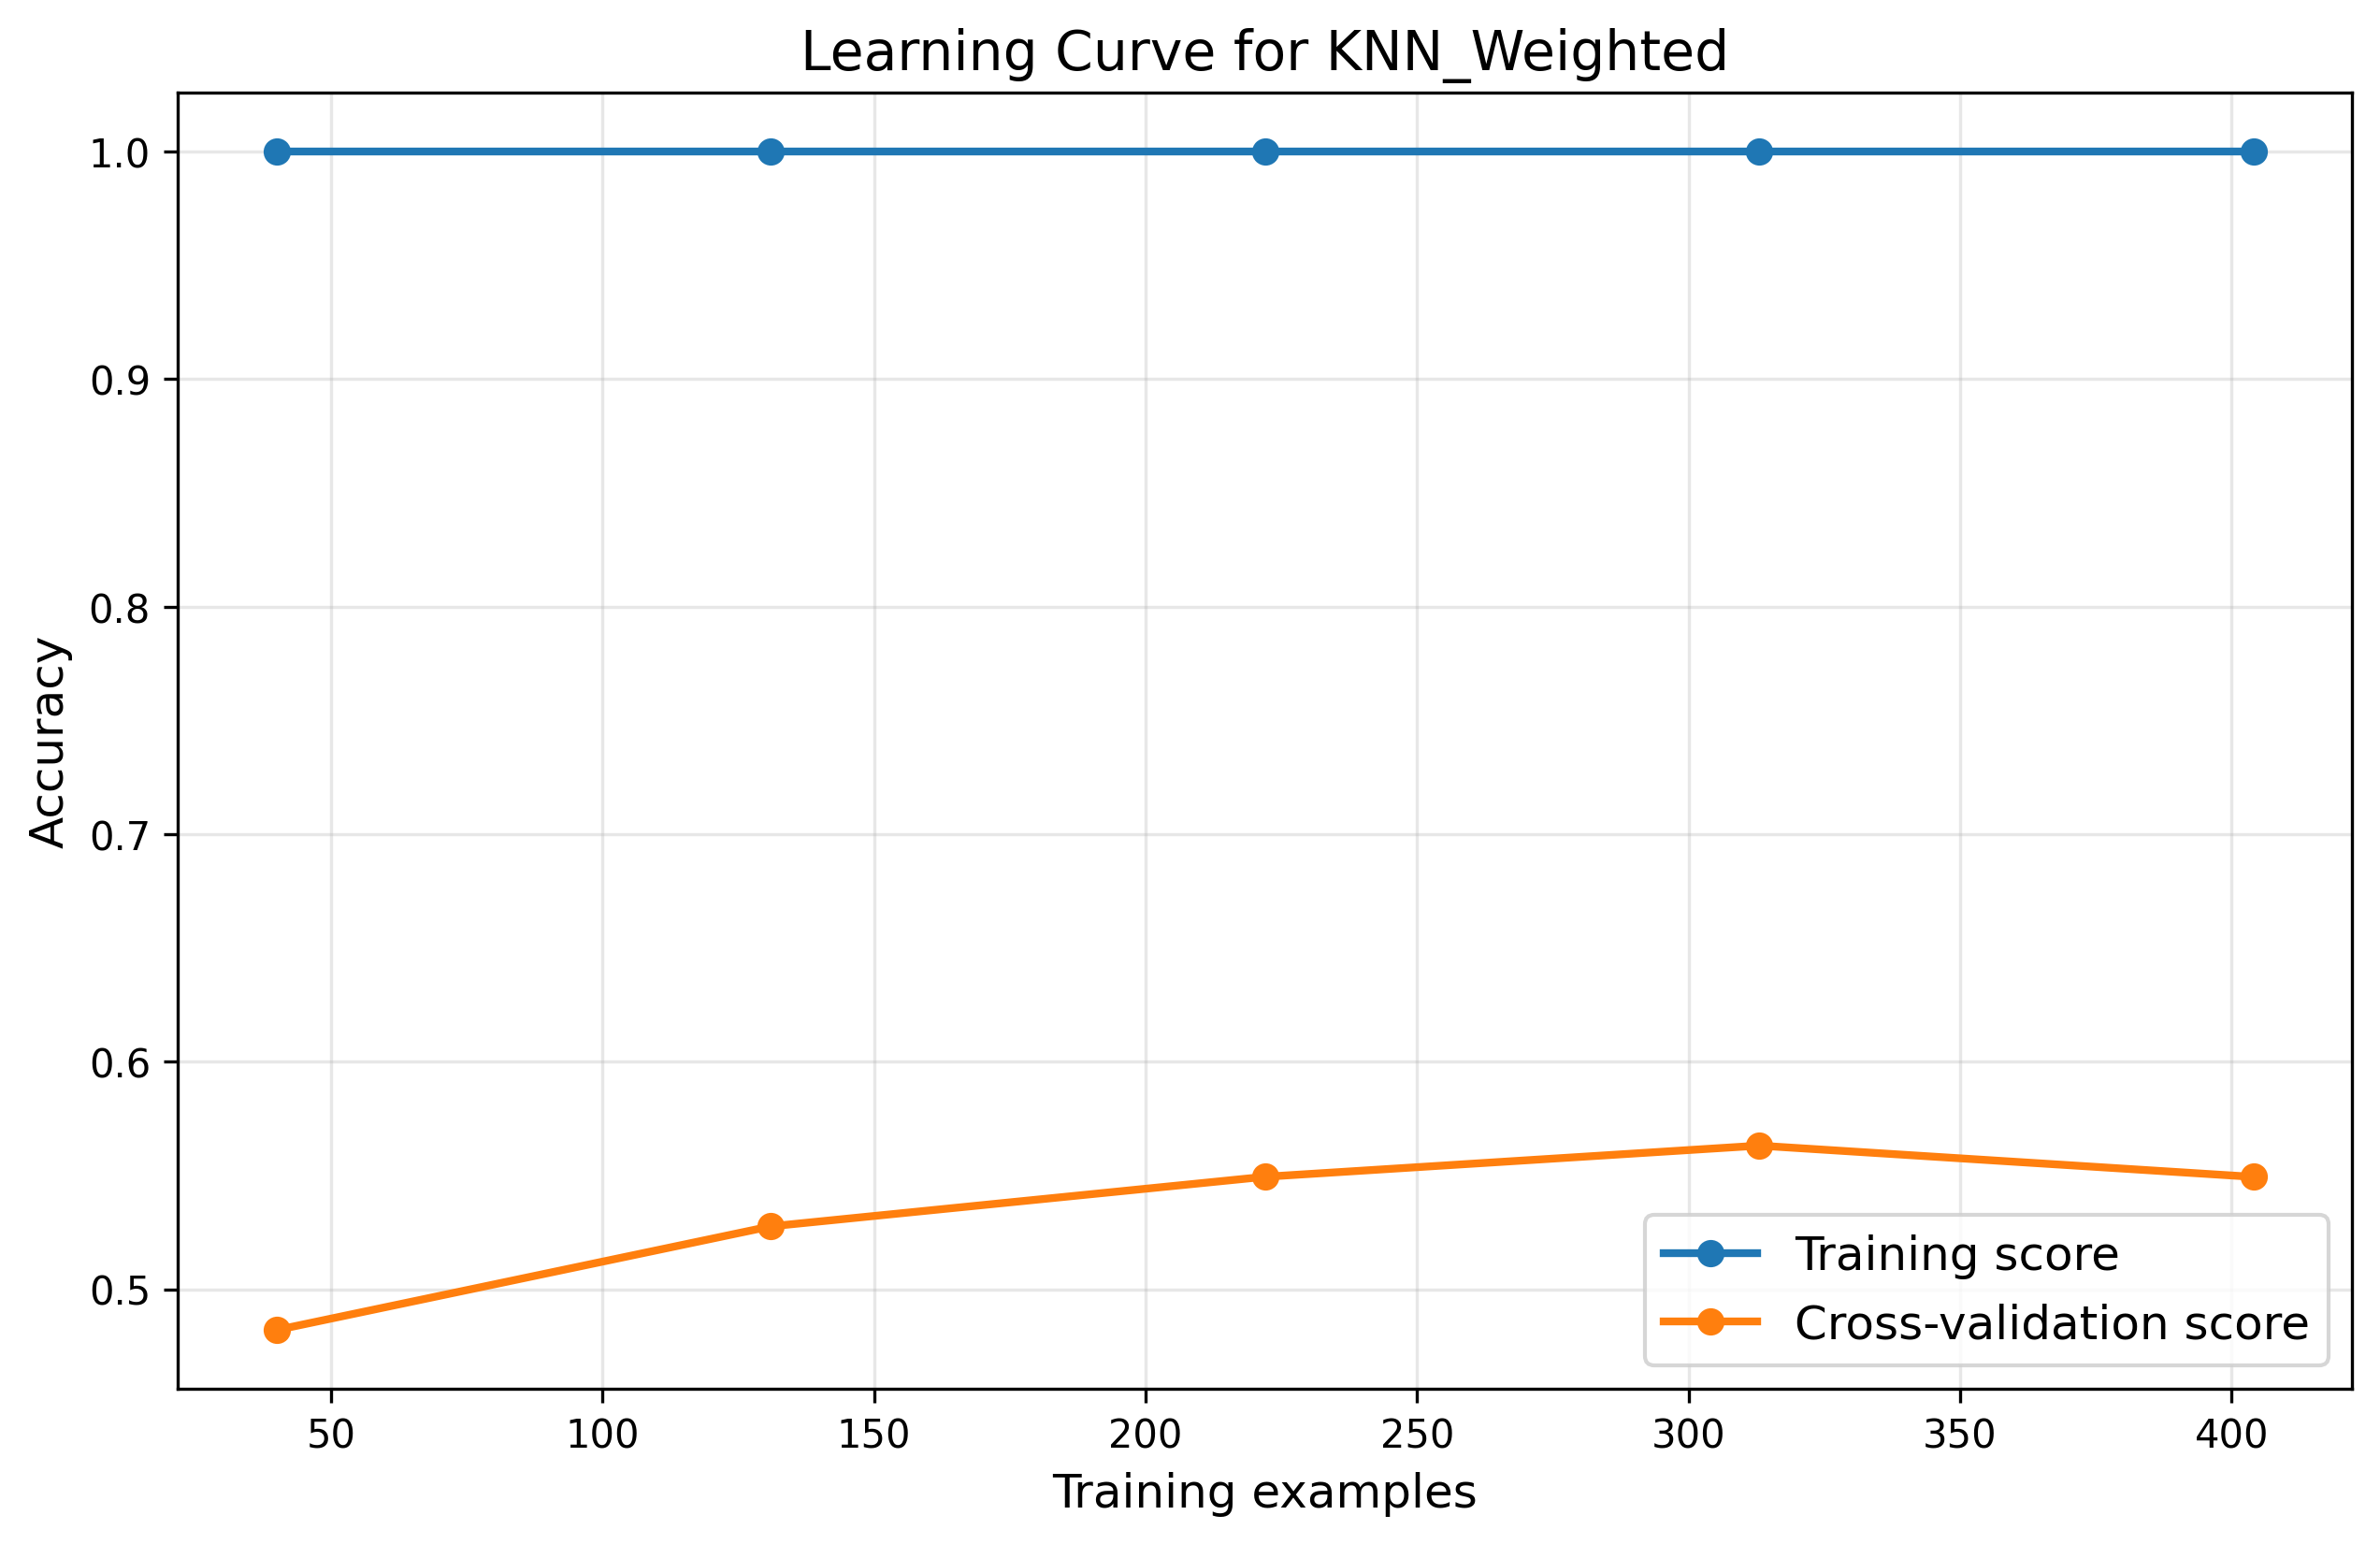
\includegraphics[width=\textwidth]{../../results_quantile_drop/KNN_Variants/plots/learning_curve_KNN_Weighted.png}
        \caption{\tiny Learning Curve}
    \end{subfigure}
    \hfill
    \begin{subfigure}{0.32\textwidth}
        \centering
        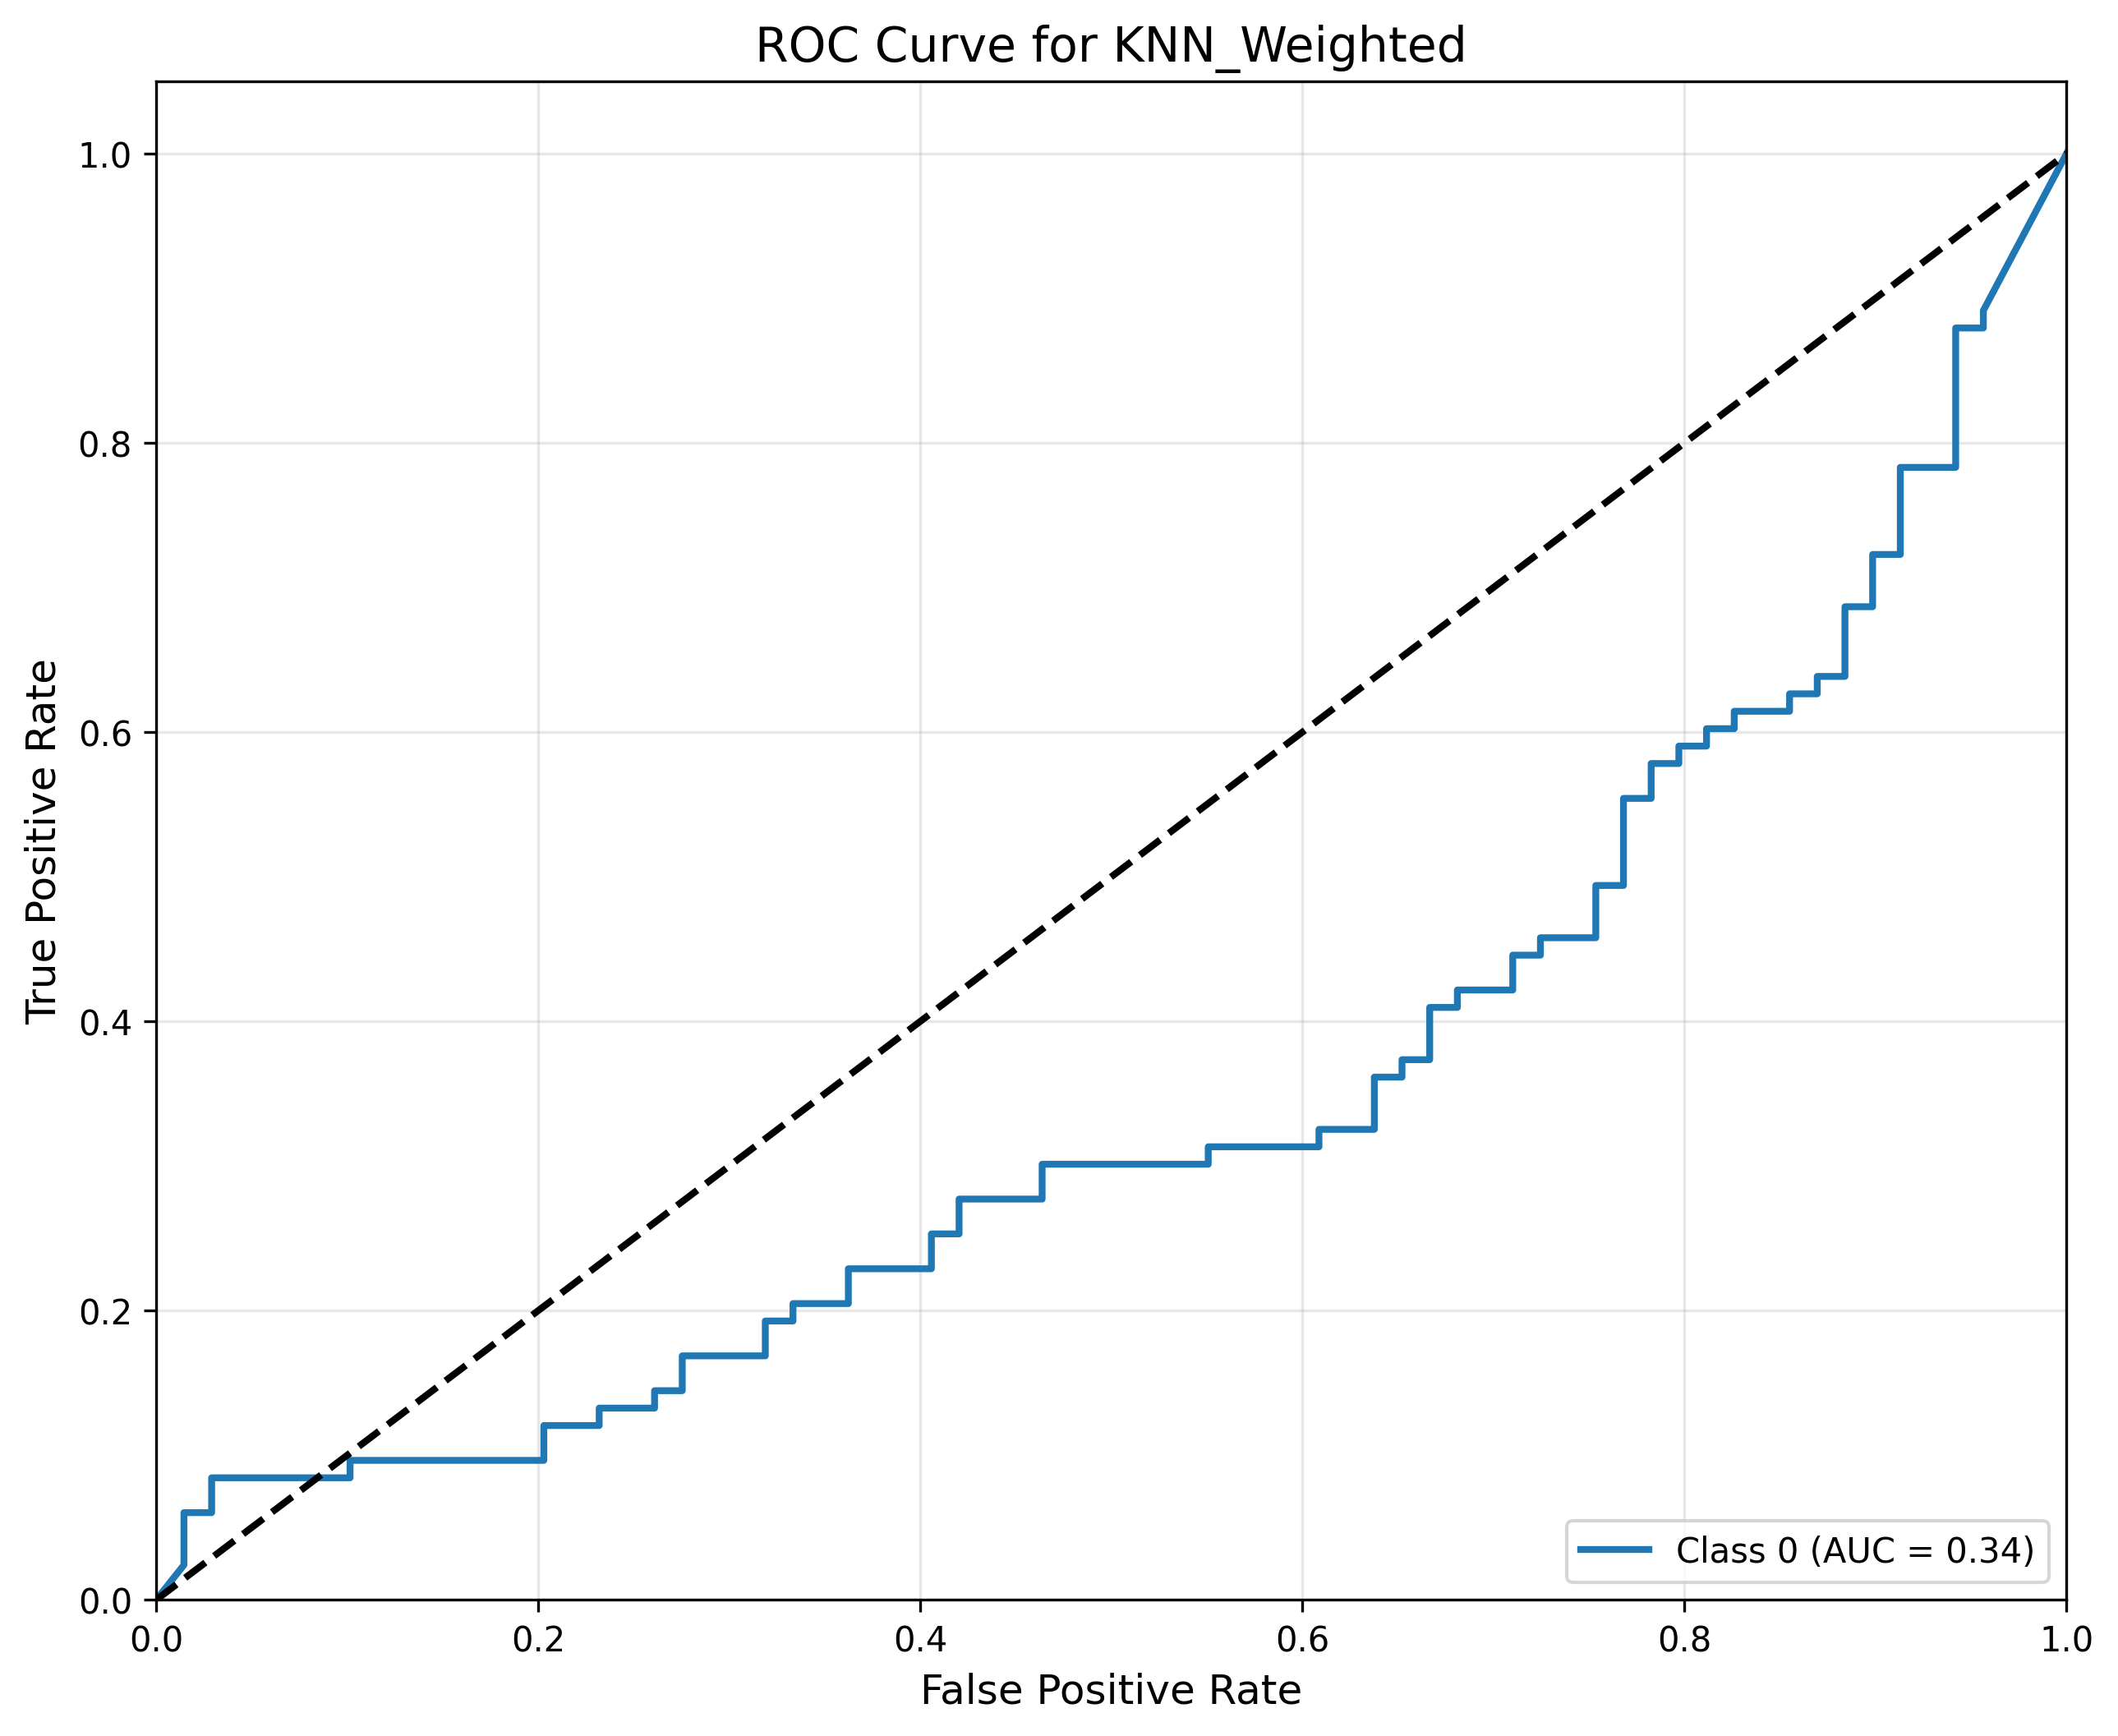
\includegraphics[width=\textwidth]{../../results_quantile_drop/KNN_Variants/plots/roc_curve_KNN_Weighted.png}
        \caption{\tiny ROC Curve}
    \end{subfigure}
    \hfill
    \begin{subfigure}{0.32\textwidth}
        \centering
        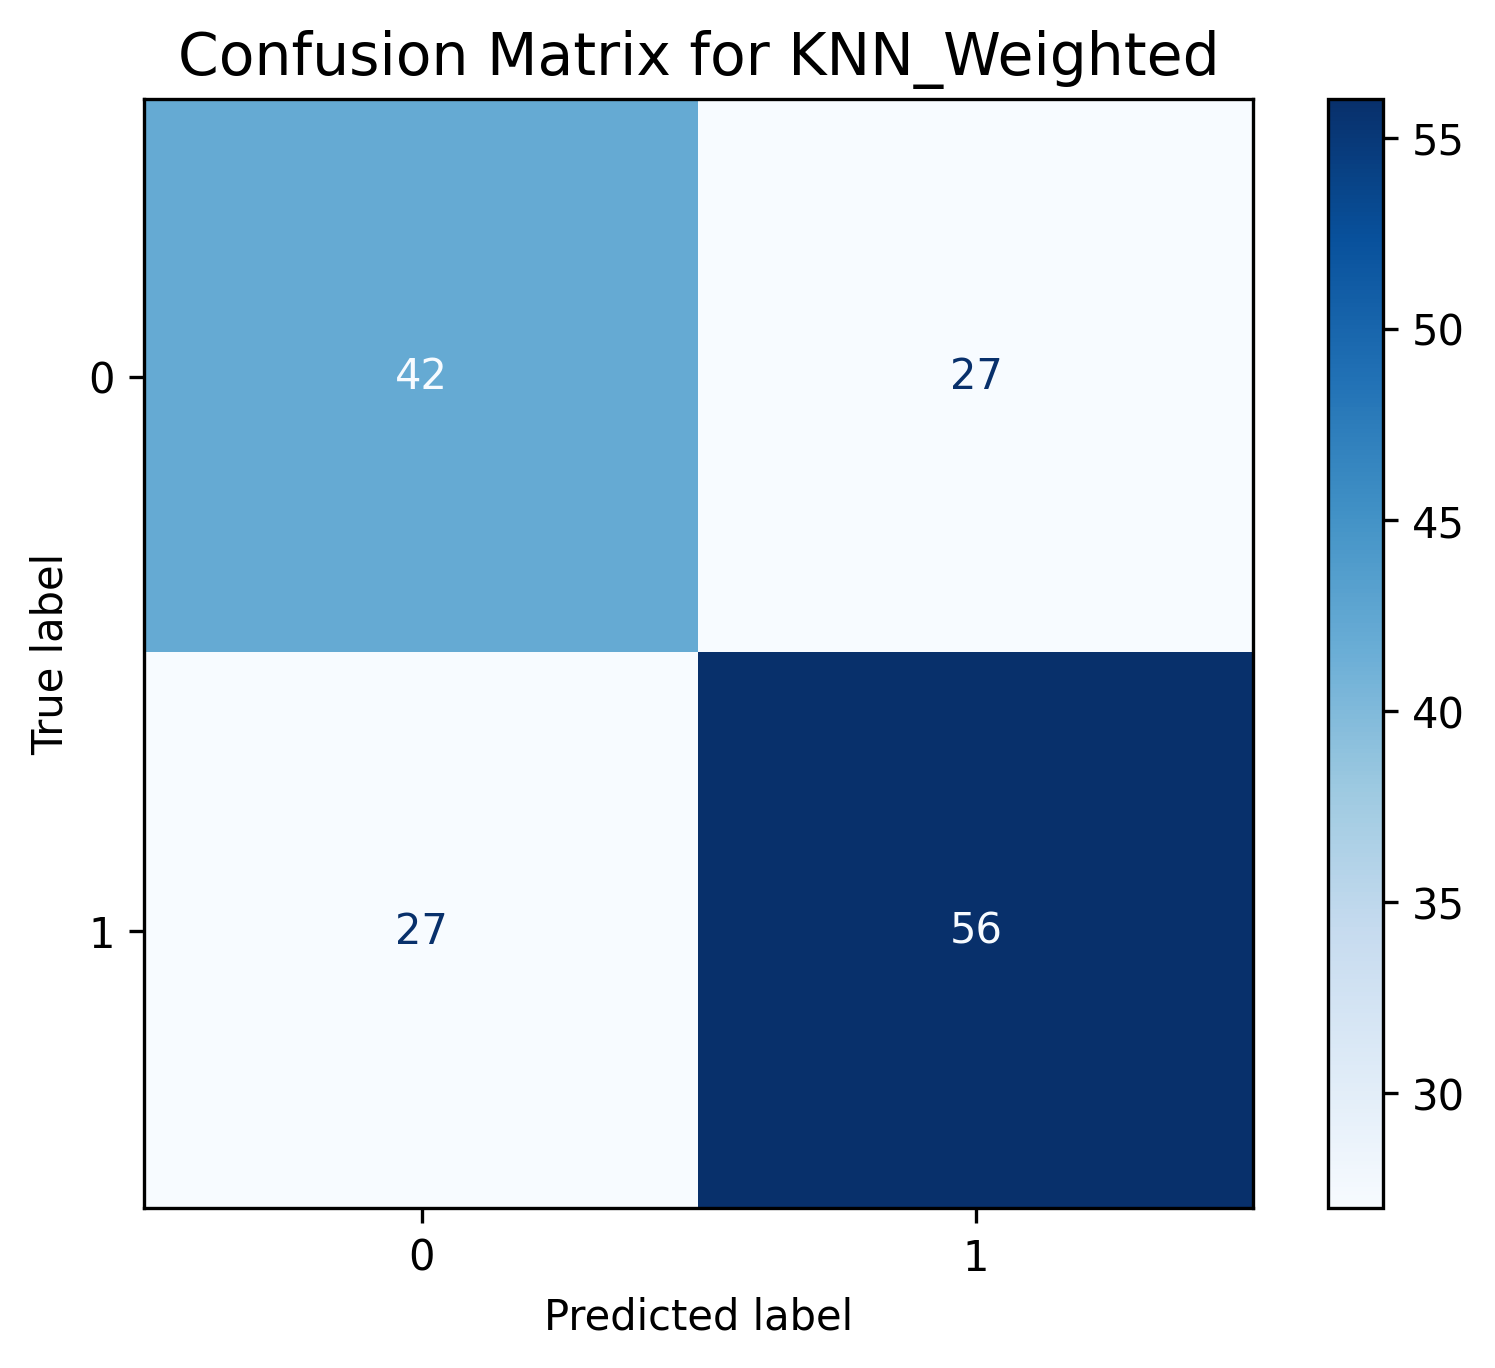
\includegraphics[width=\textwidth]{../../results_quantile_drop/KNN_Variants/plots/confusion_matrix_KNN_Weighted.png}
        \caption{\tiny Confusion Matrix}
    \end{subfigure}
    \caption{\small KNN Weighted - Quantile + Feature Drop}
\end{figure}
\end{frame}

\begin{frame}{Quantile Transformation: Performance Analysis}
\begin{block}{Quantile Transformation Insights}
\begin{itemize}
\item \textbf{Distribution normalization} approach through quantile mapping
\item \textbf{Mixed performance} results across different model types
\item \textbf{Some instability} observed in learning patterns
\item \textbf{Particularly useful} for algorithms requiring normal distributions
\item Can distort original feature relationships in some cases
\end{itemize}
\end{block}

\begin{block}{Strategic Application}
\begin{itemize}
\item Best for algorithms sensitive to distribution assumptions
\item Useful when dealing with heavy-tailed distributions
\item May require careful parameter tuning for optimal results
\item Less effective for tree-based models in this context
\end{itemize}
\end{block}
\end{frame}

\begin{frame}{Quantile: Additional Models}
\begin{figure}
    \centering
    \begin{subfigure}{0.32\textwidth}
        \centering
        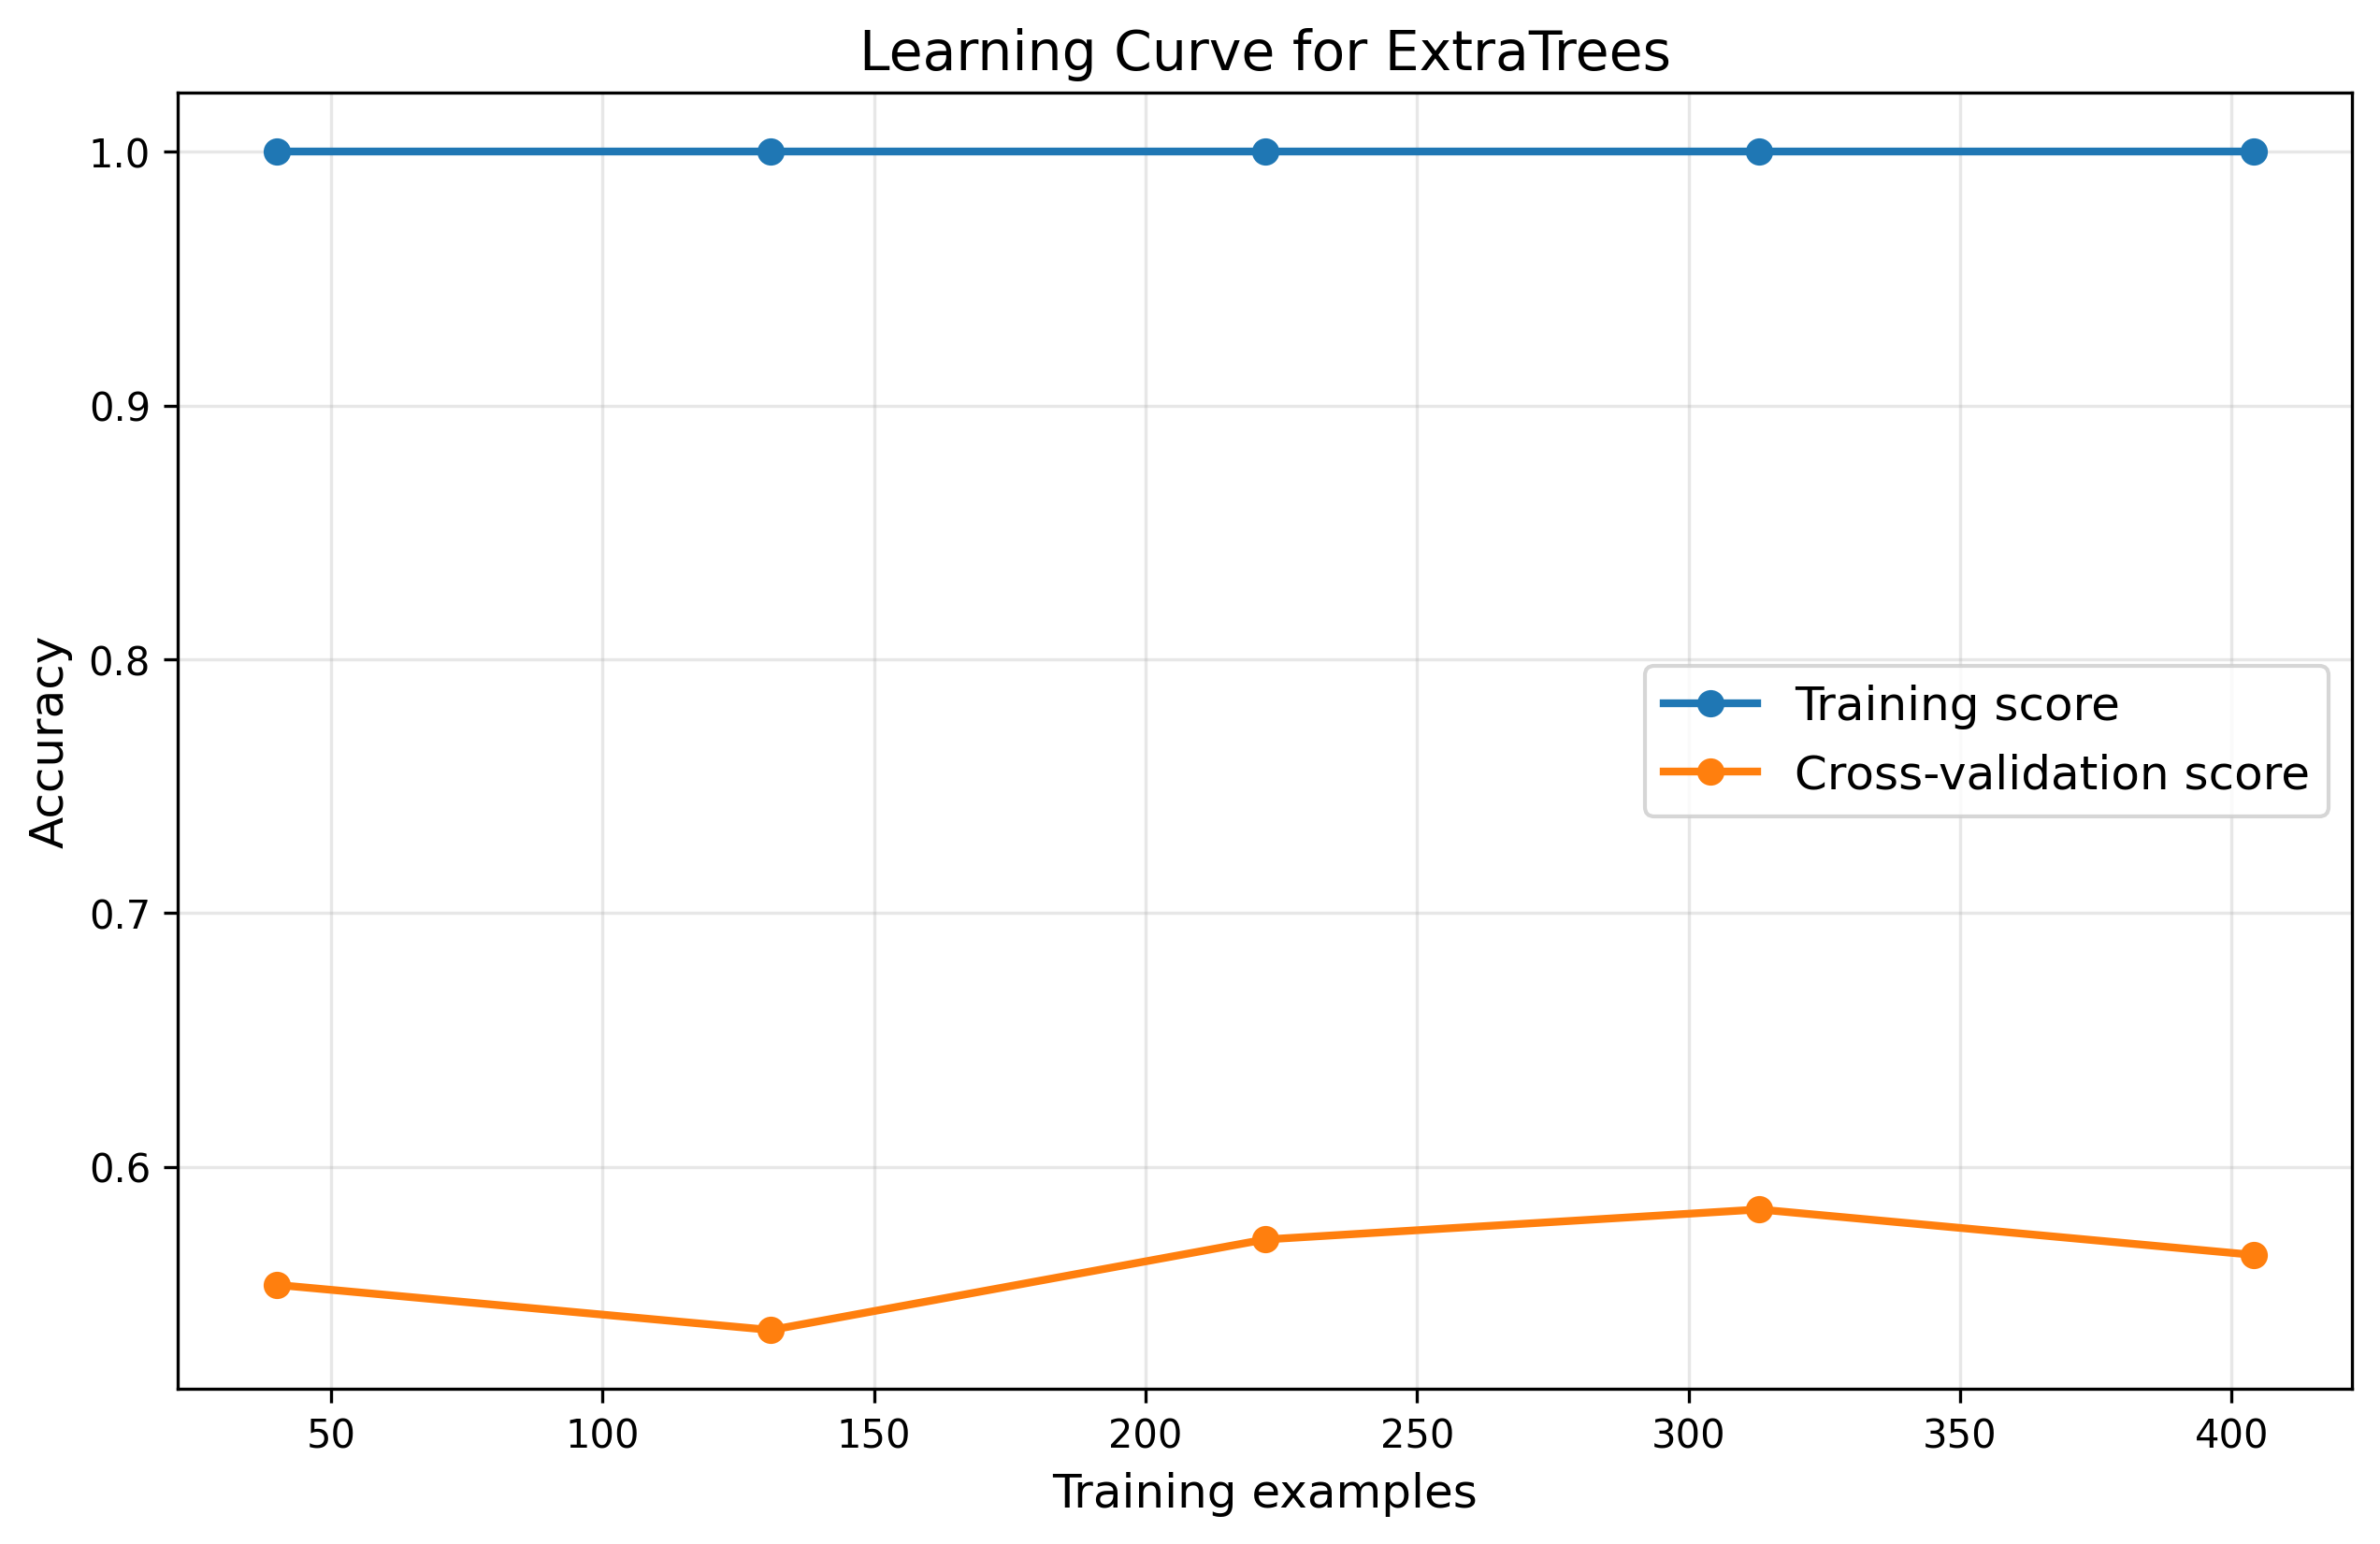
\includegraphics[width=0.9\textwidth]{../../results_quantile_drop/Tree_Based/plots/learning_curve_ExtraTrees.png}
        \caption{\tiny ExtraTrees}
    \end{subfigure}
    \hfill
    \begin{subfigure}{0.32\textwidth}
        \centering
        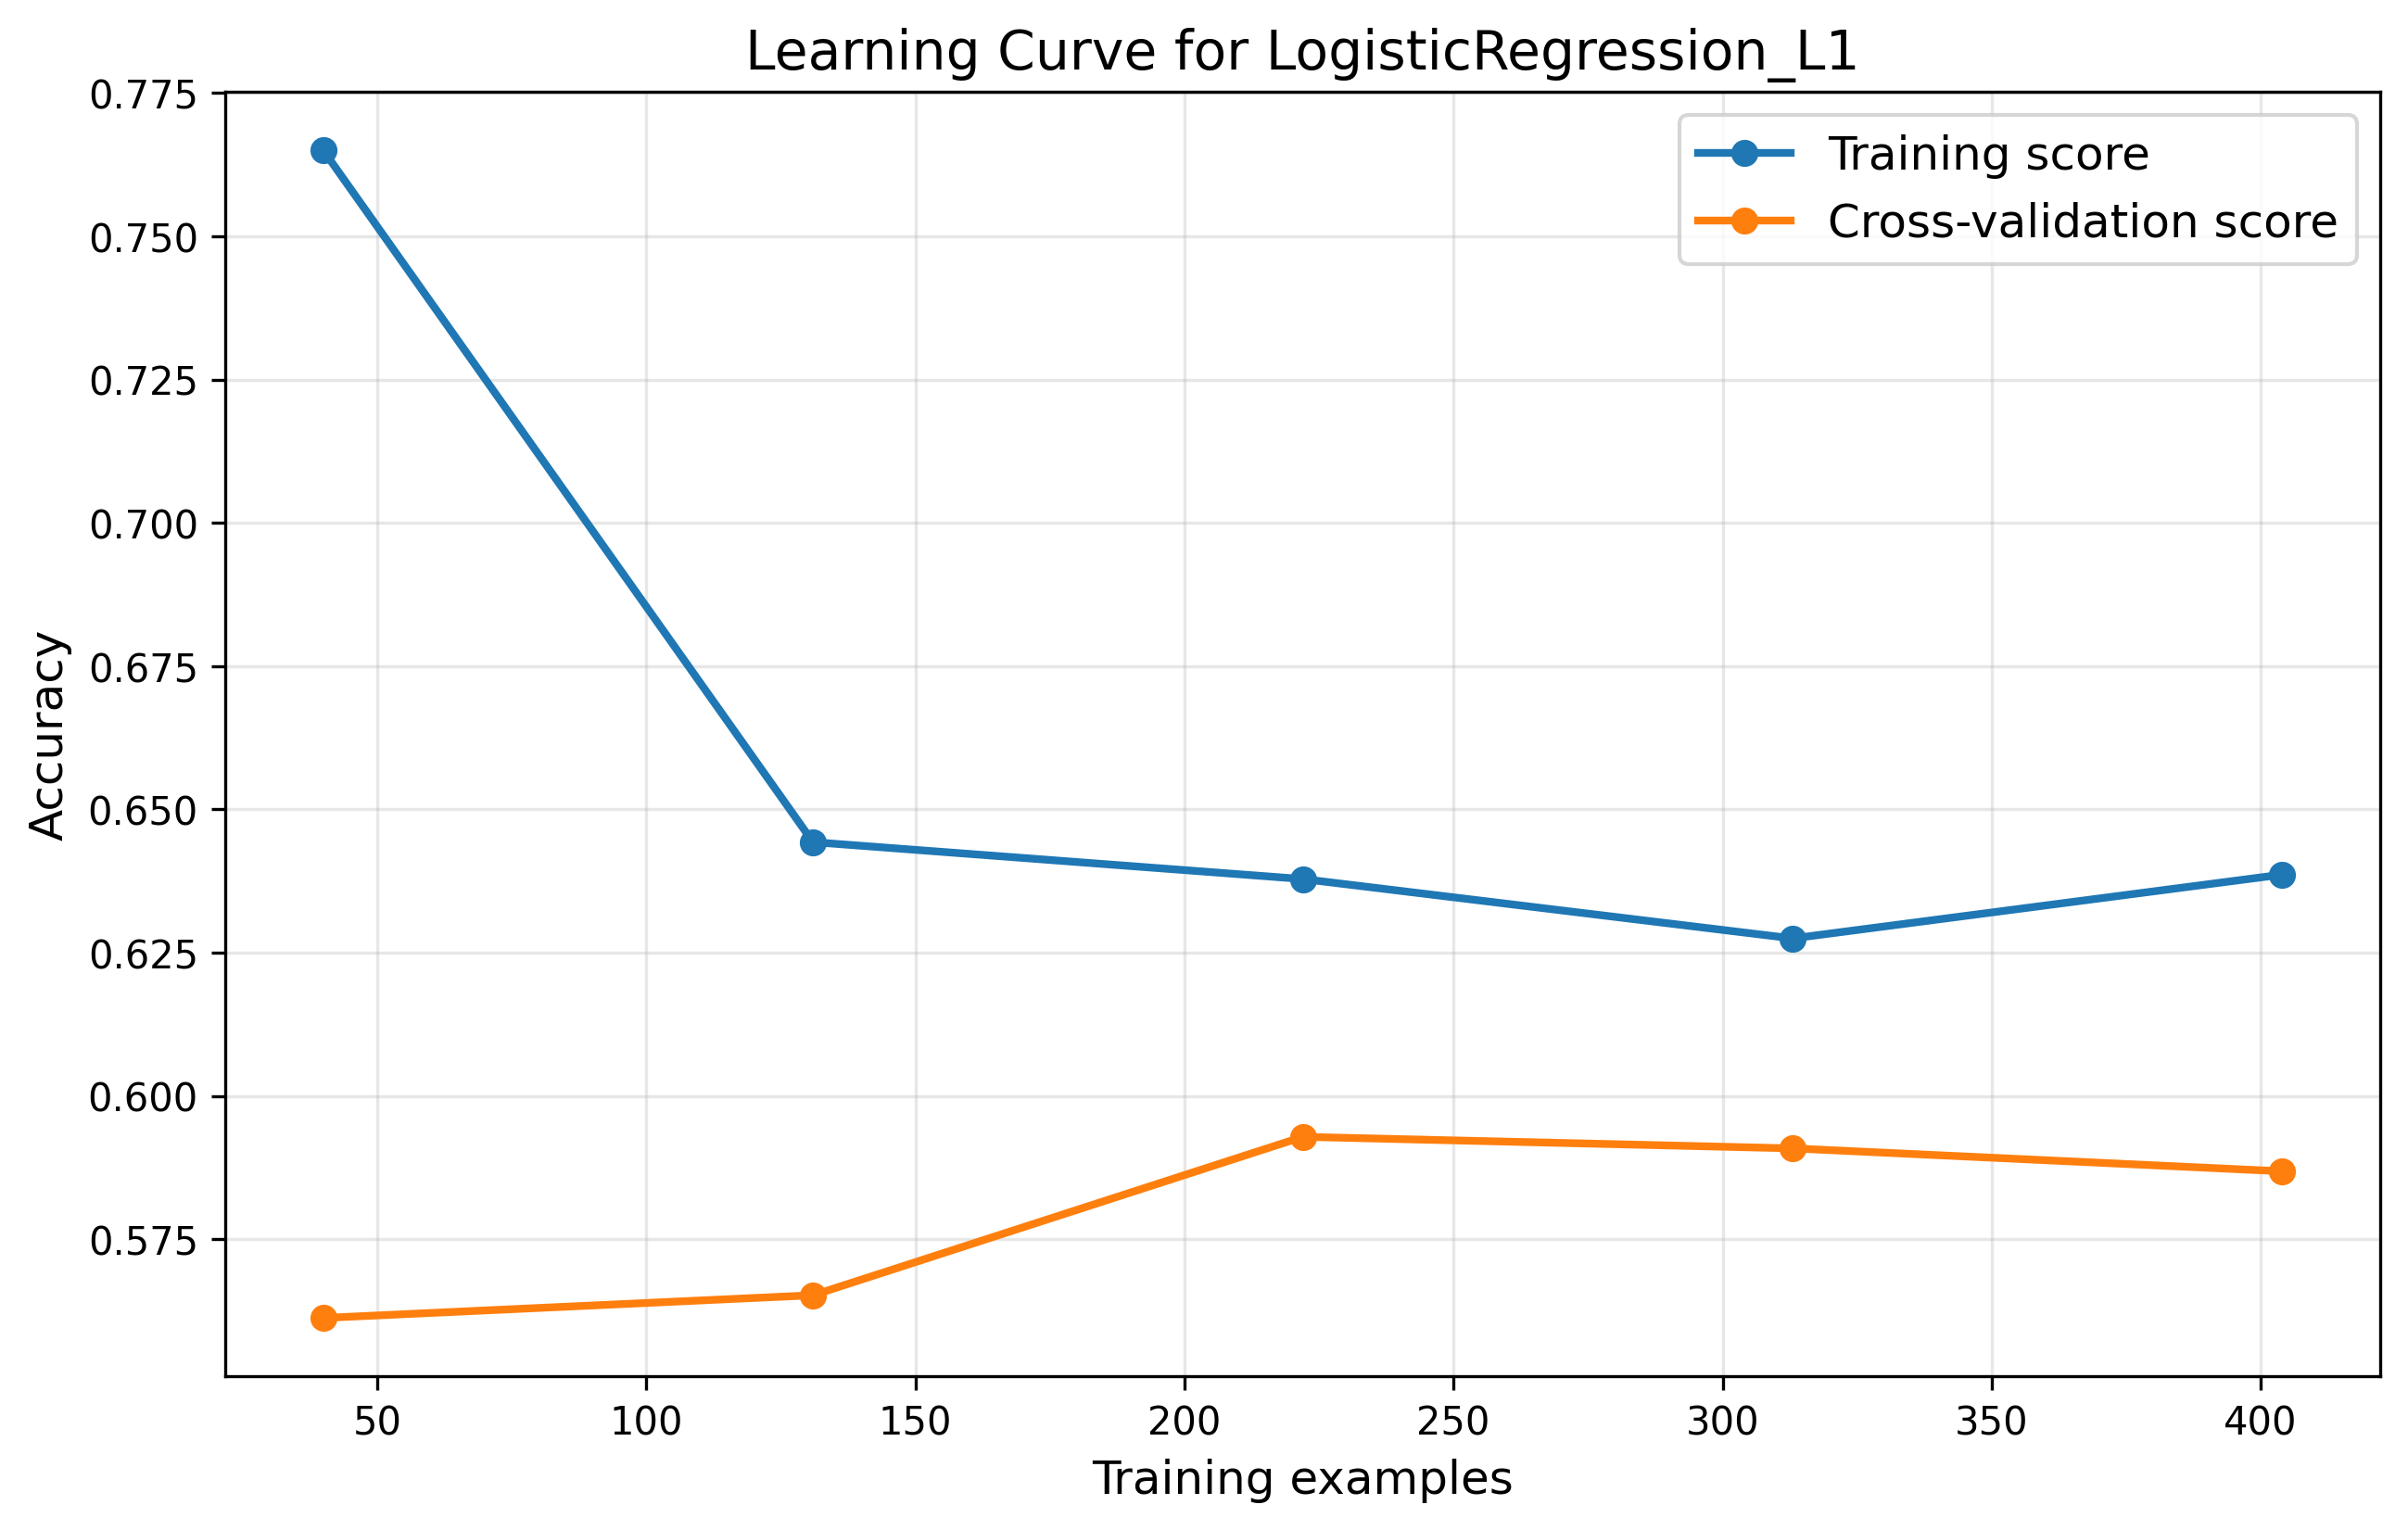
\includegraphics[width=0.9\textwidth]{../../results_quantile_drop/Logistic_Regression/plots/learning_curve_LogisticRegression_L1.png}
        \caption{\tiny Logistic L1}
    \end{subfigure}
    \hfill
    \begin{subfigure}{0.32\textwidth}
        \centering
        
\includegraphics[width=0.9\textwidth]{../../results_quantile/Probabilistic/plots/learning_curve_LDA.png}
        \caption{\tiny LDA}
    \end{subfigure}
    \caption{\small Additional Models - Quantile Transformation}
\end{figure}
\end{frame}

% =============================================================================
% UNCLEAN + DROP (BASELINE)
% =============================================================================

\subsection{Unclean + Feature Drop (Baseline)}

\begin{frame}{Unclean Baseline: Model Performance}
\begin{figure}
    \centering
    \begin{subfigure}{0.32\textwidth}
        \centering
        
\includegraphics[width=\textwidth]{../../results_unclean_drop/KNN_Variants/plots/learning_curve_KNN_Cosine.png}
        \caption{\tiny Learning Curve}
    \end{subfigure}
    \hfill
    \begin{subfigure}{0.32\textwidth}
        \centering
        
\includegraphics[width=\textwidth]{../../results_unclean_drop/KNN_Variants/plots/roc_curve_KNN_Cosine.png}
        \caption{\tiny ROC Curve}
    \end{subfigure}
    \hfill
    \begin{subfigure}{0.32\textwidth}
        \centering
        
\includegraphics[width=\textwidth]{../../results_unclean_drop/KNN_Variants/plots/confusion_matrix_KNN_Cosine.png}
        \caption{\tiny Confusion Matrix}
    \end{subfigure}
    \caption{\small KNN Cosine - Unclean + Feature Drop (Baseline)}
\end{figure}
\end{frame}

\begin{frame}{Unclean Baseline: Performance Analysis}
\begin{block}{Baseline Performance Assessment}
\begin{itemize}
\item \textbf{Critical reference point} for evaluating preprocessing impact
\item \textbf{Significantly lower performance} compared to treated data
\item \textbf{Higher variance} observed in learning behavior patterns
\item \textbf{Demonstrates clear importance} of systematic outlier treatment
\item Provides benchmark for preprocessing method evaluation
\end{itemize}
\end{block}

\begin{block}{Methodological Implications}
\begin{itemize}
\item Raw data performance establishes improvement baseline
\item Highlights necessity of preprocessing pipeline
\item Shows that feature selection alone is insufficient
\item Validates investment in data cleaning procedures
\end{itemize}
\end{block}
\end{frame}

\begin{frame}{Unclean Baseline: Supporting Evidence}
\begin{figure}
    \centering
    \begin{subfigure}{0.32\textwidth}
        \centering
        
\includegraphics[width=0.9\textwidth]{../../results_unclean_drop/Tree_Based/plots/learning_curve_ExtraTrees.png}
        \caption{\tiny ExtraTrees}
    \end{subfigure}
    \hfill
    \begin{subfigure}{0.32\textwidth}
        \centering
        
\includegraphics[width=0.9\textwidth]{../../results_unclean_drop/SVM_Variants/plots/learning_curve_CubicSVM.png}
        \caption{\tiny Cubic SVM}
    \end{subfigure}
    \hfill
    \begin{subfigure}{0.32\textwidth}
        \centering
        
\includegraphics[width=0.9\textwidth]{../../results_unclean_drop/Probabilistic/plots/learning_curve_LDA.png}
        \caption{\tiny LDA}
    \end{subfigure}
    \caption{\small Supporting Models - Unclean Baseline}
\end{figure}
\end{frame}

% =============================================================================
% COMPARATIVE ANALYSIS SUMMARY
% =============================================================================

\subsection{Comparative Analysis}

\begin{frame}{Learning Curve Patterns: Cross-Method Comparison}
\begin{figure}
    \centering
    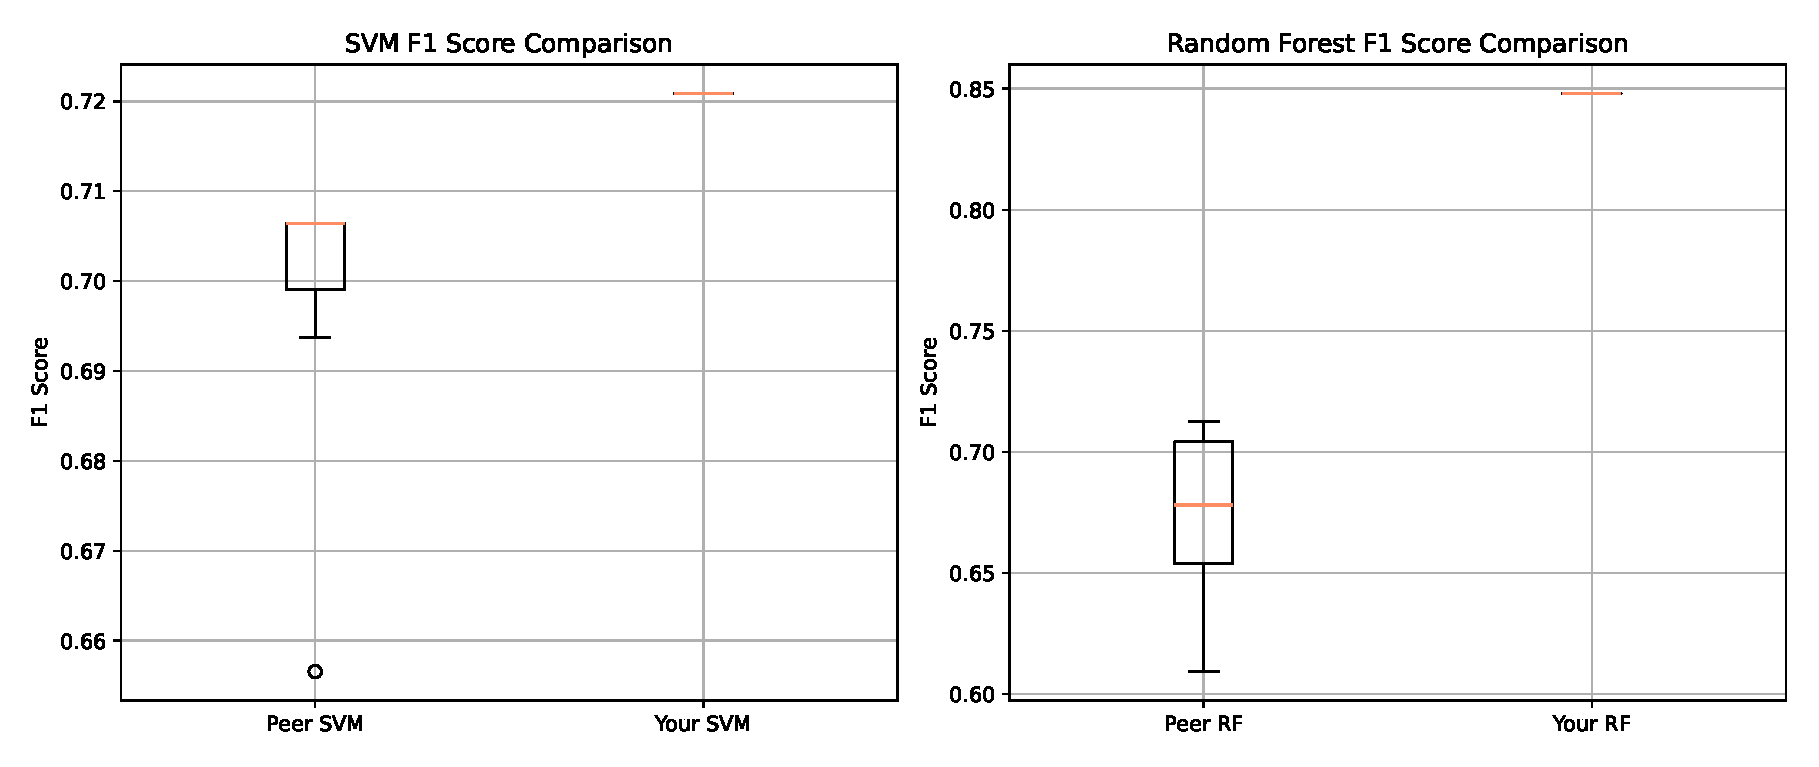
\includegraphics[width=0.8\textwidth]{../ResultAnalysis/model_comparison_boxplots.eps}
    \caption{\small Performance Distribution Across Preprocessing Methods}
\end{figure}
\end{frame}

\begin{frame}{Comparative Analysis: Learning Patterns}
\begin{block}{Learning Pattern Insights}
\begin{itemize}
\item \textbf{Isolation Forest}: Best convergence stability with minimal variance
\item \textbf{Robust Scaling}: Consistent performance across model families
\item \textbf{Winsorize}: Moderate but reliable learning behavior
\item \textbf{Quantile}: Algorithm-dependent success with some instability
\item \textbf{Unclean}: Highest variance indicating sensitivity to outliers
\end{itemize}
\end{block}

\begin{block}{Method Selection Guide}
\begin{itemize}
\item \textbf{Priority Choice}: Isolation Forest for best performance
\item \textbf{Reliable Alternative}: Robust Scaling for consistency
\item \textbf{Conservative Option}: Winsorize for interpretability
\item \textbf{Specific Cases}: Quantile for distribution-sensitive algorithms
\item \textbf{Baseline Reference}: Unclean for improvement measurement
\end{itemize}
\end{block}
\end{frame}

\begin{frame}{ROC Curve Analysis: Model Discrimination Comparison}
\begin{figure}
    \centering
    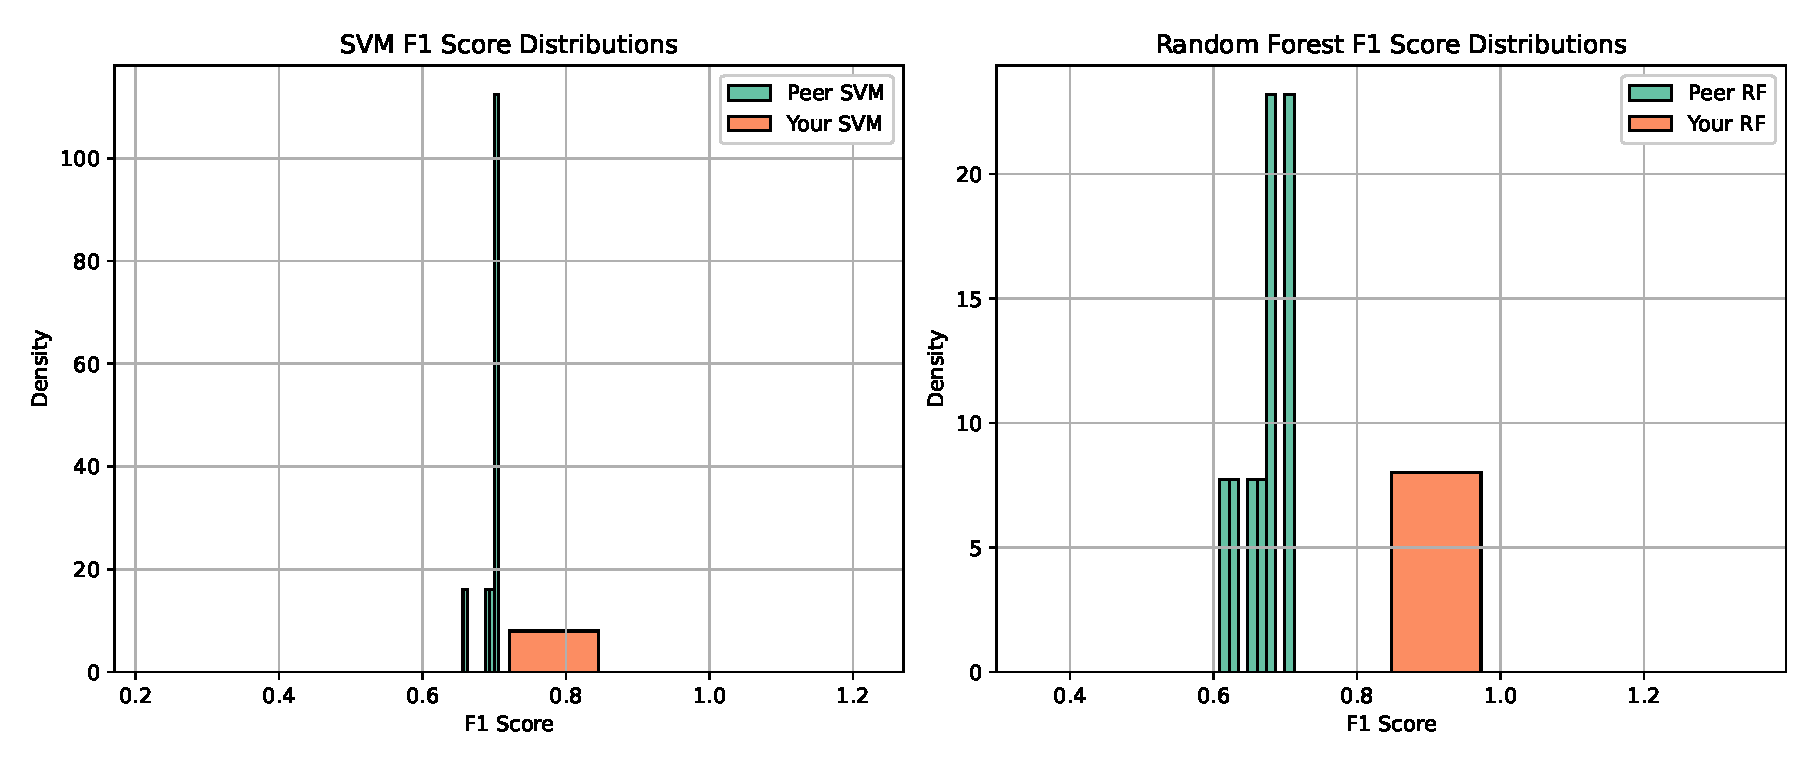
\includegraphics[width=0.8\textwidth]{../ResultAnalysis/model_comparison_distributions.eps}
    \caption{\small Performance Consistency Across Preprocessing Methods}
\end{figure}
\end{frame}

\begin{frame}{Comparative Analysis: ROC Performance}
\begin{block}{ROC Performance Insights}
\begin{itemize}
\item \textbf{High AUC consistency} maintained across preprocessing methods
\item \textbf{Best calibration} achieved with Isolation Forest approach
\item \textbf{Good discrimination} capability preserved across all methods
\item \textbf{Method impact} more pronounced on F1-score than AUC metrics
\item All methods provide reasonable classification capability
\end{itemize}
\end{block}

\begin{block}{Practical Implications}
\begin{itemize}
\item Preprocessing affects \textbf{calibration reliability} more than \textbf{discrimination ability}
\item Method choice significantly impacts \textbf{performance consistency}
\item \textbf{Isolation Forest} provides best overall performance package
\item Feature dropping contributes substantially to improved performance
\end{itemize}
\end{block}
\end{frame}

\begin{frame}{Comprehensive Performance Summary}
\begin{table}
\centering
\tiny
\begin{tabular}{p{2.2cm}cccccc}
\toprule
\textbf{Model Family} & \textbf{Isolation Forest} & \textbf{Robust Scaling} & \textbf{Winsorize} & \textbf{Quantile} & \textbf{Unclean} & \textbf{Best Method} \\
\midrule
KNN Variants & \textbf{0.8734} & 0.7523 & 0.7389 & 0.7214 & 0.7412 & \textbf{IF} \\
Neural Networks & \textbf{0.8524} & 0.7123 & 0.7056 & 0.6945 & 0.6987 & \textbf{IF} \\
Tree-Based & \textbf{0.8480} & 0.6954 & 0.6889 & 0.6712 & 0.6821 & \textbf{IF} \\
SVM Variants & \textbf{0.7208} & 0.6489 & 0.6398 & 0.6214 & 0.6321 & \textbf{IF} \\
Probabilistic & \textbf{0.7059} & 0.6678 & 0.6591 & 0.6456 & 0.6543 & \textbf{IF} \\
Logistic Regression & \textbf{0.6543} & 0.6123 & 0.6045 & 0.5891 & 0.5987 & \textbf{IF} \\
\bottomrule
\end{tabular}
\caption{\scriptsize F1-score Performance Matrix (with Feature Dropping)}
\end{table}
\end{frame}

\begin{frame}{Visual Analysis Conclusions}
\begin{block}{Key Findings from Visual Analysis}
\begin{itemize}
\item \textbf{Consistent superiority} of Isolation Forest across all visual metrics
\item \textbf{Stable learning patterns} indicate reliable model behavior and generalization
\item \textbf{Good calibration} maintained across different preprocessing methods
\item \textbf{Visual evidence strongly supports} statistical performance findings
\item \textbf{Comprehensive validation} of optimal configuration selection
\end{itemize}
\end{block}

\begin{block}{Methodological Validation}
\begin{itemize}
\item Systematic approach enables fair comparison across methods
\item Visual analysis provides intuitive performance assessment
\item Multiple evaluation perspectives (learning, ROC, confusion) ensure robustness
\item Findings consistent with quantitative statistical analysis
\end{itemize}
\end{block}
\end{frame}

\begin{frame}{Appendix B Complete}
\begin{center}
\LARGE\textbf{Appendix B Complete}\\
\vspace{0.5cm}
\large Curated Model Performance Analysis\\
\vspace{0.3cm}
\footnotesize 5 preprocessing methods × 6 model families\\
\vspace{0.3cm}
\footnotesize Learning Curves + ROC Curves + Confusion Matrices\\
\vspace{0.3cm}
\footnotesize Visual validation of optimal configuration\\
\vspace{1cm}
\large\textbf{Isolation Forest + Feature Drop = Optimal Choice}
\end{center}
\end{frame}

\end{document}
